% This is the Reed College LaTeX thesis template. Most of the work
% for the document class was done by Sam Noble (SN), as well as this
% template. Later comments etc. by Ben Salzberg (BTS). Additional
% restructuring and APA support by Jess Youngberg (JY).
% Your comments and suggestions are more than welcome; please email
% them to cus@reed.edu
%
% See https://www.reed.edu/cis/help/LaTeX/index.html for help. There are a
% great bunch of help pages there, with notes on
% getting started, bibtex, etc. Go there and read it if you're not
% already familiar with LaTeX.
%
% Any line that starts with a percent symbol is a comment.
% They won't show up in the document, and are useful for notes
% to yourself and explaining commands.
% Commenting also removes a line from the document;
% very handy for troubleshooting problems. -BTS

% As far as I know, this follows the requirements laid out in
% the 2002-2003 Senior Handbook. Ask a librarian to check the
% document before binding. -SN

%%
%% Preamble
%%
% \documentclass{<something>} must begin each LaTeX document
\documentclass[12pt,twoside]{reedthesis}
% Packages are extensions to the basic LaTeX functions. Whatever you
% want to typeset, there is probably a package out there for it.
% Chemistry (chemtex), screenplays, you name it.
% Check out CTAN to see: https://www.ctan.org/
%%
\usepackage{graphicx,latexsym}
\usepackage{amsmath}
\usepackage{amssymb,amsthm}
\usepackage{longtable,booktabs,setspace}
\usepackage{chemarr} %% Useful for one reaction arrow, useless if you're not a chem major
\usepackage[hyphens]{url}
% Added by CII
\usepackage{hyperref}
\usepackage{lmodern}
\usepackage{float}
\floatplacement{figure}{H}
% Thanks, @Xyv
\usepackage{calc}
% End of CII addition
\usepackage{rotating}

% Next line commented out by CII
%%% \usepackage{natbib}
% Comment out the natbib line above and uncomment the following two lines to use the new
% biblatex-chicago style, for Chicago A. Also make some changes at the end where the
% bibliography is included.
%\usepackage{biblatex-chicago}
%\bibliography{thesis}


% Added by CII (Thanks, Hadley!)
% Use ref for internal links
\renewcommand{\hyperref}[2][???]{\autoref{#1}}
\def\chapterautorefname{Chapter}
\def\sectionautorefname{Section}
\def\subsectionautorefname{Subsection}
% End of CII addition

% Added by CII
\usepackage{caption}
\captionsetup{width=5in}
% End of CII addition

% \usepackage{times} % other fonts are available like times, bookman, charter, palatino

% Syntax highlighting #22
  \usepackage{color}
  \usepackage{fancyvrb}
  \newcommand{\VerbBar}{|}
  \newcommand{\VERB}{\Verb[commandchars=\\\{\}]}
  \DefineVerbatimEnvironment{Highlighting}{Verbatim}{commandchars=\\\{\}}
  % Add ',fontsize=\small' for more characters per line
  \usepackage{framed}
  \definecolor{shadecolor}{RGB}{248,248,248}
  \newenvironment{Shaded}{\begin{snugshade}}{\end{snugshade}}
  \newcommand{\AlertTok}[1]{\textcolor[rgb]{0.94,0.16,0.16}{#1}}
  \newcommand{\AnnotationTok}[1]{\textcolor[rgb]{0.56,0.35,0.01}{\textbf{\textit{#1}}}}
  \newcommand{\AttributeTok}[1]{\textcolor[rgb]{0.77,0.63,0.00}{#1}}
  \newcommand{\BaseNTok}[1]{\textcolor[rgb]{0.00,0.00,0.81}{#1}}
  \newcommand{\BuiltInTok}[1]{#1}
  \newcommand{\CharTok}[1]{\textcolor[rgb]{0.31,0.60,0.02}{#1}}
  \newcommand{\CommentTok}[1]{\textcolor[rgb]{0.56,0.35,0.01}{\textit{#1}}}
  \newcommand{\CommentVarTok}[1]{\textcolor[rgb]{0.56,0.35,0.01}{\textbf{\textit{#1}}}}
  \newcommand{\ConstantTok}[1]{\textcolor[rgb]{0.00,0.00,0.00}{#1}}
  \newcommand{\ControlFlowTok}[1]{\textcolor[rgb]{0.13,0.29,0.53}{\textbf{#1}}}
  \newcommand{\DataTypeTok}[1]{\textcolor[rgb]{0.13,0.29,0.53}{#1}}
  \newcommand{\DecValTok}[1]{\textcolor[rgb]{0.00,0.00,0.81}{#1}}
  \newcommand{\DocumentationTok}[1]{\textcolor[rgb]{0.56,0.35,0.01}{\textbf{\textit{#1}}}}
  \newcommand{\ErrorTok}[1]{\textcolor[rgb]{0.64,0.00,0.00}{\textbf{#1}}}
  \newcommand{\ExtensionTok}[1]{#1}
  \newcommand{\FloatTok}[1]{\textcolor[rgb]{0.00,0.00,0.81}{#1}}
  \newcommand{\FunctionTok}[1]{\textcolor[rgb]{0.00,0.00,0.00}{#1}}
  \newcommand{\ImportTok}[1]{#1}
  \newcommand{\InformationTok}[1]{\textcolor[rgb]{0.56,0.35,0.01}{\textbf{\textit{#1}}}}
  \newcommand{\KeywordTok}[1]{\textcolor[rgb]{0.13,0.29,0.53}{\textbf{#1}}}
  \newcommand{\NormalTok}[1]{#1}
  \newcommand{\OperatorTok}[1]{\textcolor[rgb]{0.81,0.36,0.00}{\textbf{#1}}}
  \newcommand{\OtherTok}[1]{\textcolor[rgb]{0.56,0.35,0.01}{#1}}
  \newcommand{\PreprocessorTok}[1]{\textcolor[rgb]{0.56,0.35,0.01}{\textit{#1}}}
  \newcommand{\RegionMarkerTok}[1]{#1}
  \newcommand{\SpecialCharTok}[1]{\textcolor[rgb]{0.00,0.00,0.00}{#1}}
  \newcommand{\SpecialStringTok}[1]{\textcolor[rgb]{0.31,0.60,0.02}{#1}}
  \newcommand{\StringTok}[1]{\textcolor[rgb]{0.31,0.60,0.02}{#1}}
  \newcommand{\VariableTok}[1]{\textcolor[rgb]{0.00,0.00,0.00}{#1}}
  \newcommand{\VerbatimStringTok}[1]{\textcolor[rgb]{0.31,0.60,0.02}{#1}}
  \newcommand{\WarningTok}[1]{\textcolor[rgb]{0.56,0.35,0.01}{\textbf{\textit{#1}}}}

% To pass between YAML and LaTeX the dollar signs are added by CII
\title{Computational analysis of multi-omics data to understand the molecular mechanisms of germline-dependent epigenetic inheritance}
\author{Deepak Kumar Tanwar}
% The month and year that you submit your FINAL draft TO THE LIBRARY (May or December)
\date{}
\division{}
\advisor{}
\institution{ETH Zurich}
\degree{}
%If you have two advisors for some reason, you can use the following
% Uncommented out by CII
% End of CII addition

%%% Remember to use the correct department!
\department{}
% if you're writing a thesis in an interdisciplinary major,
% uncomment the line below and change the text as appropriate.
% check the Senior Handbook if unsure.
%\thedivisionof{The Established Interdisciplinary Committee for}
% if you want the approval page to say "Approved for the Committee",
% uncomment the next line
%\approvedforthe{Committee}

% Added by CII
%%% Copied from knitr
%% maxwidth is the original width if it's less than linewidth
%% otherwise use linewidth (to make sure the graphics do not exceed the margin)
\makeatletter
\def\maxwidth{ %
  \ifdim\Gin@nat@width>\linewidth
    \linewidth
  \else
    \Gin@nat@width
  \fi
}
\makeatother

% From {rticles}
\newlength{\csllabelwidth}
\setlength{\csllabelwidth}{3em}
\newlength{\cslhangindent}
\setlength{\cslhangindent}{1.5em}
% for Pandoc 2.8 to 2.10.1
\newenvironment{cslreferences}%
  {}%
  {\par}
% For Pandoc 2.11+
% As noted by @mirh [2] is needed instead of [3] for 2.12
\newenvironment{CSLReferences}[2] % #1 hanging-ident, #2 entry spacing
 {% don't indent paragraphs
  \setlength{\parindent}{0pt}
  % turn on hanging indent if param 1 is 1
  \ifodd #1 \everypar{\setlength{\hangindent}{\cslhangindent}}\ignorespaces\fi
  % set entry spacing
  \ifnum #2 > 0
  \setlength{\parskip}{#2\baselineskip}
  \fi
 }%
 {}
\usepackage{calc} % for calculating minipage widths
\newcommand{\CSLBlock}[1]{#1\hfill\break}
\newcommand{\CSLLeftMargin}[1]{\parbox[t]{\csllabelwidth}{#1}}
\newcommand{\CSLRightInline}[1]{\parbox[t]{\linewidth - \csllabelwidth}{#1}}
\newcommand{\CSLIndent}[1]{\hspace{\cslhangindent}#1}

\renewcommand{\contentsname}{Table of Contents}
% End of CII addition

\setlength{\parskip}{0pt}

% Added by CII

\providecommand{\tightlist}{%
  \setlength{\itemsep}{0pt}\setlength{\parskip}{0pt}}

\Acknowledgements{
This doctoral thesis has been an accomplishment that would not have been possible, or anywhere near as enjoyable, without the help and support of a number of incredible individuals. Thank you for all that you have contributed to this thesis. \newline\newline I am eternally grateful to Prof.~Dr.~Isabelle Mansuy for allowing me to do Doctoral research in her lab. It is a pleasure to be a member of the Neuroepigenetics lab. Thank you to all the members of the Neuroepigenetics lab, past and present. The Neuroepigenetics group was always fun to work with and I learned a lot about experiments. Thank you so much! A special thanks to the present and past members of Y38 for motivating, and various scientific and non-scientific discussions. \newline\newline My sincere thanks to Prof.~Dr.~Mark Robinson and Prof.~Dr.~Tuncay Baubec for accepting to be my co-examiners and supporting me throughout my doctoral research. Thank you so much Mark for always being available and providing all the help in writing proposals, helping in supervising students, and discussing and providing solutions to the problems I was facing. \newline\newline I am indebted to Dr.~Pierre-Luc Germain for his expert supervision and all the support he has provided. I am grateful for all discussions and suggestions on both scientific and non-scientific issues. Thank you for being so nice and for all the support which was extremely helpful to reach this point. I have learnt a lot from you. \newline\newline I would also like to thank the Directors and members of the Brain Research Institute for creating such a stimulating environment for research. \newline\newline I am extremely grateful for my doctoral funding, the Swiss Government Excellence Scholarship. Thank you so much Sandra Zweifel for always being there. \newline\newline Looking back into the past, this thesis would not have happened without my bachelor's thesis supervisors Rainer König and Sandro Lindig, who got me interested in the field of bioinformatics data science. \newline\newline Finally, I am very grateful to my family for their continuous support and belief in me. Visiting you always helped me to relax and to not worry about work so much. Last of all, I want to thank my wife, Palni Kundra, for always cheering me up when I was down and for helping me with stupid issues.
}

\Dedication{

}

\Preface{

}

\Abstract{

}

	\usepackage{setspace}\onehalfspacing
 \usepackage{acronym}
 \usepackage{glossaries}
 \usepackage{biblatex}
 \usepackage{fancyhdr}
 \usepackage{graphics}
 \usepackage{float}
 \usepackage{lmodern}
 \usepackage{pdflscape}
 \usepackage{caption}
 \captionsetup{font=footnotesize}
 \usepackage[labelfont=bf]{caption}
 \usepackage{wrapfig}
 \usepackage{pdfpages}
 \usepackage{afterpage}
 \usepackage[section]{placeins}
	\usepackage{flafter}
 \usepackage{float}
 \usepackage{subfig}
 \usepackage{subfloat}
 \usepackage{booktabs}
 \usepackage{longtable}
 \usepackage{array}
 \usepackage{multirow}
 \usepackage{wrapfig}
 \usepackage{colortbl}
 \usepackage{pdflscape}
 \usepackage{tabu}
 \usepackage{threeparttable}
 \usepackage{threeparttablex}
 \usepackage[normalem]{ulem}
 \usepackage{makecell}
 \usepackage{xcolor}
% End of CII addition
%%
%% End Preamble
%%
%
\begin{document}

% Everything below added by CII
  \maketitle

\frontmatter % this stuff will be roman-numbered
\pagestyle{empty} % this removes page numbers from the frontmatter
  \begin{acknowledgements}
    This doctoral thesis has been an accomplishment that would not have been possible, or anywhere near as enjoyable, without the help and support of a number of incredible individuals. Thank you for all that you have contributed to this thesis. \newline\newline I am eternally grateful to Prof.~Dr.~Isabelle Mansuy for allowing me to do Doctoral research in her lab. It is a pleasure to be a member of the Neuroepigenetics lab. Thank you to all the members of the Neuroepigenetics lab, past and present. The Neuroepigenetics group was always fun to work with and I learned a lot about experiments. Thank you so much! A special thanks to the present and past members of Y38 for motivating, and various scientific and non-scientific discussions. \newline\newline My sincere thanks to Prof.~Dr.~Mark Robinson and Prof.~Dr.~Tuncay Baubec for accepting to be my co-examiners and supporting me throughout my doctoral research. Thank you so much Mark for always being available and providing all the help in writing proposals, helping in supervising students, and discussing and providing solutions to the problems I was facing. \newline\newline I am indebted to Dr.~Pierre-Luc Germain for his expert supervision and all the support he has provided. I am grateful for all discussions and suggestions on both scientific and non-scientific issues. Thank you for being so nice and for all the support which was extremely helpful to reach this point. I have learnt a lot from you. \newline\newline I would also like to thank the Directors and members of the Brain Research Institute for creating such a stimulating environment for research. \newline\newline I am extremely grateful for my doctoral funding, the Swiss Government Excellence Scholarship. Thank you so much Sandra Zweifel for always being there. \newline\newline Looking back into the past, this thesis would not have happened without my bachelor's thesis supervisors Rainer König and Sandro Lindig, who got me interested in the field of bioinformatics data science. \newline\newline Finally, I am very grateful to my family for their continuous support and belief in me. Visiting you always helped me to relax and to not worry about work so much. Last of all, I want to thank my wife, Palni Kundra, for always cheering me up when I was down and for helping me with stupid issues.
  \end{acknowledgements}

  \hypersetup{linkcolor=black}
  \setcounter{secnumdepth}{4}
  \setcounter{tocdepth}{4}
  \tableofcontents

  \listoftables

  \listoffigures



\mainmatter % here the regular arabic numbering starts
\pagestyle{fancyplain} % turns page numbering back on

\hypertarget{list-of-abbreviations}{%
\chapter*{List of Abbreviations}\label{list-of-abbreviations}}
\addcontentsline{toc}{chapter}{List of Abbreviations}
\begin{tabular}{ll}
\toprule
Abbreviation & Term\\
\midrule
5mc & 5-Methylcytosine\\
ATAC-seq & Assay for Transposase-Accessible Chromatin using sequencing\\
BS-seq & Bisulfite sequencing\\
ChIP-seq & Chromatin immunoprecipitation with sequencing\\
DARs & Differentially accessible regions\\
\addlinespace
DGEs & Differentially expressed genes\\
DNAme & DNA methylation\\
EV & Extracellular vescicles\\
GO & Gene ontology\\
GSEA & Gene set enrichment analysis\\
\addlinespace
HTS & High-throughput sequencing\\
miRNA & micro RNA\\
ncRNA & non-coding RNA\\
piRNA & Piwi-interacting RNA\\
PND & Postnatal day\\
\addlinespace
PNW & Postnatal week\\
PGCs & Primordial germ cells\\
qPCR & quantitative polymerase chain reaction\\
RRBS & Reduced representation bisulfite sequencing\\
RNA-seq & RNA sequencing\\
\addlinespace
sRNA-seq & Short RNA sequening\\
siRNA & Small interfering RNA\\
SSCs & Spermatogonial stem cells\\
TF & Transcription factor\\
TFBS & Transcription factor binding site\\
\addlinespace
MSUS & Unpredictable maternal separation combined with unpredictable maternal stress\\
VCS & Version control system\\
\bottomrule
\end{tabular}
\hypertarget{summary}{%
\chapter*{Summary}\label{summary}}
\addcontentsline{toc}{chapter}{Summary}

The environment has a strong influence on an organism's development, especially in the early stages. Environmental influences and life experiences can alter the phenotypic features of exposed individuals and their offspring in many animals. In mammals, traumatic stress is a type of environmental event that can change their behaviour, cognition, and physiological functions. Some of the impacts of severe stress can be passed down through generations, even if those generations have never been exposed to a traumatic stressor. Environmentally generated effects that involve non-genetic germline alterations can be an important route of trait transmission over generations. Even if the subsequent generations have never been exposed to similar stressful exposures, they may be impaired in similar functions. The host lab's unpredictable maternal separation combined with unpredictable maternal stress (MSUS) mouse model is perfect for learning more about the mechanisms behind epigenetic inheritance induced by environmental perturbations.

In this thesis, to study the mechanisms of epigenetic inheritance, multi-omics data analysis pipelines were built, \protect\hyperlink{methods}{Methods}, and a number of high-throughput sequencing datasets generated using the MSUS model were analyzed using these pipelines, \protect\hyperlink{aa}{Appendix A} and \protect\hyperlink{ab}{Appendix B}. Also, the datasets generated from spermatogonial cells were used to study the developmental trajectory across postnatal and adult stages. Further, the effect of early life trauma on epididymal extracellular vesicles transcriptome was investigated using short RNA sequencing data. At last, a tool was built to analyze short RNA sequencing data to address issues in the current tools and pipelines.

Spermatogonial cells are the postnatal initiators of spermatogenesis, and they undertake critical proliferative and differentiation tasks throughout one's life. They are the only type of stem cell capable of transmitting genetic information to an embryo. Open chromatin in spermatogonial cells undergoes significant remodelling throughout testes development. Throughout postnatal testes development, they have significantly different transcriptional pathways. We investigated the dynamics of chromatin accessibility and gene expression during the developmental stages of postnatal day 8 (PND8), PND15, and postnatal week 21 (PNW21) using multi-omics data collected from spermatogonial cells. By comparing chromatin accessibility changes between early postnatal and steady-state adult cells in the mouse testes, the age-dependent molecular phenotype of spermatogonial cells was identified. The differentially accessible regions were discovered to be relevant to developmental and metabolic processes and enriched for important transcription factors. Also, the accessibility of chromatin at transposable elements in spermatogonia has been examined. Specific transposable elements subtypes become less accessible as the adult testis matures, whereas specific LINE L1 subtypes become more accessible. The genome's olfactory receptor gene regions were discovered to be highly connected to several of the more accessible subtypes. In conclusion, these findings reveal that chromatin accessibility in spermatogonial cells changes from postnatal to adult stage, as well as interesting biological patterns when combined with expression and histone modifications data. Furthermore, we show how bioinformatics approaches may be used to integrate multi-omics datasets. These results are available in \protect\hyperlink{chapter1}{Chapter 1}.

If environmentally-triggered marks are not inherited from SSCs, another possible way in which sperm may carry them is through the uptake of extracellular vesicles, in particular those produced by epididymal cells. By using the MSUS model, we studied the impact of early postnatal stress on the transcriptome of epididymal extracellular vesicles. The short RNA profile of epididymal EVs, particularly miRNAs, were found to be altered in adult males exposed to postnatal stress. In certain cases, these miRNA changes have been related to differences in the expression of their target genes in sperm and zygotes produced from those sperm. To summarize, chronic stress in early postnatal life changes miRNAs in mature extracellular vesicles of the male reproductive tract, with implications for mature sperm and zygotes. These results are summarized in \protect\hyperlink{chapter2}{Chapter 2}.

While working on \protect\hyperlink{chapter1}{Chapter 1} and \protect\hyperlink{chapter2}{Chapter 2}, we discovered a lot of issues with tools available for analyzing short RNA sequencing data. Short RNAs are significant molecules that play an important role in the control of the genome. Short RNAs have been classified into several categories, including miRNA, tRNA and tRNA fragments, and piRNAs, all of which have a complex biosynthesis. As a result, an analysis framework is necessary that is both sufficiently specialized to reflect the specificities of different classes of short RNA and their biogenesis, as well as sufficiently generic and thorough to conduct global analyses. We created a user-friendly, highly customizable, and comprehensive \texttt{R} package, \texttt{shortRNA} to do a full end-to-end analysis of short RNA sequencing data. Our package has been specifically designed to account for changes in short RNA types and their biogenesis, and it may readily be modified to include further annotations. We also use a customised genome annotation with pseudo chromosomes to account for post-transcriptional modifications, as well as a flexible rule-based approach to allocate reads along a tree of hierarchically ordered attributes. This enables systematic querying, exploration, and differential expression analysis of short RNAs at several levels of granularity, ranging from single sequences to entire RNA classes. The shortRNA R package, which is platform-agnostic, was designed to carry out all of the analysis steps from within R. These results are available in \protect\hyperlink{chapter3}{Chapter 3}.

In summary, the work presented in this thesis investigated various mechanisms of epigenetic inheritance and developed several pipelines for data analysis from the MSUS model, investigated changes in spermatogonial cells across development, studied the impact of early life stress on the transcriptome of epididymal extracellular vesicles, and developed an \texttt{R} package for short RNA sequencing data analysis.

\hypertarget{summary-de}{%
\chapter*{Zusammenfassung}\label{summary-de}}
\addcontentsline{toc}{chapter}{Zusammenfassung}

Die Umwelt hat einen starken Einfluss auf die Entwicklung eines Organismus, insbesondere in den frühen Stadien. Umwelteinflüsse und Lebenserfahrungen können bei vielen Tieren die phänotypischen Merkmale exponierter Individuen und ihrer Nachkommen verändern. Bei Säugetieren ist traumatischer Stress eine Art Umweltereignis, das ihr Verhalten, ihre Wahrnehmung und ihre physiologischen Funktionen verändern kann. Einige der Auswirkungen von starkem Stress können über Generationen weitergegeben werden, auch wenn diese Generationen noch nie einem traumatischen Stressor ausgesetzt waren. Umweltbedingte Effekte, die nicht-genetische Veränderungen der Keimbahn beinhalten, können ein wichtiger Übertragungsweg von Merkmalen über Generationen hinweg sein. Auch wenn die nachfolgenden Generationen noch nie ähnlichen Belastungen ausgesetzt waren, können sie in ähnlichen Funktionen beeinträchtigt sein. Die unvorhersehbare mütterliche Trennung des Wirtslabors in Kombination mit dem Mausmodell für unvorhersehbaren mütterlichen Stress (MSUS) ist perfekt, um mehr über die Mechanismen hinter der epigenetischen Vererbung durch Umweltstörungen zu erfahren.

Um die Mechanismen der epigenetischen Vererbung zu untersuchen, wurden in dieser Dissertation Multi-Omics-Datenanalysepipelines erstellt, \protect\hyperlink{methods}{Methoden} und eine Reihe von Hochdurchsatz-Sequenzierungsdatensätzen, die mit dem MSUS-Modell generiert wurden, unter Verwendung dieser Pipelines analysiert, \protect\hyperlink{aa}{Anhang A} und \protect\hyperlink{ab}{Anhang B}. Auch , wurden die aus Spermatogonien generierten Datensätze verwendet, um den Entwicklungsverlauf über postnatale und adulte Stadien hinweg zu untersuchen. Darüber hinaus wurde die Wirkung eines frühen Lebenstraumas auf das Transkriptom der extrazellulären Vesikel der Nebenhoden unter Verwendung von kurzen RNA-Sequenzierungsdaten untersucht. Schließlich wurde ein Tool entwickelt, um kurze RNA-Sequenzierungsdaten zu analysieren, um Probleme in den aktuellen Tools und Pipelines zu beheben.

Spermatogoniale Zellen sind die postnatalen Initiatoren der Spermatogenese und übernehmen lebenslang kritische Proliferations- und Differenzierungsaufgaben. Sie sind die einzige Art von Stammzellen, die genetische Informationen an einen Embryo übertragen können. Offenes Chromatin in Spermatogonialzellen wird während der Hodenentwicklung signifikant umgebaut. Während der postnatalen Hodenentwicklung weisen sie signifikant unterschiedliche Transkriptionswege auf. Wir untersuchten die Dynamik der Zugänglichkeit von Chromatin und der Genexpression während der Entwicklungsstadien des 8. postnatalen Tages (PND8), PND15 und postnatalen Woche 21 (PNW21) unter Verwendung von Multi-Omics-Daten aus Spermatogonien. Durch den VergleichChromatins der Veränderungen der Zugänglichkeit deszwischen frühen postnatalen und stationären adulten Zellen in den Hoden von Mäusen wurde der altersabhängige molekulare Phänotyp von Spermatogonien identifiziert. Die unterschiedlich zugänglichen Regionen wurden als relevant für Entwicklungs- und Stoffwechselprozesse entdeckt und um wichtige Transkriptionsfaktoren angereichert. Auch die Zugänglichkeit von Chromatin an transponierbaren Elementen in Spermatogonien wurde untersucht. Spezifische Subtypen der transponierbaren Elemente werden mit zunehmender Reife des adulten Hodens weniger zugänglich, während spezifische LINE L1-Subtypen leichter zugänglich werden. Es wurde entdeckt, dass die Genregionen des olfaktorischen Rezeptors des Genoms stark mit mehreren der leichter zugänglichen Subtypen verbunden sind. Zusammenfassend zeigen diese Ergebnisse, dass sich die Zugänglichkeit von Chromatin in Spermatogonien vom postnatalen bis zum adulten Stadium ändert, sowie interessante biologische Muster, wenn sie mit Expressions- und Histonmodifikationsdaten kombiniert werden. Darüber hinaus zeigen wir, wie bioinformatische Ansätze verwendet werden können, um Multi-Omics-Datensätze zu integrieren. Diese Ergebnisse sind in \protect\hyperlink{chapter1}{Kapitel 1} verfügbar.

Wenn umweltbedingte Markierungen nicht von SSCs vererbt werden, können Spermien sie auch durch die Aufnahme extrazellulärer Vesikel, insbesondere solcher, die von Nebenhodenzellen produziert werden, übertragen. Mit dem MSUS-Modell untersuchten wir den Einfluss von frühem postnatalem Stress auf das Transkriptom extrazellulärer Nebenhodenvesikel. Es wurde festgestellt, dass das kurze RNA-Profil von Nebenhoden-EVs, insbesondere miRNAs, bei erwachsenen Männern, die postnatalem Stress ausgesetzt waren, verändert war. In bestimmten Fällen wurden diese miRNA-Veränderungen mit Unterschieden in der Expression ihrer Zielgene in Spermien und Zygoten, die aus diesen Spermien produziert wurden, in Verbindung gebracht. Zusammenfassend lässt sich sagen, dass chronischer Stress im frühen postnatalen Leben miRNAs in reifen extrazellulären Vesikel des männlichen Fortpflanzungstrakts verändert, mit Auswirkungen auf reife Spermien und Zygoten. Diese Ergebnisse sind in \protect\hyperlink{chapter2}{Kapitel 2} zusammengefasst.

Während der Arbeit an \protect\hyperlink{chapter1}{Kapitel 1} und \protect\hyperlink{chapter2}{Kapitel 2} entdeckten wir viele Probleme mit verfügbaren Werkzeugen zur Analyse von kurzen RNA-Sequenzierungsdaten. Kurze RNAs sind bedeutende Moleküle, die eine wichtige Rolle bei der Kontrolle des Genoms spielen. Kurze RNAs wurden in mehrere Kategorien eingeteilt, darunter miRNA, tRNA und tRNA-Fragmente sowie piRNAs, die alle eine komplexe Biosynthese aufweisen. Daher ist ein Analyserahmen erforderlich, der sowohl ausreichend spezialisiert ist, um die Spezifitäten verschiedener Klassen kurzer RNA und deren Biogenese widerzuspiegeln, als auch ausreichend generisch und gründlich ist, um globale Analysen durchzuführen. Wir haben ein benutzerfreundliches, hochgradig anpassbares und umfassendes \texttt{R}-Paket, \texttt{shortRNA}, erstellt, um eine vollständige End-to-End-Analyse von kurzen RNA-Sequenzierungsdaten durchzuführen. Unser Paket wurde speziell entwickelt, um Veränderungen in kurzen RNA-Typen und deren Biogenese zu berücksichtigen, und es kann leicht modifiziert werden, um weitere Anmerkungen aufzunehmen. Wir verwenden auch eine angepasste Genom-Annotation mit Pseudochromosomen, um posttranskriptionelle Modifikationen zu berücksichtigen, sowie einen flexiblen regelbasierten Ansatz, um Reads entlang eines Baums hierarchisch geordneter Attribute zuzuordnen. Dies ermöglicht die systematische Abfrage, Exploration und differentielle Expressionsanalyse kurzer RNAs auf mehreren Granularitätsebenen, die von einzelnen Sequenzen bis hin zu ganzen RNA-Klassen reichen. Das plattformunabhängige Paket shortRNA R wurde entwickelt, um alle Analyseschritte innerhalb von R durchzuführen. Diese Ergebnisse sind in \protect\hyperlink{chapter3}{Kapitel 3} verfügbar.

Zusammenfassend wurden in dieser Arbeit verschiedene Mechanismen der epigenetischen Vererbung untersucht und entwickelt mehrere Pipelines für die Datenanalyse aus dem MSUS-Modell, untersuchten Veränderungen in Spermatogonien während der Entwicklung, untersuchten die Auswirkungen von Stress im frühen Leben auf das Transkriptom extrazellulärer Vesikel der Nebenhoden und entwickelten ein \texttt{R}-Paket für die Analyse von kurzen RNA-Sequenzierungsdaten.

\hypertarget{overview}{%
\chapter*{Thesis overview}\label{overview}}
\addcontentsline{toc}{chapter}{Thesis overview}

This thesis is divided into three parts: introduction and methods, scientific contributions, and concluding remarks. First, I introduce the biological context for my thesis, \protect\hyperlink{intro}{Introduction}, followed by the method section with the flowcharts and description of various data analysis pipelines, \protect\hyperlink{methods}{Methods}. Next, in scientific contributions, there are three chapters: \protect\hyperlink{chapter1}{Chapter 1} is the latest version of the manuscript submitted to BioRxiv (Lazar-Contes et al.~2020), \protect\hyperlink{chapter2}{Chapter 2} is published (Alshanbayeva et al.~2021), and \protect\hyperlink{chapter3}{Chapter 3} is included as a descriptive chapter on shortRNA and a manuscript is in preparation. My contribution to each paper is summarized at the beginning of each chapter. In the end, the thesis concludes with a summary and outlook, \protect\hyperlink{conclusion}{Conclusion and outlook}.

\hypertarget{intro}{%
\chapter*{Introduction}\label{intro}}
\addcontentsline{toc}{chapter}{Introduction}

\hypertarget{epigenetics}{%
\section*{Epigenetics}\label{epigenetics}}
\addcontentsline{toc}{section}{Epigenetics}

Conrad Hal Waddington, a British developmental biologist, coined the
term ``epigenetics'' in 1942. He was also a pioneer in the fields of
epigenetics, systems biology, and evolutionary developmental biology.
What came to be known as ``Waddington's landscape'' describes how genes
interact with the environment to produce, from the same genotype, the
variety of cellular phenotypes of a multicellular organism
(\protect\hyperlink{ref-waddington_1942}{Waddington, 1942}). While epigenetics has been given various meanings
throughout history (Figure \ref{fig:if1}, taken from (\protect\hyperlink{ref-pisco2016}{Pisco, Fouquier d'Herouel, \& Huang, 2016}), it
can be broadly understood as the study of how our genes, which we
inherit from our forefathers and mothers, are controlled and interact
with the environment: how our genes form who we are. Epigenetics is the
study of how additional factors communicate with genes to guide the
processes that make our cells and bodies function. ``Epi'' means ``on top
of'' or ``in addition to.''

Epigenetic mechanisms regulate the transcriptional programs in response
to developmental and environmental cues and encompass a variety of
pre-transcriptional to post-translational events, including DNA
methylation (DNAme), post-translational histone modifications (e.g.~acetylation
and methylation), histone variations, non-coding RNA (ncRNA) and their
modifications, and nucleosome remodelling (\protect\hyperlink{ref-susiarjo2016}{Susiarjo, 2016}). Epigenetic
mechanisms in the somatic cell regulate vital cellular function,
including differentiation or adaptation of cellular function in response
to environmental indications. However, epigenetic control in germ cells
can trigger changes in phenotype over many successive generations, known
as transgenerational epigenetic inheritance, section \protect\hyperlink{tei}{Transgenerational
epigenetic inheritance}, and contribute to changes in
susceptibility to health and disease.















\begin{figure}[htbp]

{\centering 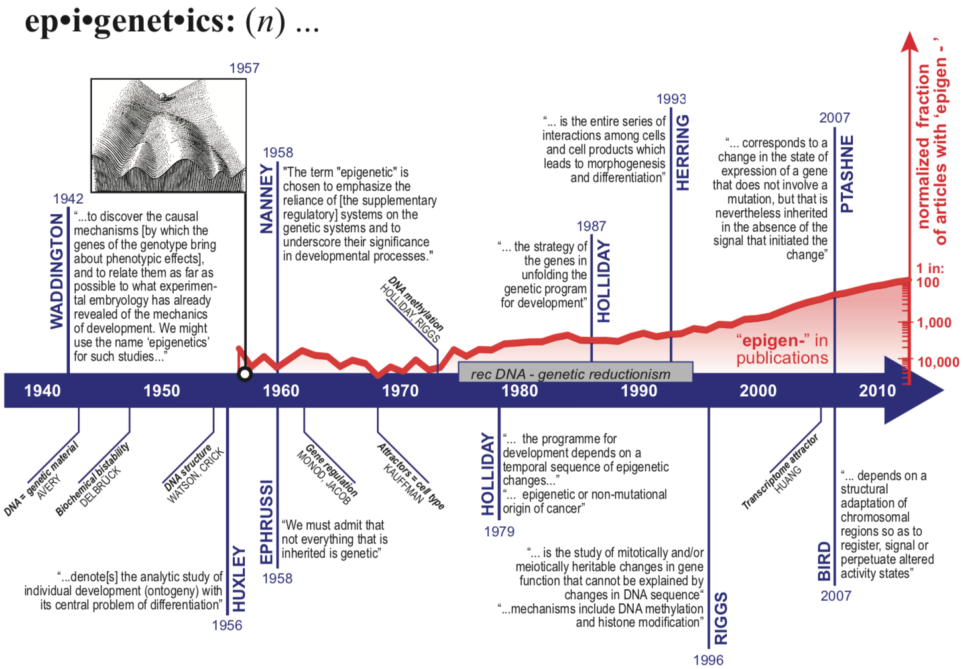
\includegraphics{thesis_files/figure-latex/if1-1} 

}

\caption[History of the term epigenetics]{\textbf{History of the term ‘epigenetics’.} The discovery of
DNA methylation launched the associated modern (molecular) notion of
`epigenetics (1975) and is reflected in the surge of the number of
publications after that. Note the stagnation in the two decades after
that DNA recombinant technology and genetic determinism dominated
mindset in biology (grey horizontal bar). We are now seeing an enormous
increase in the use of the term, as the post-genome era findings
challenge the textbook gene-centred mindset. Textboxes display quotes,
of selected authors (vertical text). The red curve indicates the number
of Medline entries containing the wildcarded search term 'epigen*' per
year, normalized for a number of publications that contain the generic
keywords `cell' and `function'. Diagonal text boxes highlight key
discoveries or findings in biology influencing the history of
epigenetics but not directly related to it. Taken from (\protect\hyperlink{ref-susiarjo2016}{Susiarjo, 2016}).}\label{fig:if1}
\end{figure}
\hypertarget{germline-epigenetics}{%
\section*{Germline epigenetics}\label{germline-epigenetics}}
\addcontentsline{toc}{section}{Germline epigenetics}

\hypertarget{spermatogonial-stem-cells}{%
\subsection*{Spermatogonial Stem Cells}\label{spermatogonial-stem-cells}}
\addcontentsline{toc}{subsection}{Spermatogonial Stem Cells}

The germ stem cells of the seminiferous epithelium in the testis are
known as spermatogonial stem cells (SSCs). They are the building blocks
of spermatogenesis, the mechanism of producing mature male germ cells.
The SSCs are responsible for the continuous creation of the massive
number of sperm cells required for a male's reproductive lifespan. They
are present in the testis from birth and for the rest of the male's
life. SSCs have a dual biological function: they replicate themselves to
maintain the stem cell pool while also generating progenitors that will
differentiate into spermatozoa. They begin life in the testicular
seminiferous tubules and continue to serve this dual purpose throughout
adulthood. SSCs are the male adult stem cells of the seminiferous
epithelium in the testis that are capable of transferring a species'
genome from generation to generation while also possessing the ability
to differentiate into pluripotent stem cells.

In mice, the primordial germ cells (PGCs), the precursors of
prospermatogonia, appear at 5.5 days post-coitum. Prospermatogonia
establishes SSCs shortly after birth (gonocytes). PGCs undergo global
DNA demethylation (which involves the full erasure of parental imprints)
through both active and passive mechanisms as they migrate toward the
gonads. DNA methylation (DNAme) is gradually restored after that
(between embryonic day 13.5 {[}E13.5{]} and E16.5), and both maternal and
paternal-specific imprints are believed to be completely formed by birth
in male prospermatogonia (\protect\hyperlink{ref-hammoud2015}{Hammoud et al., 2015}).

The prospermatogonia are mitotically arrested at birth, but they begin
cycling on postnatal days 1--2 (PND1 -- PND2). A population of
spermatogonial cells continues to proliferate throughout the first week
after birth, giving rise to the undifferentiated A\textsubscript{single}, A\textsubscript{paired}, and A\textsubscript{aligned} spermatogonial pools (\protect\hyperlink{ref-kolasa2012}{Kolasa, Misiakiewicz, Marchlewicz, \& Wiszniewska, 2012}). Cycling
spermatogonia proliferate and populate the seminiferous tubule over the
next week (PND3--PND10); here, a subset gives rise to self-renewing
SSCs, while the rest differentiates without self-renewal, resulting in
the first wave of spermatogenesis or commits apoptosis. As a result,
this stage of germ cell growth is critical for initiating and
maintaining male fertility during adulthood. Following puberty, after
35-37 days, SSCs go through many phases of proliferation, eventually
forming sister stem cells that will maintain a stable pool or more
differentiated intermediates that will initiate meiosis I and II and
form mature sperm cells. Please see Figure \ref{fig:if2} for an overview. These transitions are timed to correlate with
global epigenome shifts, which represent the spermatogonial cell's
developmental path, current transcriptional program, and future
commitment to differentiation. Since the transcriptome and epigenetic
landscape of spermatogonial stem cells is so complex during
proliferation and differentiation, drastic changes in the environment
may not go unnoticed.


\begin{figure}[htbp]

{\centering 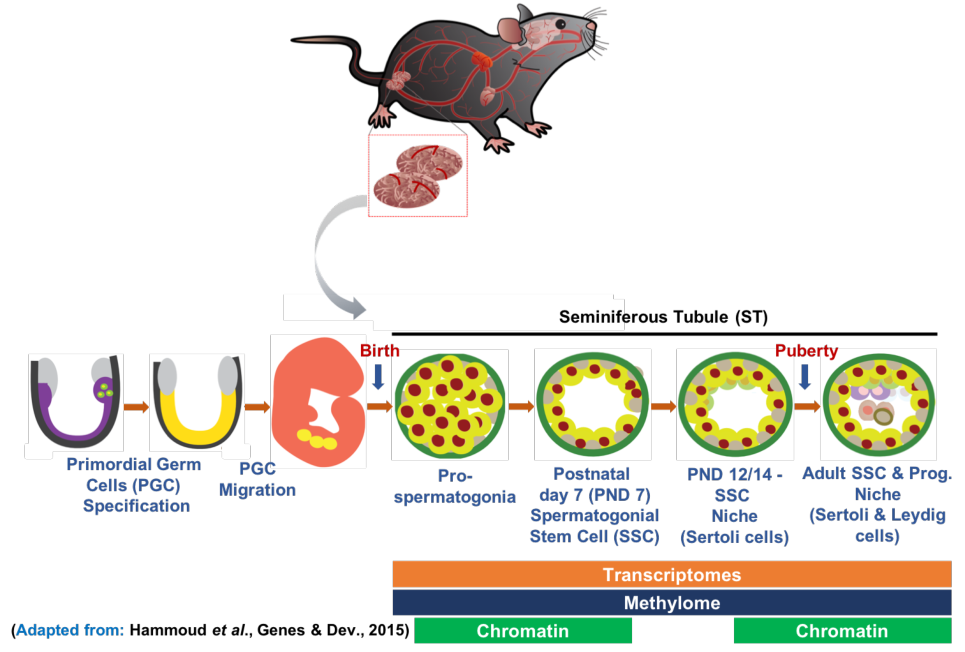
\includegraphics{thesis_files/figure-latex/if2-1} 

}

\caption[Graphical summary of the biology of germline stem cell specification and transitions]{\textbf{Graphical summary of the biology of germline stem cell specification and transitions.} Adapted from (\protect\hyperlink{ref-hammoud2015}{Hammoud et al., 2015})}\label{fig:if2}
\end{figure}
It is difficult to distinguish SSCs from progenitor spermatogonia that
don't have stem cell activity and are committed to
differentiation. Specific cell surface markers like Thy1 and TSPAN8 can
be used to enrich SSCs. Further, cells extracted from Id4-eGFP
transgenic mice that express a high amount of GFP signal, and
combinations of reporter gene and cell surface marker signal can be used
to further enrich the population (\protect\hyperlink{ref-chan2014}{F. Chan et al., 2014}; \protect\hyperlink{ref-mutoji2016}{Mutoji et al., 2016}).

\hypertarget{reprogramming}{%
\subsection*{Reprogramming}\label{reprogramming}}
\addcontentsline{toc}{subsection}{Reprogramming}

Reprogramming refers to the erasure and remodelling of epigenetic
markers such as DNAme throughout mammalian development (\protect\hyperlink{ref-reik2001}{Reik, Dean, \& Walter, 2001}).
Diverse cells and tissues acquire different gene expression patterns
during the evolution of multicellular organisms. Some cells undergo
extensive epigenetic reprogramming in normal developmental or
pathological conditions, which involves the removal of epigenetic marks
in the nucleus and the installation of a new set of marks. Genome-wide
epigenetic reprogramming occurs at stages when the developmental potency
of cells changes. There is passive DNA demethylation and further
reorganization of histone modifications. The epigenetic reprogramming is
likely to be needed for totipotency, correct initiation of embryonic
gene expression, and early lineage development in the embryo. Extensive
epigenetic reprogramming of DNA and histone marks occur in mammalian
development in totipotent early embryos and pluripotent germ cells
(\protect\hyperlink{ref-canovas2016}{Canovas \& Ross, 2016}).

The germ cell lineage is unique in carrying genetic and epigenetic
information from one generation to the next. In the germline, epigenetic
reprogramming resets genomic potential and erases epigenetic memory.
Epigenetic reprogramming involves genome-wide demethylation of 5mC,
which is important for genome imprinting, X inactivation, transposon
silencing, centromeric/telomeric structural stability, and gene
expression (\protect\hyperlink{ref-surani2007}{Surani, Hayashi, \& Hajkova, 2007}). After a sperm fertilizes an ovum, nearly all
epigenetic marks are reprogrammed in two short intervals early in
development. By eliminating random changes in epigenetic marks (i.e.,
epimutations) that have occurred in the germ cells, reprogramming restores the ability
of the fertilized egg cell (i.e., zygote) to develop into all the
different cells types and tissues (\protect\hyperlink{ref-reik2001}{Reik et al., 2001}). During embryo
development, there are two waves of epigenetic reprogramming, Figure \ref{fig:if3}.
After fertilization in the preimplantation embryo (i.e., the
blastocyst), the first phase begins; preimplantation refers to the time
between the embryo implanting and forming a placenta. The embryo in mice
undergoes genome-wide demethylation after fertilization, which is
finished by E5 (\protect\hyperlink{ref-reik2001}{Reik et al., 2001}; \protect\hyperlink{ref-smallwood2012}{Smallwood \& Kelsey, 2012}). The
paternal genome undergoes rapid, active demethylation, whereas the
maternal genome experiences passive demethylation. The embryonic DNA
begins to be re-methylated on day E5 and is finished before birth. The
second wave of epigenetic reprogramming takes place in the germ cells of
the developing embryo, which will eventually give rise to gametes with
sex-specific epigenetic markers (gametogenesis). The methylation
signatures of the parental genomes are found in the PGCs, which are progenitors to both male and female germ cells
in the developing embryo. PGCs are epiblast cells that first appear in
the posterior primitive streak at E7.5, after which they begin to
migrate from E8.5 to the genital ridge, arriving by E11.5. PGCs undergo
rapid demethylation beginning around E7--8, which is completed by
E15--16. In PGCs, parental imprints are erased and totipotency is
restored, followed by the restoration of sex-specific methylation.
Reprogramming is complete in the male germline at birth, but not in the
female germline until adolescence.


\begin{figure}[htbp]

{\centering 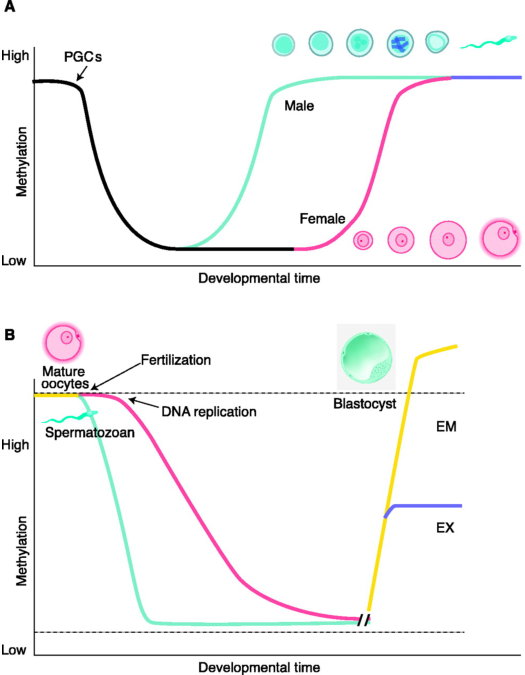
\includegraphics{thesis_files/figure-latex/if3-1} 

}

\caption[Graphical summary of the biology of germline stem cell specification and transitions]{\textbf{Methylation reprogramming in the germline.} \newline \textbf{A:} Primordial germ cells (PGCs) in the mouse become demethylated early in development. Remethylation begins in prospermatogonia on E16 in male germ cells, and after birth in growing oocytes. Some stages of germ cell development are shown. \newline \textbf{B:} Methylation reprogramming in preimplantation embryos. The paternal genome (blue) is demethylated by an active mechanism immediately after fertilization. The maternal genome (red) is demethylated by a passive mechanism that depends on DNA replication. Both are remethylated around the time of implantation to different extents in embryonic (EM) and extraembryonic (EX) lineages. Methylated imprinted genes and some repeat sequences (dashed line) do not become demethylated. Unmethylated imprinted genes (dashed line) do not become methylated. Taken from (\protect\hyperlink{ref-reik2001}{Reik et al., 2001}).}\label{fig:if3}
\end{figure}
Embryonic development involves epigenetic reprogramming to replenish
totipotency from a germline state in each generation. To begin with,
because there is no hereditary germplasm and germ cell precursors are
formed from a post-implantation epiblast that has acquired epigenetic
markers throughout early development, a germline reprogramming phase may
be required to ensure that this acquired information is erased. Then, in
the post-implantation epiblast, the parent-of-origin markers of mature
gametes fuse in the zygote and are passed down to nascent PGCs from
their predecessors. Another goal could be to reverse the effects of
accumulating epigenetic changes that are influenced by both genetic and
environmental factors. However, epigenetic information can be inherited
through the germline (or after fertilization) on occasion, which is most
likely due to insufficient germline erasure. Finally, demethylation in
the germline may have the added benefit of reducing the frequency of
mutations caused by 5-methylcytosine (5mC) deamination.

\hypertarget{epigenetic-inheritance}{%
\section*{Epigenetic Inheritance}\label{epigenetic-inheritance}}
\addcontentsline{toc}{section}{Epigenetic Inheritance}

Inheritance is the process of passing traits or information from one
generation of individuals or cells to the next. Charles Darwin proposed
natural selection as the primary mechanism for species evolution in his
1859 book: ``On the origin of species''. According to Darwin, natural
selection is a key mechanism of evolution, characterized by changes in
the heritable traits of a population over generations. Jean-Baptiste
Lamark was an early proponent of the idea that biological evolution
occurred and proceeded in accordance with natural laws. He is well known
for the principle of ``inheritance of acquired characteristics'', an idea
known as Lamarckism. According to Lamarckian theories of inheritance,
physical traits inherited by a generation during its lifetime (e.g.
strength and body size) are passed down to offspring. In 1868, Darwin
proposed pangenesis theory as a supplement to his 1859 theory of
evolution by natural selection in his book ``The Variation of Animals and
Plants Under Domestication.'' The term pangenesis was coined by Darwin,
with ``pan-'' referring to the whole and ``genesis'' referring to the
origin. Using the term pangenesis, Darwin proposed that all parts of the
parents could contribute to the evolution and development of the
offspring. Darwin's theory of pangenesis was based on the idea that
somatic cells would release `gemmules' or `pangenes' in response to
environmental stimulation (use and disuse), which travelled around the
body but not necessarily in the bloodstream. These pangenes were
microscopic particles that supposedly contained information about the
characteristics of their parent cell, and Darwin believed that they
eventually accumulated in germ cells, where they could pass on the newly
acquired characteristics of the parents to the next generation
(\protect\hyperlink{ref-darwin1871}{Darwin, 1871}). As a result, Darwin advocated Lamarckian use and disuse
inheritance, as well as Lamarckian soft inheritance. In the 1880s,
August Weismann challenged this concept. Weismann proposed the germ
plasm theory, which states that germ cells in the gonads contain
information that is passed down from generation to generation unaffected
by experience and independent of somatic cells (\protect\hyperlink{ref-weismann1893}{Weismann, 1893}).
Hereditary information is only transferred from germline cells to
somatic cells. This is referred to as the Weismann barrier.

However, recent epigenetic discoveries have revealed that acquired
traits can be passed down to future generations. Our recent work showed
that serum from adult male mice exposed to postnatal stress, injected
chronically to naïve males, can induce metabolic symptoms associated with
stress in the offspring of the injected males (\protect\hyperlink{ref-vansteenwyk2020}{van Steenwyk et al., 2020}). Also,
we identified circulating extracellular vesicles as vectors of
communication with germ cells that can reproduce symptoms of exposure in
the offspring when injected into fathers in vivo (\protect\hyperlink{ref-alshanbayeva2021}{Alshanbayeva, Tanwar, Roszkowski, Manuella, \& Mansuy, 2021}).
These results highlight the importance of circulating factors in the
mechanisms of epigenetic inheritance, \protect\hyperlink{chapter2}{Chapter 2}.

\hypertarget{tei}{%
\subsection*{Transgenerational Epigenetic Inheritance}\label{tei}}
\addcontentsline{toc}{subsection}{Transgenerational Epigenetic Inheritance}

The transmission of epigenetic information from one generation to the
next is referred to as intergenerational epigenetic inheritance, while
that across multiple generations is referred to as transgenerational
epigenetic inheritance. Both intergenerational and transgenerational
imply the parents' exposure to the environmental factor in question, as
well as the gametes they already have. Transgenerational exposure refers
to people who have never been specifically exposed to the environmental
factor during their lifetime (either as individuals or as future
gametes). This may be the third generation after in utero exposure or
the second generation after preconception exposure. It is assumed that
fetal or in utero exposure to an environmental factor is not heritable
because the offspring are specifically exposed. However, the mechanisms
of adverse development following in utero exposure to drugs, alcohol,
diet, and other factors also influence offspring through epigenetic
mechanisms.

\hypertarget{reprogramming-in-epigenetic-inheritance}{%
\subsection*{Reprogramming in epigenetic inheritance}\label{reprogramming-in-epigenetic-inheritance}}
\addcontentsline{toc}{subsection}{Reprogramming in epigenetic inheritance}

Epigenetic reprogramming refers to the process of removing and resetting
relevant epigenetic information in germ cells, which is primarily
accomplished through DNA demethylation. Epigenetic reprogramming
prevents the transmission of epigenetic information from mature gametes,
which is in line with the germ-plasm theory of Weissman (\protect\hyperlink{ref-weismann1893}{Weismann, 1893}).
The extent of epigenetic reprogramming, however, is unknown, leaving the
question of how much epigenetic information from adult gametes is
preserved in the embryo unanswered. In mammals, DNAme and histone marks
are effectively reset during reprogramming both in the germline, and in
the zygote immediately after conception, leaving epigenetic changes with
minimal possibility of passing down. Evidence for the survival of
histone modifications across reprogramming has been identified in sperm,
where histones are largely replaced by protamines. Surprisingly,
H3K27me3 enrichment has been discovered in reprogramming resistant sperm
nucleosomes (\protect\hyperlink{ref-casas2020}{Casas \& Vavouri, 2020}), suggesting that this mark may be a hereditary
signal. Further, findings in (\protect\hyperlink{ref-kremsky2020}{Kremsky \& Corces, 2020}) imply that transcription
factors can operate as epigenetic information carriers during germ cell
and pre-implantation development by maintaining the CpG methylation
state.

\hypertarget{models-of-epigenetic-inheritance}{%
\section*{Models of Epigenetic Inheritance}\label{models-of-epigenetic-inheritance}}
\addcontentsline{toc}{section}{Models of Epigenetic Inheritance}

Given limitations such as the inability to conduct controlled
experiments in humans and the availability of data for successive
generations, rodent models have become critical for correlating human
findings (\protect\hyperlink{ref-jawaid2021}{Jawaid, Jehle, \& Mansuy, 2021}) and to investigate the penetrance of effects
across generations to provide mechanistic insight. There are several
experimental paradigms for studying epigenetic inheritance. In mammals,
dietary changes, stress, medications, and environmental toxins have all
been linked to altered phenotypes in offspring (\protect\hyperlink{ref-gapp2018}{K. Gapp \& Bohacek, 2018}). Epigenetic
inheritance appears to be initiated or modulated by mutations in the
epigenetic machinery, such as DNA/RNA methylation enzymes or histone
modification complexes, such as overexpression of \emph{Kdm1a}, an H3K4me3
demethylase in mice (\protect\hyperlink{ref-siklenka2015}{Siklenka et al., 2015}).

Alternatively, environmental perturbations may initiate epigenetic
inheritance, with various insults leading to offspring phenotypes in a
variety of model systems (\protect\hyperlink{ref-jawaid2019}{Jawaid \& Mansuy, 2019}). Environmental factors like
vinclozolin (an antiandrogenic compound), methoxychlor (an estrogenic
compound), stress responses, high-fat diet, high-sugar diet, low-protein
diet, air pollutant exposure in pregnant mice, in utero Bisphenol-A (BPA),
di(2- Ethylhexyl) phthalate (DEHP) and dibutyl phthalate (DBP) exposure
in rats, in utero exposure to jet fuel (JP-8) in mice, in utero valproic
acid exposure in mice, olfactory fear conditioning in Filial 0 (F0) mice, and
Female mice fed a high-fat/ high-sugar diet have been linked to
epigenetic inheritance (\protect\hyperlink{ref-bohacek2015}{Bohacek \& Mansuy, 2015}; \protect\hyperlink{ref-hanson2016}{Hanson \& Skinner, 2016}; \protect\hyperlink{ref-heard2014}{Heard \& Martienssen, 2014}; \protect\hyperlink{ref-mao2017}{Mao, Li, Liu, \& Chi, 2017}; \protect\hyperlink{ref-nagy2015}{Nagy \& Turecki, 2015}; \protect\hyperlink{ref-rando2016}{Rando, 2016}; \protect\hyperlink{ref-schaefer2015}{Schaefer \& Nadeau, 2015}). These models shed new light on
the mechanisms of epigenetic inheritance. However, distinguishing
evidence of epigenetic mark transmission from the evidence of exposure
transmission is difficult.

\hypertarget{msus-mouse-model}{%
\subsection*{MSUS mouse model}\label{msus-mouse-model}}
\addcontentsline{toc}{subsection}{MSUS mouse model}

\textbf{A unique transgenerational model to assess the effects of trauma:}
unpredictable maternal separation combined with unpredictable maternal
stress (MSUS) is a firmly established transgenerational model in the
Mansuy lab, that does not involve any chemical or mutagenic agent but,
depends only on psychological and emotional trauma, Figure \ref{fig:if4}. It is an
ideal model to study the possible transgenerational effects of life
experiences on the genome and the epigenome.


\begin{figure}[htbp]

{\centering 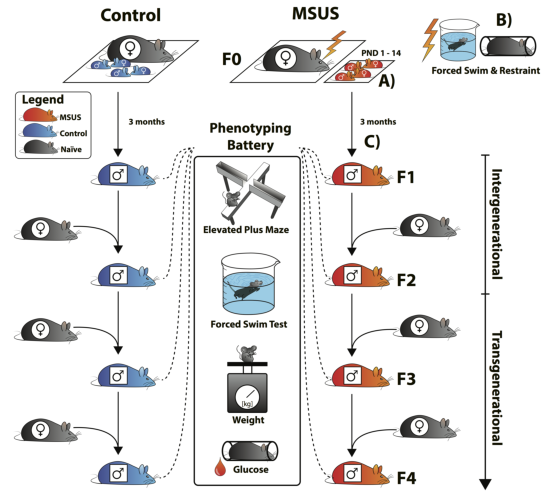
\includegraphics{thesis_files/figure-latex/if4-1} 

}

\caption[MSUS paradigm]{\textbf{MSUS paradigm.} MSUS consists of \textbf{(A)} separating mouse pups (F1) from their mother (F0, naïve primiparous control females mated with naïve males) daily for 3 hours per day at an unpredictable time during the 12 hours active cycle, starting 1 day after birth (postnatal day 1, PND1) until PND14. \textbf{(B)} During separation, dams are exposed to an additional unpredictable stressor by being subjected to either, a forced swim in 18°C water for 5 minutes or a 20-minute physical restraint in a tube, anytime (unpredictably) during the 3 hours. From PND15, mice are left undisturbed with their mother until PND21 (no further MSUS), are then weaned at PND21 and raised normally until adulthood \textbf{(C)}. Control litters are raised normally (left). Males used to generate the pups are removed from the breeding cage shortly after mating thus, fathers never encounter their offspring and do not contribute to their rearing. When adult (3--8 months of age), F1 males are paired with naïve primiparous control females to sire the F2 generation, then F2 and F3 males are bred with naïve primiparous control females to generate an F3 and F4 offspring, respectively. Males from each generation are tested on the elevated plus-maze, forced swim test, weight measurements and glucose response after physical restraint. MSUS is applied only to F1 mice, mice from F2, F3 and F4 generations are not exposed to any manipulation. Phenotypes transmitted from father to offspring are intergenerational, phenotypes that persist from father to offspring then grand-offspring or great grand-offspring are transgenerational. Taken from (\protect\hyperlink{ref-vansteenwyk2018}{van Steenwyk, Roszkowski, Manuella, Franklin, \& Mansuy, 2018}).}\label{fig:if4}
\end{figure}
MSUS consists in separating
mouse pups from their mother unpredictably (any time during the day)
each day for 3 hours from postnatal day 1 (PND1) to PND14 and exposing the mothers to stressful situations such as restraint stress or
forced swim in cold water (18ºC), unpredictably during separation. F1 generation males are mated with naïve control females, and F2
males are mated with control females to obtain F3. MSUS induces several
behavioural symptoms including depression, increased risk-taking,
antisocial behaviours and memory deficits, and metabolic alterations
across several generations (\protect\hyperlink{ref-franklin2010}{Franklin et al., 2010a}; \protect\hyperlink{ref-vansteenwyk2018}{van Steenwyk et al., 2018}). Further,
metabolic phenotypes like decreased bodyweight, insulin hypersensitivity
and glucose intolerance are also observed. For studying the molecular
mechanisms of epigenetic inheritance, a number of high-throughput sequencing (HTS) datasets have been
collected and sequenced, Figure \ref{fig:if5}.


\begin{figure}[htbp]

{\centering 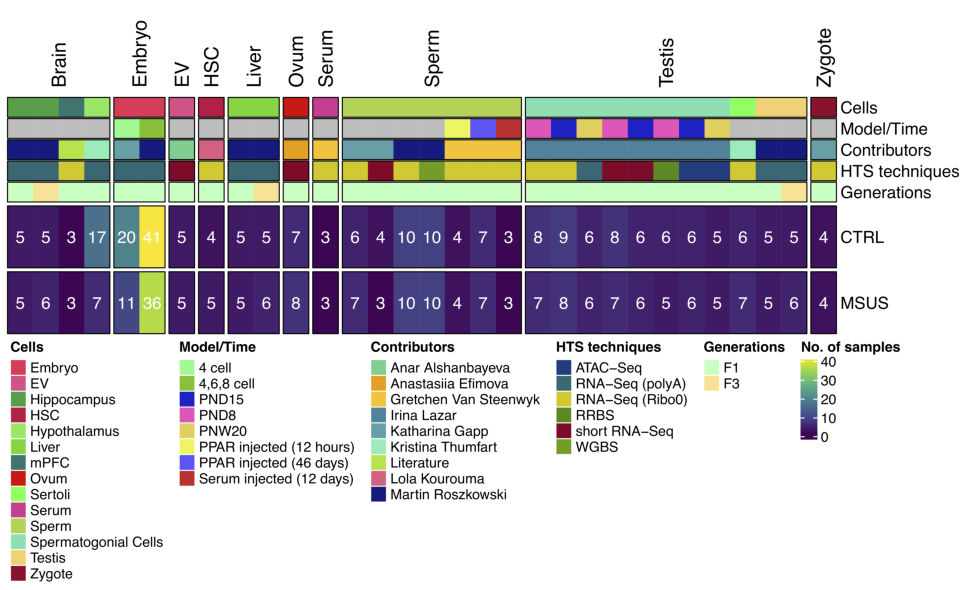
\includegraphics{thesis_files/figure-latex/if5-1} 

}

\caption[Dataset collected from the MSUS model]{\textbf{Dataset collected from the MSUS model.}}\label{fig:if5}
\end{figure}
\hypertarget{vectors-of-epigenetic-inheritance}{%
\section*{Vectors of epigenetic inheritance}\label{vectors-of-epigenetic-inheritance}}
\addcontentsline{toc}{section}{Vectors of epigenetic inheritance}

Epigenetic marks, such as DNAme, histone modifications, and non-coding
RNAs, have been proposed as information-carrying vectors passed down
through generations. These three candidates have been investigated in a
variety of epigenetic inheritance paradigms. It is hypothesized that stable changes in
epigenetic marks caused by an environmental insult (epimutations) may
affect gene expression or chromatin stability, increasing the risk of a
phenotype or disease in offspring (Miska and Ferguson-Smith, 2016).
DNAme, histone modifications, RNA, and ncRNAs are all interconnected and
interdependent within individual cells. They are likely to act in a
coordinated and collaborative manner to cause disease phenotypes in the
context of epigenetic inheritance.

\hypertarget{dna-methylation}{%
\subsection*{DNA methylation}\label{dna-methylation}}
\addcontentsline{toc}{subsection}{DNA methylation}

The most common type of DNAme in mammals is cytosine residue
methylation. Cytosine residues are methylated on the 5' carbon and are
referred to as 5-methylcytosines (5mC). Methylation of a cytosine
residue is a binary process -- either methylation or non-methylation. In
mammals, DNA methylation is typically found in the context of CpG
dinucleotides (\protect\hyperlink{ref-bird2002}{Bird, 2002}). Cytosine methylation can be copied from one
DNA strand to the next in this manner during replication and meiosis.
DNAme patterns, on the other hand, are dynamic. The patterns of DNAme
vary over time and space, changing during development and differing
between cell types (\protect\hyperlink{ref-luo2018}{Luo, Hajkova, \& Ecker, 2018}). DNA methyltransferase (DNMT) enzymes
methylate cytosine residues. DNMT1 is a methyltransferase that reads
hemimethylated DNA after cell division and adds methylation to the newly
synthesized strand (\protect\hyperlink{ref-chen2011}{Z. Chen \& Riggs, 2011}). The de novo methyltransferases DNMT3a
and 3b can add methylation to previously unmethylated residues
(\protect\hyperlink{ref-smith2013}{Smith \& Meissner, 2013}). Although DNAme in gene control regions is generally
associated with gene repression, its precise role in gene regulation is
likely locus dependent (\protect\hyperlink{ref-deaton2011}{Deaton \& Bird, 2011}). Methylated DNA is a true
epigenetic mark because there are ``readers'' that preferentially
recognize 5mC and can interpret the methylation mark's meaning
(\protect\hyperlink{ref-zhu2016a}{H. Zhu, Wang, \& Qian, 2016}). Many properties of DNAme make it an appealing mechanistic
candidate for epigenetic inheritance, including the following: it can be
environmentally modulated; machinery exists to replicate methylation
patterns onto newly synthesised DNA, making it mitotically heritable;
and methylated loci resistant to epigenetic reprogramming have been
identified in the zygote and germline. Disruption of the DNAme machinery
may also play a role in the initiation of EI.

\hypertarget{histone-modifications}{%
\subsection*{Histone modifications}\label{histone-modifications}}
\addcontentsline{toc}{subsection}{Histone modifications}

In somatic cells, DNA is wrapped around an octameric core of histone
proteins (H2A, H2B, H3, and H4) to form a nucleosome (\protect\hyperlink{ref-marmorstein2009}{Marmorstein \& Trievel, 2009}).
Histones' N-terminal tails and globular domains undergo
post-translational modifications (PTMs). Histone modifications are
dynamic during development, vary across tissues, are regulated by
specific enzymes, play a significant role in gene expression, and
interact with other epigenetic control systems such as DNAme
(\protect\hyperlink{ref-barth2010}{Barth \& Imhof, 2010}). On the histone tails, there are over 60 different amino
acid residues where modifications have been detected (\protect\hyperlink{ref-iwasaki2013}{Iwasaki et al., 2013}).
Histones can undergo various modifications, including acetylation,
methylation, phosphorylation, ubiquitination and sumoylation among
others (\protect\hyperlink{ref-kouzarides2007}{Kouzarides, 2007}). Histone methyltransferase (HMT) enzymes
methylate histones on Lysine (K) and Arginine (R) amino acids. Histone
lysine residues can be mono-, di-, or tri-methylated, and these
modifications can function as either active or repressive marks.
Methylation of H3K4, H3K36, and H3K79 is associated with transcriptional
activation, whereas methylation of H3K9, H3K27, and H4K20 is associated
with transcriptional repression (\protect\hyperlink{ref-sims2006}{Sims, Houston, Magazinnik, \& Rice, 2006}; \protect\hyperlink{ref-vakoc2006}{Vakoc, Sachdeva, Wang, \& Blobel, 2006}). These
modifications can influence chromatin packaging and nucleosome
positioning. Histone modifications, like DNAme, are spatially and
temporally dynamic. Certain histone modifications, such as
trimethylation of lysine 27 on histone 3 (H3K27me3), are generally
associated with gene repression, whereas acetylation of the same residue
(H3K27ac) is generally associated with gene activation (\protect\hyperlink{ref-lawrence2016}{Lawrence, Daujat, \& Schneider, 2016}).
Histone modifications regulate gene expression by recruiting protein
complexes and controlling the accessibility of DNA to the transcription
machinery (\protect\hyperlink{ref-lawrence2016}{Lawrence et al., 2016}). Histone modifications are a plausible
mechanistic candidate in epigenetic inheritance because they can be modulated by the
environment. During epigenetic reprogramming, some histone modifications
in the germline and zygote are retained. Histones are spread onto newly
assembled chromatin by sophisticated machinery (\protect\hyperlink{ref-marmorstein2009}{Marmorstein \& Trievel, 2009}).
However, it is still unclear how histone codes are maintained during
mitosis and meiosis (\protect\hyperlink{ref-erkek2013}{Erkek et al., 2013}). Furthermore, during spermatogenesis,
most histones are removed and replaced with protamines (\protect\hyperlink{ref-casas2014}{Casas \& Vavouri, 2014}).
Sperm contains protamine modifications that are similar to histone
modifications (\protect\hyperlink{ref-brunner2014}{Brunner, Nanni, \& Mansuy, 2014}), despite this, their functional
significance remains unknown, particularly during epigenetic
inheritance. Disruption of the machinery that regulates histone
modification could also be a key initiator of epigenetic inheritance (\protect\hyperlink{ref-siklenka2015}{Siklenka et al., 2015}). H3K9
and H3K27 methylation appear to be the most likely to be epigenetic
among the various histone lysine methylation states, not only because
they are key regulators of classic epigenetic phenomena (\protect\hyperlink{ref-huang2013}{C. Huang, Xu, \& Zhu, 2013}).
According to one model of epigenetic inheritance, marked parental
histones inherited via DNA replication recruit histone modifiers to
deposit similar marks on new adjacent nucleosomes, reestablishing the
previous local landscape of histone modification (\protect\hyperlink{ref-saxton2019}{Saxton \& Rine, 2019}). These
findings suggest that histone modifications can aid in epigenetic
inheritance, though such a mechanism is normally obscured by H3K9
demethylation activity (\protect\hyperlink{ref-saxton2019}{Saxton \& Rine, 2019}).

\hypertarget{rna}{%
\subsection*{RNA}\label{rna}}
\addcontentsline{toc}{subsection}{RNA}

One haploid copy of the genome exists in the sperm nucleus, which is
transcriptionally silent and not replicated due to the packaging of
sperm chromatins during spermiogenesis. Also, the sources of sperm RNAs
are unknown. Some RNAs are probably expressed endogenously within germ
cells, but considering that short RNAs have been demonstrated to impact
gene expression outside of their tissue of origin, sperm RNA could come
from elsewhere. Because RNAs are easily degraded, they are most likely
transported with protein chaperones and, more likely, enclosed in
extracellular vesicles. For example, in epididymosomes, which are
extracellular vesicles that are released from the epididymal epithelium
contain proteins, ncRNAs and a distinct set of lipids that are
transferred to spermatozoa while they pass through the different
epididymal regions (\protect\hyperlink{ref-sullivan2016}{Sullivan, 2016}). Aside from epididymosomes, RNAs have
been found in exosomes and high-density lipoproteins (HDLs) in the
bloodstream, as well as vesicles secreted by prostate cells
(protostomes) and Sertoli cells, which come into direct contact with
developing sperm. These interactions have not been studied in the
context of transgenerational inheritance. Microinjections of RNA
mixtures were used to recapitulate mutant phenotypes in functional tests
of RNAs contribution to inheritance patterns. These findings imply that
RNA plays a significant role in non-genetic inheritance. It is unclear
how these transient RNA molecules can mediate epigenetic inheritance
across cell divisions and generations on their own. Nonetheless, a
growing body of evidence suggests that RNA may aid in the stable
propagation of paternal effects from the soma to the germline, where
they will be inherited by the next generation (\protect\hyperlink{ref-andersson2014}{Andersson et al., 2014}; \protect\hyperlink{ref-gapp2020}{K. Gapp, van Steenwyk, et al., 2020}; \protect\hyperlink{ref-vansteenwyk2020}{van Steenwyk et al., 2020}).

\hypertarget{non-coding-rna}{%
\subsection*{Non-coding RNA}\label{non-coding-rna}}
\addcontentsline{toc}{subsection}{Non-coding RNA}

ncRNAs are broadly classified into two types: 1) long-ncRNA, greater
than 200 nucleotides in length (lncRNAs) (\protect\hyperlink{ref-li2012}{Z. Li et al., 2012}) and 2) small-ncRNA,
less than 200 nucleotides (sncRNA) (\protect\hyperlink{ref-bouckenheimer2018}{Bouckenheimer et al., 2018}). Small
regulatory RNAs (siRNAs, miRNAs, tRNAs, and piRNAs) are non-coding RNAs
that are expressed in the majority of eukaryotic cells. These small RNAs
are bound by the Argonaute (AGO) or PIWI proteins and function as
specificity factors (guide RNAs) to regulate other homologous RNAs at
the transcription, stability, and translation levels. Small RNAs are
found in the nuclei of most eukaryotes, where they regulate genome
stability, heterochromatin formation, and transcription. ncRNAs are
uniquely suited to transmit information across generations. A variety of
ncRNA species can be found in both sperm and oocytes (\protect\hyperlink{ref-rando2016}{Rando, 2016}; \protect\hyperlink{ref-veselovska2015}{Veselovska et al., 2015}). There is evidence that sperm can acquire ncRNAs from
surrounding somatic tissues (\protect\hyperlink{ref-robles2019}{Robles, Valcarce, \& Riesco, 2019}). Thus, RNAs can circumvent and
penetrate the theoretically impenetrable wall between somatic cells and
the germline (the so-called Weismann barrier). This has significant
implications for our understanding of epigenetic inheritance as a result
of adult-life environmental insults. However, it is currently unknown
how epigenetic messages transmitted by RNA are maintained across
multiple cell divisions, let alone multiple generations.

\hypertarget{transcription-factors}{%
\subsection*{Transcription factors}\label{transcription-factors}}
\addcontentsline{toc}{subsection}{Transcription factors}

Transcription factors (TFs) may also act as epigenetic information
carriers. TFs are proteins that play a role in the
process of transcribing DNA to RNA. TFs are found on the genomes of
mature gametes, and there is evidence that TF binding can influence
DNAme at the binding sites (\protect\hyperlink{ref-jones2001}{Jones \& Takai, 2001}; \protect\hyperlink{ref-smith2013}{Smith \& Meissner, 2013}). CpG sites bound by
TFs during germ cell re-methylation are protected from methylation
throughout development (\protect\hyperlink{ref-kremsky2020}{Kremsky \& Corces, 2020}). During PGC and preimplantation
development, DNAme can only occur at CpGs that are resistant to
demethylation. This is due to the fact that TF binding during the
re-methylation phase maintains the methylation status between
generations (\protect\hyperlink{ref-kremsky2020}{Kremsky \& Corces, 2020}). This suggests that transcription factors can
act as carriers of epigenetic information during germ cell and
pre-implantation development by maintaining CpG methylation status, and
serve as the foundation for a mechanistic description of the
transgenerational transmission of such information in mammals
(\protect\hyperlink{ref-kremsky2020}{Kremsky \& Corces, 2020}). Mammalian gametes contain complex patterns of 3D
interactions that can also be transmitted to the zygote after
fertilization (\protect\hyperlink{ref-jung2019}{Jung et al., 2019}). TFs may remain bound to chromatin after
fertilization and influence gene expression in the developing embryo.
According to a recent publication, BPA, either directly or indirectly,
induces the binding of TFs at different regions of the genome in F1
generation sperm, altering the 3D organization of chromatin in mature F1
generation sperm, many of which are conserved in subsequent generations
(\protect\hyperlink{ref-jung2020}{Jung et al., 2020}). Thus, TFs are a plausible candidate for transmitting
epigenetic information.

\hypertarget{extracellular-vesicles}{%
\subsection*{Extracellular vesicles}\label{extracellular-vesicles}}
\addcontentsline{toc}{subsection}{Extracellular vesicles}

All cells can secrete various types of membrane vesicles known as
extracellular vesicles (EVs). EVs vary greatly in size (30 nm to several
micrometres in diameter), chemical composition, secretion mechanism and
carrying molecules, all of the properties that lead to their different
functions. EVs mediate cell-to-cell communication by activating
receptors on the surface of acceptor cells (\protect\hyperlink{ref-bonsergent2021}{Bonsergent et al., 2021}) and play
roles in a variety of physiological and pathological processes,
including blood coagulation, inflammation, stem cell expansion, neuronal
communication, and tumorigenesis (\protect\hyperlink{ref-locicero2015}{Lo Cicero, Stahl, \& Raposo, 2015}). There are two major EV
biogenesis pathways. The first biogenesis pathway buds EVs directly from
the plasma membrane, resulting in what is known as microvesicles. The
second biogenesis pathway involves intraluminal vesicle release caused
by multivesicular endosome fusion with the plasma membrane, resulting in
the formation of exosomes. Exosomes and microvesicles contain cargoes
such as nucleic acids, proteins and lipids, RNAs (extracellular RNAs,
exRNAs) and DNA (\protect\hyperlink{ref-obrien2020}{O'Brien, Breyne, Ughetto, Laurent, \& Breakefield, 2020}). The majority of known ncRNA biotypes,
including small nuclear RNAs, small nucleolar RNAs (snoRNAs), rRNAs,
lncRNAs, piRNAs, tRNAs,
mitochondrial RNAs, Y RNAs, and vault RNAs (vtRNAs), have been
discovered in EVs in more comprehensive studies (\protect\hyperlink{ref-abels2016}{Abels \& Breakefield, 2016}; \protect\hyperlink{ref-obrien2020}{O'Brien et al., 2020}). ExRNA extraction, purification, and sequencing methods are
much more susceptible to contamination and artefacts than cellular RNA
preparations, due to the low amount of RNA available from EVs. As a
result, analyzing exRNA samples can be difficult, and a specific tool
for EV ncRNA data analysis has been developed (\protect\hyperlink{ref-rozowsky2019}{Rozowsky et al., 2019a}). A number
of studies have shown the role of extracellular vesicles in epigenetic
inheritance. Also, we found that extracellular vesicles are vectors of
communication with the germline that play a role in epigenetic
inheritance (\protect\hyperlink{ref-alshanbayeva2021}{Alshanbayeva et al., 2021}), \protect\hyperlink{chapter2}{Chapter 2}.

\hypertarget{challenges-in-data-analysis}{%
\section*{Challenges in data analysis}\label{challenges-in-data-analysis}}
\addcontentsline{toc}{section}{Challenges in data analysis}

\hypertarget{multi-omics-data-integration}{%
\subsection*{Multi-omics data integration}\label{multi-omics-data-integration}}
\addcontentsline{toc}{subsection}{Multi-omics data integration}

A single omics analysis may not provide enough information to provide a
deep understanding of a biological system, but combining multiple omics
experiments and data analyses can provide a more holistic view of a
system. Performing different experiments on the same or different
samples from the same biological conditions, such as RNA sequencing (RNA-seq), Assay for Transposase-Accessible Chromatin sequencing (ATAC-seq),
chromatin immunoprecipitation with sequencing (ChIP-seq), and Bisulfite sequencing (BS-seq), results in multi-dimensional omics datasets, which
enable the study of relationships between different biological
processes, such as gene expression, chromatin accessibility, histone
modifications, transcription factor binding, and DNAme, as well as the
leveraging of multiple data types to draw inferences about these
processes. Data integration is the process of combining disparate
sources of information in order to gain a better understanding of
complex systems. The researchers execute two forms of data integration:
custom or ad-hoc integration and more systematic integration.

\hypertarget{ad-hoc-approaches}{%
\subsubsection*{Ad-hoc approaches}\label{ad-hoc-approaches}}
\addcontentsline{toc}{subsubsection}{Ad-hoc approaches}

Integrating BS-seq data with RNA-seq is one example of an ad-hoc
technique. The expressed genes are known to be demethylated. As a
result, the methylation values of the promoters can be linked to the
genes that are expressed. Integrating ATAC-seq data with RNA-seq data
can be used to analyze TF activity. Regions with
increased accessibility and expression would show a TF's role as an
activator, while regions with increased accessibility and decreased
expression would represent a TF's role as a repressor. For this, a tool
exists, diffTF (\protect\hyperlink{ref-berest2019}{Berest et al., 2019}), which estimates differential TF activity
based on expression and chromatin data. The ad-hoc methods are
scientifically motivated and produce biologically relevant outcomes.
However, these ad-hoc approaches have several drawbacks, such as the
need for extensive exploratory investigation and the inability to be
applied consistently to all projects. Furthermore, these methods are
frequently applied to a maximum of two omics datasets.

\hypertarget{systematic-approaches}{%
\subsubsection*{Systematic approaches}\label{systematic-approaches}}
\addcontentsline{toc}{subsubsection}{Systematic approaches}

Systematic methods developed for data integration in biological research
can be classified into three types: supervised, unsupervised, and
semi-supervised. Unsupervised data integration refers to methods that
draw conclusions from input datasets without the use of labelled
response variables (e.g., factorization, Bayesian, clustering,
dimensionality reduction, coexpression and correlation). On the other
hand, supervised data integration methods take into account phenotype
labels (e.g., control or treatment) and use, for example, machine
learning approaches to evaluate models (network-based and multi-kernel);
semi-supervised data integration methods fall somewhere between
supervised and unsupervised methods and use both labelled and unlabeled
samples to develop a learning algorithm to infer information from
unlabeled samples (\protect\hyperlink{ref-huang2017}{S. Huang, Chaudhary, \& Garmire, 2017}). A few methods for integrating data from
multivariate multi-omics experiments have been developed: Data
Integration Analysis Using Latent Components for Biomarker Discovery
(DIABLO) (\protect\hyperlink{ref-rohart2017}{Rohart, Gautier, Singh, \& Lê Cao, 2017}) - an extension to sparse generalized canonical
correlation analysis (sGCCA) (\protect\hyperlink{ref-tenenhaus2014}{Tenenhaus et al., 2014}), a supervised approach
which seeks for common information across different data types through
the selection of a subset of molecular features; Multi-Omics Factor
Analysis (MOFA) - an unsupervised method for decomposing the sources of
heterogeneity in multi-omics data sets (\protect\hyperlink{ref-argelaguet2018}{Argelaguet et al., 2018}, \protect\hyperlink{ref-argelaguet2020}{2020}) and; mixOmics (\protect\hyperlink{ref-rohart2017}{Rohart et al., 2017}) - a package that hosts
several supervised methods under its umbrella (DIABLO; sparse Partial
Least Square---Discriminant Analysis, PLS-DA (\protect\hyperlink{ref-luxeacao2011}{Lê Cao, Boitard, \& Besse, 2011}) and
Multivariate INTegrative method, MINT (\protect\hyperlink{ref-rohart2017}{Rohart et al., 2017})).

Despite the fact that these tools have addressed critical challenges for
multi-omics applications, they are not without limitations. One of the
major limitations of most of these tools is that they can only
incorporate data from the same omics experiments. This restricts users
to utilize the same samples for all experiments, which is never the case
in biological research due to the limited quantity of components of
interest (DNA or RNA) and the high demand for these components for
library preparation and sequencing. Another issue is that these methods
assume that users have already normalized the data and corrected it for
batches or confounding factors such as cage effect, sample composition,
and time of day (\protect\hyperlink{ref-bruning2016}{Bruning et al., 2016}). Based on the data types, methods should
be able to optimally normalize the data and correct it for confounding
factors using supervised learning, which could improve uniformity,
robustness, and precision. Another disadvantage is that some of the
existing methods necessitate exploratory analysis prior to data
integration. Exploratory data analysis is a critical process in many
data science projects that requires advanced coding skills and takes a
significant amount of time. The method should be able to perform
automated data cleaning functions, such as outlier clipping, missing
value imputation, and zero-variance variables, depending on the data
types. It should also aid in exploratory analysis by providing summary
statistics and plots for visual examination. Finally, most existing
methods are designed to work with linear relationships and thus cannot
be applied to more complex datasets that are related in a non-linear
manner.

To summarize, integrating diverse and huge omics data is both a
conceptual and practical problem in data analysis. Data integration has
been used in omics research since the beginning of the era, and it is
both a challenge and an opportunity. It is surely growing more popular.
We devised and implemented a more straightforward and scientifically
motivated approach to integrate multi-omics datasets, involving more
than two omics datasets, please see \protect\hyperlink{methods}{Methods} and \protect\hyperlink{chapter1}{Chapter 1}.

\hypertarget{short-rna-data-analysis}{%
\subsection*{Short RNA data analysis}\label{short-rna-data-analysis}}
\addcontentsline{toc}{subsection}{Short RNA data analysis}

Short RNAs are a type of non-coding RNA that plays an important role in
nearly all aspects of organismal development in both health and disease.
Despite their importance in a wide range of biological processes,
analyzing short RNA sequencing data remains a difficult task.
Specifically, a number of computational challenges arise when analyzing
short RNA sequencing:
\begin{itemize}
\item
  Even after size selection, we expect to sequence other RNA biotypes
  in addition to short RNAs.
\item
  Short RNAs have a length of less than 200bp, often much shorter
  (e.g.~miRNAs at 21-22bp), and can therefore often map to multiple
  positions. In this case, standard pipelines either map the reads
  randomly to one position, making it difficult to determine their
  true origin, or they are discarded, resulting in a large proportion
  of reads being lost.
\item
  Many short RNAs are post-transcriptionally modified. For example,
  tRNAs receive a ``CCA'' sequence at the 3' end (\protect\hyperlink{ref-hou2010}{Hou, 2010}),
  additionally, Histidine tRNAs receive a ``G'' sequence at the 5' end
  (\protect\hyperlink{ref-cooley1982}{Cooley, Appel, \& Soll, 1982}), resulting in an unalignment problem.
\item
  Because of their biogenesis, short RNAs often overlap multiple
  features. For example, mature miRNAs overlap with precursors, which
  can result in misassignment.
\item
  rRNAs are typically masked in the genome, and the Ensembl
  (\protect\hyperlink{ref-howe2021}{Howe et al., 2021}) or GENCODE (\protect\hyperlink{ref-harrow2012}{Harrow et al., 2012}) databases' annotations are
  unavailable, which make it difficult to quantify for rRNAs
  fragments.
\end{itemize}
All the aforementioned issues could lead to misalignment and low
mappability of the sequenced data. Several tools have been developed to
analyze short RNA-seq data, however, they typically fall prey to some of
these issues. In \protect\hyperlink{chapter3}{Chapter 3}, we, therefore, developed a novel approach to
address them.

\hypertarget{goals-of-thesis}{%
\section*{Goals of thesis}\label{goals-of-thesis}}
\addcontentsline{toc}{section}{Goals of thesis}

We defined the following goals for my thesis:
\begin{enumerate}
\def\labelenumi{\arabic{enumi}.}
\item
  Collaboration with all the members of the Mansuy lab to study
  epigenetic inheritance in the MSUS mouse model. Please see \protect\hyperlink{chapter2}{Chapter 2}, \protect\hyperlink{aa}{Appendix A}, and \protect\hyperlink{ab}{Appendix B} for this part. I was responsible for:
  \begin{itemize}
  \item
    Version controlled and reproducible data analysis for data
    generated from RNA-seq, short RNA-seq (sRNA-seq), ATAC-seq, whole-genome bisulfite sequencing (WGBS), and reduced representation bisulfite sequencing (RRBS)
  \item
    Determine the qualitative and quantitative effects of early life
    experiences on the epigenome, particularly in germ cells. This
    includes identifying the epigenetic changes, including DNAme,
    RNA expression, ncRNAs, and chromatin
    accessibility, induced in germ cells due to early life
    experiences like traumatic stress in mice relating these changes
    to genome activity. This also includes determining whether and
    to what extent changes in the epigenome persist across life, and
    if they can be passed to the offspring and underlie epigenetic
    inheritance, and further, whether they can result in changes in
    DNA sequence across generations
  \item
    Supervising and collaborating with colleagues who were
    performing data analyses themselves
  \item
    Analyses of datasets using different tools
  \item
    Multi-omics analysis of data from same cells/ tissues
  \item
    Figure generation and interpretation for the manuscripts
  \end{itemize}
\item
  Development of data analysis pipelines. Please see the \protect\hyperlink{methods}{Methods}, for
  this part. I was responsible for:
  \begin{itemize}
  \item
    Benchmarking methods for including in the pipeline
  \item
    Testing different parameters of the tools for including in the
    pipeline
  \end{itemize}
\item
  Collaboration with Dr.~Irina Lazar for studying changes in
  spermatogonial stem cells across development. Please see \protect\hyperlink{chapter1}{Chapter 1}
  for this part. I was responsible for:
  \begin{itemize}
  \item
    Computational design of the project
  \item
    Version controlled and reproducible analysis of the datasets
  \item
    Analyzing spermatogonial stem cells dataset generated from
    RNA-seq, sRNA-seq, RRBS, and ATAC-seq from the data generated in
    the lab
  \item
    Analyzing spermatogonial stem cells dataset generated from
    RNA-seq, WGBS, and ChIP-seq from the publicly available datasets
  \item
    Comparison of published datasets with the lab's
  \item
    Analysis of ID4 ATAC-seq data from the literature and comparison
    with lab's dataset
  \item
    Multi-omics data integration
  \item
    Figures outline, figures generation, and interpretation for the
    manuscript
  \item
    Writing methods, figure legends, and updating/ revising
    manuscript
  \end{itemize}
\item
  Collaboration with Dr.~Pierre-Luc Germain for the development of
  \texttt{shortRNA}, a tool for comprehensive analysis of sRNA-seq data
  in R. Please see \protect\hyperlink{chapter3}{Chapter 3} for this part. I was responsible for:
  \begin{itemize}
  \item
    Development and testing of the tool
  \item
    Data analysis using different methods for qualitative and
    quantitative comparison with shortRNA
  \end{itemize}
\end{enumerate}
\hypertarget{methods}{%
\chapter*{Bioinformatics methods}\label{methods}}
\addcontentsline{toc}{chapter}{Bioinformatics methods}

\hypertarget{m1}{%
\section*{Version controlled data analysis using git}\label{m1}}
\addcontentsline{toc}{section}{Version controlled data analysis using git}

Version control (also known as source control or revision control) is a
software engineering process that involves managing changes to a
computer program or document using a version control system (VCS). In
graph theory, revisions form a directed acyclic graph that represents
the growth line. The revisions to a computer program occur over time and
can be tracked using revision numbers, timestamps, or descriptive text.
While file copies have been used in the past to provide some form of
version control, they are error-prone and time-consuming. The file is
typically copied to another location, and unless the files are cleverly
time-stamped, this simple approach may be error-prone.



\begin{figure}[htbp]

{\centering 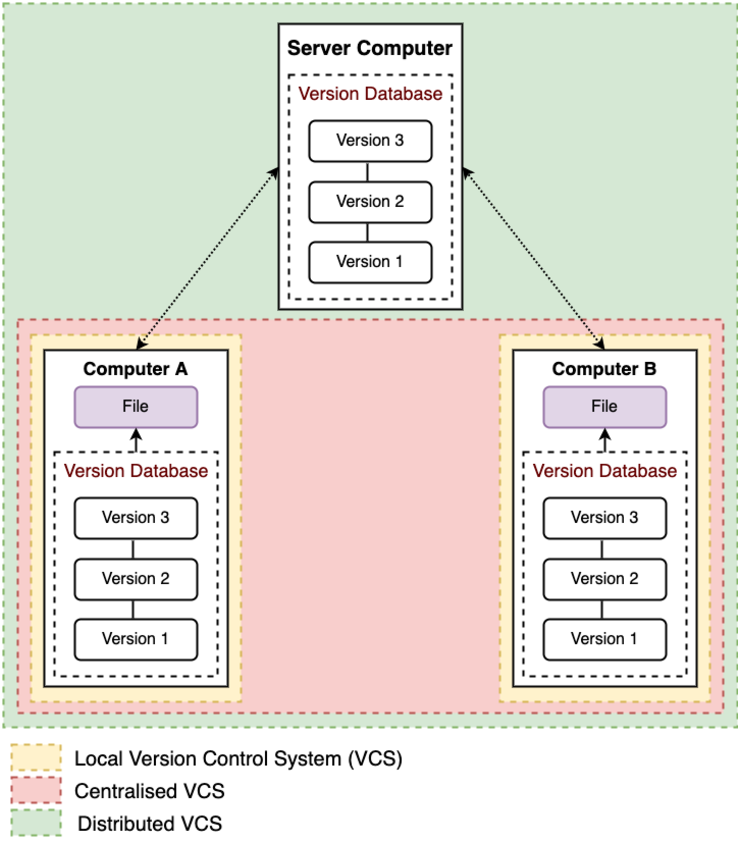
\includegraphics{thesis_files/figure-latex/mf1-1} 

}

\caption[Overview of version control system]{\textbf{Overview of version control system (VCS).} Adapted
from (\protect\hyperlink{ref-chacon2021}{Chacon \& Straub, 2021}).}\label{fig:mf1}
\end{figure}
Programmers developed a local VCS with a database that records all
modifications to the files under revision control to keep track of the
versions. A local VCS is an example of a revision control system (RCS).
Since it is difficult to collaborate with a local VCS, a centralized VCS
was developed, such as Apache Subversion (SVN). All changes to files are
monitored under the centralized server using Centralized VCS. A
centralized VCS, on the other hand, has significant drawbacks. No one
can connect or save versioned changes to something they are working on
if the server goes down for an hour. This leads to the development of
the distributed VCS, such as git. In a distributed VCS, the repository
can be completely mirrored, including the entire version history. A
schematic of distributed VCS is shown in Figure \ref{fig:mf1}, adapted
from (\protect\hyperlink{ref-chacon2021}{Chacon \& Straub, 2021}).

GitHub (\href{https://github.com}{github.com}) a distributed version control
system, was used to manage data analysis projects and software
development projects throughout this doctoral thesis work. One downside
of using GitHub is that files greater than 50 megabytes cannot be
hosted, which means that large files such as sequencing data, FASTQ
files, and BAM files are not version managed. To solve this issue,
git-fat was used, a version-controlled tool that offloads files to a
local directory or another server (\protect\hyperlink{ref-brown2018}{Brown, 2018}).

\hypertarget{m2}{%
\section*{Data analysis directory organization}\label{m2}}
\addcontentsline{toc}{section}{Data analysis directory organization}

ScienceCloud service of the University of Zurich was used for computing.
On ScienceCloud, a data volume is mounted on my instance (virtual
computer). In the data volume, two directories were created, namely
``Data'' and ``Project''. The ``Data'' repository stores raw sequencing files,
FASTQ files, and ``gitfat'' objects, while the Project directory stores
all analysis and code and is version controlled with git. A schematic
representation of this workflow can be seen in Figure \ref{fig:mf2}.
This is done for each dataset analysed.


\begin{figure}[htbp]

{\centering 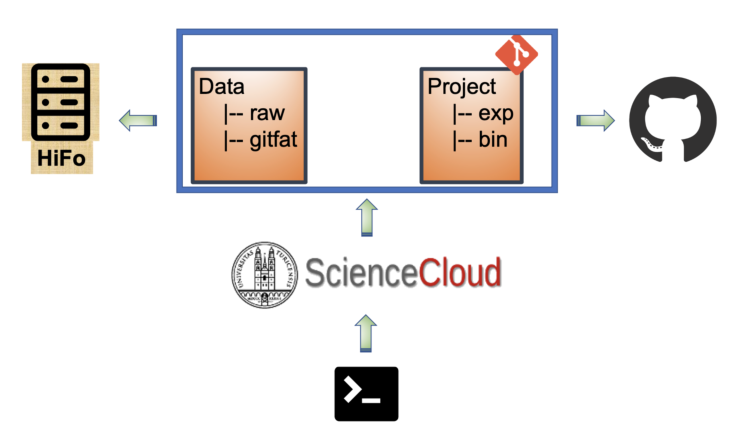
\includegraphics{thesis_files/figure-latex/mf2-1} 

}

\caption[Organization of data analysis projects]{\textbf{Organization of data analysis projects.}}\label{fig:mf2}
\end{figure}
This organization of the data analysis projects ensures open and
reproducible research. As all the analyses are version controlled, one
can look at the analysis conducted back in time. Also, each analysis
script has a log file, which stores the information of the tools version
and any warnings or errors encountered during the analyses. Further, at
the end of the project, the GitHub repository can be made public and all
the code for intermediate data analysis are available to the research
community.

\hypertarget{m3}{%
\section*{Pipelines for data analysis}\label{m3}}
\addcontentsline{toc}{section}{Pipelines for data analysis}

I worked on multi-omics datasets for my doctoral research, which led to
the development of data analysis pipelines for RNA sequencing (RNA-seq),
Assay of Transposase Accessible Chromatin sequencing (ATAC-seq),
Whole-genome bisulfite sequencing (WGBS), Reduced representation
bisulfite sequencing (RRBS), Chromatin immunoprecipitation followed by
sequencing (ChIP-seq), and short RNA sequencing (sRNA-seq).

\hypertarget{m3.1}{%
\subsection*{Quality check and trimming of sequencing datasets}\label{m3.1}}
\addcontentsline{toc}{subsection}{Quality check and trimming of sequencing datasets}

The goal of data quality check and trimming is to find and clean any
data quality issues in the dataset and possibly account for them. The
sequencer determines the nucleotide bases in a DNA or RNA library during
sequencing. A small sequence, known as a read, is created for each
fragment in the library, which is a sequence of nucleotides. In a single
experiment, sequencing technologies, such as Illumina, can generate a
large number of sequence reads. The first step after receiving the
sequenced data is to assess the data quality to determine the
reliability of the sequenced reads. The FASTQ files are examined using
\texttt{FastQC} (\protect\hyperlink{ref-andrews2012}{Andrews et al., 2012}). \texttt{FastQC} provides a comprehensive view of the
data, including the number of sequenced reads, base sequence quality,
``N'' content (if a sequencer cannot call a base, due to the technical
limitations, it enters ``N''; of each sequencing platform.), sequence
duplication levels, and adapter information. A Hypertext Markup Language
(HTML) report generated by the software, for each sample, helps to
understand the pre-processing steps required. The quality assessment is
done using the quality scores (Q-scores) in the FASTQ files, which are
translated to quality statistics in \texttt{FastQC} reports and plotted as
boxplots. Q score is defined as the base-calling error probabilities and
is calculated by the formula: \texttt{**Q\ =\ -log10\ (P)**}. For instance, if a
nucleotide base is assigned a Q score of 30, this is equivalent to the
probability of an incorrect base call of 1/1000 times, which means that
the accuracy of base calling is 99.9\%. A Q score of 30 represents
perfect base calling with no errors and ambiguities and is considered a
benchmark for quality in high-throughput sequencing (HTS) (\protect\hyperlink{ref-ewing1998}{Ewing \& Green, 1998}).

(ref:mfc3)
\textbf{Workflow for quality check and quality control for sequencing data.}
QC: Quality Control.
\begin{figure}[htbp]

{\centering 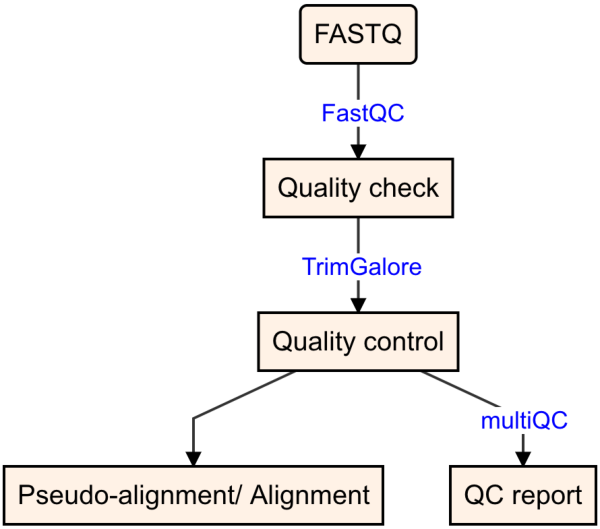
\includegraphics{thesis_files/figure-latex/mf3-1} 

}

\caption[Workflow for quality check and quality control for sequencing data]{(ref:mfc3)}\label{fig:mf3}
\end{figure}
Adaptors are artificial DNA oligonucleotides and are required for
sequencing by platforms like Illumina. During the process of Illumina
library preparation, adaptors are ligated to the short DNA sequences.
Because of the adapters (attached at the end of reads), the sequencing Q
score is usually low, towards the end of the reads. Therefore, these are
required to be removed before downstream processing of the data.
Furthermore, the sequenced DNA reads could have trailing and leading `N'
(if a base caller fails to call a base at a genomic location, it will
put `N' instead of `A', `T', `G' or `C'). Also, there is a chance that
although long reads were sequenced, small reads appeared after
sequencing, or they became shorter after removal of trailing or leading
`N'. It is always better to get rid of small reads below a certain
length, as they would be mapped to multiple locations and will lead to
misinterpretation. Trimming is the process of modifying the ends of
reads. Trimming can help to increase the number of reads that the
aligner or assembler can successfully use, lowering the amount of
unmapped or unassembled reads. \texttt{TrimGalore} is used to trim adapters and
inferior ends of reads with a Phred score of less than 30 (\texttt{-q\ 30}), to
remove Ns from both sides of reads (\texttt{-\/-trim-n}), and to discard trimmed
reads that are too short to be informative (e.g.~\texttt{-\/-length\ 30}, or \texttt{15}
for small RNA-seq data). After this, all results are used to generate an
overview report with \texttt{multiQC} (\protect\hyperlink{ref-ewels2016}{Ewels, Magnusson, Lundin, \& Käller, 2016}), which is a reporting tool
that parses summary statistics from results of other bioinformatics data
analysis tools. Finally, it is critical to recognize, identify, and rule
out issues that may affect downstream analysis interpretation.

The trimmed data is then aligned to the reference genome, indexed with
the specific tool needed for alignment. For example, for aligning WGBS
data with the reference genome, the reference genome is first indexed
with \texttt{Bismark}. This workflow is shown in Figure \ref{fig:mf3}.

Some library preparation kits use the unique molecular identifier (UMI),
which are complex indices and are added to the sequencing libraries
before the polymerase chain reaction (PCR) amplification step. UMIs were
first implemented in the iCLIP protocol (\protect\hyperlink{ref-kuxf6nig2010}{König et al., 2010}) but has been
implemented for RNA-seq, small RNA-seq, single-cell sequencing,
ChIP-seq, and whole-genome sequencing (WGS).

\hypertarget{m3.2}{%
\subsection*{RNA sequencing}\label{m3.2}}
\addcontentsline{toc}{subsection}{RNA sequencing}

RNA sequencing (RNA-seq) is a technique that uses high-throughput
sequencing (HTS) to investigate the quantity and sequences of RNA. It
examines the transcriptome to determine, which of our DNA-encoded genes
are turned on or off, and to what degree. RNA-seq pipeline schematic is
shown in Figure \ref{fig:mf4}.


\begin{figure}[htbp]

{\centering 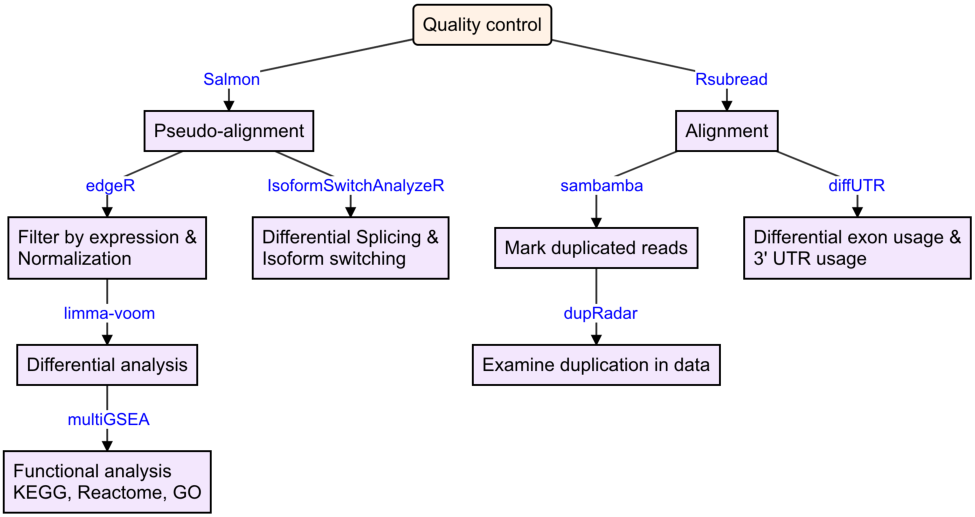
\includegraphics{thesis_files/figure-latex/mf4-1} 

}

\caption[Workflow for RNA sequencing data analysis]{\textbf{Workflow for RNA sequencing data analysis.}}\label{fig:mf4}
\end{figure}
\hypertarget{m3.2.1}{%
\subsubsection*{Pseudo-alignment and alignment}\label{m3.2.1}}
\addcontentsline{toc}{subsubsection}{Pseudo-alignment and alignment}

Sequence alignment is used to determine where the sequences are similar
to the reference genome and how similar they are. We can estimate where
a read came from by aligning or ``mapping'' it to a reference genome or
transcriptome. There are two families of methods for mapping reads in
RNA-seq data: alignment and pseudo-alignment. For alignment, aligners
such as \texttt{STAR} or \texttt{Rsubread} are used. They align reads to a genome or
transcriptome and perform spliced alignment. They return the reads'
base-level alignments. Transcript quantification tools such as \texttt{Salmon}
(\protect\hyperlink{ref-patro2017}{Patro, Duggal, Love, Irizarry, \& Kingsford, 2017}) and \texttt{Kallisto} (\protect\hyperlink{ref-bray2016}{Bray, Pimentel, Melsted, \& Pachter, 2016}) instead perform
pseudo-alignment. These tools use statistical inference to determine
transcript abundances by mapping reads to the transcriptome. Alignments
from the aligners can then be used for a variety of purposes, such as
for feeding transcript assembly tools, for variant calling pipelines, or
for transcript quantification tools.

Quality-controlled reads were pseudo-aligned using \texttt{Salmon} with
automatic detection of the library type (\texttt{-l\ A}), correcting for
sequence-specific bias (\texttt{-\/-seqBias}), and correcting for fragment GC
bias correction (\texttt{-\/-gcBias}) on a \texttt{transcript\ index} prepared from
GENCODE, with additional piRNA precursors and transposable elements
(concatenated by family) from Repeat Masker as in (\protect\hyperlink{ref-gapp2020}{K. Gapp, van Steenwyk, et al., 2020}).
Downstream analyses including differential analysis; differential
transcript usage and differential isoform switching; and functional
analyses, are performed on the pseudo-alignment from \texttt{Salmon}.

Additionally, alignment is performed using the \texttt{Rsubread} package
(\protect\hyperlink{ref-liao2019}{Liao, Smyth, \& Shi, 2019}) using the \texttt{subjunc()} function, specific for RNA-seq data.
Analysis of duplicates, differential exon usage, and differential 3'
usage are performed on alignment obtained from \texttt{Rsubread}.

A direct comparison of genome alignment with transcriptome
pseudo-alignment was performed in (\protect\hyperlink{ref-yi2018}{Yi, Liu, Melsted, \& Pachter, 2018}) and the authors found that
both approaches produce similar quantifications. However, (\protect\hyperlink{ref-wu2018}{D. C. Wu, Yao, Ho, Lambowitz, \& Wilke, 2018})
suggested that it is not optimal to use alignment-free methods to
analyze and quantify lowly expressed genes and small RNAs.

\hypertarget{m3.2.2}{%
\subsubsection*{Duplicated reads analysis}\label{m3.2.2}}
\addcontentsline{toc}{subsubsection}{Duplicated reads analysis}

Duplicated reads are different copies of the exact same sequence. Unless
a genomic region is highly expressed, most mRNA fragments are expected
to be unique. A low degree of repetition may indicate that the target
sequence is well-covered, whereas a high level of duplication is more
likely to signal bias. Duplicate reads might be caused by PCR
duplication or legitimately overrepresented sequences. Because PCR
amplification is more efficient for some sequences than others, it can
misrepresent the true proportion of sequences in the input, whereas
truly overrepresented sequences are the result of very abundant
transcripts in an RNA-Seq library and are an expected case and not of
concern because they accurately represent the input.

Throughout the research, duplicated reads were marked in the aligned
data using \texttt{sambamba} (\protect\hyperlink{ref-tarasov2015}{Tarasov, Vilella, Cuppen, Nijman, \& Prins, 2015}), and further, the quality issues
with PCR duplicates are analyzed using \texttt{dupRadar} (\protect\hyperlink{ref-sayols2016}{Sayols, Scherzinger, \& Klein, 2016}).
\texttt{dupRadar} aids in separating the fraction of readings produced by
artefacts from the fraction resulting from high expression.

\hypertarget{m3.2.3}{%
\subsubsection*{Differential expression analysis}\label{m3.2.3}}
\addcontentsline{toc}{subsubsection}{Differential expression analysis}

Differential expression analysis (at the transcript or gene level) is
the statistical examination of normalised read count data to find
quantitative differences in expression levels between experimental
groups.

Read counts at the transcript level are obtained from pseudo-aligned
data and are aggregated at the gene level. Low counts of candidate
genes/transcripts across samples give minimal evidence for differential
expression. When evaluating false discovery rates, they also add to the
multiple testing burden, lowering the ability to find differentially
expressed genes. A pre-filtering of counts is therefore performed using
the \texttt{filterByExpr()} function from \texttt{edgeR} (\protect\hyperlink{ref-robinson2010}{Robinson, McCarthy, \& Smyth, 2010a}) with a design
matrix (matrix containing data about multiple characteristics of several
samples, such as biological group, age, and batch for library
preparation) and requiring at least 20 counts (min.counts = 20)
(\protect\hyperlink{ref-germain2020}{Germain, Sonrel, \& Robinson, 2020}). Next, the counts are normalized for different sequencing
depths between samples and to eliminate composition biases between
samples, for example, if there are a few highly expressed genes
dominating in some samples, leading to fewer reads from other genes.
Normalization factors are obtained using the \texttt{TMM} normalization method
(\protect\hyperlink{ref-robinson2010}{Robinson et al., 2010a}) from the \texttt{edgeR} package, using the calcNormFactors
function. \texttt{TMM} stands for Trimmed Mean of M values, in which the counts
for the samples are scaled using a weighted trimmed mean of the log
expression ratios. Differential expression analysis at gene and
transcript level is performed using limma-voom (\protect\hyperlink{ref-law2014}{C. W. Law, Chen, Shi, \& Smyth, 2014}) pipeline from
limma (\protect\hyperlink{ref-ritchie2015}{Ritchie et al., 2015}) package.

\hypertarget{m3.2.4}{%
\subsubsection*{Exploratory data analysis}\label{m3.2.4}}
\addcontentsline{toc}{subsubsection}{Exploratory data analysis}

Exploratory data analysis of counts (using principal component analysis,
PCA), differential analysis results (volcano plot, MA plot, and
heatmap), and assessment of library composition is performed using
\texttt{plgINS}, a versatile \texttt{R} package,
(\href{https://github.com/ETHZ-INS/plgINS}{github.com/ETHZ-INS/plgINS}),
under development by Dr.~Pierre-Luc Germain. The package also comes with
a shiny application.

\hypertarget{m3.2.5}{%
\subsubsection*{Differential transcript usage and differential isoform switching}\label{m3.2.5}}
\addcontentsline{toc}{subsubsection}{Differential transcript usage and differential isoform switching}

Differential transcript usage (DTU) analysis looks for proportional
differences in the makeup of a gene's transcripts between conditions.

DTU is performed using \texttt{IsoformSwitchAnalyzeR} (\protect\hyperlink{ref-vitting-seerup2017}{Vitting-Seerup \& Sandelin, 2017}, \protect\hyperlink{ref-vitting-seerup2019}{2019}). Isoforms are annotated via integration of a wide
range of (predicted) annotations: Pfam was used for prediction of
protein domains, CPC2 (version 2.0) for calculation of the coding
potential, SignalP (version 5.0) for prediction of Signal Peptides, and
IUPred2A was used to predict Intrinsically Disordered Region (IDRs) and
Intrinsically Disordered Binding Regions (IDBRs). The results from Pfam,
CPC2, IUPred2A, and SignalP are used with \texttt{IsoformSwitchAnalyzeR} for
annotation and prediction of functional consequences for the identified
isoform changes.

\hypertarget{m3.2.6}{%
\subsubsection*{Differential exon usage and differential 3' untranslated regions usage}\label{m3.2.6}}
\addcontentsline{toc}{subsubsection}{Differential exon usage and differential 3' untranslated regions usage}

Differential exon usage (DEU) analysis looks for variations in exon
usage between experimental conditions. mRNAs' 3' untranslated regions
(3' UTRs) are best recognized for regulating mRNA-based functions such
as mRNA localization, stability, and translation (\protect\hyperlink{ref-mayr2019}{Mayr, 2019}).
Differential UTR usage looks for variations in 3' UTR usage between
experimental conditions.

DEU and differential 3' UTR usage are performed using the diffUTR R
package (\protect\hyperlink{ref-gerber2021}{Gerber, Schratt, \& Germain, 2021}).

\hypertarget{m3.2.7}{%
\subsubsection*{Functional analysis}\label{m3.2.7}}
\addcontentsline{toc}{subsubsection}{Functional analysis}

The output of RNA-seq differential expression analysis is a list of
significant differentially expressed genes (DEGs). The goal of
functional analysis is to provide biological insight of DEGs. Functional
analysis on Kyoto Encyclopedia of Genes and Genomes (KEGG)
(\protect\hyperlink{ref-kanehisa2021}{Kanehisa, Furumichi, Sato, Ishiguro-Watanabe, \& Tanabe, 2021}), Reactome (\protect\hyperlink{ref-jassal2020}{Jassal et al., 2020}), Gene Ontology (GO)
(\protect\hyperlink{ref-consortium2021}{Consortium, 2021}) and curated pathway list from the Gene Set Enrichment
Analysis (GSEA) (\protect\hyperlink{ref-subramanian2005}{Subramanian et al., 2005}) databases is performed using
multiGSEA
(\href{https://github.com/lianos/multiGSEA}{github.com/lianos/multiGSEA}),
which facilitates the analysis with GOseq (\protect\hyperlink{ref-young2010}{Young, Wakefield, Smyth, \& Oshlack, 2010}), fGSEA
(\protect\hyperlink{ref-korotkevich2016}{Korotkevich et al., 2016}), Correlation Adjusted MEan RAnk gene set test
(CAMERA) and camera pre-ranked (CAMERA-PR) (\protect\hyperlink{ref-wu2012}{D. Wu \& Smyth, 2012}), ROtation testing
using MEan Ranks (ROMER) and fry (\protect\hyperlink{ref-ritchie2015}{Ritchie et al., 2015}), and ROtAtion gene Set
Testing (ROAST) (\protect\hyperlink{ref-wu2010}{D. Wu et al., 2010}). An advantage of using multiGSEA is that it
has standardized input and output and provides a Shiny app for
exploratory data analysis
(\href{https://github.com/lianos/multiGSEA.shiny}{github.com/lianos/multiGSEA.shiny}).
With multiGSEA, it is easy to specify to use testing relative to a
threshold (TREAT) method (\protect\hyperlink{ref-mccarthy2009}{McCarthy \& Smyth, 2009}), which takes a user-specified
log fold change cut-off and recalculates the moderated t-statistics and
p-values. Using TREAT only affects enrichment tests that first threshold
the genes in the experiment as ``significant'' or not, like GOseq and not
tests like the camera.

\hypertarget{m3.3}{%
\subsection*{Assay of Transposase Accessible Chromatin sequencing}\label{m3.3}}
\addcontentsline{toc}{subsection}{Assay of Transposase Accessible Chromatin sequencing}

The Assay of Transposase Accessible Chromatin sequencing (ATAC-seq) is
widely used in studying chromatin biology to study chromatin
accessibility and to identify open chromatin regions (OCRs). The
nucleosome is the most basic component of chromatin. Each nucleosome is
made up of about two turns of DNA wrapped around a set of eight proteins
called histones known as histone octamer. With the help of nucleosomes,
the genome is securely packed and structured, known as chromatin. The
organization and accessibility of DNA are influenced by a number of
factors, including chromatin structure, nucleosome location,
transcription factors, and histone modifications. As a result, these
factors have a role in the activation and inactivation of genes. The
genome is treated with a hyperactive version of the Tn5 transposase to
insert sequencing adapters into OCRs (\protect\hyperlink{ref-buenrostro2015}{Buenrostro, Wu, Chang, \& Greenleaf, 2015}). Because it is
easier, faster, and uses fewer cells than competing approaches like
FAIRE-Seq and DNase-Seq, ATAC-Seq has become popular for discovering
accessible regions of the genome. The schematic of the ATAC-seq pipeline
is shown in Figure \ref{fig:mf5}.



\begin{figure}[htbp]

{\centering 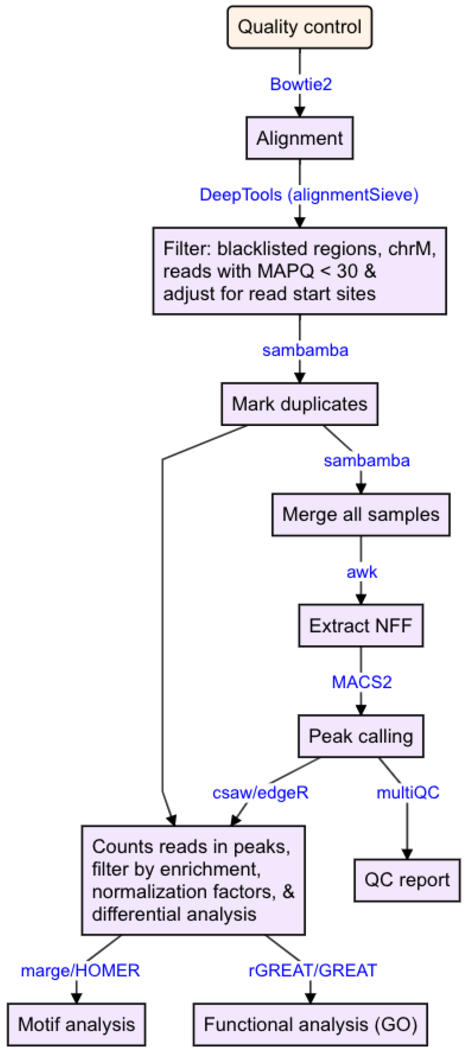
\includegraphics{thesis_files/figure-latex/mf5-1} 

}

\caption[Workflow for ATAC sequencing data analysis]{\textbf{Workflow for ATAC sequencing data analysis.} QC:
Quality Control, NFF: Nucleosome Free Fragments.}\label{fig:mf5}
\end{figure}
\hypertarget{m3.3.1}{%
\subsubsection*{Alignment, post-alignment quality control, and peak calling}\label{m3.3.1}}
\addcontentsline{toc}{subsubsection}{Alignment, post-alignment quality control, and peak calling}

Alignment of the ATAC-seq data is performed using \texttt{Bowtie2}
(\protect\hyperlink{ref-langmead2012}{Langmead \& Salzberg, 2012}) with the following parameters: fragments up to 2 kb were
allowed to align (-X 2000), entire read alignment (--end-to-end),
suppressing unpaired alignments for paired reads (--no-mixed),
suppressing discordant alignments for paired reads (--no-discordant) and
minimum acceptable alignment score with respect to the read length
(--score-min L,-0.4,-0.4). Tn5 inserts adapters separated by 9bp when it
cuts an accessible chromatin region (\protect\hyperlink{ref-kia2017}{Kia et al., 2017}). This indicates that
reads on the positive strand should be adjusted 4 bp to the right and
reads on the negative strands should be shifted 5 bp to the left in
order for the read start site to reflect the centre of where Tn5 binds
as done in (\protect\hyperlink{ref-buenrostro2013}{Buenrostro, Giresi, Zaba, Chang, \& Greenleaf, 2013}), which is important for the footprint
analysis. Using alignmentSieve from deepTools (\protect\hyperlink{ref-ramirez2016}{Ramirez et al., 2016}), aligned
data (BAM files) are adjusted for the read start sites to represent the
centre of the transposon cutting event (--ATACshift), and filtered for
reads with a high mapping quality (--minMappingQuality 30). In addition,
because the mitochondrial genome is devoid of chromatin packaging
(\protect\hyperlink{ref-bogenhagen2012}{Bogenhagen, 2012}) a large number of mitochondrial reads can be a concern
in ATAC-seq. Some ATAC-Seq samples have been found to include 80\%
mitochondrial reads, prompting the development of wet-lab approaches to
address the problem (\protect\hyperlink{ref-corces2017}{Corces et al., 2017}). Also, because the open chromatin
regions of interest are typically found in the nuclear genome,
mitochondrial reads are typically excluded from the analysis. Hence,
reads mapping to the mitochondrial chromosome and ENCODE blacklisted
regions (regions where genome assembly results in erroneous signal) were
filtered using alignmentSieve. Because ATAC-seq does not require
rigorous size selection during library preparation, it can identify
nucleosome positions using fragments representing nucleosome-free
fragments (NFFs) nucleosome monomers, and multimers. There is
approximately 147 bp of DNA wrapped around a nucleosome, and in order to
obtain NFFs, which are indicative of transcription factor bindings, the
fragments less than 147 bp must be extracted. To extract NFFs, all
aligned files are merged within experimental groups, reads are sorted by
left-most coordinates and indexed using SAMtools (\protect\hyperlink{ref-li2009}{H. Li et al., 2009}), and NFFs
were obtained by selecting alignments with a template length between 40
and 140 inclusively (\protect\hyperlink{ref-goodnight2019}{Goodnight et al., 2019}; \protect\hyperlink{ref-jung2017}{Jung et al., 2017}). Peak calling is a
statistical approach that leverages data coverage properties to identify
locations that are enriched as a result of protein/ transcription factor
binding. To find regions corresponding to potential OCRs in the
nucleosome-free regions, we want to identify regions where reads have
piled up greater than the background read coverage. Peak calling on the
NFFs is performed using MACS2 (\protect\hyperlink{ref-zhang2008}{Yong Zhang et al., 2008}) with genome size in base-pair
(-g genomeSize) and specifying the paired-end BAM file format (-f
BAMPE).

\hypertarget{m3.3.2}{%
\subsubsection*{Peaks annotation and differential accessibility analysis}\label{m3.3.2}}
\addcontentsline{toc}{subsubsection}{Peaks annotation and differential accessibility analysis}

The goal of peak annotation is to map peaks to the regulatory elements.
The peaks are annotated with transcript, and the distance to the nearest
transcription start site, based on overlap with gene transfer format
(GTF) file obtained from the GENCODE. The number of extended reads
overlapping in the peak regions is calculated using the csaw package
(\protect\hyperlink{ref-lun2015}{Lun \& Smyth, 2015}). Peak regions that did not have at least 15 reads in at least
40\% of the samples were filtered out. Normalization factors were
obtained on the filtered peak regions using the \texttt{TMM} normalization
method (\protect\hyperlink{ref-robinson2010}{Robinson et al., 2010a}) and differential accessibility analysis is
performed using the Genewise Negative Binomial Generalized Linear Models
with Quasi-likelihood (glmQLFit) test from the \texttt{edgeR} package. \texttt{edgeR}
has recently been benchmarked and recommended for differential chromatin
accessibility analysis (\protect\hyperlink{ref-gontarz2020}{Gontarz et al., 2020}).

\hypertarget{m3.3.3}{%
\subsubsection*{Functional analysis}\label{m3.3.3}}
\addcontentsline{toc}{subsubsection}{Functional analysis}

GO analysis is performed on differentially accessible regions (DARs)
with the rGREAT package
(\href{https://github.com/jokergoo/rGREAT}{github.com/jokergoo/rGREAT}),
which is a wrapper around the Genomic Regions Enrichment of Annotations
Tool (GREAT) (\protect\hyperlink{ref-mclean2010}{McLean et al., 2010}). Transcription factor motif enrichment
analysis is performed using the marge package (\protect\hyperlink{ref-amezquita2018}{Amezquita, 2018}), which is
a wrapper around the Homer tool (\protect\hyperlink{ref-heinz2010}{Heinz et al., 2010}).

\hypertarget{m3.3.4}{%
\subsubsection*{Differential accessibility analysis at transposable elements}\label{m3.3.4}}
\addcontentsline{toc}{subsubsection}{Differential accessibility analysis at transposable elements}

Transposable elements (TEs) GTF file is obtained from
\href{http://labshare.cshl.edu/shares/mhammelllab/www-data/TEtranscripts/TE_GTF/mm10_rmsk_TE.gtf.gz\%20on\%2003.02.2020}{http://labshare.cshl.edu/shares/mhammelllab/www-data/TEtranscripts/TE\_GTF/mm10\_rmsk\_TE.gtf.gz}.
The GTF file provides hierarchical information about TEs: \textbf{Class}
(level 1, eg. LTR), \textbf{Family} (level 2, eg. LTR L1), \textbf{Subtype} (level
3, eg. LTR L1 L1\_Rod), and \textbf{Locus} (level 4, eg. LTR L1 L1\_Rod
L1\_Rod\_dup1). TE loci are annotated based on overlap with GENCODE as
described above for ATAC-seq peaks. Filtered BAM files (without reads
mapping to blacklisted or mitochondrial regions) are used for analyzing
TEs. Mapped reads are assigned to TEs using featureCounts from the R
package \texttt{Rsubread} (\protect\hyperlink{ref-liao2019}{Liao et al., 2019}) and were summarized to Subtypes (level
3), allowing for multi-overlap with fractional counts, while ignoring
duplicates. The number of extended reads overlapping at the TE loci is
obtained using the csaw package (\protect\hyperlink{ref-lun2015}{Lun \& Smyth, 2015}). Subtypes that did not have
at least 15 reads, and loci that did not have at least 5 reads in at
least 40\% of the samples, were filtered out. Normalization and
differential accessibility analysis is performed as described above for
the peaks. GO and motif enrichment analysis is performed as described
above for the peak regions.

\hypertarget{m3.4}{%
\subsection*{Chromatin immunoprecipitation followed by sequencing}\label{m3.4}}
\addcontentsline{toc}{subsection}{Chromatin immunoprecipitation followed by sequencing}

A substantial part of gene expression regulation is controlled by
protein-DNA interactions. Proteins like transcription factors and
histones influence how much and where genes are expressed. ChIP,
followed by sequencing, can be used to investigate the interaction
between a DNA sequence and a protein. There are two types of ChIP:
cross-linked ChIP (X-ChIP) and native ChIP (N-ChIP). Formaldehyde is
utilized to crosslink histones to DNA, and ultrasound sonication is used
to fragment the DNA in X-ChIP, whereas the native covalent interaction
between protein and DNA is exploited in N-ChIP (\protect\hyperlink{ref-park2009}{Park, 2009}). The
fundamental purpose of ChIP is to map global binding sites for any
protein of interest, such as transcription factors (TF) and histones, in
order to investigate specific modifications. In vivo, the approach
generates a library of DNA locations bound to the protein of interest.
Following ChIP on samples, library preparation, PCR amplification, and
ultimately deep sequencing are performed. The schematic of the ChIP-seq
pipeline is shown in Figure \ref{fig:mf6}.



\begin{figure}[htbp]

{\centering 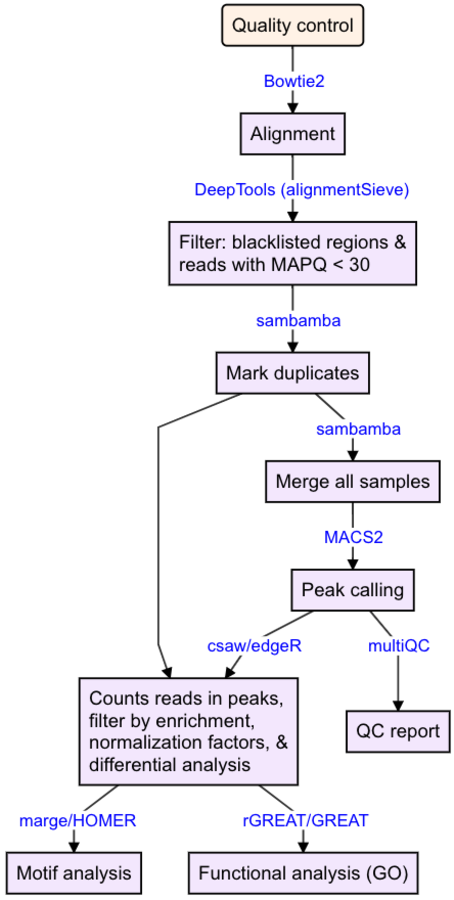
\includegraphics{thesis_files/figure-latex/mf6-1} 

}

\caption[Workflow for ChIP sequencing data analysis]{\textbf{Workflow for ChIP sequencing data analysis.} QC:
Quality Control.}\label{fig:mf6}
\end{figure}
\hypertarget{m3.4.1}{%
\subsubsection*{Alignment and peak calling}\label{m3.4.1}}
\addcontentsline{toc}{subsubsection}{Alignment and peak calling}

Alignment is performed using \texttt{Bowtie2}. Reads with more than 3
mismatches are removed from the aligned data, as suggested in
(\protect\hyperlink{ref-royo2016}{Royo, Stadler, \& Peters, 2016}), and reads with low mapping quality (--minMappingQuality 30)
or mapping to the mitochondrial chromosome or aforementioned blacklisted
regions are also filtered out. Peak calling is performed using MACS2
with mouse genome size in base-pair (-g genomeSize) and the BAM file
format (-f BAM/PEBAM), together with the ChIP input sample.

\hypertarget{m3.4.2}{%
\subsubsection*{Peaks annotation, differential analysis, and functional analysis}\label{m3.4.2}}
\addcontentsline{toc}{subsubsection}{Peaks annotation, differential analysis, and functional analysis}

These analyses are performed as described above for the ATAC-seq peaks.

\hypertarget{m3.5}{%
\subsection*{Bisulfite sequencing}\label{m3.5}}
\addcontentsline{toc}{subsection}{Bisulfite sequencing}

DNA methylation (DNAme) involves the addition of methyl groups to the
DNA molecule. It most normally occurs at the C5 position of cytosines
inside CpG dinucleotides, where it is stable during mitosis and meiosis.
Methylation can change the activity of DNA without changing its
sequence. DNAme is a reversible, cell-type-specific DNA modification
that is usually persistent through cell division. It is not equally
distributed across the genome, but rather is linked to CpG density.
High-throughput bisulfite sequencing is one of the most reliable methods
for measuring DNA methylation. In bisulfite conversion, unmethylated
cytosine residues are converted to uracil, but methylated cytosines
remain intact (\protect\hyperlink{ref-frommer1992}{Frommer et al., 1992}), allowing methylation and unmethylated
cytosine bases to be distinguished. Following PCR amplification, these
uracils are converted to thymines. This is followed by the WGBS. WGBS is
considered a gold-standard technology for DNA methylation detection as
it provides a qualitative, quantitative, and efficient technique to
identify 5-methylcytosine at single base-pair resolution. The cost of
sequencing an entire genome is typically quite high. As a result,
despite its use on huge genomes like the human genome, significant
numbers of individual samples are rarely sequenced. For this reason,
RRBS was developed, in which the bisulfite process occurs but only
around 1\% of the genome is sequenced. This makes it possible to sequence
the genomes in greater numbers. The idea behind RRBS is to enrich the
sequencing library with CpG-dense sections of the genome to boost the
sequencing depth of cytosine-rich areas (\protect\hyperlink{ref-meissner2005}{Meissner et al., 2005}). This is done by
using CpG-specific restriction enzymes like MspI, which identifies the
sequence 5'-CCGG-3'. MspI cleaves the complete genome in RRBS, leaving
at least two cytosines per cleaved DNA fragment (one cytosine at either
end of the MspI-MspI fragment). Sequencing libraries are made from
size-selected MspI DNA fragments, followed by bisulfite conversion and
sequencing of the converted library. The schematic of the BS-seq
pipeline is shown in Figure \ref{fig:mf6}.




\begin{figure}[htbp]

{\centering 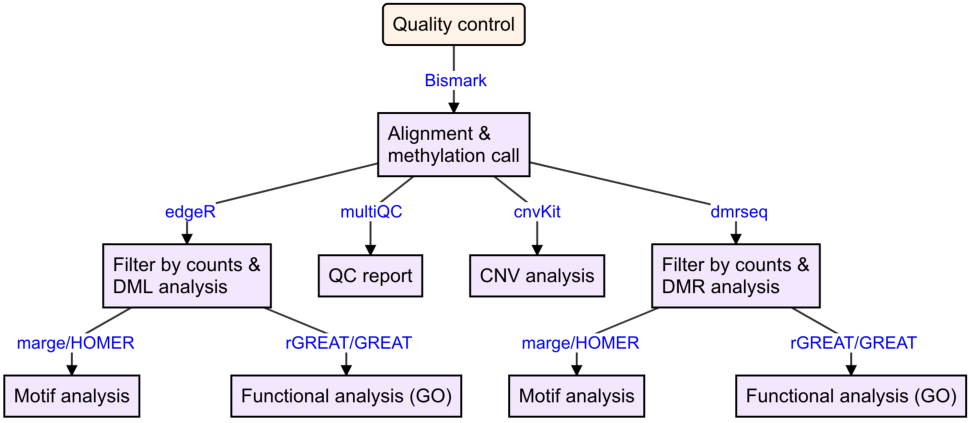
\includegraphics{thesis_files/figure-latex/mf7-1} 

}

\caption[Workflow for Bisulfite sequencing data analysis]{\textbf{Workflow for Bisulfite sequencing data analysis.} QC:
Quality Control, DML: differentially methylated loci, DMR:
differentially methylated regions, CNV: copy-number variation.}\label{fig:mf7}
\end{figure}
\hypertarget{m3.5.1}{%
\subsubsection*{Alignment and methylation calling}\label{m3.5.1}}
\addcontentsline{toc}{subsubsection}{Alignment and methylation calling}

Mismatches between the reads and the reference genome are introduced
during bisulfite conversion, resulting in slow and imprecise mapping.
Further, the DNA code's complexity is reduced. Hence, specialized tools
are required for aligning the bisulfite sequencing data. Alignment of
the bisulfite sequencing data is performed using \texttt{Bismark}
(\protect\hyperlink{ref-krueger2011}{Krueger \& Andrews, 2011}) on a genome index built using
\texttt{Bismark}\_genome\_preparation. Methylation information for individual
cytosines (methylation calls) is extracted using the
\texttt{Bismark}\_methylation\_extractor tool from the \texttt{Bismark} package.

\hypertarget{m3.5.2}{%
\subsubsection*{Differential methylation analysis}\label{m3.5.2}}
\addcontentsline{toc}{subsubsection}{Differential methylation analysis}

Differential analysis can be performed at the loci level (differentially
methylated loci, DML) or at the region's level (differentially
methylated regions, DMRs). For the identification of DML and DMRs, the
data is first filtered by the coverage among samples. DML are identified
using \texttt{edgeR}. Identification of DMRs is not so straightforward, as
defining regions boundaries is not easy the tool has to take into
account correlation across loci of a region. Hence, during a course, we
benchmarked different tools for detecting DMRs
\href{https://dktanwar.github.io/sta426-project-dmr-comparison/report/project_report.html}{dktanwar.github.io/sta426-project-dmr-comparison}
and found dmrseq to outperform all other methods that we compared. DMRs
from RRBS data are identified using the parameters recommended by Dr.
Keegan Korthauer\textbf{,} author of dmrseq
(\href{https://github.com/kdkorthauer/dmrseq/issues/14}{github.com/kdkorthauer/dmrseq/issues/14}).

\hypertarget{m3.5.3}{%
\subsubsection*{Copy number variation analysis}\label{m3.5.3}}
\addcontentsline{toc}{subsubsection}{Copy number variation analysis}

The phenomenon of copy number variation (CNV) occurs when regions of the
genome are repeated and the amount of repeats differs between
individuals. CNV is a type of structural variation that occurs when a
duplication or deletion event occurs that impacts a large number of base
pairs. To infer and visualize CNV from WGBS data, we use the CNVkit
(\protect\hyperlink{ref-talevich2016}{Talevich, Shain, Botton, \& Bastian, 2016}).

\hypertarget{m3.5.4}{%
\subsubsection*{DML and DMR annotation, and functional analysis}\label{m3.5.4}}
\addcontentsline{toc}{subsubsection}{DML and DMR annotation, and functional analysis}

These analyses are performed as described above for the ATAC-seq data.

\hypertarget{m3.6}{%
\subsection*{Short RNA-seq}\label{m3.6}}
\addcontentsline{toc}{subsection}{Short RNA-seq}

The short RNA-seq pipeline is not described in this section, as a method
for analyzing small RNA-seq data has been developed and is discussed in
detail in Chapter 3.

\hypertarget{m3.7}{%
\subsection*{Multi-omics analysis}\label{m3.7}}
\addcontentsline{toc}{subsection}{Multi-omics analysis}

Using different experiments, followed by sequencing, on the same samples
or cells/tissues, such as RNA-seq, ATAC-seq, ChIP-seq, and BS-seq,
results in multi-dimensional omics datasets that can be used to
investigate relationships between different biological processes, such
as gene expression, chromatin accessibility, histone modifications, and
DNA methylation. Integrating multi-omics datasets is most challenging
and is not straightforward to perform, as there are no standard recipes.

We present a straightforward and biologically useful approach for
performing multi-omics analysis on RNA-seq, ATAC-seq, ChIP-seq, and
BS-seq datasets. First, we overlap the DARs with ChIP-seq peaks
enrichment, RNA-seq expression of overlapping genes with DARs, and
methylation values of DARs overlapping loci from BS-seq data into one
matrix, overlapMatrix. The DARs are initially divided into proximal
(less than +/- 2.5 kb from a TSS) and distal (more than +/- 2.5 kb from
a TSS) regions, as per the ENCODE guidelines (\protect\hyperlink{ref-harrow2012}{Harrow et al., 2012}; \protect\hyperlink{ref-thurman2012}{Thurman et al., 2012}); the proximal regions are further divided into active and
inactive (proximal active and proximal inactive) groups based on nearby
gene expression (if nearby gene expression is detected) (\textbf{step 1}).
Next, these three groups are separated based on whether the biological
groups are more or less accessible (\textbf{step 2}). This classification
would reveal six separate clusters of DARs, each with its own biological
profile. Further, proximally active genes are categorised based on their
up/ down expression (\textbf{step 3}). Moreover, we categorised DARs
depending on whether they had H3K4me3, which is a critical marker for
the active transcription and developmentally stable genes (\protect\hyperlink{ref-fu2019}{L. Fu \& Zhang, 2019});
H3K27ac, which is associated with the higher activation of transcription
and therefore defined as an active enhancer mark (\protect\hyperlink{ref-zhang2020}{T. Zhang, Zhang, Dong, Xiong, \& Zhu, 2020}); or dual
H3K4me3/H3K27ac enrichment (\protect\hyperlink{ref-beacon2021}{Beacon et al., 2021}); as well as H3K27me3
enrichment, which is involved in transcriptional silencing
(\protect\hyperlink{ref-bogliotti2012}{Bogliotti \& Ross, 2012}) (\textbf{step 4}). The schematic is shown in Figure
\ref{fig:mf8}. Furthermore, gene ontology and TF motif enrichment
analysis can be done on these categorised DARs. For a more in-depth
understanding, all of the regions can be further classified based on
their methylation state (high or low). Please see \protect\hyperlink{chapter2}{Chapter 2}
for an application of this multi-omics analysis.

\newpage
\begin{landscape}


\begin{figure}[htbp]

{\centering 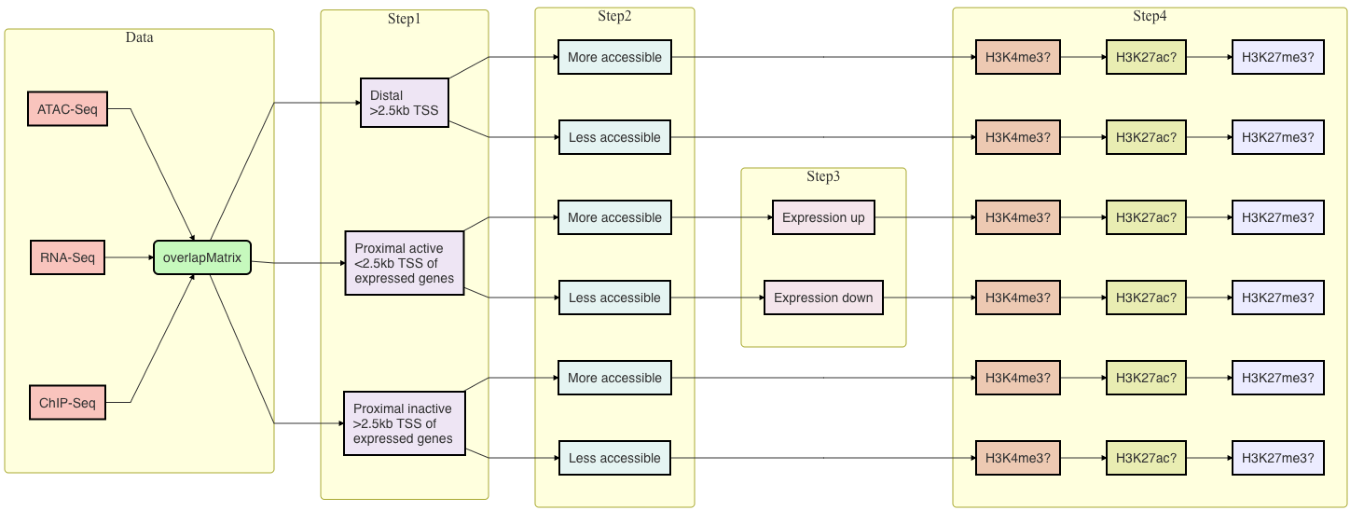
\includegraphics{thesis_files/figure-latex/mf8-1} 

}

\caption[Workflow for multi-omics data integration]{\textbf{Workflow for multi-omics data integration.}}\label{fig:mf8}
\end{figure}
\end{landscape}
Visualization of these regions is an essential step. We used
EnrichedHeatmap (\protect\hyperlink{ref-gu2018}{Gu, Eils, Schlesner, \& Ishaque, 2018}) and ComplexHeatmap (\protect\hyperlink{ref-gu2016}{Gu, Eils, \& Schlesner, 2016a}) packages for the
visualization of categorized DARs.

\textbf{ATAC-seq:} ATAC-seq data is the starting point and we first find the
middle of each DARs. After that, we obtain the coverage for 1kb upstream
and downstream from the middle of DARs. We use the \texttt{normalizeToMatrix}
function from the EnrichedHeatmap package and normalized the signal
using the weighted mean between the intersected parts and un-intersected
parts(mean\_mode = ``w0'') in a window of 50bp. In the normalized matrix,
each row corresponds to DAR and each column corresponds to a window
either on upstream or downstream of middle of the peak.

\[
v_{w 0}=\frac{\sum_{i=1}^{n} x_{i} w_{i}}{W+W^{\prime}}
\]

\({W}\) is the sum of width of the intersected parts
\(\left(\sum_{i}^{n} w_{i}\right)\) and \(W^{\prime}\) is the sum of width
for the non-intersected parts.

For visualization, DARs are ordered by the enriched scores. For each DAR
in the matrix, values are denoted as \({x}\), indices as
\(1, \ldots, n_{1}\) for upstream windows, indices as \(n_{1}+1, \ldots, n\)
for downstream windows, and \(n_{2}=n-n_{1}\) are the enriched score that
are calculated as the sum of \({x}\) weighted by distance to middle of the
peak. DAR has a higher enriched score when there is more signal focused
on it.

\[
\sum_{i=1}^{n_{1}} x_{i} \cdot i / n_{1}+\sum_{i=n_{1}+1}^{n} x_{i} \cdot(n-i+1) / n_{2}
\]

Moreover, we also plot the log\textsubscript[2{]}fold-changes of DARs using
ComplexHeatmap.

\textbf{ChIP-seq:} ChIP-seq data coverage for 1kb upstream and downstream
from the mid of DARs is obtained. We use the \texttt{normalizeToMatrix} function
from the EnrichedHeatmap package and normalized the signal using the
weighted mean between the intersected parts and un-intersected parts
(mean\_mode = ``w0'') in a window of 50bp.

\textbf{BS-seq:} BS-seq data methylation values for 1kb upstream and
downstream from the mid of DARs is obtained. We use the
\texttt{normalizeToMatrix} function from the EnrichedHeatmap package and
normalized the signal using the mean of all the signals (mean\_mode =
``absolute'') in a window of 50bp.

\[
v_{a}=\frac{\sum_{i=1}^{n} x_{i}}{n}
\]

\textbf{RNA-seq:} For RNA-seq data, we used ComplexHeatmap to plot the
log\textsubscript[2{]}-fold-changes of expression values between the groups, and also the
log\textsubscript[2{]}-fold-changes obtained after the differential analysis.

\hypertarget{chapter1}{%
\chapter{Dynamic chromatin accessibility in spermatogonial cells for transcriptional programmings from early postnatal to adult stages}\label{chapter1}}

\textbf{Deepak K Tanwar}\textsuperscript{1,2,3,$\dagger$}, Irina
Lazar-Contes\textsuperscript{1,2,3,$\dagger$}, Pierre-Luc
Germain\textsuperscript{1,2,3,4}, Isabelle M
Mansuy\textsuperscript{1,2,3,\#}\newline \newline
\textsuperscript{1}Laboratory of Neuroepigenetics, Brain Research
Institute at the Medical Faculty of the University of Zurich. \newline
\textsuperscript{2}Institute for Neuroscience of the Department of
Health Sciences and Technology, ETH Zurich, Zurich, Switzerland.\newline
\textsuperscript{3}Zurich Neuroscience Center, ETH and University of
Zurich, Zurich, Switzerland. \newline \textsuperscript{4}Statistical
Bioinformatics Group, Swiss Institute of Bioinformatics, Zurich,
Switzerland. \newline \newline \textsuperscript{$\dagger$}Equal
contributions \newline\newline \textsuperscript{\#}Corresponding
author \newline\newline 
\textbf{Contributions:} \emph{I performed data analysis, generated figures, wrote computational methods and figure captions, revised manuscript.}

\newpage

\hypertarget{update-on-the-new-data-analysis}{%
\section{Update on the new data analysis}\label{update-on-the-new-data-analysis}}

This project has undergone two major changes as a result of the
replacement of one of the spermatogonial cells (SCs) RNA-seq datasets by
a better one.

\hypertarget{code-availibility}{%
\subsection{Code availibility}\label{code-availibility}}
\begin{itemize}
\item
  BioRxiv version:
  \href{https://github.com/mansuylab/SC_postnatal_adult/tree/bioRxiv_v1}{bioRxiv\_v1}
\item
  This thesis version:
  \href{https://github.com/mansuylab/SC_postnatal_adult/tree/thesis_manuscript}{thesis\_manuscript}
\item
  New analysis after inclusion of new RNA-seq data:
  \href{https://github.com/mansuylab/SC_postnatal_adult/tree/deepak}{deepak}
\end{itemize}
\hypertarget{inclusion-of-rna-seq-data-from-the-literature}{%
\subsection{Inclusion of RNA-seq data from the literature}\label{inclusion-of-rna-seq-data-from-the-literature}}

Adult SCs RNA-seq data from the lab was excluded since it was obtained
from polyA RNA-seq, as opposed to pups' RNA-seq, which was Total
RNA-seq. In the preprint version of the manuscript (\protect\hyperlink{ref-lazarcontes_2020}{Lazar-Contes, Tanwar, Germain, Gaur, \& Mansuy, 2020}),
we used RNA-seq data generated in the lab from SCs at the developmental
stages postnatal day 8 (PND8), PND15, and postnatal week 21 (PNW21; also
termed as adults in the manuscript). The RNA-seq datasets from PND8 and
PND15 were generated using total RNA libraries, whereas the datasets
from PNW21 were generated using polyA RNA libraries. Because polyA and
total RNA-seq datasets are not directly comparable (\protect\hyperlink{ref-zhao_2018}{Zhao, Zhang, Gamini, Zhang, \& Schack, 2018}), we
obtained RNA-seq data from the PND7, PND14, and PNW8 stages from the
literature (\protect\hyperlink{ref-hammoud2014}{Hammoud et al., 2014}, \protect\hyperlink{ref-hammoud2015}{2015}) and compared it to the lab's
RNA-seq data.




\begin{figure}[htbp]

{\centering 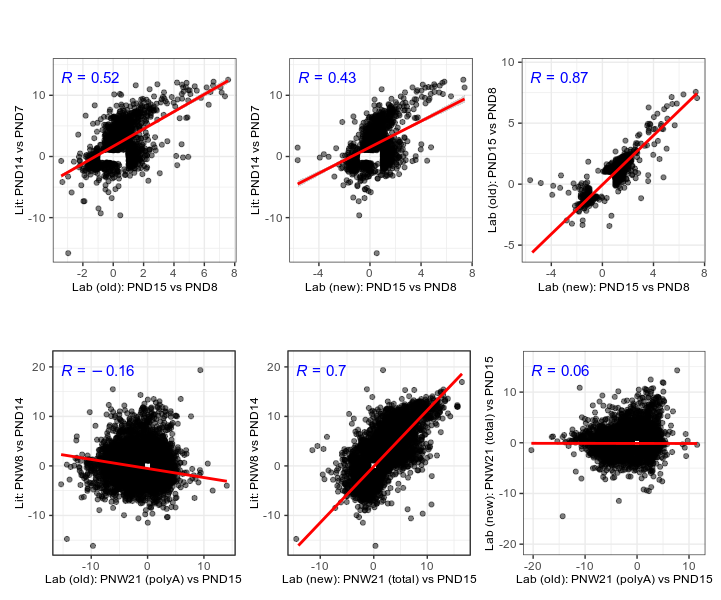
\includegraphics{thesis_files/figure-latex/dn1-1} 

}

\caption[Log\textsubscript{2} fold-change comparison of RNA-seq data
from the literature and lab (old and new)]{\textbf{Log\textsubscript{2} fold-change comparison of RNA-seq data from the literature and lab (old and new).}}\label{fig:dn1}
\end{figure}
First, we compared the gene expression of lab PND8 samples to PND7 from
literature and lab PND15 samples to PND14 from literature and discovered
a strong correlation; however, data from PNW8 and PNW21 were not well
correlated (result not shown). Following that, we performed differential
analysis on data from the lab: PND15 vs PND8 and PNW21 vs PND15, as well
as data from the literature: PND14 and PND7, and PNW8 and PND14. We
compared the log2 fold-changes from PND14 vs PND8 with PND15 vs PND8,
and PNW8 vs PND14 with PNW21 vs PND15 after differential analysis. We
discovered that the correlation between PND14 vs PND8 and PND15 vs PND8
was 52\% (R = 0.52, Pearson method) and that most of the genes were
changing in the same direction, whereas the correlation between PNW8 vs
PND14 and PNW21 vs PND15 was negative 16\% (R = -0.16; Pearson method)
and that around 50\% of the genes were changing in the opposite
direction, as shown in Figure \ref{fig:dn1}A. As a result, we incorporated the PND14
and PNW8 datasets into our project to better compare developmental
stages. We used differential analysis between PNW8 and PND14 rather than
PNW8 and PND15 because the PND14 and PND15 samples were sequenced
separately and could have unaccountable batch effects. These analyses
were then updated in the manuscript and appear in \protect\hyperlink{chapter1}{Chapter
1}.

\hypertarget{new-rna-seq-data-from-lab}{%
\subsection{New RNA-seq data from lab}\label{new-rna-seq-data-from-lab}}

Because of these limitations, we decided to generate new SCs data in the
lab. Previously, the ``Takara total RNA pico input mammalian kit v2'' was
used to generate libraries, but this kit is no longer available. The new
RNA-seq dataset was obtained from the total RNA libraries prepared using
the ``Takara total RNA pico input mammalian kit v3.'' Furthermore, PND8
and PND15 libraries were previously sequenced on the Illumina HiSeq 4000
platform, which is no longer available for sequencing at the Functional
Genomics Center Zurich (FGCZ). To avoid any technical/ batch effects, we
therefore re-sequenced the total RNA libraries from PND8 and PND15 on
the Illumina NovaSeq platform using the ``Takara total RNA pico input
mammalian kit v3'' along with the PNW21 total RNA libraries.

First, we compared the newly sequenced data to data generated previously
in the lab and from the literature. We discovered that gene expression
from newly generated PND8 data was highly correlated with data generated
in the lab previously and data from the literature. The data from the
PNW21 stage is also well correlated with the literature (result not
shown).



\begin{figure}[htbp]

{\centering 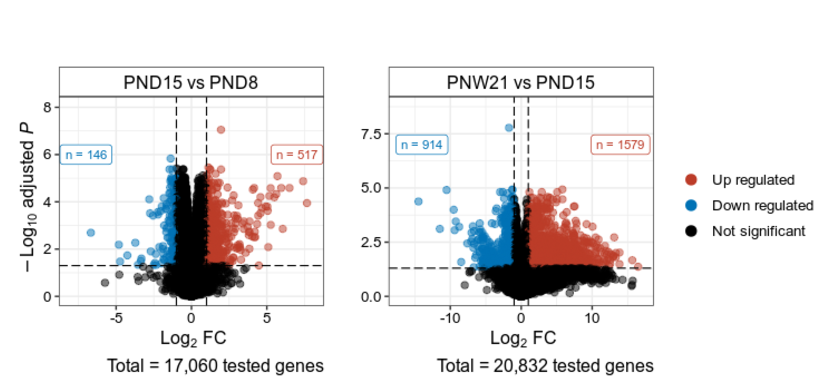
\includegraphics{thesis_files/figure-latex/dn2-1} 

}

\caption[Volcano plot of differentially expressed genes]{\textbf{Volcano plot of differentially expressed genes (adjusted \textit{P} $\leq$ 0.05 and absolute Log\textsubscript{2}FC $\geq$ 1)}.\newline
\textbf{A:} PND15 and PND8. \newline \textbf{B:} PNW21 and PND15.}\label{fig:dn2}
\end{figure}
We processed the RNA-seq data using the methods described in \protect\hyperlink{chapter1}{Chapter
1}
and \protect\hyperlink{methods}{Methods}. Following that, we conducted a differential analysis
between PND15 and PND8, as well as PNW21 and PND15. Figure \ref{fig:dn2} shows that
we found 663 genes that were differentially expressed between PND15 and
PND8, and 2,493 genes that were differentially expressed between PNW21
and PND15.

We compared log2 fold-changes from new data PND15 vs PND8 to literature
data PND14 vs PND8, and new data PNW21 vs PND15 to literature data PNW8
vs PND14. We discovered that the correlation between PND14 vs PND8 and
PND15 vs PND8 was 43\% (R = 0.43, Pearson method) and that most of the
genes were changing in the same direction, and that the correlation
between PNW8 vs PND14 and PNW21 vs PND15 was 70\% (R = 0.7; Pearson
method) and that most of the genes were changing in the same direction,
as shown in Figure \ref{fig:dn1}C, \ref{fig:dn1}D. Furthermore, we compared the lab's old data
with the new data and discovered an 87\% correlation (R = 0.87; Pearson
method) and nearly all the genes changing in the same direction for
PND15 vs PND8, whereas the correlation for PNW21 vs PND15 was 6\% (R =
0.06; Pearson method) and nearly 50\% genes changing in the opposite
direction, Figure \ref{fig:dn1}E, \ref{fig:dn1}F. This is due to the fact that the previous
PNW21 data were obtained from ployA libraries, whereas the new PNW21
data were obtained from total RNA libraries.

\hypertarget{identification-of-clusters-of-genes-with-distinct-expression-profiles}{%
\subsubsection{Identification of clusters of genes with distinct expression profiles}\label{identification-of-clusters-of-genes-with-distinct-expression-profiles}}

We discovered five clusters of genes that were differentially expressed.
We have used the union of differentially expressed genes between PND15
and PND8, as well as PNW21 and PND15, and ran k-means clustering (k = 2
to 10) on the log2 fold-changes of normalized expression values, using
PND8 samples as the baseline. Based on visual inspection, we select 7
clusters (k = 7) and merge the clusters with visually observed similar
expression profiles to obtain 5 clusters, Figure \ref{fig:dn3}.







\begin{figure}[htbp]

{\centering 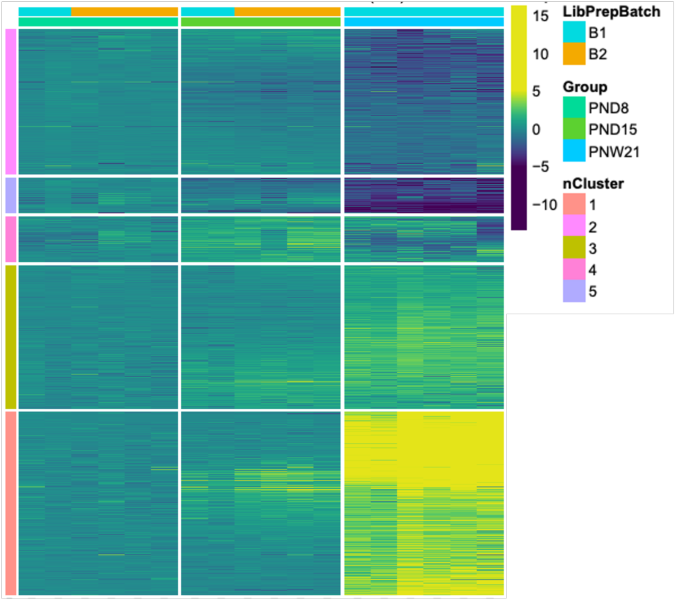
\includegraphics{thesis_files/figure-latex/dn3-1} 

}

\caption[K-means clustering of differentiallly expressed genes]{\textbf{K-means clustering (k = 5) of genes with differential expression in postnatal versus adult spermatogonial cells.}
Each row depicts a gene and each column depicts a sample. Gene
expression fold-change is calculated by subtracting mean
log\textsubscript{2} counts per million (CPM) of PND8 from PND15 and
PNW21. Samples are clustered using Ward's method and genes are ordered
by the ``MDS\_angle method'' using \texttt{seriation} (R package).}\label{fig:dn3}
\end{figure}
\hypertarget{multi-omics-data-integration-1}{%
\subsubsection{Multi-omics data integration}\label{multi-omics-data-integration-1}}

After combining data from ATAC-seq, RNA-seq, and ChIP-seq, we were able
to generate clusters of distinct genome activity. We combined these
datasets, with ATAC-seq as the starting point, \protect\hyperlink{methods}{Methods}. We classified
the differentially accessible regions (DARs) based on ATAC-seq and
RNA-seq data into distal (\textgreater{} 2.5 kb of the transcription start site,
TSS) and proximal (2.5kb of TSS). Following that, distal DARs were
divided into two groups based on increased or decreased accessibility in
PNW21, Figure \ref{fig:dn4},\ref{fig:dn6}, while proximal DARs were divided into six groups
based on increased or decreased accessibility in PNW21 and up or
down-regulation of nearby gene expression in PNW21 Figure \ref{fig:dn5}, \ref{fig:dn7}.
Category 1: increased chromatin accessibility and upregulation of
neighbouring genes; Category 2: increased chromatin accessibility and
downregulation of neighbouring genes Category 3: decreased chromatin
accessibility and downregulation of neighbouring genes, Category 4:
decreased chromatin accessibility and upregulation of neighbouring
genes, Category 5: increased chromatin accessibility with no detectable
gene expression, and Category 6: decreased chromatin accessibility with
no detectable gene expression. All such clusters had also been
identified in the previous analysis (see \protect\hyperlink{chapter1}{Chapter
1} and
(\protect\hyperlink{ref-lazarcontes_2020}{Lazar-Contes et al., 2020}), however one of the original categories (Category 5
from Figure \ref{fig:dn5}) disappeared in the new analysis. This category is related
to TSS-proximal DARs which, against expectations, increase in expression
despite a decrease in accessibility. Since expression implies promoter
accessibility, it is safe to assume that this category was attributable
to lack of comparability of the two RNAseq protocols.

To conclude, the results obtained from the newly generated RNA-seq data
from the lab are quite similar to the results generated previously We
have obtained similar results in terms of differential analysis and
multi-omics data integrations. However, a number of analyses are still
to be performed, for instance, gene-ontology analysis on differentially
expressed genes, identified clusters of gene expression, and clusters
obtained from multi-omics data integration; transcription factor motif
analysis of clusters obtained from multi-omics data integration; and
revision of figures and manuscript.

Figures \ref{fig:dn4}, \ref{fig:dn5}, \ref{fig:dn6}, \ref{fig:dn7} are enriched heatmaps that show different clusters for
distal and proximal regions. Each row represents a peak region, which is
ordered by the ATAC signal. The mid-x-axis corresponds to the centre of
a peak region and is extended to +/1 kbp. The ATAC heatmap's colour key
represents the signal. For RNA-seq, the fold-change in gene expression
is calculated by subtracting the mean log\textsubscript{2} CPM of PND8
from all samples.


\begin{figure}[htbp]

{\centering 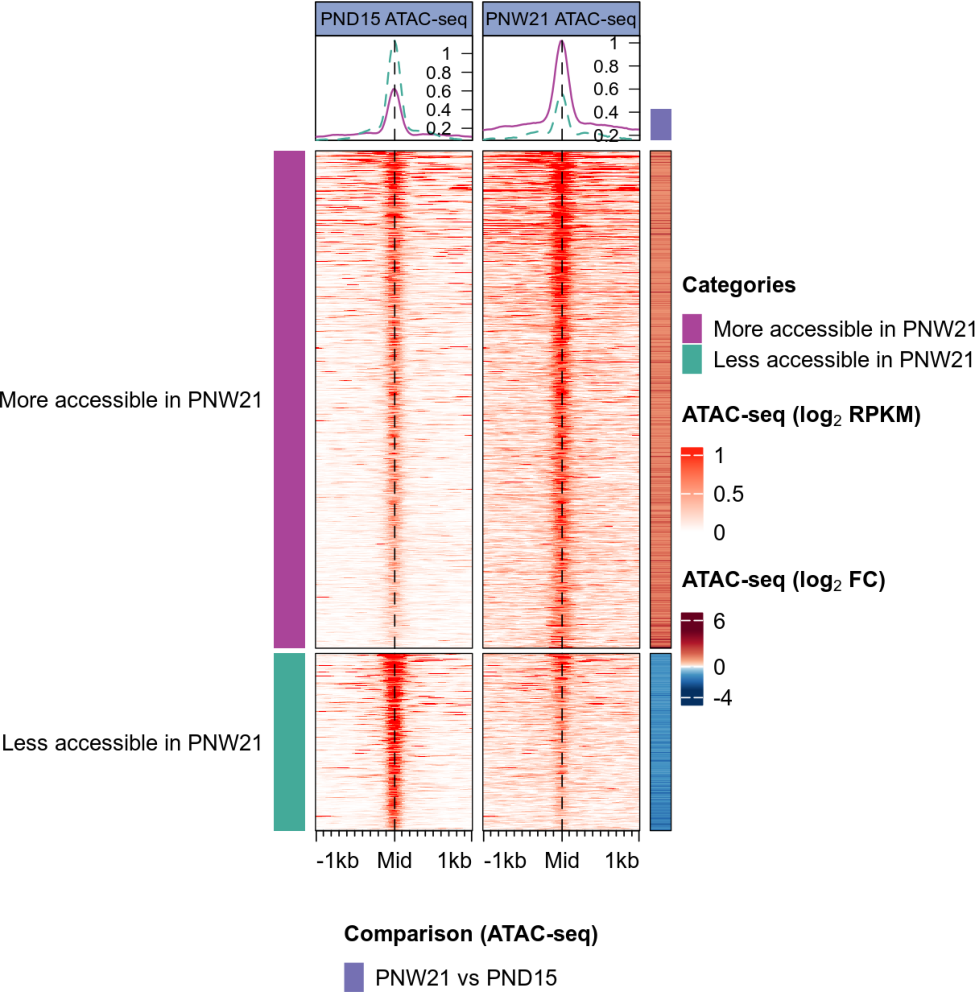
\includegraphics{thesis_files/figure-latex/dn4-1} 

}

\caption[Enriched heatmap of distal DARs]{\textbf{Enriched heatmap of distal differentially accessible regions.}}\label{fig:dn4}
\end{figure}

\begin{figure}[htbp]

{\centering 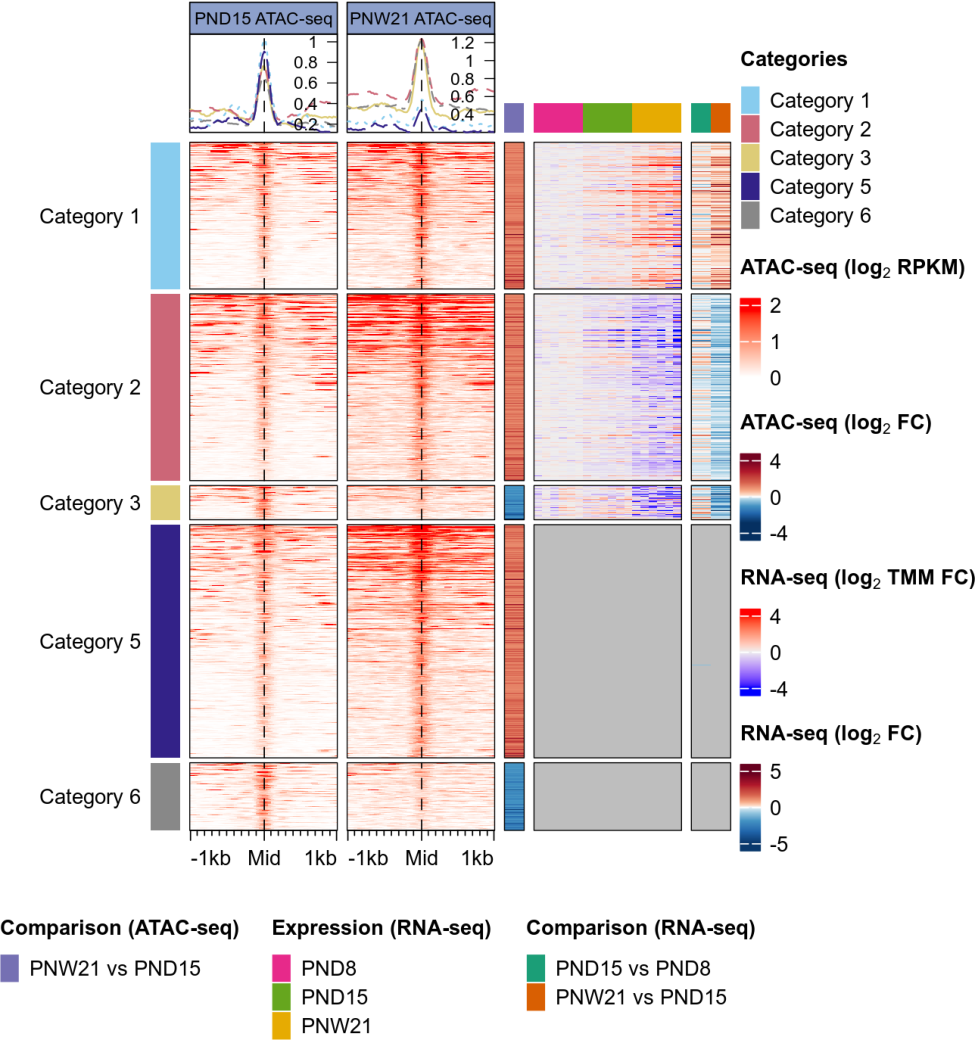
\includegraphics{thesis_files/figure-latex/dn5-1} 

}

\caption[Enriched heatmap of proximal DARs]{\textbf{Enriched heatmap of proximal differentially accessible regions.}}\label{fig:dn5}
\end{figure}

\begin{figure}[htbp]

{\centering 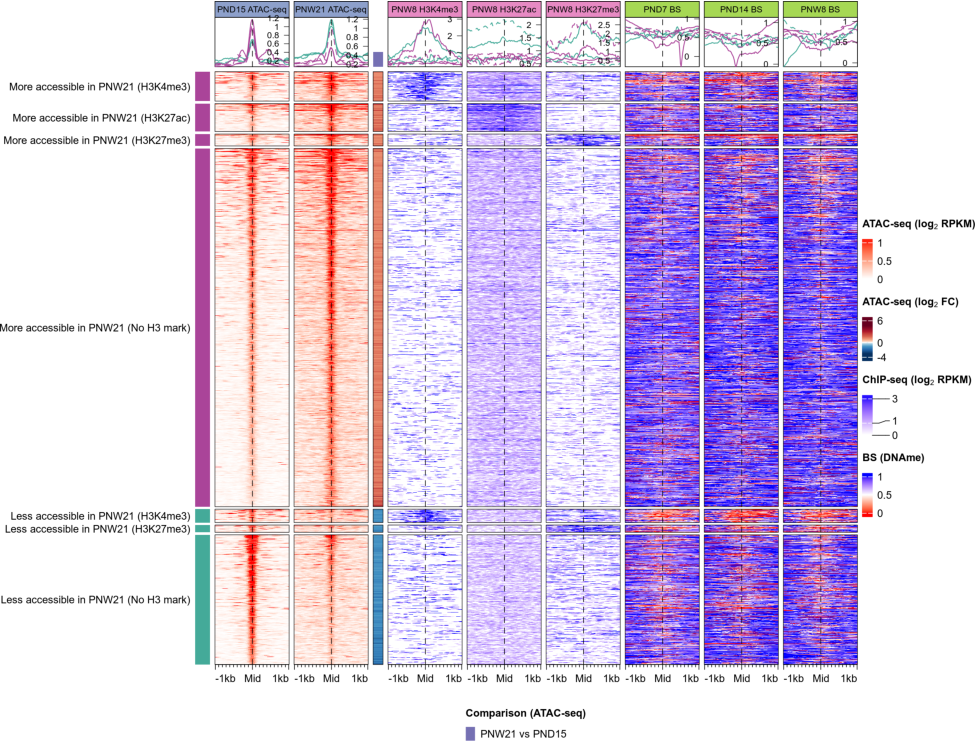
\includegraphics{thesis_files/figure-latex/dn6-1} 

}

\caption[Enriched heatmap of distal DARs with ChIP-seq and BS-seq data]{\textbf{Enriched heatmap of distal differentially accessible regions with ChIP-seq and BS-seq data.}}\label{fig:dn6}
\end{figure}

\begin{figure}[htbp]

{\centering 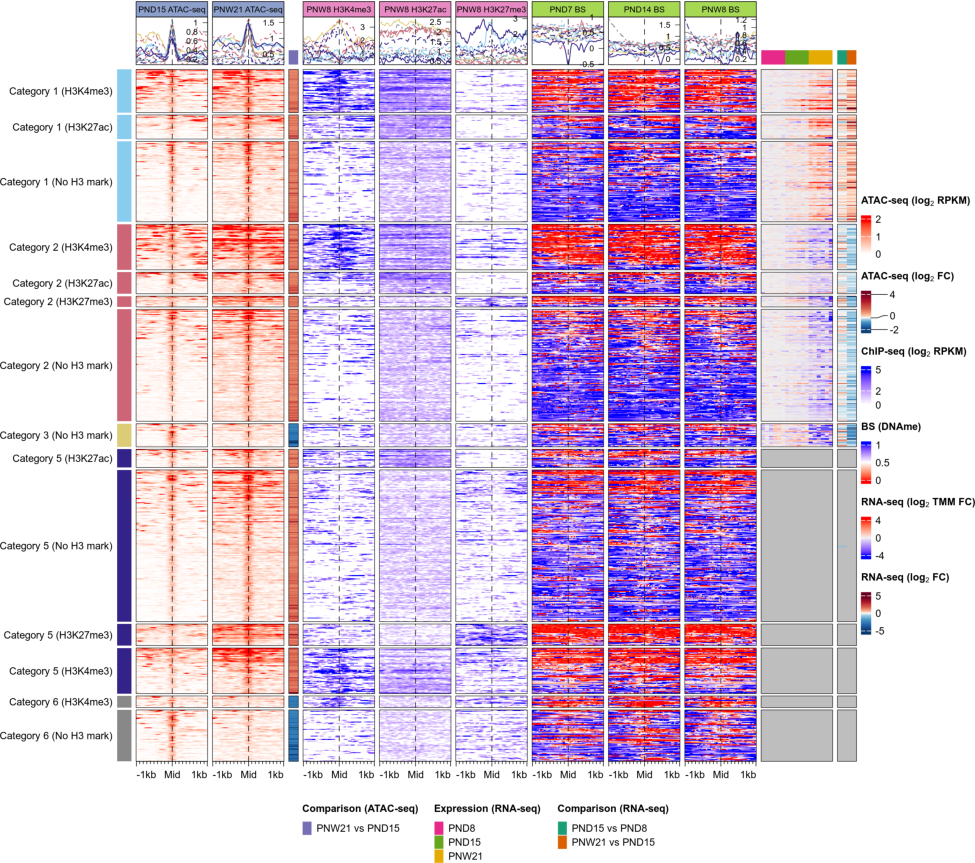
\includegraphics{thesis_files/figure-latex/dn7-1} 

}

\caption[Enriched heatmap of proximal DARs with ChIP-seq and BS-seq data]{\textbf{Enriched heatmap of proximal differentially accessible regions with ChIP-seq and BS-seq data.}}\label{fig:dn7}
\end{figure}
\hypertarget{graphical-abstract}{%
\section{Graphical Abstract}\label{graphical-abstract}}
\begin{figure}[htbp]

{\centering 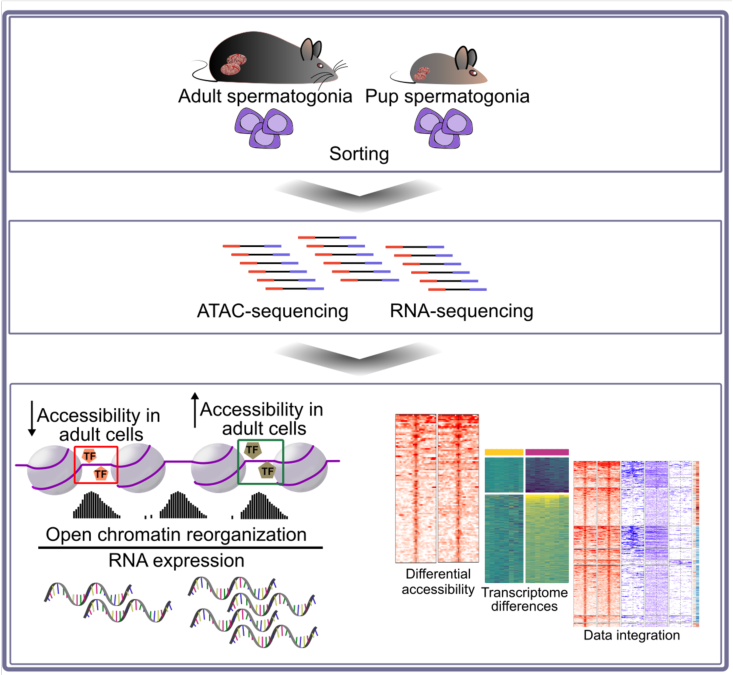
\includegraphics{thesis_files/figure-latex/dga-1} 

}

\caption[Graphical abstract]{Graphical abstract.}\label{fig:dga}
\end{figure}
\newpage

\hypertarget{abstract}{%
\section{Abstract}\label{abstract}}

Stem cells have the capacity to self-renew and differentiate to give
rise to tissues. In mammals, spermatogonial stem cells are unique
undifferentiated cells in the male germline that are present throughout
life and produce functional sperm. They have a remarkable dynamic
transcriptome between postnatal life and adulthood, thought to allow
adaptation to the maturing gonadal environment. To assess if chromatin
remodelling is associated with this dynamic, we characterized chromatin
accessibility in postnatal and adult spermatogonial cells in mice using
ATAC-seq. Extensive changes in chromatin accessibility were observed in
spermatogonial cells across postnatal development, that correlate with
distinct gene expression profiles and transcription factor motif
enrichment. We identify genomic regions with differential chromatin
accessibility in adult spermatogonial cells, that are marked by distinct
histone modifications and are situated in proximity to the transcription
start site of genes important for cell maintenance and proliferation.
Some of these regions correspond to transposable element subtypes
enriched in multiple transcription factor motifs and with increased
transcription. Together, our results reveal profiles of chromatin
organization, histone modifications and gene expression in
spermatogonial cells, and underscore the dynamic nature of the germline
genome.

\newpage

\hypertarget{introduction}{%
\section{Introduction}\label{introduction}}

Spermatogonial cells are cells in male gonads that actively self-renew
and differentiate into spermatogenic cells to produce adult gametes. In
mice, they become active one to two days after birth, when they exit
mitotic arrest and start dividing, to populate the basement membrane of
seminiferous tubules. During the first week of postnatal life, a
population of spermatogonial cells continues to proliferate and gives
rise to undifferentiated Asingle (As), Apaired (Apr) and Aaligned (Aal)
cells. The remaining spermatogonia differentiate to form chains of
daughter cells that become primary and secondary spermatocytes around
postnatal day (PND) 10 to 12. Spermatocytes undergo meiosis and give
rise to haploid spermatids that develop into spermatozoa. Spermatozoa
are then released in the lumen of the seminiferous tubules and continue
to mature in the epididymis until becoming capable of fertilization by
PND 42-48 (\protect\hyperlink{ref-kubota2018}{Kubota \& Brinster, 2018}; \protect\hyperlink{ref-thebiol2017}{Oatley \& Griswold, 2017}; \protect\hyperlink{ref-rooij2017}{Rooij, 2017}).

Recent work using population or single-cell RNA sequencing (RNA-seq)
showed that distinct transcriptional profiles characterize
spermatogonial cells in postnatal and adult life (\protect\hyperlink{ref-green2018}{C. D. Green et al., 2018}; \protect\hyperlink{ref-hammoud2014}{Hammoud et al., 2014}, \protect\hyperlink{ref-hammoud2015}{2015}; \protect\hyperlink{ref-hermann2018}{Hermann et al., 2018}; \protect\hyperlink{ref-law2019}{N. C. Law, Oatley, \& Oatley, 2019}). During the first week
after birth, spermatogonia have unique features necessary for their
rapid establishment and expansion along the basement membrane. This
includes high expression of genes involved in cell cycle regulation,
stem cell proliferation, transcription and RNA (\protect\hyperlink{ref-grive2019}{Grive et al., 2019}). In
comparison, in the adult testis, genes are involved in the maintenance
of a steady spermatogonial cells population, with a balance between
proliferation and differentiation to ensure sperm formation
predominates. This includes pathways related to paracrine signalling and
niche communication, as well as mitochondrial function and oxidative
phosphorylation (\protect\hyperlink{ref-grive2019}{Grive et al., 2019}; \protect\hyperlink{ref-hermann2018}{Hermann et al., 2018}). Epigenetic changes such as
histone tail posttranslational modifications and DNA methylation
accompany transcriptional differences in spermatogonial cells across
postnatal stages (\protect\hyperlink{ref-hammoud2014}{Hammoud et al., 2014}, \protect\hyperlink{ref-hammoud2015}{2015}). However, little is known
about the accessible chromatin landscape, during the transition from
postnatal to the adult stage.

We examined chromatin reorganization in the transition from postnatal to
adult spermatogonia and its functional relevance by profiling chromatin
accessibility by ATAC-seq (assay for transposase-accessible chromatin
with high-throughput sequencing) using an Omni-ATAC protocol
(\protect\hyperlink{ref-corces2017}{Corces et al., 2017}) and integrating data with transcriptomic and epigenetic
profiles. The results show that chromatin is extensively remodelled in
spermatogonial cells during development, and its accessibility is
increased at several genomic regions particularly transposable elements
(TEs), that correlate with transcriptional and epigenetic signatures.

\hypertarget{results}{%
\section{Results}\label{results}}

\hypertarget{enrichment-of-spermatogonial-cells-from-postnatal-and-adult-mouse-testis}{%
\subsection{Enrichment of spermatogonial cells from postnatal and adult mouse testis}\label{enrichment-of-spermatogonial-cells-from-postnatal-and-adult-mouse-testis}}

We collected testes from mouse pups at postnatal days (PND) 8 and 15 and
from males at postnatal week (PNW) 20, and prepared cell suspensions by
enzymatic digestion. Spermatogonial cells were enriched by
fluorescence-activated cell sorting (FACS) using surface markers (Supp. Figure \ref{fig:ds1a}A) (\protect\hyperlink{ref-kubota2004a}{Kubota, Avarbock, \& Brinster, 2004a}). Immunocytochemistry using PLZF, a well-established
marker of undifferentiated spermatogonia (\protect\hyperlink{ref-costoya2004}{Costoya et al., 2004}), confirmed that
our preparation was enriched in spermatogonial cells, with 85-95\% PLZF+
cells after FACS compared to 3-6\% PLZF+ cells before (Supp. Figure \ref{fig:ds1a}B).
Transcriptomic analyses by RNA-seq validated the spermatogonial identity
of the cells, showing high expression of stem cell and undifferentiated
spermatogonial markers, and low expression of somatic cells (Leydig and
Sertoli cells) markers both at PND 8 and 15 (Supp. Figure \ref{fig:ds1b}C).

\hypertarget{chromatin-is-remodelled-in-spermatogonial-cells-during-the-development}{%
\subsection{Chromatin is remodelled in spermatogonial cells during the development}\label{chromatin-is-remodelled-in-spermatogonial-cells-during-the-development}}

We profiled chromatin accessibility in postnatal and adult
spermatogonial cells using an Omni-ATAC protocol (\protect\hyperlink{ref-corces2017}{Corces et al., 2017}).
Omni-ATAC has a higher signal-to-noise ratio than classical ATAC-seq and
can be used with low input material (a few hundred cells). Accessible
regions in the genome were identified by peak-calling on merged
nucleosome-free fragments (NFF). Following the removal of lowly enriched
regions, 158,978 regions were selected for downstream analyses (see
Methods section for details). Most Tn5-accessible regions are intergenic
(38\%) and located in gene bodies (33\%) or in the proximity of a
transcription start site (TSS) (28\% +/-1 kb from TSS) (Supp. Figure \ref{fig:ds2a}A). 3212
differentially accessible regions were identified between PND15 and
adult spermatogonia with the majority showing a gain in accessibility in
adult cells (Figure \ref{fig:df1a}A and \protect\hyperlink{st}{Table S1}). Regions of differential
accessibility are predominantly intergenic (45\%) and intronic (34\%), and
15\% of all differentially accessible regions are +/- 1kb from a TSS
(Figure \ref{fig:df1a}B). Gene ontology (GO) analysis, showed that regions with
increased accessibility in adult spermatogonia are associated with cell
fate and stem cell population maintenance, protein metabolism and RNA
metabolic processes (Figure \ref{fig:df1b}C and \protect\hyperlink{st}{Table S1}). Separate GO analyses
depending on genomic location showed that regions located in gene bodies
(mainly introns) are enriched for terms related to reproduction and
protein metabolism, whilst regions close to or overlapping with a TSS
relate to cell fate specification and tissue morphogenesis (Supp. Figure \ref{fig:ds2b}B and
\protect\hyperlink{st}{Table S1}). Regions with decreased accessibility in adult spermatogonia
are predominantly located in intergenic regions and associated with
multiple terms related to embryonic development (Figure \ref{fig:df1b}C and \protect\hyperlink{st}{Table S1}).

\hypertarget{differentially-accessible-chromatin-regions-associated-with-distinct-gene-expression-dynamics}{%
\subsection{Differentially accessible chromatin regions associated with distinct gene expression dynamics}\label{differentially-accessible-chromatin-regions-associated-with-distinct-gene-expression-dynamics}}

To assess the relevance of changes in chromatin accessibility, we first
integrated our ATAC-Seq data with transcriptomic datasets and examined
the correlation between chromatin states and transcriptome. We conducted
RNA-seq analyses on postnatal spermatogonial cells and used published
data from Thy1+ adult spermatogonial cells. We found that 719 genes are
differentially expressed in spermatogonial cells between PND8 and PND15,
with 515 being upregulated and 212 downregulated (Figure \ref{fig:df2a}A and \protect\hyperlink{st}{Table S2}).
Fast Gene Set Enrichment Analysis (FGSEA) showed that pathways related
to RNA processing and splicing, cell cycle, redox homeostasis and
protein catabolism are downregulated between PND8 and PND15 while
pathways associated with cellular transport, exocytosis and signal
transduction are upregulated (Figure \ref{fig:df2a}B and \protect\hyperlink{st}{Table S2}). Comparable analyses
using published RNA-seq data from PND14 and adult spermatogonia cells
(\protect\hyperlink{ref-hammoud2014}{Hammoud et al., 2014}, \protect\hyperlink{ref-hammoud2015}{2015}) similarly identified transcriptional
changes between postnatal and adult stages (Fig. S?A and \protect\hyperlink{st}{Table S2}) and
downregulation of pathways related to RNA processing, ribosome
biogenesis and cell cycle in adults compared to postnatal cells.
Pathways related to developmental programs and mitochondrial functions
were also downregulated and those related to spermatogenesis or
involving cytokine signalling were upregulated (Fig. S? and \protect\hyperlink{st}{Table S2}).

To integrate chromatin accessibility and transcriptomic datasets, we
first divided differentially-accessible regions into proximal (situated
less than +/- 2.5 kb from a TSS) and distal (situated more than +/- 2.5
kb from a TSS) following ENCODE practice (\protect\hyperlink{ref-ausers2011}{Becker, 2011}; \protect\hyperlink{ref-harrow2012}{Harrow et al., 2012}; \protect\hyperlink{ref-thurman2012}{Thurman et al., 2012}). For proximal regions, we further defined 6 different
categories based on the change in expression of the nearest gene. The
first two include proximal regions with increased chromatin
accessibility and upregulated (Category 1) or downregulated (Category 2)
expression of the nearest gene. Category 3 and 4 include regions of less
chromatin accessibility with the nearest gene either downregulated or
upregulated, respectively. Category 5 and 6 include regions with
increased or decreased chromatin accessibility respectively, whose
nearest gene is not expressed in spermatogonial cells (Figure \ref{fig:df3a}A and \protect\hyperlink{st}{Table S3})).

\hypertarget{differentially-accessible-chromatin-regions-associated-with-distinct-epigenetic-profiles}{%
\subsection{Differentially accessible chromatin regions associated with distinct epigenetic profiles}\label{differentially-accessible-chromatin-regions-associated-with-distinct-epigenetic-profiles}}

Next, we examined the relationship between chromatin accessibility and
epigenetic marks using published ChIP-seq and bisulfite sequencing (BS)
datasets from Thy1+ spermatogonia (\protect\hyperlink{ref-hammoud2014}{Hammoud et al., 2014}, \protect\hyperlink{ref-hammoud2015}{2015}). Profiles
of histone marks including H3K4me3, H3K27ac and H3K27me3 in adult
spermatogonial cells, and DNA methylation in PND7, PND14 and adult
spermatogonial cells were used. \ldots..analyses showed that for a subset
of regions in Category 1, there is an overlap with active H3K4me3,
H3K27ac or dual H3K4me3/K27ac modifications, and an overall lack of
H3K27me3 (Figure \ref{fig:df3a}B and \protect\hyperlink{st}{Table S3}). Notably, several of the genes in
Category 1 with chromatin opening marked by histone modification(s) are
known regulators of stem cell potency. Pdpk1 promoter region was marked
by dual H3K4me3/K27ac, while Pdpk1 mRNA was upregulated in adult
spermatogonia (Supp. Figure \ref{fig:ds3}A). Pdpk1 (phosphoinositide-dependent protein
kinase 1) is a glycolysis factor important for stem cell self-renewal
(\protect\hyperlink{ref-chen2020}{W. Chen et al., 2020}; \protect\hyperlink{ref-kanatsu-shinohara2016}{Kanatsu-Shinohara et al., 2016}). In contrast, the Gata2 promoter
region was marked by the bivalent H3K4me3/K27me3 mark, while Gata2
expression showed an upregulation across testis maturation (Supp. Figure \ref{fig:ds3}).
Gata2 (GATA-binding factor 2) is a known target of NANOS2, an essential
regulator of spermatogonial stem cell potential (\protect\hyperlink{ref-barrios2010}{Barrios et al., 2010}; \protect\hyperlink{ref-sada2009}{Sada, Suzuki, Suzuki, \& Saga, 2009}). Other exemplary genes in Category 1 include pyruvate
cellular carriers Slc25a18, Slc23a1 and Slc2a5, suggesting differences
in glycolysis regulation in adult spermatogonial cells (\protect\hyperlink{st}{Table S3}).
Notably, we found increased chromatin accessibility at the TSS of GDNF
receptor Gfra2 (Figure \ref{fig:df3b}C). At the mRNA level, Gfra2displayed a marked
upregulation in adult spermatogonial cells, indicating an increased
utilization of GFRA2 receptors in adult spermatogonial cells compared to
early postnatal stages, in which GFRA1-mediated signalling is dominant
(Figure \ref{fig:df3b}C) (\protect\hyperlink{ref-grive2019}{Grive et al., 2019}; \protect\hyperlink{ref-hammoud2015}{Hammoud et al., 2015}). We also observed increased
chromatin accessibility and upregulation of DNA damage responsive gene
Fus, and the multifunctional redox gene Prdx4 (\protect\hyperlink{st}{Table S3}).

Interestingly, the highest number of differentially accessible chromatin
regions were in Category 2, and included proximal regions with increased
chromatin accessibility and decreased expression of nearby genes in
adult spermatogonia, indicative of active repression taking place (Fig.
3A and \protect\hyperlink{st}{Table S3}). A subset of Category 2 regions was marked by H3K27me3
together with H3K4me3 and mainly associated with developmental genes
such as Satb1 and Hmx1, (Supp. Figure \ref{fig:ds3}B). Other developmental genes such as
Tbx4 also displayed a decreased accessibility and an increase in mRNA
expression (Figure \ref{fig:df3b}C). GO enrichment analysis revealed that regions in
Category 2 are associated with regulation of cell cycle, RNA processing,
DNA repair and cell division (\protect\hyperlink{st}{Table S4}). Such an example is is Fgf8,
important for Fgf8-Fgfr1 mediated maintenance of undifferentiated
spermatogonia (\protect\hyperlink{ref-hasegawa2014}{Hasegawa \& Saga, 2014}). Fgf8 showed increased chromatin
accessibility close to its TSS and a downregulated expression in adult
spermatogonia, in agreement with recent findings from scRNA-seq data
suggesting downregulation of Fgfr1-mediated signalling with age(Fig.
S3B) (\protect\hyperlink{ref-grive2019}{Grive et al., 2019}; \protect\hyperlink{ref-hasegawa2014}{Hasegawa \& Saga, 2014}).

Regions in Category 3 displayed decreased chromatin accessibility and
downregulation of nearby genes in adult spermatogonia and were mostly
depleted of any of the 3 histone marks investigated (Figure \ref{fig:df3a}A and \ref{fig:df3a}B). GO
enrichment on the nearby genes revealed an association with
developmental processes and WNT signalling (\protect\hyperlink{st}{Table S4}). A notable example
we identified in this category is Pdgfra, a gene involved in the hepatic
stellate cell activation pathway, which was recently identified by
scRNA-seq to be upregulated in spermatogonial stem cells in the immature
testis compared to the adult stage (\protect\hyperlink{ref-hermann2018}{Hermann et al., 2018}). Pdgfra displayed a
marked downregulation in adult spermatogonia, and a decrease in
chromatin accessibility overlapping its TSS (Figure \ref{fig:df3b}C). Another example
of a gene important for early postnatal spermatogonial cell
establishment is Dap2ip, which we also found to carry a marked decrease
in chromatin accessibility at its TSS and lower expression in adult
spermatogonial cells (Supp. Figure \ref{fig:ds3}C). Surprisingly, we also identified a
category of proximal regions (Category 4) with decreased accessibility
(\textless20 regions) at genes that were upregulated in adult spermatogonial
cells and with a previously uncharacterized role in spermatogonial cells
(Figure \ref{fig:df3a}A). Notably, DNAme profiles across postnatal stages did not show
any significant change across any of the 6 categories of proximal
regions, suggesting a relatively stable DNAme profile in the transition
from early postnatal to adult stage (Supp. Figure \ref{fig:ds3}D). Aside from proximal
regions, we also identified numerous distal regions with differential
chromatin accessibility between PND15 and adult spermatogonial cells
(Supp. Figure \ref{fig:ds4}A). Similar to proximal regions, accessibility in distal regions
mainly increased in adult spermatogonial cells compared to the early
postnatal stage. When integrating the literature ChIP-seq data, we
observed enrichment for H3K4me3, H3K27ac and H3K27me3 at a small number
of the differentially accessible distal regions, indicative of potential
regulatory roles (Supp. Figure \ref{fig:ds4}B and \protect\hyperlink{st}{Table S3}). Similar to proximal regions,
DNAme levels did not display major changes in the transition from early
postnatal to adult stage (Supp. Figure \ref{fig:ds4}B). Taken together, our data
integration reveals novel associations between chromatin regions of
differential accessibility, histone marks and gene transcription in
spermatogonial cells from postnatal to adult stages of development. They
suggest that chromatin accessibility is a mechanism of control of
transcriptional programs and of certain signalling pathways during
development.

\hypertarget{accessibility-changes-at-open-chromatin-regions-carry-binding-sites-for-distinct-families-of-transcription-factors}{%
\subsection{Accessibility changes at open chromatin regions carry binding sites for distinct families of transcription factors}\label{accessibility-changes-at-open-chromatin-regions-carry-binding-sites-for-distinct-families-of-transcription-factors}}

Transcription factors (TFs) are essential for establishing and
maintaining transcriptional programs across developmental stages in
cells Fushan et al. (\protect\hyperlink{ref-fushan2015}{2015}). To examine if regions of different
chromatin accessibility between PND15 and adult spermatogonia are
enriched in regulatory elements such as TF binding motifs, we performed
motif enrichment analysis using the Hypergeometric Optimization of Motif
EnRichment (HOMER) tool (\protect\hyperlink{ref-heinz2010}{Heinz et al., 2010}). In regions with increased
chromatin accessibility, we identified 41 enriched TF motifs (q-value
\(\leq\) 0.05) (Figure \ref{fig:df4a}A). Top candidates by significance (q-value \(\leq\)
0.0001) are members of the Fos/Jun family (FOS, FOSB, FOSL1 and FOSL2,
JUN, JUNB and JUND) (Figure \ref{fig:df4a}B). Notably, at the mRNA level, some of the
TFs displayed age-specific differences (log\textsubscript{2}CPM \(\geq\) 1 and abs log\textsubscript{2}
fold change \(\geq\) 1): Fos,Junb and Jund were downregulated in adult
spermatogonial cells (Figure \ref{fig:df4b}C). JUN, FOS and CREB are all part of the
AP-1 (activating protein-1) superfamily, and play an important role in
regulating cell proliferation and death, by mediating the
senescence-associated chromatin and transcriptional landscape
(\protect\hyperlink{ref-martuxednez-zamudio2020}{Martínez-Zamudio et al., 2020}; \protect\hyperlink{ref-shaulian2002}{Shaulian \& Karin, 2002}). JUND and c-FOS specifically
promote the proliferative potential of spermatogonial stem cells
(\protect\hyperlink{ref-he2008}{He et al., 2008}; \protect\hyperlink{ref-wang2018}{M. Wang et al., 2018}). USF1 and POU3F1, 2 factors important in the
maintenance of the spermatogonial stem cell pool also displayed enriched
binding motifs in the more accessible regions. However, their mRNA
levels were downregulated in adult spermatogonial cells (Figure \ref{fig:df4b}C)
{[}(\protect\hyperlink{ref-faisal2019}{Faisal et al., 2019}, \protect\hyperlink{ref-faisal2019}{2019}). POU3F1 is a GDNF-regulated TF, which has
been shown to play an important role in promoting spermatogonial cell
self-renewal capacity (\protect\hyperlink{ref-niu2011}{Niu et al., 2011}; \protect\hyperlink{ref-wu2010a}{Xin Wu et al., 2010}). Notably, Pou3f1
downregulation in adult spermatogonial cells coincides with marked
downregulation of Gfra1 and upregulation of Gfra2 (Figure \ref{fig:df3b}C and \protect\hyperlink{st}{Table S2}).TF motif analysis using HOMER also revealed enriched binding sites
for retinoic acid receptors such as RXRa and RARa
(Figure \ref{fig:df4a}A). Recently, expression of RA receptors Rxra and
Rara was reported in the stem cell-containing population of
spermatogonial cells in both pup and adult testis, together with
evidence that their utilization in spermatogonial cells is vastly
dependent on the niche microenvironment (\protect\hyperlink{ref-lord2018}{Lord, Oatley, \& Oatley, 2018}).

To check if some TF binding motifs are preferentially enriched in
certain genomic locations, we performed motif enrichment analysis for
more accessible chromatin regions situated in gene bodies, intergenic
regions and in regions +/- 1kb from TSS. We identified several TF motifs
specifically enriched in intergenic regions, specifically members of the
ubiquitously expressed NF-Y complex, NF-YA, NF-YB and NF-YC (Figure \ref{fig:df4b}D).
In mESCs, NF-Y TF family members located in distal regions facilitate a
permissive chromatin conformation and play an important role in the
expression of core ESC pluripotency genes (\protect\hyperlink{ref-oldfield2014}{Oldfield et al., 2014}). Furthermore,
NF-YA/B motif enrichment has also been found in regions of open
chromatin in human spermatogonial cells (\protect\hyperlink{ref-guo2017}{Guo et al., 2017}).

Although regions of more accessible chromatin encompass the majority of
the differentially accessible regions in adult spermatogonia compared to
PND15, less accessible chromatin also displayed a high number of
enriched TF binding motifs (Figure \ref{fig:df4a}A). Notably, almost all of these TF
motifs were uniquely enriched in the regions of decreased chromatin
accessibility and predominantly associated with developmental factors.
Top hits included members of the FOX family (FOXO1, FOXO3, FOXP2, FOXK1,
FOXA2) and members of the ETS and ETS-related families (ETS1, GABPA,
ETV4, ELF1, ELF3) (Figure \ref{fig:df4a}B). The gene expression levels of most of these
TFs were decreased in adult spermatogonial cells (Figure \ref{fig:df4a}A). FOXO1 is a
pivotal regulator of the self-renewal and differentiation of
spermatogonial stem cells in both pup and adult testis, via the PI3K-Akt
signalling pathway (\protect\hyperlink{ref-chan2014}{F. Chan et al., 2014}; \protect\hyperlink{ref-goertz2011}{Goertz, Wu, Gallardo, Hamra, \& Castrillon, 2011}). The roles of the various
ETS-related TFs in spermatogonial cells have not been clarified, however
recently published data found ETV4 in the stem-cell enriched fraction of
the spermatogonial population, particularly during the spermatogonial
stem cell pool establishment immediately after birth (\protect\hyperlink{ref-cheng2020}{Cheng et al., 2020}; \protect\hyperlink{ref-law2019}{N. C. Law et al., 2019}). Motif enrichment analysis on the regions with decreased
chromatin accessibility situated in the gene body and intergenic regions
revealed that TFs are important in numerous developmental processes
(FOXC1, FOXJ2, FOXM1, LHX6) were specifically enriched in intergenic
regions of decreased chromatin accessibility (Figure \ref{fig:df4b}D). This is
consistent with the association of intergenic regions with embryonic
development-related GO terms that we previously detected (Figure \ref{fig:df1b}C). Our
findings provide a detailed characterization of the enriched TF motifs
present at the regions of dynamic accessibility between PND15 and adult
spermatogonial populations and point towards novel candidate regulators
of the differential transcriptome of the pup and adult mouse
spermatogonia.

\hypertarget{chromatin-accessibility-at-transposable-elements-undergoes-significant-remodelling-in-the-transition-from-postnatal-to-adult-spermatogonia}{%
\subsection{Chromatin accessibility at transposable elements undergoes significant remodelling in the transition from postnatal to adult spermatogonia}\label{chromatin-accessibility-at-transposable-elements-undergoes-significant-remodelling-in-the-transition-from-postnatal-to-adult-spermatogonia}}

Transposable elements (TEs) are under tight control in the germline,
through coordinated epigenetic mechanisms involving DNA methylation,
chromatin silencing and PIWI proteins -- piRNA pathway (\protect\hyperlink{ref-deniz2019}{Deniz, Frost, \& Branco, 2019}; \protect\hyperlink{ref-thompson2016}{Thompson, Macfarlan, \& Lorincz, 2016}). Recent evidence suggests an important role for long
terminal repeat (LTR) - type elements, specifically for ERVKs, the
youngest class of endogenous retroviruses (ERVs), in the transcriptional
regulation of mRNAs and long non-coding RNAs (lncRNAs) during
mitosis-to-meiosis transition (\protect\hyperlink{ref-davis2017}{Davis et al., 2017}; \protect\hyperlink{ref-sakashita2020}{Sakashita et al., 2020}). Furthermore,
accessibility analysis at LTRs in mitotic and meiotic germ cells,
revealed a unique chromatin accessibility landscape in spermatogonial
cells, compared to the rest of the germ cells in the testis
(\protect\hyperlink{ref-sakashita2020}{Sakashita et al., 2020}). To explore potential differences in TEs regulation
driven by postnatal age, we compared the accessibility of TEs in PND15
and adult spermatogonia. For this purpose, we quantified the ATAC-seq
reads overlapping TEs defined by UCSC RepeatMasker and performed
differential accessibility analysis at the subtype level (see Methods
section). Our results revealed that the transition from PND15 to the
adult stage is accompanied by significant chromatin accessibility
differences at 135 TE subtypes (Figure \ref{fig:df5a}A and 5B and \protect\hyperlink{st}{Table S5}). Although
most of the differentially accessible TE subtypes displayed a decrease
in chromatin accessibility between PND15 and adult stages (68,9\%,
93/135) (Figure \ref{fig:df5a}A), we also observed 42 TE subtypes which increased in
accessibility in adult spermatogonia (Figure \ref{fig:df5a}B). Of note, more accessible
subtypes also displayed an increased expression in adult spermatogonia
compared to the early postnatal stage (Figure \ref{fig:df5a}B). TE loci within the
subtypes harbouring changes in chromatin accessibility were situated in
intergenic and intronic regions (68\% intergenic and 25\% intronic), and
around 6\% were located in the proximity of a gene (+/- 1kb from a TSS)
(Figure \ref{fig:df5a}C). LTRs were the most abundant TEs to display changes in
chromatin accessibility, specifically ERVK and ERV1 subtypes (Figure \ref{fig:df5a}A
and 5B). Exemplary ERVK subtypes harbouring less accessible chromatin
included RLTR17, RLTR9A3, RLTR12B and RMER17B (\protect\hyperlink{st}{Table S5}). Enrichment of
RLTR17 and RLTR9 repeats have been reported previously in mESCs,
specifically at TFs important for pluripotency maintenance such as Oct4
and Nanog (\protect\hyperlink{ref-fort2014}{Fort et al., 2014}). Interestingly, we identified the promoter region
of the lncRNA Lncenc1, an important regulator of pluripotency in mESCs
(\protect\hyperlink{ref-fort2014}{Fort et al., 2014}; \protect\hyperlink{ref-sun2018}{Sun et al., 2018}), harboring several LTR loci with decreased
accessibility in our adult spermatogonia, with the RLTR17 locus falling
within the TSS of Lncenc1. This decrease in accessibility correlated
with a marked decrease in expression of Lncenc1 in adult spermatogonia
(Figure \ref{fig:df5a}D). Lncenc1 (also known as Platr18) is part of the
pluripotency-associated transcript (Platr) family of lncRNAs which were
recently identified as potential regulators of the
pluripotency-associated genes Oct4, Nanog and Zfp42 in mESCs (\protect\hyperlink{ref-bergmann2015}{Bergmann et al., 2015}; \protect\hyperlink{ref-dann2008}{Dann et al., 2008}; \protect\hyperlink{ref-wu2018}{D. C. Wu et al., 2018}). We were also able to identify several other
Platr genes, such as Platr27 and Platr14, for which the TSS overlapped
LTRs with reduced accessibility, RLTR17 and RLTR16B\_MM, respectively
(Figure \ref{fig:df5a}D and \protect\hyperlink{st}{Table S5}). These 2 pluripotency-associated transcripts also
showed a decrease in mRNA expression in adult spermatogonia, while their
expression was unchanged between PND8 and PND15 (Figure \ref{fig:df5a}D and \protect\hyperlink{st}{Table S5}).
The remaining LTR subtypes with decreased accessibility in adult
spermatogonia belonged to the ERV1, ERVL and MaLR families (Figure \ref{fig:df5a}A).
Only very few other non-LTR TEs showed a decrease in chromatin
accessibility, with 7 DNA element subtypes, 2 Satellite subtypes and 1
LINE subtype, respectively (Figure \ref{fig:df5a}A and \protect\hyperlink{st}{Table S5}). Emerging evidence
suggests an important contribution of TEs in providing tissue-specific
substrates for TF binding (\protect\hyperlink{ref-fort2014}{Fort et al., 2014}; \protect\hyperlink{ref-sundaram2014}{Sundaram et al., 2014}; \protect\hyperlink{ref-sundaram2020}{Sundaram \& Wysocka, 2020}). To
investigate the regulatory potential of the less accessible LTR
subtypes, we assessed the enrichment of TF motifs in these regions using
HOMER. To do so, we focused on the family level and grouped together all
LTR subtypes coming from one family (EVK, ERV1, ERVL and ERVL-MaLR
families). Among the less accessible LTR families, ERVKs showed the
highest number of enriched TF motifs in adult spermatogonial cells. Top
hits included TFs with known regulatory roles in cell proliferation and
differentiation such as FOXL1 and FOXQ1, stem cell maintenance factors
ELF1, EBF1 and THAP11 and TFs important in spermatogenesis PBX3, ZNF143
and NFYA/B (Figure \ref{fig:df5b}E and S6A). ERVLs displayed motif enrichment for very
few TFs, among which the previously undescribed ETV2, newly reported
spermatogonial stem cell factor ZBTB7A and the testis-specific CTCF
paralog CTCFL (Figure \ref{fig:df5b}E) (\protect\hyperlink{ref-green2018}{C. D. Green et al., 2018}).

Among the TE subtypes which increased in chromatin accessibility,
members of the ERVK, ERVL and ERV1 families were predominant (57,1\%,
24/42) (Figure \ref{fig:df5a}B). Interestingly, we also found a considerable number of
LINE L1 subtypes with increased chromatin accessibility in adult
spermatogonial cells (Figure \ref{fig:df5a}B). When parsing the data for more
accessible loci within the L1 subtypes, we found several L1 loci
situated less than +/- 5 kb from the TSS of numerous olfactory (Olfr)
genes.Most of them were located in Olfr gene clusters on chromosomes 2,
7 and 11 (\protect\hyperlink{st}{Table S5}). Furthermore, the increase in accessibility of the
L1 loci correlated with an increase in mRNA expression of the nearby
Olfr gene in adult spermatogonial cells (Figure \ref{fig:df6}A). Representative
examples were Olfr362 and Olfr1307, both situated in the Olfr gene
cluster on Chr2 (Figure \ref{fig:df6}B). Interestingly, when visualizing the data in
IGV, we also observed that the Olfr gene cluster on chromosome 2
exhibited a higher density of L1 loci compared to neighbouring regions
(Supp. Figure \ref{fig:ds6}B). Similar to before, we performed TF motif enrichment analysis
at the family level by grouping together all differentially accessible
TE subtypes coming from one family. More accessible LINE L1s were highly
enriched in TF motifs, particularly in multiple members of the ETS, E2F
and FOX families (Figure \ref{fig:df6}C). The most significant motifs belonged to
spermatogonial stem cell maintenance and stem cell potential regulators
FOXO1 and ZEB1, as well as TFs which have been recently associated with
active enhancers of the stem cell-enriched population of spermatogonia
such as ZBTB17 and KLF5 (Figure \ref{fig:df6}C and S6C) (\protect\hyperlink{ref-cheng2020}{Cheng et al., 2020}). More accessible
ERV1s also displayed enrichment of several TF binding sites, including
spermatogenesis-related TFs (PBX3, PRDM1, NFYA/B), hypoxia-inducible
HIF1A and cytokine regulators STAT5A/B, suggestive of different
spermatogonial cell metabolic demands between early postnatal and adult
stage (Figure \ref{fig:df6}C and S6C). Overall, we provide an extensive
characterization of the chromatin accessibility landscape of TEs in
PND15 and adult spermatogonia, reveal differences in accessibility and
TF motif landscape at distinct subtypes of TEs between these 2-time
points, and suggest potential gene programs that may be regulated by
these changes.

\hypertarget{discussion}{%
\section{Discussion}\label{discussion}}

As initiators of the spermatogenic cascade, spermatogonial cells are
essential in germ cell proliferation and differentiation throughout
postnatal life. Although recent studies employing bulk and scRNA-seq
have revealed distinct transcriptional signatures of spermatogonial
cells across postnatal life, very few have focused on describing the
underlying landscape of open chromatin, and the extent to which it can
contribute to the gene expression dynamics (\protect\hyperlink{ref-grive2019}{Grive et al., 2019}; \protect\hyperlink{ref-hammoud2015}{Hammoud et al., 2015}; \protect\hyperlink{ref-hermann2018}{Hermann et al., 2018}).

Our ATAC-seq revealed a reorganization of open chromatin in adult
spermatogonia compared to the PND15 cell population. This striking
reorganization of accessible chromatin, which we detected mainly in
intergenic and intronic regions, may be indicative of novel regulatory
regions governing at least in part the vast transcriptome changes that
spermatogonial cells undergo in their transition from early postnatal to
adult stage (\protect\hyperlink{ref-grive2019}{Grive et al., 2019}; \protect\hyperlink{ref-hammoud2015}{Hammoud et al., 2015}). Indeed, we found that the
regions of differential accessibility were associated with distinct gene
pathways, with morphogenesis and developmental pathways associated to
the regions of decreased chromatin accessibility, while regions of
increased chromatin openness were enriched for DNA repair pathways, stem
cell maintenance, RNA processing and protein metabolic processes.
Furthermore, we identified numerous enriched TF motifs in the regions of
differential accessibility, indicative of their potential regulatory
role. AP-1 TFs with previously described roles in spermatogonial cell
proliferation such as JUND and c-FOS, and pluripotency factors such as
POU3F1, displayed enriched binding sites in the regions of increased
chromatin accessibility. In contrast, FOX and ETS TF motifs, known
regulators of developmental pathways, mainly mapped to regions that
decreased in accessibility in adult spermatogonial cells. For some of
the enriched TF motifs, a preference for certain genomic locations was
evident: NF-YA and B binding sites exhibited enrichment specifically in
intergenic regions of more accessible chromatin which interestingly,
were also associated with spermatogenesis-related pathways. NF-YA/B is
also localized in intergenic regions of open chromatin in humans
spermatogonial cells (\protect\hyperlink{ref-guo2017}{Guo et al., 2017}), prompting an additional investigation
of their roles in regulating spermatogonial cell programs, with
potential consequences for sperm formation.

Our comparison of the gene expression changes from PND8 to PND15
spermatogonial cells confirmed the dynamic transcriptome associated with
developing spermatogonial cell states (\protect\hyperlink{ref-grive2019}{Grive et al., 2019}; \protect\hyperlink{ref-hammoud2015}{Hammoud et al., 2015}).
Notably, PND15 corresponds to the maturation of the Sertoli cell niche
in the mouse testis (\protect\hyperlink{ref-flickinger1967}{Flickinger, 1967}; \protect\hyperlink{ref-shinohara2001}{Shinohara, Orwig, Avarbock, \& Brinster, 2001}). Upregulation of
pathways associated with signal transduction and cellular transport in
PND15 spermatogonia suggests an increased cellular communication with
the somatic niche, compared to the first week of postnatal development.
We complemented these findings with literature RNA-seq data from PND14
and adult spermatogonia and confirmed further transcriptome changes in
signalling pathways related to mitochondria, developmental processes and
cell-to-cell signalling. Furthermore, we revealed numerous pathways
related to cytokine signalling upregulated in adult spermatogonia, which
point to the recently suggested role of testis resident macrophages in
maintaining and regulating spermatogonial proliferation (\protect\hyperlink{ref-defalco2015}{DeFalco et al., 2015}; \protect\hyperlink{ref-garbuzov2018}{Garbuzov et al., 2018}). These findings suggest that, as the testis matures and
the somatic niche develops, spermatogonial cells rely more on paracrine
signalling and undergo vast changes in gene expression programs.

To obtain a comprehensive profile of the chromatin and the transcriptome
differences between early postnatal and adult spermatogonial cells, we
have integrated the chromatin accessibility and gene expression, with
known histone H3 modifications and global DNAme patterns of THY1+
spermatogonial cells from (\protect\hyperlink{ref-hammoud2014}{Hammoud et al., 2014}, \protect\hyperlink{ref-hammoud2015}{2015}). This allowed us
to identify 4 distinct categories of differentially accessible chromatin
regions for which the nearest gene was dynamically expressed between
early postnatal and adult stages. Interestingly, we found a similar
number of genes with increased chromatin accessibility around their TSS
which exhibited either an up- or a downregulated expression between pup
and adult spermatogonia. In the category of upregulated genes with
increased nearby chromatin accessibility, we identified several factors
associated with redox processes, mitochondria function and cell
proliferation. In contrast, genes marked by an increase in chromatin
accessibility and downregulated expression in adult spermatogonia
comprised factors important for cell cycle, RNA processing and
developmental genes, suggesting that active repression is taking place
at these genes (\protect\hyperlink{ref-starks2019}{Starks, Biswas, Jain, \& Tuteja, 2019}). For some of the developmental genes, more
accessible chromatin was also marked by a bivalent H3K4me3/H3K27me3,
indicative of a poised state. Notably, previous findings in THY1+ adult
spermatogonial cells and in sperm also revealed a poised state at
promoters of developmental genes (\protect\hyperlink{ref-erkek2013}{Erkek et al., 2013}; \protect\hyperlink{ref-hammoud2014}{Hammoud et al., 2014}; \protect\hyperlink{ref-jung2017}{Jung et al., 2017}).
Therefore, our findings suggest that open chromatin reorganization may
contribute to the poised status that is already established at the
spermatogonial cell stage for certain developmental genes. We also
identified a category of regions for which the decrease in chromatin
accessibility correlated with a decreased expression, the category which
also included developmental factors. The stable methylation patterns we
detected at the differentially accessible chromatin regions, in both
distal and proximal genomic regions, suggest a minimal impact for DNAme
in regulating gene expression dynamics of spermatogonial cells across
postnatal age.

Lastly, by investigating chromatin accessibility specifically at TEs, we
revealed that distinct TE subtypes undergo changes in chromatin
accessibility between PND15 and adult spermatogonial populations. ERVK
and ERV1 subtypes were the most abundant categories of TEs to become
less accessible in adult spermatogonia, whilst LINE L1 subtypes gained
in accessibility. Although the majority of these TEs resided in
intergenic and intronic regions, we were able to detect specific loci
belonging to the differentially accessible ERVK and LINE L1 subtypes,
which localized nearby TSS of distinct gene families. RLTR17, one of the
LTR subtypes with decreased chromatin accessibility in adult
spermatogonial cells, overlapped the TSS of several downregulated
long-non coding RNAs from the Platr family. Platr genes, including the
ones identified in our study, Lncenc1 and Platr14, are LTR-associated
long non-coding RNAs important for embryonic stem cell gene expression
programs (\protect\hyperlink{ref-bergmann2015}{Bergmann et al., 2015}). Interestingly, RLTR17 has also been previously
linked to pluripotency maintenance. In mouse embryonic stem cells,
RLTR17 is highly expressed and enriched in open chromatin regions and
has been shown to provide binding sites for pluripotency factors Oct4
and Nanog (\protect\hyperlink{ref-fort2014}{Fort et al., 2014}). On the basis of these findings, we suggest that
RLTR17 chromatin organization may play a significant role in regulating
pluripotency programs between early postnatal and adult spermatogonial
cells. In contrast to the decreased accessibility of LTRs, LINE L1
subtypes displayed an increase in chromatin accessibility in adult
spermatogonial cells. Some of these L1 loci were situated in the
vicinity of olfactory receptor genes with upregulated mRNA expression in
adult spermatogonia. Recent findings in mouse and human embryonic stem
cells have suggested a non-random genomic localization for L1 elements,
specifically at genes that encode proteins with specialized functions
(\protect\hyperlink{ref-lu2020}{Lu et al., 2020}). Among these, the Olfr gene family was the most enriched in L1
elements (\protect\hyperlink{ref-lu2020}{Lu et al., 2020}). Although their role in spermatogonial cells is
currently not established, Olfr proteins have been implicated in the
swimming behaviour of sperm (\protect\hyperlink{ref-fukuda2005}{Fukuda \& Touhara, 2005}; \protect\hyperlink{ref-vanderhaeghen1997}{Vanderhaeghen, Schurmans, Vassart, \& Parmentier, 1997}). Given
their dynamic regulation across age in spermatogonial cells, we
speculate that Olfr genes could play additional roles in
spermatogenesis, other than in sperm physiology. This data together with
the high number of enriched TF motifs identified at the differentially
accessible ERVKs and LINE L1 elements underscores previously undescribed
regulatory roles for chromatin organization of TEs in spermatogonial
cells during the transition from developing to adult stages
(\protect\hyperlink{ref-sundaram2014}{Sundaram et al., 2014}; \protect\hyperlink{ref-sundaram2020}{Sundaram \& Wysocka, 2020}).

One limitation of our study is the incomplete purification achieved
using FACS, which doesn't fully remove other testis cell types from our
cell preparations. Therefore, we cannot entirely exclude the influence
of contaminating cells on some of the transcriptome and chromatin
accessibility data interpretation. Secondly, differences can also stem
from the literature datasets which involve similar but not identically
enriched populations of spermatogonial cells. Nevertheless, by comparing
open chromatin landscape between developing and adult spermatogonial
cells, our results reveal for the first time that there is an
age-dependent dynamic reorganization of chromatin accessibility in
spermatogonial cells. By integrating this newly generated data with gene
expression profiles and known histone modifications, we provide novel
insight into the chromatin - transcriptome dynamics of mouse
spermatogonial cells between developing and adult stages and compile an
information-rich resource for further germline studies.

\newpage

\hypertarget{methods-1}{%
\section{Methods}\label{methods-1}}

\hypertarget{mouse-husbandry}{%
\subsection{Mouse husbandry}\label{mouse-husbandry}}

Male C57Bl/6J mice were purchased from Janvier Laboratories (France) and
bred in-house to generate male mice used for experiments. All animals
were kept on a reversed 12-h light/12-h dark cycle in a temperature- and
humidity-controlled facility, with food (M/R Haltung Extrudat, Provimi
Kliba SA, Switzerland) and water provided ad libitum. Cages were changed
once weekly. Animals from 2 independent breedings were used for the
experiments.

\hypertarget{germ-cells-isolation}{%
\subsection{Germ cells isolation}\label{germ-cells-isolation}}

Germ cells were isolated from male mice at postnatal day (PND) 8 or 15
for RNA-seq and ATAC-seq experiments, and adults at 20 weeks of age
(PNW20) for ATAC-seq. Testicular single-cell suspensions were prepared
as previously described with slight modifications (\protect\hyperlink{ref-kubota2004a}{Kubota et al., 2004a}, \protect\hyperlink{ref-kubota2004}{2004b}). For preparations using PND8 and PND15 pups, testes from 2
animals were pooled for each sample. Pup testes were collected in
sterile HBSS on ice. Tunica albuginea was gently removed from each
testis, making sure to keep the seminiferous tubules as intact as
possible. Tubules were enzymatically digested in 0.25\% trypsin-EDTA
(ThermoFisher Scientific) and 7mg/ml DNase I (Sigma-Aldrich) solution
for 5 min at 37oC. The suspension was vigorously pipetted up and down 10
times and incubated again for 3 min at 37oC. The digestion was stopped
by adding 10\% fetal bovine serum (ThermoFisher Scientific) and the cells
were passed through a 20\textmu m-pore-size cell strainer (Miltenyi
Biotec) and pelleted by centrifugation at 600g for 7 min at 4oC. Cells
were resuspended in PBS-S (PBS with 1\% PBS, 10 mM HEPES, 1 mM pyruvate,
1mg/ml glucose, 50 units/ml penicillin and 50 \textmu g/ml streptomycin)
and used for sorting. For preparations from adult testis, one adult male
was used for each sample. The tunica was removed and seminiferous
tubules were digested in 2 steps. The first consisted of incubation in
1mg/ml collagenase type IV (Sigma-Aldrich) for 5 min at 37oC and
vigorous swirling until the tubules were completely separated. Then
tubules were placed on ice for 5 min to sediment, the supernatant was
removed and washed with HBSS. Washing/sedimentation steps were repeated
3 times and were necessary to remove interstitial cells. After the last
washing step, sedimented tubule fragments were digested again with 0.25\%
trypsin-EDTA and 7mg/ml DNase I solution, and the digestion was stopped
by adding 10\% FBS. The resulting single-cell suspension was filtered
through a 20\textmu m strainer (Corning Life Sciences) and washed with
HBSS. After centrifugation at 600g for 7 min at 4oC, the cells were
resuspended in PBS-S, layered on a 30\% Percoll solution (Sigma-Aldrich)
and centrifuged at 600g for 8 min at 4oC without braking. The top 2
layers (HBSS and Percoll) were removed and the cell pellets were
resuspended in PBS-S and used for sorting.

\hypertarget{spermatogonial-cells-enrichment-by-facs}{%
\subsection{Spermatogonial cells enrichment by FACS}\label{spermatogonial-cells-enrichment-by-facs}}

For pup testis, dissociated cells were stained with BV421-conjugated
anti-b2M, biotin-conjugated anti-THY1 (53-2.1), and
PE-conjugated anti-av-integrin (RMV-7) antibodies. THY1 was
detected by staining with Alexa Fluor 488-Sav. For adult testes, cells
were stained with anti-a6-integrin (CD49f; GoH3),
BV421-conjugated anti-b2 microglobulin (b2M; S19.8), and
R-phycoerythrin (PE)-conjugated anti-THY1 (CD90.2; 30H-12) antibodies.
a6-Integrin was detected by Alexa Fluor 488-SAv after staining
with biotin-conjugated rat anti-mouse IgG1/2a (G28-5) antibody. Prior to
FACS, 1 \textmu g/ml propidium iodide (Sigma) was added to the cell
suspensions to discriminate dead cells. All antibody incubations were
performed in PBS-S for at least 30 min at 4oC followed by washing in
PBS-S. Antibodies were obtained from BD Biosciences (San Jose, United
States) unless otherwise stated. Cell sorting was performed at 4oC on a
FACS Aria III 5L using an 85\textmu m nozzle at the Cytometry Facility
of the University of Zurich. For RNA-seq on PND8 and PND15
spermatogonia, cells were collected in 1.5 ml Eppendorf tubes in 500
\textmu L PBS-S, immediately pelleted by centrifugation and snap-frozen
in liquid N2. Cell pellets were stored at -80oC until RNA extraction.
For OmniATAC on PND15 spermatogonia, 25'000 cells were collected in a
separate tube, pelleted by centrifugation and immediately processed
using the OmniATAC library preparation protocol 10. For OmniATAC on
adult spermatogonia, 5000 cells from each animal were collected in a
separate tube and further processed using the same protocol.

\hypertarget{immunocytochemistry}{%
\subsection{Immunocytochemistry}\label{immunocytochemistry}}

The protocol used for assessing spermatogonial cell enrichment after
sorting was kindly provided by the Oatley Lab at Washington State
University, Pullman, USA (\protect\hyperlink{ref-yang2013}{Yang, Racicot, Kaucher, Oatley, \& Oatley, 2013}). Briefly, 30,000-50,000 cells
adhered to poly-L-Lysine coated coverslips (Corning Life Sciences) in
24-well plates for 1 h. Cells were fixed in freshly prepared 4\% PFA for
10 min at room temperature then washed in PBS with 0.1\% Triton X-100
(PBS-T). Non-specific antibody binding was blocked by incubation with
10\% normal goat serum for 1 h at room temperature. Cells were incubated
overnight at 4oC with mouse anti-PLZF (0.2 \textmu g/ml, Active Motif,
clone 2A9) primary antibody. Alexa488 goat anti-mouse IgG (1 \textmu
g/mL, ThermoFisher Scientific) was used for secondary labelling at 4oC
for 1 h. Coverslips were washed 3x and mounted onto glass slides with
VectaShield mounting medium containing DAPI (Vector Laboratories) and
examined by fluorescence microscopy. Stem cell enrichment was determined
by counting PLZF+ cells in 10 random fields of view from each coverslip
and dividing by the total number of cells present in the field of view
(DAPI-stained nuclei).

\hypertarget{rna-extraction-and-library-preparation-for-rna-seq}{%
\subsection{RNA extraction and library preparation for RNA-seq}\label{rna-extraction-and-library-preparation-for-rna-seq}}

For RNA-seq on PND8 and PND15 spermatogonial cells, total RNA was
extracted from sorted cells using AllPrep RNA/DNA Micro kit (Qiagen).
RNA quality was assessed using a Bioanalyzer 2100 (Agilent
Technologies). Samples were quantified using Qubit RNA HS Assay
(ThermoFisher Scientific). 10 ng of total RNA from each sample were used
to prepare total long RNA sequencing libraries using SMARTer® Stranded
Total RNA-Seq Kit v2 - Pico Input Mammalian (Takara Bio USA, Inc.) at
the Functional Genomics Center Zurich (FGCZ) according to the
manufacturer's instructions.

\hypertarget{library-preparation-for-omni-atac}{%
\subsection{Library preparation for Omni-ATAC}\label{library-preparation-for-omni-atac}}

Chromatin accessibility was profiled in PND15 and adult spermatogonial
cells. Libraries were prepared starting from 25 000 PND15 and 5000
adults sorted spermatogonia, respectively 10. Briefly, sorted cells were
lysed in cold lysis buffer (10 mM Tris-HCl pH 7.4, 10 mM NaCl, 3 mM
MgCl2, 0.1\% NP40, 0.1\% Tween-20, and 0.01\% digitonin) and nuclei were
pelleted and transposed using Nextera Tn5 (Illumina) for 30 min at 37oC
in a thermomixer with shaking at 1000 rpm. Transposed fragments were
purified using the MinElute Reaction Cleanup Kit (Qiagen). Following
purification, libraries were generated by PCR amplification using the
NEBNext High-Fidelity 2X PCR Master Mix (New England Biolabs), and
purified using Agencourt AMPure XP magnetic beads (Beckman Coulter) to
remove primer dimers (78bp) and fragments \textgreater1000bp. Library quality was
assessed on an Agilent High Sensitivity DNA chip using the Bioanalyzer
2100 (Agilent Technologies).

\hypertarget{rna-sequencing}{%
\subsection{RNA sequencing}\label{rna-sequencing}}

Quality control and alignment:Single-end (SE) sequencing was performed
using an Illumina HiSeq4000 at the FGCZ. PND8 raw data (FASTQ files) was
merged from two individual runs. For analysis of published RNA-seq data
(PND14 and PNW8 spermatogonia), FASTQ files were obtained using
fastq-dump (version 2.10.8), quality-controlled using FastQC
(\protect\hyperlink{ref-andrews2012}{Andrews et al., 2012}) (version 0.11.8). TrimGalore (\protect\hyperlink{ref-krueger2015}{Krueger, 2015}) (version
0.6.2) was used to trim adapters and low-quality ends from reads with
Phred score less than 30 (-q 30), and for discarding trimmed reads
shorter than 30 bp (--length 30). Trimmed reads were pseudo-aligned
using Salmon (\protect\hyperlink{ref-patro2017}{Patro et al., 2017}) (version 0.9.1) with automatic detection of
the library type (-l A), correcting for sequence-specific bias
(--seqBias) and correcting for fragment GC bias correction (--gcBias) on
a transcript index prepared for the Mouse genome (GRCm38) from GENCODE
(version M18) (\protect\hyperlink{ref-harrow2012}{Harrow et al., 2012}), with additional piRNA precursors and
transposable elements (concatenated by family) from Repeat Masker as in
(\protect\hyperlink{ref-gapp2020}{K. Gapp, van Steenwyk, et al., 2020}).

Downstream analysis:Analysis was conducted with R(\protect\hyperlink{ref-rcoreteam2019}{R Core Team, 2019})
(version 3.6.2) using packages from The Comprehensive R Archive Network
(CRAN)
(\url{\%5Bcran.r-project.org\%5D(https://cran.r-project.org/)})
and Bioconductor (\protect\hyperlink{ref-huber2015}{Huber et al., 2015}). Pre-filtering of genes was performed
using the filterByExpr function from edgeR (\protect\hyperlink{ref-robinson2010}{Robinson et al., 2010a}) (version
3.28.1) with a design matrix and requiring at least 15 counts
(min.counts = 15). Normalization factors were obtained using TMM
normalization (\protect\hyperlink{ref-robinson2010a}{Robinson \& Oshlack, 2010a}) from edgeR package and differential gene
expression (DGE) analysis was performed using limma-voom (\protect\hyperlink{ref-law2014}{C. W. Law et al., 2014})
pipeline from limma (\protect\hyperlink{ref-ritchie2015}{Ritchie et al., 2015}) (version 3.42.2). log\textsubscript{2} fold change
between samples was calculated by subtracting log\textsubscript{2} normalized expression
values. Gene ontology (GO) analysis was performed on expressed genes
with fGSEA (version 1.15.2) using fGSEAMultilevel function on sets with
10 to 1000 annotated genes (minSize = 10, maxSize = 1000), and p-values
boundary of 1E-100 (eps = 1e-100) (\protect\hyperlink{ref-korotkevich2016}{Korotkevich et al., 2016}). For PND8 versus
PND15 comparison, genes were pre-ranked using t-statistic; for PND14
versus PNW8 comparison, log\textsubscript{2} fold change was used due to the lack of
multiple replicates for each time point. REVIGO was used to summarize GO
terms obtained following fGSEA (\protect\hyperlink{ref-supek2011}{Supek, Bošnjak, Škunca, \& Šmuc, 2011}).

\hypertarget{omni-atac}{%
\subsection{Omni-ATAC}\label{omni-atac}}

Quality control, alignment, and peak calling:Paired-end (PE) sequencing
was performed on PND15 and adult spermatogonial cells samples on an
Illumina HiSeq2500 platform (FGCZ). FASTQ files were assessed for
quality using FastQC (\protect\hyperlink{ref-andrews2012}{Andrews et al., 2012}) (version 0.11.8). Quality control
(QC) was performed using TrimGalore (\protect\hyperlink{ref-krueger2015}{Krueger, 2015}) (version 0.6.2) in PE
mode (--paired), trimming adapters, low-quality ends (-q 30) and
discarding reads \textless{} 30 bp after trimming (--length 30). Alignment on the
GRCm38 genome was performed using Bowtie2 (\protect\hyperlink{ref-langmead2012}{Langmead \& Salzberg, 2012}) (version
2.3.5) with the following parameters: fragments up to 2 kb were allowed
to align (-X 2000), entire read alignment (--end-to-end), suppressing
unpaired alignments for paired reads (--no-mixed), suppressing
discordant alignments for paired reads (--no-discordant) and minimum
acceptable alignment score with respect to the read length (--score-min
L,-0.4,-0.4). Using alignmentSieve (version 3.3.1) from deepTools
(\protect\hyperlink{ref-ramirez2016}{Ramirez et al., 2016}) (version 3.4.3), aligned data (BAM files) were adjusted
for the read start sites to represent the centre of the transposon
cutting event (--ATACshift), and filtered for reads with a high mapping
quality (--minMappingQuality 30). Reads mapping to the mitochondrial
chromosome and ENCODE blacklisted regions were filtered out. To call
nucleosome-free regions, all aligned files were merged within groups
(PND15 and adult), sorted, and indexed using SAMtools (\protect\hyperlink{ref-li2009}{H. Li et al., 2009}) (version
0.1.19), and nucleosome-free fragments (NFFs) were obtained by selecting
alignments with a template length between 40 and 140 inclusively. Peak
calling (identifying areas in a genome that have been enriched for
transcription factors) on the NFFs was performed using MACS2
(\protect\hyperlink{ref-zhang2008}{Yong Zhang et al., 2008}) (version 2.2.7.1) with mouse genome size (-g 2744254612)
and PE BAM file format (-f BAMPE).

Differential accessibility analysis:The downstream analysis was
performed in R(version 3.6.2), using packages from CRAN and Bioconductor
(\protect\hyperlink{ref-huber2015}{Huber et al., 2015}). The peaks were annotated based on overlap with GENCODE
(version M18) (\protect\hyperlink{ref-harrow2012}{Harrow et al., 2012}) transcript, and/or the distance to the
nearest transcription start site (available at the following link:
\href{https://github.com/mansuylab/SC_postnatal_adult/bin/annoPeaks.R}{https://github.com/mansuylab/SC\_postnatal\_adult/bin/annoPeaks.R)}.The)
number of extended reads overlapping in the peak regions was calculated
using the csaw package (\protect\hyperlink{ref-lun2015}{Lun \& Smyth, 2015}) (version 1.20.0). Peak regions that
did not have at least 15 reads in at least 40\% of the samples were
filtered out. Normalization factors were obtained on the filtered peak
regions using the TMM normalization method (\protect\hyperlink{ref-robinson2010a}{Robinson \& Oshlack, 2010a}) and
differential analysis on the peaks (adults vs PND15) was performed using
the Genewise Negative Binomial Generalized Linear Models with
Quasi-likelihood (glmQLFit) Tests from the edgeR package (\protect\hyperlink{ref-robinson2010}{Robinson et al., 2010a})
(version 3.28.1). Peak regions that had an absolute log\textsubscript{2} fold change
\(\geq\) 1 and an FDR \(\leq\) 0.05 were categorized as differentially
accessible regions. GO analysis was performed on DARs with the rGREAT
package (\protect\hyperlink{ref-gu2021}{Gu, 2021}) (version 1.18.0), which is a wrapper around the GREAT
tool (\protect\hyperlink{ref-mclean2010}{McLean et al., 2010}) (version 4.0). Transcription factor motif enrichment
analysis was performed using the marge package (\protect\hyperlink{ref-amezquita2018}{Amezquita, 2018}) (version
0.0.4.9999), which is a wrapper around the Homer tool (\protect\hyperlink{ref-heinz2010}{Heinz et al., 2010})
(version 4.11.1).

Differential accessibility analysis at transposable elements: TE gene
transfer format (GTF) file was obtained from
\href{http://labshare.cshl.edu/shares/mhammelllab/www-data/TEtranscripts/TE_GTF/mm10_rmsk_TE.gtf.gz\%20on\%2003.02.2020}{{[}labshare.cshl.edu/shares/mhammelllab/www-data/TEtranscripts/TE\_GTF/mm10\_rmsk\_TE.gtf.gz\%20on\%2003.02.2020{]}(http://labshare.cshl.edu/shares/mhammelllab/www-data/TEtranscripts/TE\_GTF/mm10\_rmsk\_TE.gtf.gz)}
on 03.02.2020. The GTF file provides hierarchical information about TEs:
\textbf{Class} (level 1, eg. LTR), \textbf{Family} (level 2, eg. LTR L1),
\textbf{Subtype} (level 3, eg. LTR L1 L1\_Rod), and \textbf{Locus} (level 4, eg.
LTR L1 L1\_Rod L1\_Rod\_dup1). TE loci were annotated based on overlap with
GENCODE (version M18) as described above for ATAC-seq peaks. Filtered
BAM files (without reads mapping to blacklisted or mitochondrial
regions) were used for analyzing TEs. Mapped reads were assigned to TEs
using featureCounts from the R package Rsubread (\protect\hyperlink{ref-liao2019}{Liao et al., 2019}) (version
2.0.1) and were summarized to Subtypes (level 3), allowing for
multi-overlap with fractional counts, while ignoring duplicates. The
number of extended reads overlapping at the TE loci were obtained using
the csaw package (\protect\hyperlink{ref-lun2015}{Lun \& Smyth, 2015}) (version 1.20.0). Subtypes which did not
have at least 15 reads, and loci that did not have at least 5 reads in
at least 40\% of the samples, were filtered out. Normalization and
differential accessibility analysis were performed as described above.
Subtypes that had an absolute log\textsubscript{2}fold change \(\geq\) 0.5 and an FDR
\(\leq\) 0.05 were categorized as differentially accessible subtypes and
the loci with an absolute log\textsubscript{2} fold change \(\geq\) 1 and an FDR \(\leq\)
0.05 were categorized as differentially accessible loci. For further
downstream data analysis, only the differentially accessible loci of
differentially accessible subtypes were considered. GO and motif
enrichment analysis were performed as described above.

\hypertarget{chromatin-immunoprecipitation-sequencing}{%
\subsection{Chromatin immunoprecipitation sequencing}\label{chromatin-immunoprecipitation-sequencing}}

Quality control, alignment, and peak calling:ChIP-Seq SE data for PNDW8
(adults) were obtained from GEO accession GSE49621 (\protect\hyperlink{ref-hammoud2014}{Hammoud et al., 2014}). FASTQ
files were obtained using fastq-dump (version 2.10.8), and different
runs were merged. The FASTQ files were assessed for quality using FastQC
(\protect\hyperlink{ref-andrews2012}{Andrews et al., 2012}) (version 0.11.8). Quality control (QC) was performed
using TrimGalore (\protect\hyperlink{ref-krueger2015}{Krueger, 2015}) (version 0.6.0), trimming adapters,
low-quality ends (-q 30) and discarding trimmed reads shorter than 30 bp
(--length 30). Alignment to the GRCm38 genome was performed using
Bowtie2 (\protect\hyperlink{ref-langmead2012}{Langmead \& Salzberg, 2012}) (version 2.3.5). Reads reads with low mapping
quality (--minMappingQuality 30) or mapping to the mitochondrial
chromosome or aforementioned blacklisted regions were filtered out. Peak
calling was performed using MACS2 (\protect\hyperlink{ref-zhang2008}{Yong Zhang et al., 2008}) (version 2.2.7.1) with
mouse genome size (-g 2744254612) and SE BAM file format (-f BAM).

\hypertarget{bisulfite-sequencing-bs}{%
\subsection{Bisulfite sequencing (BS)}\label{bisulfite-sequencing-bs}}

Quality control and alignment:BS paired-end data for PND7, PND14, and
PNW8 (adults) were obtained from GEO accession GSE49623 (\protect\hyperlink{ref-hammoud2015}{Hammoud et al., 2015}).
FASTQ files were obtained using fastq-dump (version 2.10.8), and
different runs were merged. FASTQ files were assessed for quality using
FastQC (\protect\hyperlink{ref-andrews2012}{Andrews et al., 2012}) (version 0.11.8). QC was performed using
TrimGalore (\protect\hyperlink{ref-krueger2015}{Krueger, 2015}) (version 0.6.4\_dev) in PE mode (--paired),
trimming adapters, low-quality ends (-q 30) and discarding trimmed reads
shorter than 30 bp (--length 30). Alignment of the QC data was performed
using Bismark (\protect\hyperlink{ref-krueger2011}{Krueger \& Andrews, 2011}) (version 0.22.3) on a GRCm38 index built
using bismark\_genome\_preparation (version 0.17.0). Methylation
information for individual cytosines was extracted using the
bismark\_methylation\_extractor tool from the Bismark package (version
0.22.3).

\hypertarget{high-throughput-sequencing-data-analysis}{%
\subsection{High-throughput sequencing data analysis}\label{high-throughput-sequencing-data-analysis}}

Data availability:the datasets used in this study are available from the
following GEO accessions: **GSE\_\_\_**, GSE49621, GSE49622,
GSE62355, and GSE49623. An overview of the datasets included in the
study is shown in Table \ref{tab:devtab1}
\begin{longtable}[t]{lll}
\caption[Datasets used in this manuscript]{\label{tab:devtab1}Datasets used in this manuscript}\\
\toprule
Source & Sequencing & Stages (n)\\
\midrule
GSE & RNA-seq & PND8 (8), PND15 (9)\\
GSM1525703 & RNA-seq & PND14 (1)\\
GSM1415671 & RNA-seq & PNW8 (1)\\
GSE & ATAC-seq & PND15 (6), PNW20 (5)\\
GSM1202705 & ChIP-seq (H3K4me3) & PNW8 (1)\\
\addlinespace
GSM1202708 & ChIP-seq (H3K27me3) & PNW8 (1)\\
GSM1202713 & ChIP-seq (H3K27ac) & PNW8 (1)\\
GSM1202723 & ChIP-seq (Input) & PNW8 (1)\\
GSE49623 & BS-seq & PND7 (1), PND14 (1), PNW8 (7)\\
\bottomrule
\end{longtable}
\hypertarget{figures}{%
\subsection{Figures}\label{figures}}

All figures in this study were generated using ggplot2 (\protect\hyperlink{ref-wickham2016}{Wickham, 2016a}),
EnrichedHeatmap (\protect\hyperlink{ref-gu2018}{Gu et al., 2018}), and ComplexHeatmap (\protect\hyperlink{ref-gu2016}{Gu et al., 2016a}) packages, and
using base plotting functions in R. Genomic tracks were generated in IGV
and colour coded in Inkscape.

\hypertarget{authors-contribution}{%
\section{Authors contribution}\label{authors-contribution}}

ILC and IMM conceived and designed the study. ILC prepared samples,
performed all RNA-seq, ICC and ATAC-seq experiments. DKT analyzed
RNA-seq, ATAC-seq, ChIP-seq and BS data, with significant support from
PLG. ILC and DKT prepared figures. ILC interpreted the data with
significant input from DKT, PLG and IMM. ILC wrote the manuscript with
significant help from DKT, PLG and IMM. All authors read and accepted
the final version of the manuscript.

\hypertarget{acknowledgements}{%
\section{Acknowledgements}\label{acknowledgements}}

We thank Francesca Manuella and Martin Roszkowski for taking care of
animal breeding, Yvonne Zipfel for animal care, Andrew McDonald for
assistance with basic lab needs, Silvia Schelbert and Alberto Corcoba
for taking care of the animal licenses and lab organization.We thank
Rodrigo Arzate for conceptual support and critical reading of the
manuscript. We thank Catherine Aquino and Emilio Yángüez from the
Functional Genomics Center Zurich for support and advice with library
preparation and sequencing. We are very grateful to Jon Oatley, Melissa
Oatley, Tessa Lord and Nathan Law for conceptual advice, hands-on
training, and for providing detailed protocols for testis dissection and
preparation, and immunocytochemistry of spermatogonial cells. We thank
Zuguang Gu for support with heatmaps. We thank Service and Support for
Science IT (\href{http://www.s3it.uzh.ch/}{www.s3it.uzh.ch}) for
computational infrastructure.

\hypertarget{competing-interest}{%
\section{Competing interest}\label{competing-interest}}

The authors declare that they have no competing interests.

\hypertarget{funding}{%
\section{Funding}\label{funding}}

The lab is funded by the University Zurich, ETH Zurich, the Swiss
National Science Foundation Grant No.~31003A\_175742 / 1, ETH fellowship
ETH-25 19-2. DKT is supported by a Swiss Government Excellence
Scholarship.

\hypertarget{data-and-materials-availability}{%
\section{Data and materials availability}\label{data-and-materials-availability}}

Repository accession numbers will be available at publication or by
request to the corresponding author. The code employed for the data
analysis is available from
\url{https://github.com/mansuylab/SC_postnatal_adult}.

\newpage

\hypertarget{figures-1}{%
\section{Figures}\label{figures-1}}
\begin{subfigures}

\begin{figure}[htbp]

{\centering 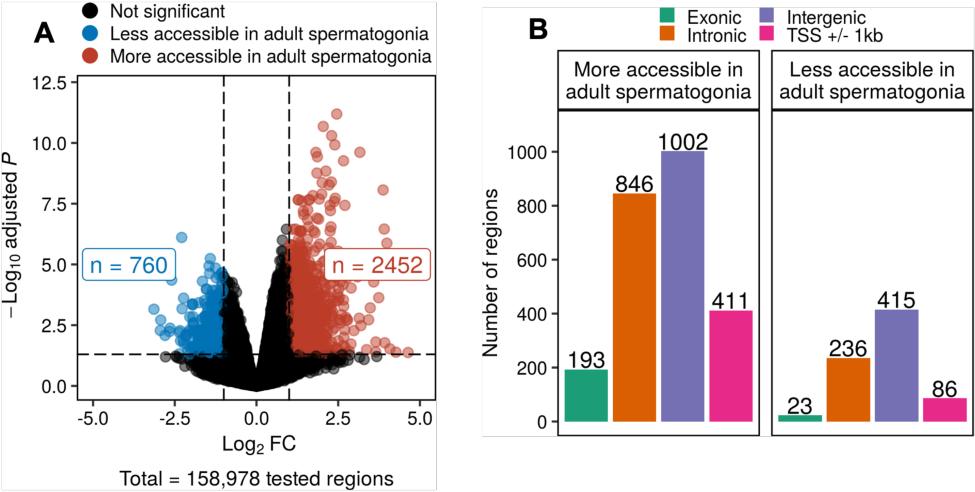
\includegraphics{thesis_files/figure-latex/df1a-1} 

}

\caption[Regions of differential chromatin accessibility in spermatogonial cells between postnatal and adult stages]{\textbf{Regions of differential chromatin accessibility in spermatogonial cells between postnatal and adult stages associate with distinct biological processes.}\newline \textbf{A:} Volcano plot of differentially accessible regions (adjusted P $\leq$ 0.05 and absolute Log\textsubscript{2} FC $\geq$ 1) between PND15 (n = 6) and adult (n = 5) spermatogonial cells identified by ATAC-seq.\newline \textbf{B:} Bar plot illustrating the genomic distribution of differentially accessible chromatin regions in PND15 and adult spermatogonial cells. Genomic regions are categorized in exonic, intronic, intergenic and +/- 1kb from the TSS of a gene.}\label{fig:df1a}
\end{figure}

\begin{figure}[htbp]

{\centering 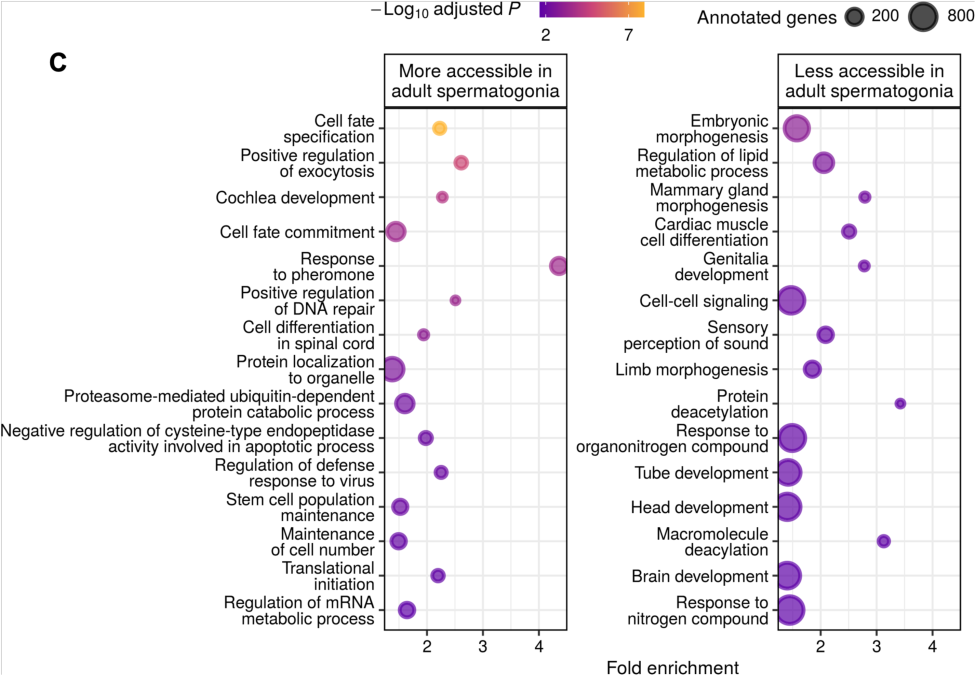
\includegraphics{thesis_files/figure-latex/df1b-1} 

}

\caption[Regions of differential chromatin accessibility in spermatogonial cells between postnatal and adult stages]{\textbf{Regions of differential chromatin accessibility in spermatogonial cells between postnatal and adult stages associate with distinct biological processes.}\newline \textbf{C:} Dot plots of top enriched GO biological processes for regions with increased or decreased chromatin accessibility in adult spermatogonia. Dots size indicates the number of genes in the term, and their colour corresponds to the adjusted P-value of the term’s enrichment.}\label{fig:df1b}
\end{figure}
\end{subfigures}
\begin{subfigures}


\begin{figure}[htbp]

{\centering 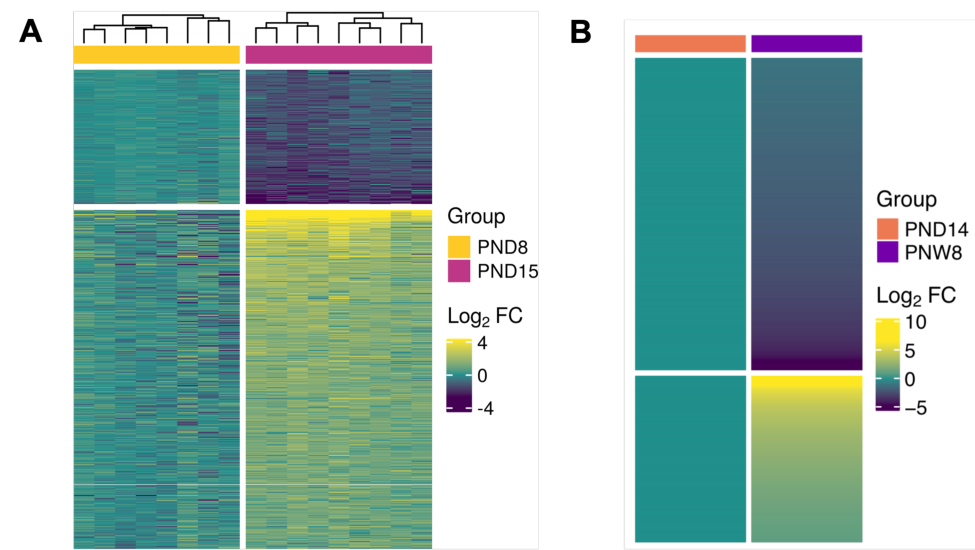
\includegraphics{thesis_files/figure-latex/df2a-1} 

}

\caption[Transcriptomic profile in postnatal and adult spermatogonial cells]{\textbf{Transcriptomic profile in postnatal and adult spermatogonial cells.}\newline \textbf{A:} Heatmap of differentially expressed genes (coding and non-coding) (adjusted P $\leq$ 0.05 and absolute Log\textsubscript{2} FC $\geq$ 1) between PND8 (n = 9) and PND15 (n = 8) spermatogonial cells. Shown are Log\textsubscript{2} FC with respect to the average of PND8 data. Samples are clustered using Ward’s method. Genes are ordered by principal component analysis (PCA) method using seriation (R package).\newline \textbf{B:} Dot plots of top 20 enriched GO biological processes  (adjusted P $\leq$ 0.05) from GSEA analysis of PND8 versus PND15. GO terms are summarized by REVIGO and ordered by their normalized enrichment scores (NES). The size of the dot indicates the number of expressed genes annotated in the GO term, and the colour corresponds to the adjusted P-value.}\label{fig:df2a}
\end{figure}

\begin{figure}[htbp]

{\centering 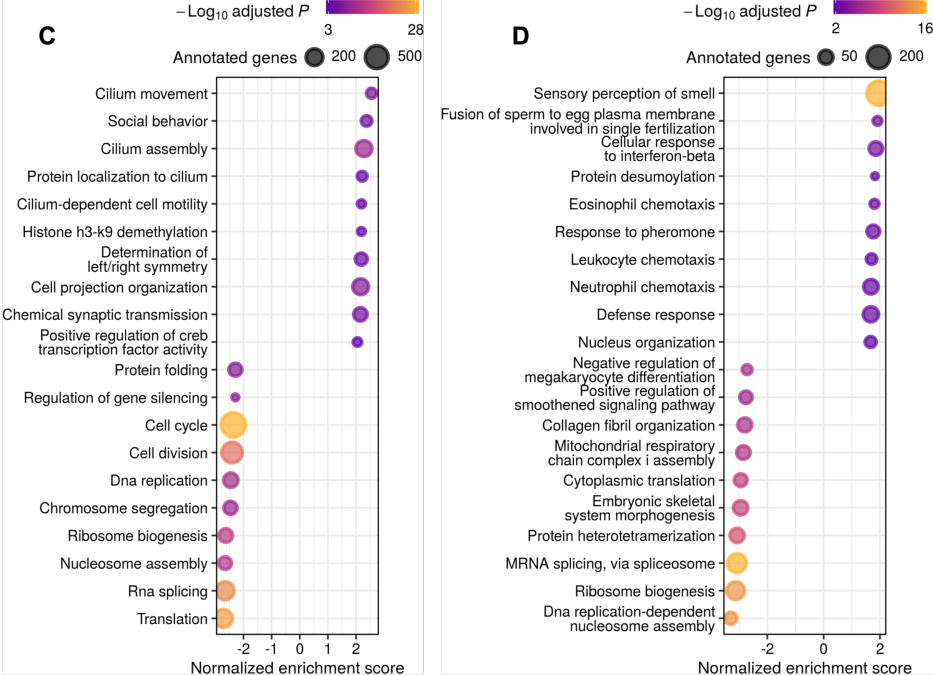
\includegraphics{thesis_files/figure-latex/df2b-1} 

}

\caption[Transcriptomic profile in postnatal and adult spermatogonial cells]{\textbf{Transcriptomic profile in postnatal and adult spermatogonial cells.} \newline \textbf{C,D:} Dot plots of top 10 enriched GO BP terms (adjusted P $\leq$ 0.05) from GSEA analysis of PND15 vs PND8 and PNW8 vs PND14 comparison, respectively. GO terms are summarized by REVIGO and ordered by their normalized enrichment scores (NES). The size of the dot indicates the number of expressed genes annotated in the GO term, and the colour corresponds to the adjusted P value.}\label{fig:df2b}
\end{figure}
\end{subfigures}
\begin{subfigures}


\begin{figure}[htbp]

{\centering 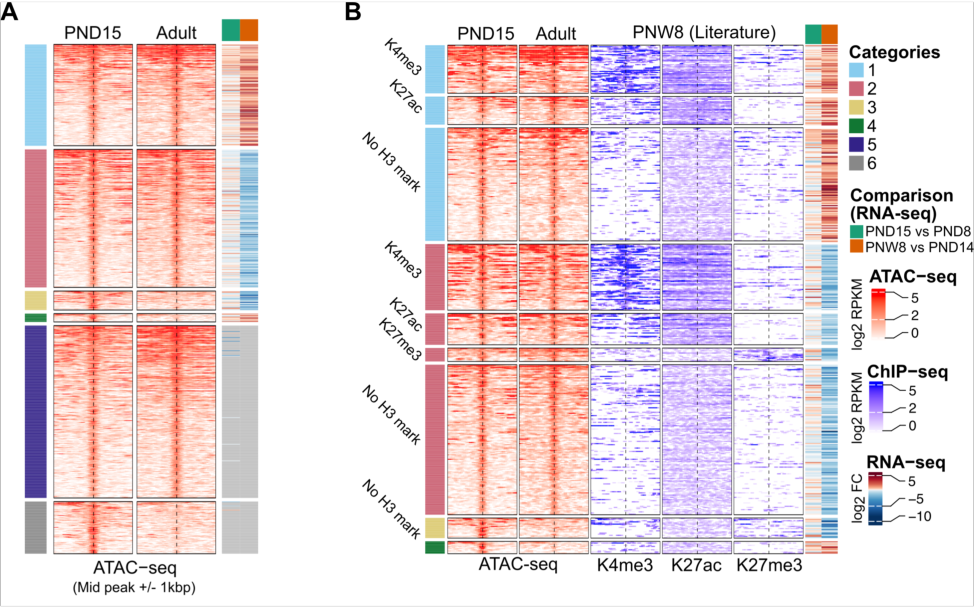
\includegraphics{thesis_files/figure-latex/df3a-1} 

}

\caption[Chromatin accessibility and histone modifications at proximal regions of genes dynamically expressed between PND15 and adult spermatogonial cells]{\textbf{Chromatin accessibility and histone modifications at proximal regions of genes dynamically expressed between PND15 and adult spermatogonial cells.} \newline \textbf{A:} Heatmap of mean coverage across conditions showing proximal regions of increased chromatin accessibility and increased (Category 1, n = 171) or decreased (Category 2, n = 233) gene expression, decreased chromatin accessibility and decreased (Category 3, n = 32) or increased (Category 4, n = 14) gene expression when comparing PND15 with adult spermatogonia. Proximal inactive regions were defined as regions with increased (Category 5, n = 291) or decreased (Category 6, n = 88) accessibility for which no expression of the nearest gene could be detected by RNA-seq. \newline \textbf{B:} Heatmap showing the overlap between Category 1-4 regions and ChIP-seq data in PNW8 spermatogonia for H3K4me3, H3K27ac and H3K27me3. For each of the Category 1-4, the following sub-categorization was applied: regions enriched for H3K4me3 (with or w/o H3K27ac and/or H3K27me3), regions enriched for H3K27ac (and lack both H3K4me3 and H3K27me3) and regions enriched for H3K27me3 (and lack both H3K4me3 and H3K27ac). For (\textbf{A}, \textbf{B}), each line represents a peak region and regions are ordered within a category by the ATAC-seq signal. Mid-x-axis corresponds to the middle of a peak region and is extended to +/- 1 kb. The colour-key of the ATAC-seq heatmap represents the ATAC-seq signal in Log\textsubscript{2} Reads Per Kilobase per Million (RPKM) reads sequenced. For RNA-seq, Log\textsubscript{2} FC is shown from PND8 versus PND15 and PND14 versus PNW8 comparisons. Rows are ordered by the enriched scores of ATAC-seq data.}\label{fig:df3a}
\end{figure}

\begin{figure}[htbp]

{\centering 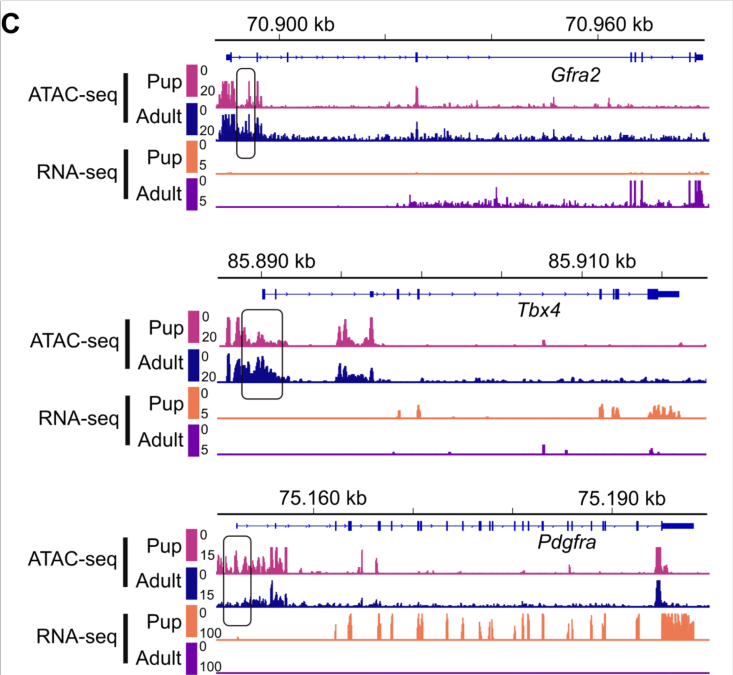
\includegraphics{thesis_files/figure-latex/df3b-1} 

}

\caption[Chromatin accessibility and histone modifications at proximal regions of genes dynamically expressed between PND15 and adult spermatogonial cells]{\textbf{Chromatin accessibility and histone modifications at proximal regions of genes dynamically expressed between PND15 and adult spermatogonial cells.} \newline \textbf{C:} Genomic snapshots from the Integrative Genomics Viewer (IGV, Broad Institute) of exemplary genes from Category 1 (Gfra2), category 2 (Hmx1) and category 3 (Pdgfra) showing the relative abundance of transcripts from RNA-seq and chromatin accessibility from ATAC-seq. RNA-seq data correspond to literature PND14 and PNW8 spermatogonial cells and ATAC-seq data to PND15 and adult spermatogonial cells. Genomic snapshots from the Integrative Genomics Viewer (IGV, Broad Institute) of exemplary genes from Category 1 (Gfra2), Category 2 (Hmx1) and Category 3 (Pdgfra) showing the relative abundance of transcripts from RNA-seq, chromatin accessibility from ATAC-seq and enrichment of 3 different histone marks (H3K27ac, H3K4me3 and H3K27me3) from ChIP-seq. Pup (PND15 ATAC-seq or PND14 RNA-seq samples) spermatogonia are represented in green and adult (PNW20 ATAC-seq samples or PNW8 RNA-seq and ChIP-seq samples) spermatogonia are represented in orange and overlayed in each of the IGV tracks.}\label{fig:df3b}
\end{figure}
\end{subfigures}
\begin{subfigures}

\begin{figure}[htbp]

{\centering 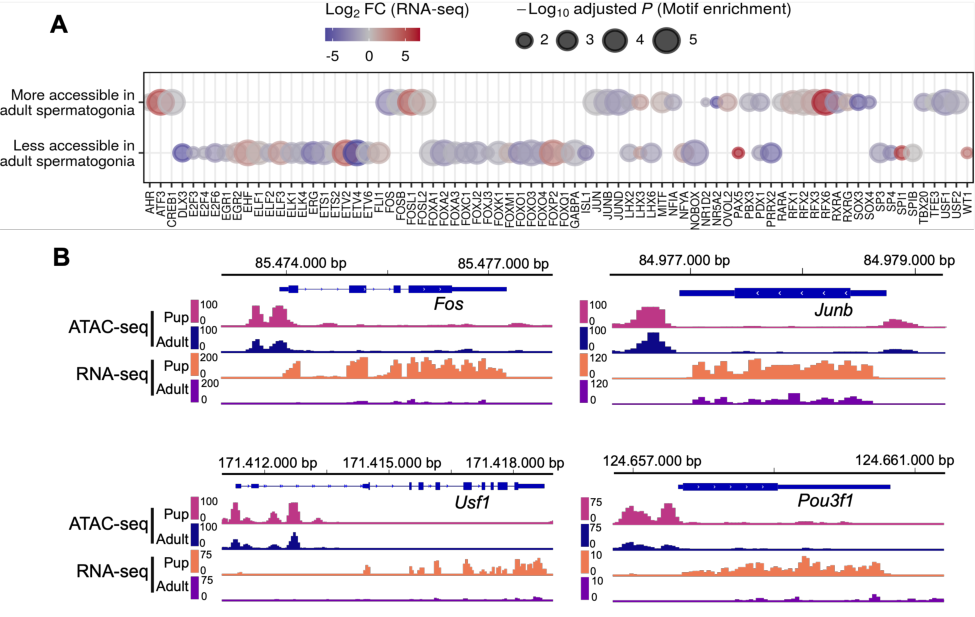
\includegraphics{thesis_files/figure-latex/df4a-1} 

}

\caption[Transcription factor dynamics at differentially accessible regions is predicted by motif enrichment in adult spermatogonial cells]{\textbf{Transcription factor dynamics at differentially accessible regions is predicted by motif enrichment in adult spermatogonial cells.} \newline \textbf{A:} Dot plot of all transcription factor motifs enriched in the regions of decreased and increased accessibility between adult and PND15 spermatogonia. Each dot corresponds to a motif. The differential gene expression of each transcription factor was extracted from the PND14 and PNW8 literature RNA-seq and is shown as colour-coded Log\textsubscript{2} FC. The size of the dot indicates the HOMER motif enrichment adjusted P of each motif. \newline \textbf{B:} Genomic snapshots from the Integrative Genomics Viewer (IGV, Broad Institute) of mRNA expression levels of representative enriched TFs in the regions of increased chromatin accessibility. RNA-seq data corresponds to literature PND14 and adult (PNW8) spermatogonial cells and  ATAC-seq data to PND15 and adult (PNW20) spermatogonial cells, respectively.}\label{fig:df4a}
\end{figure}

\begin{figure}[htbp]

{\centering 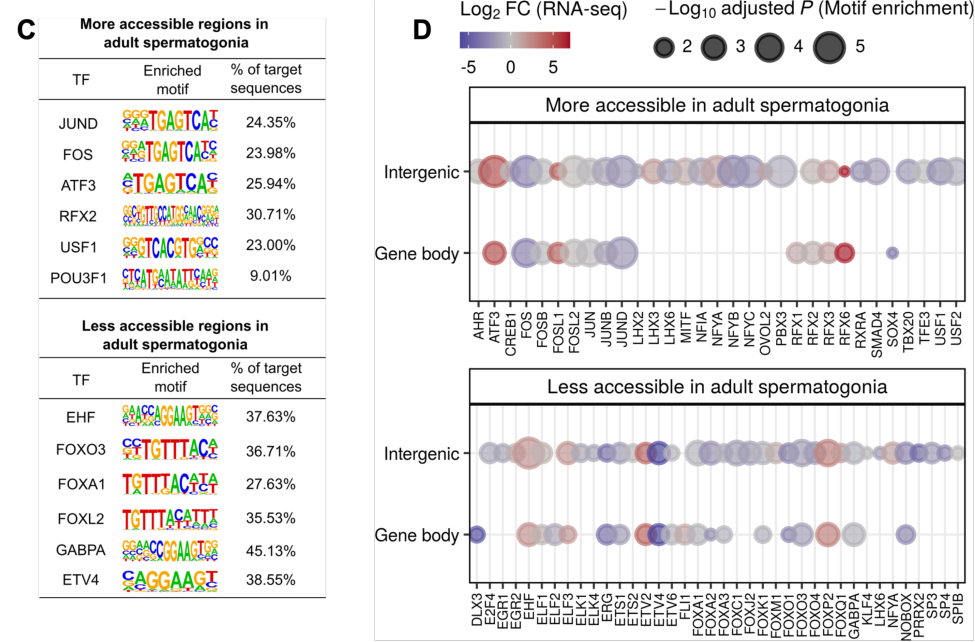
\includegraphics{thesis_files/figure-latex/df4b-1} 

}

\caption[Transcription factor dynamics at differentially accessible regions is predicted by motif enrichment in adult spermatogonial cells]{\textbf{Transcription factor dynamics at differentially accessible regions is predicted by motif enrichment in adult spermatogonial cells.} \newline \textbf{C:} HOMER extracted consensus sequences for each transcription factor motif. Representative examples from the most enriched transcription factor families are depicted. \newline \textbf{D:} Dot plots of top transcription factor motifs enriched in differentially accessible chromatin regions situated in gene bodies and in intergenic areas of the genome. Each dot corresponds to a motif. The differential gene expression of each transcription factor was extracted from the PND14 and PNW8 literature RNA-seq and is shown as colour-coded Log\textsubscript{2} FC. The size of the dot indicates the HOMER motif enrichment adjusted P of each motif.}\label{fig:df4b}
\end{figure}
\end{subfigures}
\begin{subfigures}


\begin{figure}[htbp]

{\centering 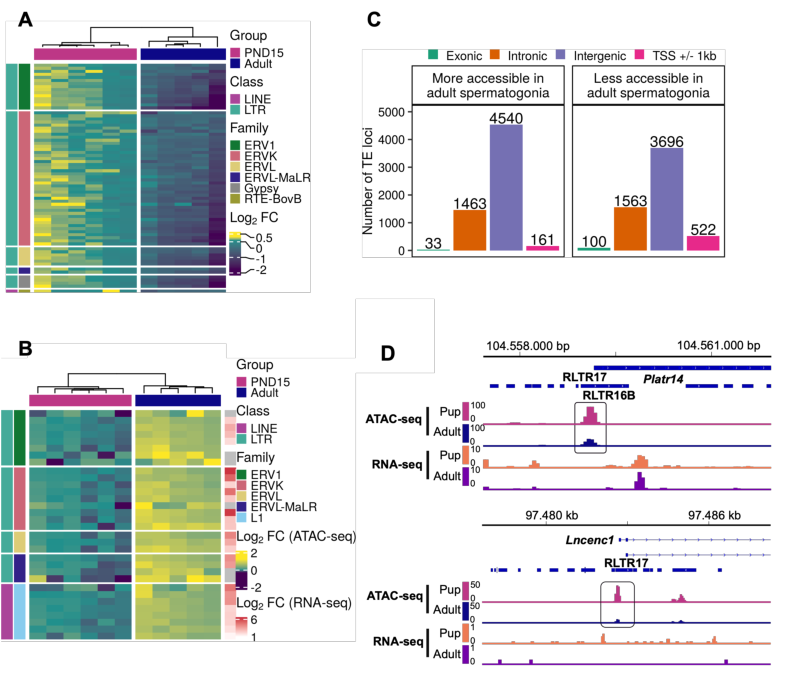
\includegraphics{thesis_files/figure-latex/df5a-1} 

}

\caption[Differential chromatin accessibility at transposable elements (TEs) in adult spermatogonial cells compared to PND15]{\textbf{Differential chromatin accessibility at transposable elements (TEs) in adult spermatogonial cells compared to PND15.} \newline \textbf{A:} Heatmap of the LTR and LINE subtypes with decreased accessibility between adult and PND15 spermatogonia (adjusted P $\leq$ 0.05 and Log\textsubscript{2} FC $\geq$ 0.5). \newline \textbf{B:} Heatmap of the LTR and LINE subtypes with increased accessibility between adult and PND15 spermatogonia (adjusted P $\leq$ 0.05 and Log\textsubscript{2} FC $\geq$ 0.5). Expression changes of these subtypes between PNW8 and PND14 spermatogonia literature RNA-seq is represented as Log\textsubscript{2} FC. \newline (\textbf{A}, \textbf{B}) Log\textsubscript{2} FC are shown with respect to the average of the PND15 samples. Samples are clustered using Ward’s method. Subtypes are ordered by principal component analysis (PCA) method using seriation (R package). \newline \textbf{C:} Bar plot illustrating the genomic distribution of differentially accessible TEs between adult and PND15 spermatogonial cells. \newline \textbf{D:} Genomic snapshots from the Integrative Genomics Viewer (IGV, Broad Institute) of Lncenc1 and Platr14 showing LTRs from RepeatMasker and the average normalized RNA-seq and ATAC-seq coverage (RPKM). LTR loci were extracted using RepeatMasker. RNA-seq data corresponds to literature PND14 and adult (PNW8) spermatogonial cells and  ATAC-seq data to PND15 and adult (PNW20) spermatogonial cells, respectively.}\label{fig:df5a}
\end{figure}


\begin{figure}[htbp]

{\centering 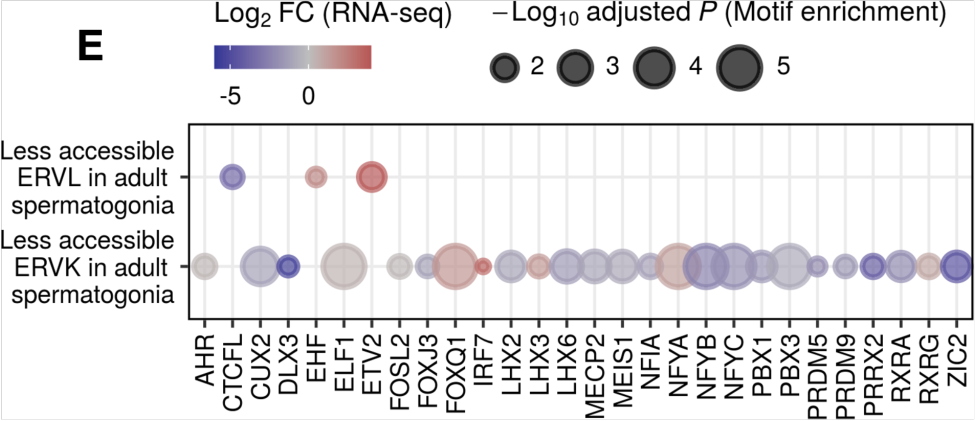
\includegraphics{thesis_files/figure-latex/df5b-1} 

}

\caption[Differential chromatin accessibility at transposable elements (TEs) in adult spermatogonial cells compared to PND15]{ \textbf{Differential chromatin accessibility at transposable elements (TEs) in adult spermatogonial cells compared to PND15.} \newline \textbf{E:} Dot plots of top transcription factor motifs enriched in the less accessible ERVKs and ERVL subtypes. Each dot corresponds to a motif. The differential gene expression of each transcription factor was extracted from the PNW8 vs PND14 comparison from literature RNA-seq and is shown as colour-coded Log\textsubscript{2} FC. The size of the dot indicates the HOMER motif enrichment adjusted P of each motif.}\label{fig:df5b}
\end{figure}
\end{subfigures}

\begin{figure}[htbp]

{\centering 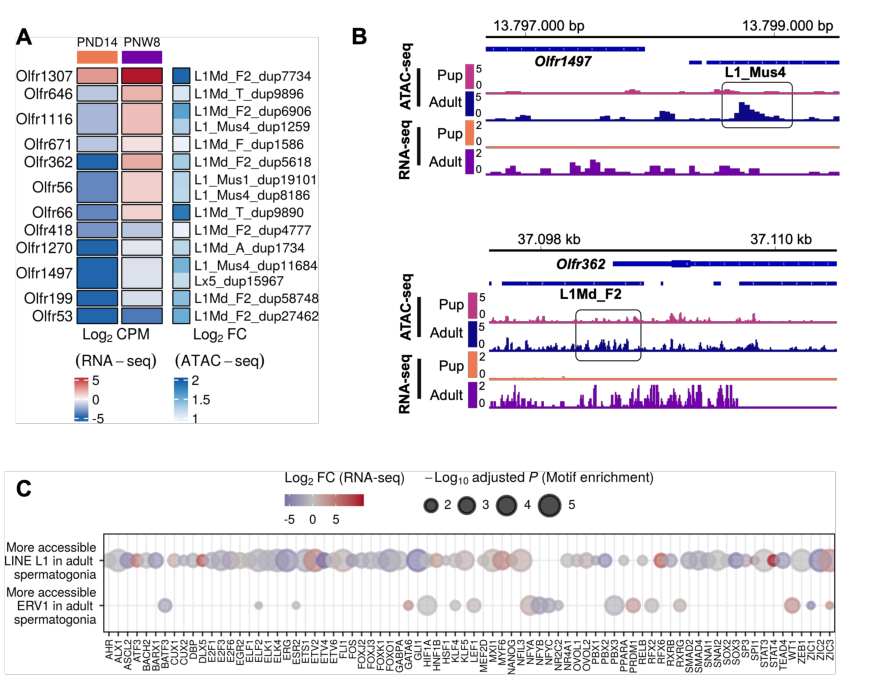
\includegraphics{thesis_files/figure-latex/df6-1} 

}

\caption[Increased accessibility at LINE L1 subtypes located near Olfr gene clusters]{\textbf{Increased accessibility at LINE L1 subtypes located near Olfr gene clusters.} \newline \textbf{A:} Heatmap of the Olfr genes for which we identified an upregulated expression from PND14 to PNW8 timepoints and an increase in accessibility at a nearby L1 locus. RNA expression levels are expressed as Log\textsubscript{2} CPM at each timepoint. Accessibility changes at each of the corresponding L1 locus situated within +/- 5kbp from the gene are expressed as Log\textsubscript{2} FC calculated from the ATAC-seq analysis of the differentially accessible TEs between adult and PND15 spermatogonial cells. Locus are ordered by PCA method using seriation (R package). \newline \textbf{B:} Genomic snapshots from the Integrative Genomics Viewer (IGV, Broad Institute) of exemplary genes Olfr1497 and Olfr362 showing relative abundance of transcripts from RNA-seq and chromatin accessibility from ATAC-seq. LINE loci were extracted using Repeat Masker. RNA-seq data corresponds to literature PND14 and adult (PNW8) spermatogonial cells and ATAC-seq data to PND15 and adult (PNW20) spermatogonial cells, respectively. \newline \textbf{C:} Dot plots of top transcription factor motifs enriched in the more accessible L1 and ERV1 subtypes. Each dot corresponds to a motif. The differential gene expression of each transcription factor was extracted from the PNW8 vs PND14 comparison from literature RNA-seq and is shown as colour-coded Log\textsubscript{2} FC. The size of the dot indicates the HOMER motif enrichment adjusted P of each motif.}\label{fig:df6}
\end{figure}
\hypertarget{supplementary-figures}{%
\section{Supplementary Figures}\label{supplementary-figures}}
\begin{subfigures}


\begin{figure}[htbp]

{\centering 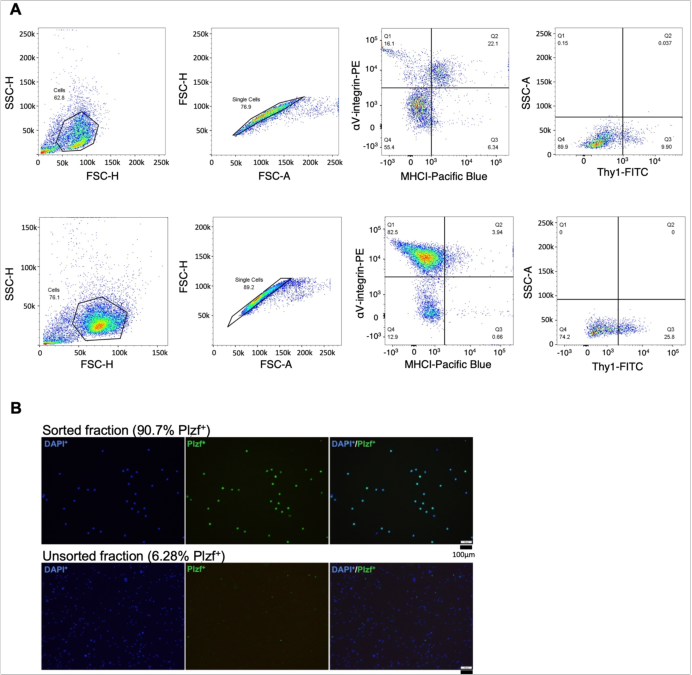
\includegraphics{thesis_files/figure-latex/ds1a-1} 

}

\caption[FACS leads to enrichment of PLZF+ cells in testicular preparations from mouse]{\textbf{FACS leads to enrichment of PLZF+ cells in testicular preparations from mouse.} \newline \textbf{A:} Representative dot plots of the sorting strategy for spermatogonial cell enrichment. Gating based on side scatter/forward scatter (SSC-A/FSC-A) and forward scatter – height/ forward scatter – area (FSC-H/FSC-A) was performed to exclude cell debris and cell clumps. \newline \textbf{B:} PLZF+ cells are enriched following FACS, illustrated by immunocytochemistry on unsorted and sorted cell preparations. Immunocytochemistry of PND15 unsorted and the sorted testis cell suspension was performed by fixating cells on poly-L-lysine coated slides. Cells were stained with anti-PLZF antibody (S19 clone, Active Motif) and VECTASHIELD (with DAPI) antifade mounting medium was used for mounting. Cells were visualized with a fluorescence microscope and counted in 10 different fields of view/slide. The number of PLZF+ and PLZF- cells from 10 different fields of view were averaged.}\label{fig:ds1a}
\end{figure}

\begin{figure}[htbp]

{\centering 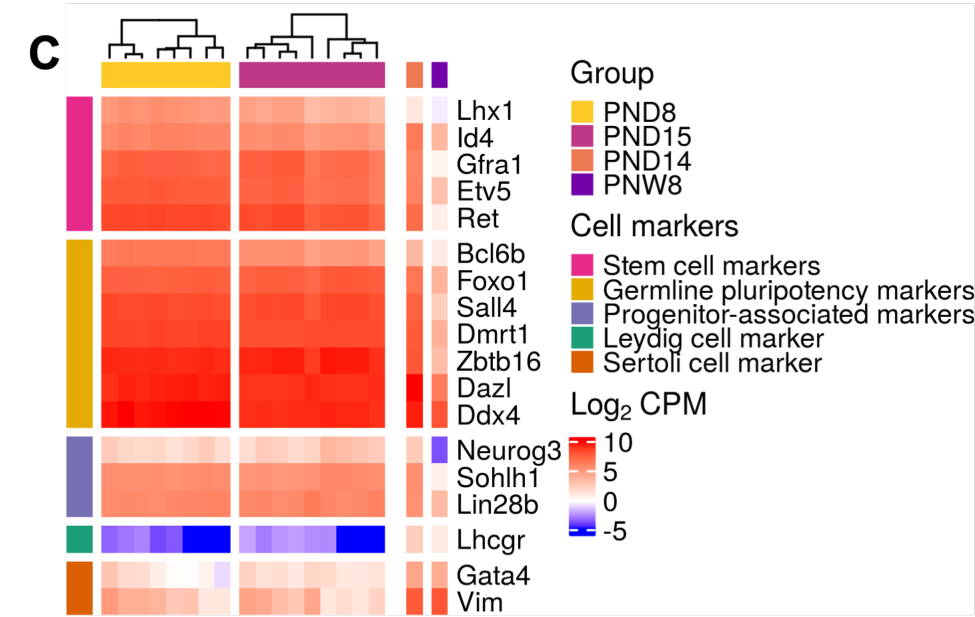
\includegraphics{thesis_files/figure-latex/ds1b-1} 

}

\caption[FACS leads to enrichment of PLZF+ cells in testicular preparations from mouse]{\textbf{FACS leads to enrichment of PLZF+ cells in testicular preparations from mouse.} \newline \textbf{C} Heatmap of the expression profile of selected markers for spermatogonial and different testicular somatic cells from our PND8 and PND15  RNA-seq data, and PND14 and PNW8 datasets from the literature. Key genes for stem cell potential, stem and progenitor spermatogonia, and Leydig and Sertoli cells were chosen to evaluate spermatogonial cells enrichment in the populations. Gene expression is represented in Log\textsubscript{2}CPM (counts per million).}\label{fig:ds1b}
\end{figure}
\end{subfigures}
\begin{subfigures}


\begin{figure}[htbp]

{\centering 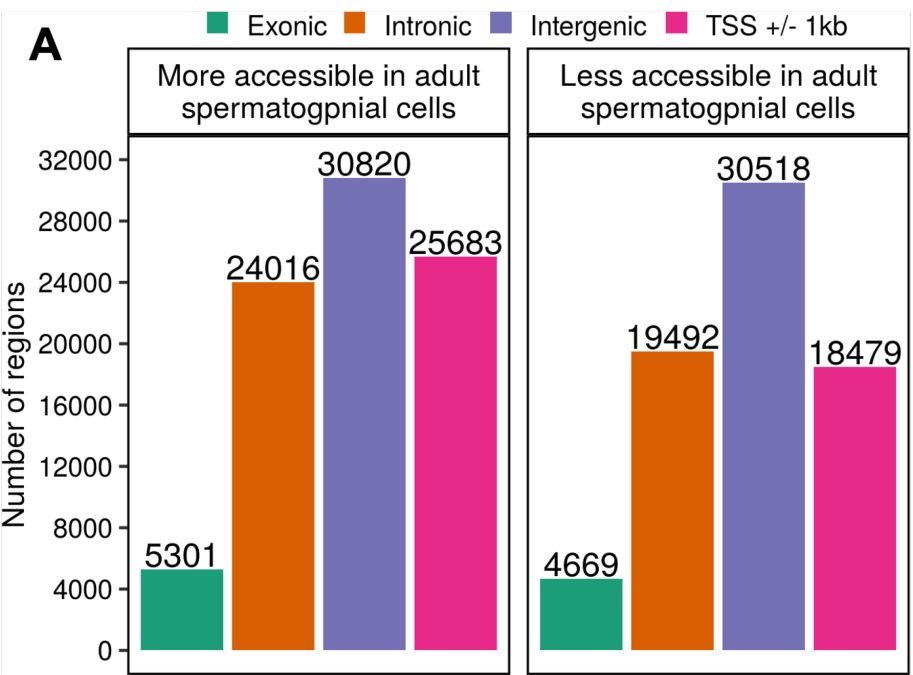
\includegraphics{thesis_files/figure-latex/ds2a-1} 

}

\caption[Omni-ATAC profiles of PND15 and adult spermatogonial cells and their genomic distribution]{\textbf{Omni-ATAC profiles of PND15 and adult spermatogonial cells and their genomic distribution.} \newline \textbf{A:} Genomic distribution of the 158, 978 identified Omni-ATAC regions in between exonic, intronic, intergenic and located +/- 1kb of a transcriptional start site (TSS).}\label{fig:ds2a}
\end{figure}

\begin{figure}[htbp]

{\centering 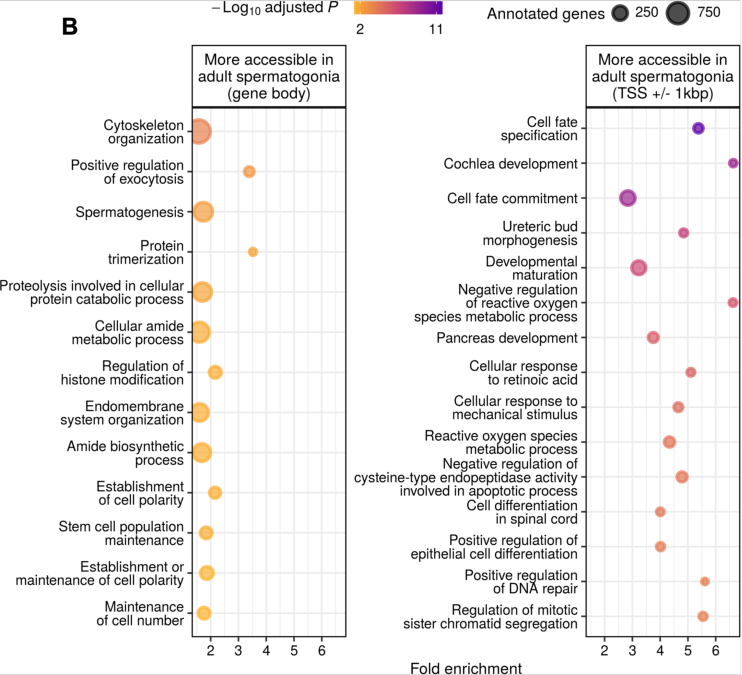
\includegraphics{thesis_files/figure-latex/ds2b-1} 

}

\caption[Omni-ATAC profiles of PND15 and adult spermatogonial cells and their genomic distribution]{\textbf{Omni-ATAC profiles of PND15 and adult spermatogonial cells and their genomic distribution.} \newline \textbf{B:} Dot plots of top enriched GO biological processes for regions with increased chromatin accessibility in adult spermatogonia, within gene bodies and around TSS of nearby genes (TSS +/- 1kb). The size of dots indicates the number of genes in the term and the colour of each dot corresponds to the adjusted P-value of the term’s enrichment.}\label{fig:ds2b}
\end{figure}
\end{subfigures}

\begin{figure}[htbp]

{\centering 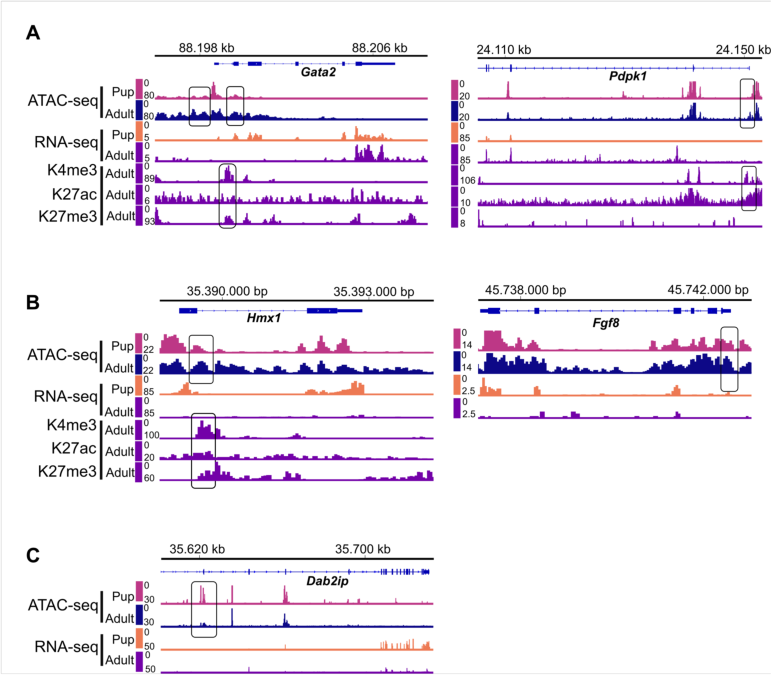
\includegraphics{thesis_files/figure-latex/ds3-1} 

}

\caption[Representative examples from Categories 1-3 resulted from the overlap of chromatin accessibility, gene expression and histone profiling datasets]{\textbf{Representative examples from Categories 1-3 resulted from the overlap of chromatin accessibility, gene expression and histone profiling datasets.} Genomic snapshots from the Integrative Genomics Viewer (IGV, Broad Institute) of exemplary genes from \textbf{A:} Category 1 (Pdpk1 and Gata2), \textbf{B:} Category 2 (Hmx1 and Fgf8), and \textbf{C:} Category 3 (Dap2ip) showing the relative abundance of transcripts from RNA-seq, chromatin accessibility from ATAC-seq and enrichment of H3K27ac, H3K4me3 and H3K27me3 from ChIP-seq. RNA-seq data correspond to literature PND14 and PNW8 spermatogonial cells and ATAC-seq data to PND15 and adult spermatogonial cells.}\label{fig:ds3}
\end{figure}

\begin{figure}[htbp]

{\centering 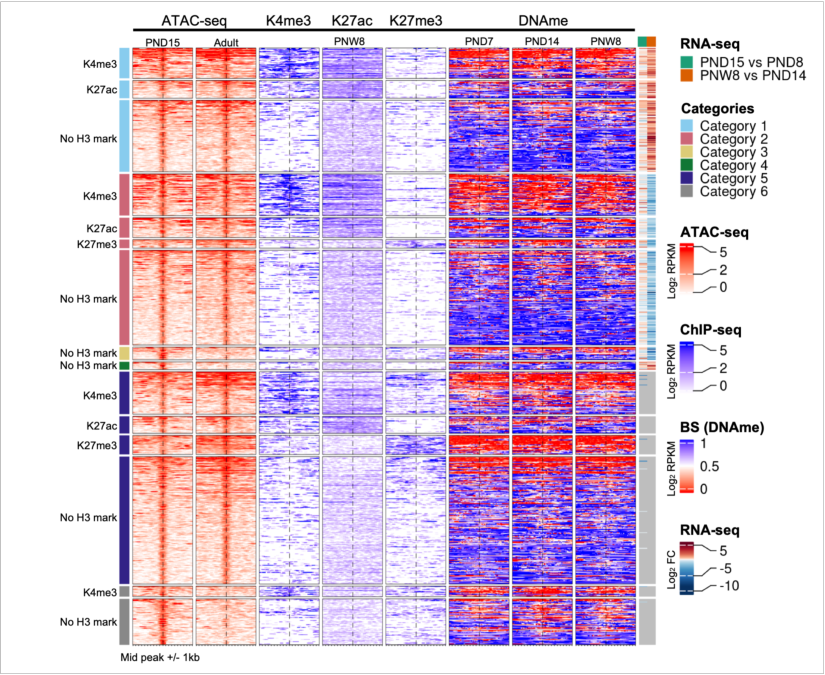
\includegraphics{thesis_files/figure-latex/ds4-1} 

}

\caption[DNAme profiles of spermatogonial cells do not show major changes over the period of testis postnatal maturation]{\textbf{DNAme profiles of spermatogonial cells do not show major changes over the period of testis postnatal maturation.} Enriched heatmaps showing the overlap between Category 1-4 regions, literature ChIP-seq data in PNW8 spermatogonia for H3K4me3, H3K27ac and H3K27me3, and DNAme data from BS in PND7, PND14 and PNW8 spermatogonia. For each of the Category 1-4 the following sub-categorization was applied: regions that are enriched for H3K4me3 (with or w/o H3K27ac and/or H3K27me3), regions that are enriched for H3K27ac (and lack both H3K4me3 and H3K27me3) and regions that are enriched for H3K27me3 (and lack both H3K4me3 and H3K27ac). Each line represents a peak region and the regions are ordered by the ATAC-seq signal. Mid-x-axis corresponds to the middle of a peak region and is extended to +/- 1 kbp. The colour-key of the ATAC-seq, ChIP-seq and BS heatmaps represent ATAC-seq, ChIP-seq and BS signal, respectively. For RNA-seq, Log\textsubscript{2} FC is shown from PND8 vs PND15 and PND14 vs PNW8 comparisons. For BS, the level of DNAme is between 0 and 1, with 0 representing completely unmethylated loci and 1 fully methylated loci, respectively.}\label{fig:ds4}
\end{figure}

\begin{figure}[htbp]

{\centering \includegraphics{thesis_files/figure-latex/ds5-1} 

}

\caption[Distinct chromatin profiles between PND15 and adult spermatogonia are present at distal regions across the genome]{\textbf{Distinct chromatin profiles between PND15 and adult spermatogonia are present at distal regions across the genome.} \textbf{(A-B)} Enriched heatmaps showing the overlap between more accessible regions \textbf{(A)} and less accessible regions \textbf{(B)} situated in distal regions in spermatogonial cells, and literature ChIP-seq and DNAme data in PNW8 spermatogonia. The following sub-categorization was applied: regions that are enriched for H3K4me3 (with or w/o H3K27ac and/or H3K27me3), regions that are enriched for H3K27ac (and lack both H3K4me3 and H3K27me3) and regions that are enriched for H3K27me3 (and lack both H3K4me3 and H3K27ac). Each line represents a peak region and the regions are ordered by the ATAC-seq signal. Mid-x-axis corresponds to the middle of a peak region and is extended to +/- 1 kbp. The colour-key of the ATAC-seq, ChIP-seq and BS heatmaps represent ATAC-seq, ChIP-seq and BS signal, respectively. For BS, the level of DNAme is between 0 and 1, with 0 representing completely unmethylated loci and 1 fully methylated loci, respectively.}\label{fig:ds5}
\end{figure}

\begin{figure}[htbp]

{\centering 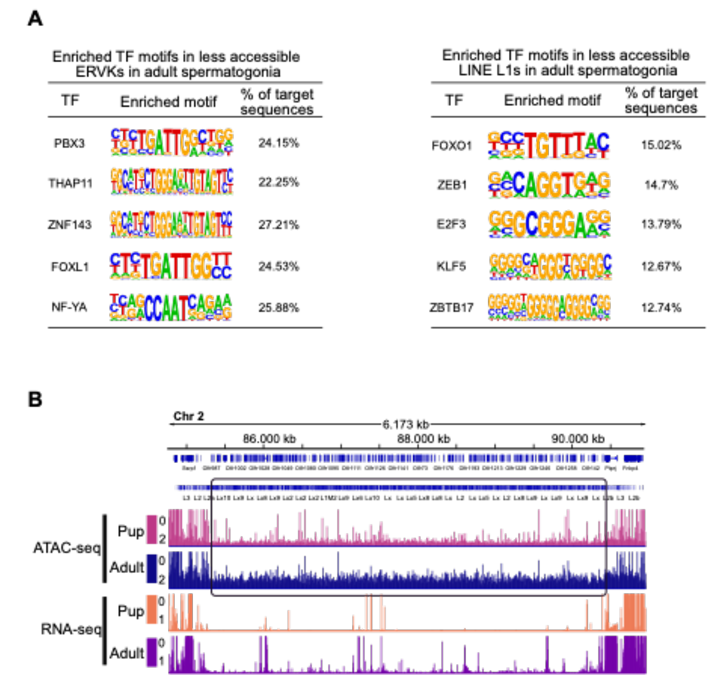
\includegraphics{thesis_files/figure-latex/ds6-1} 

}

\caption[Differentially accessible TEs exhibit enriched TF motifs and correspond to regions nearby non-random gene families]{\textbf{Differentially accessible TEs exhibit enriched TF motifs and correspond to regions nearby non-random gene families.} \textbf{A:} HOMER extracted consensus sequences for TF motifs enriched in less accessible ERVK subtypes. Representative examples from the most enriched transcription factor families are depicted. \textbf{B:} Genomic snapshots from the Integrative Genomics Viewer (IGV, Broad Institute) of a cluster of Olfr genes on Chr2 overlapping an increased density of LINE elements relative to the neighbouring regions. The relative abundance of transcripts from RNA-seq and chromatin accessibility from ATAC-seq are shown. RNA-seq data corresponds to literature PND14 and adult (PNW8) spermatogonial cells and ATAC-seq data to PND15 and adult (PNW20) spermatogonial cells, respectively.}\label{fig:ds6}
\end{figure}
\newpage

\hypertarget{st}{%
\section{Supplementary tables}\label{st}}

Supplementary tables are too big to be included in the thesis, hence they are provided as links
\begin{enumerate}
\def\labelenumi{\arabic{enumi}.}
\tightlist
\item
  \href{../../figures/dev/t1.xlsx}{Supplementary table 1}
\item
  \href{../../figures/dev/t2.xlsx}{Supplementary table 1}
\item
  \href{../../figures/dev/t3.xlsx}{Supplementary table 1}
\item
  \href{../../figures/dev/t4.xlsx}{Supplementary table 1}
\item
  \href{../../figures/dev/t5.xlsx}{Supplementary table 1}
\item
  \href{../../figures/dev/t6.xlsx}{Supplementary table 1}
\end{enumerate}
\chaptermark{Chapter 2}

\hypertarget{chapter2}{%
\chapter{Early life stress affects the miRNA cargo of epididymal extracellular vesicles in mouse}\label{chapter2}}

Anar Alshanbayeva\textsuperscript{1,2,3}, \textbf{Deepak K
Tanwar}\textsuperscript{1,2,3}, Martin
Roszkowski\textsuperscript{1,2,3}, Francesca
Manuella\textsuperscript{1,2,3}, Isabelle M
Mansuy\textsuperscript{1,2,3,\#} \newline \newline
\textsuperscript{1}Laboratory of Neuroepigenetics, Brain Research
Institute at the Medical Faculty of the University of Zurich. \newline
\textsuperscript{2}Institute for Neuroscience of the Department of
Health Sciences and Technology, ETH Zurich, Zurich, Switzerland.
\newline \textsuperscript{3}Zurich Neuroscience Center, ETH and
University of Zurich, Zurich, Switzerland. \newline \newline
\textsuperscript{\#}Corresponding author \newline \newline
\textbf{Journal:} \emph{Biology of Reproduction} \newline \newline 
\textbf{DOI:} \href{https://doi.org/10.1093/biolre/ioab156}{10.1093/biolre/ioab156}
\newline \newline
\textbf{Contributions:} \emph{I performed data analysis with Anar Alshanbayeva,
generated figures with Anar Alshanbayeva, assisted Anar Alshanbayeva in
writing the manuscript, and revised manuscript with Anar Alshanbayeva.}

\newpage

\hypertarget{graphical-abstract-1}{%
\section{Graphical Abstract}\label{graphical-abstract-1}}
\begin{figure}[htbp]

{\centering 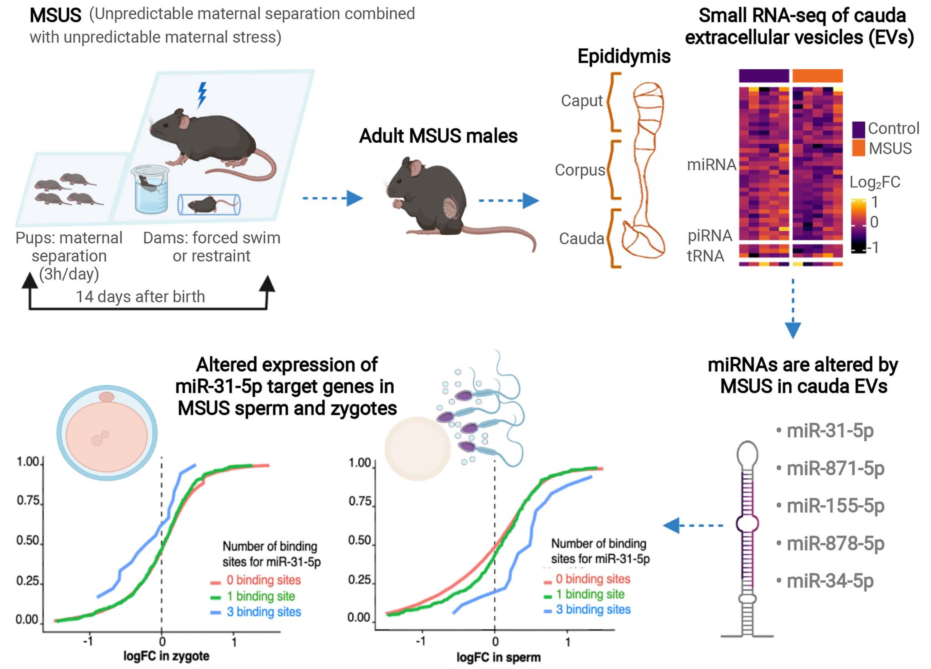
\includegraphics{thesis_files/figure-latex/cf1-1} 

}

\caption[Graphical abstract]{Graphical abstract.}\label{fig:cf1}
\end{figure}
\newpage

\hypertarget{abstract-1}{%
\section{Abstract}\label{abstract-1}}

Sperm RNA can be modified by environmental factors and has been
implicated in communicating signals about changes in a father's
environment to the offspring. The small RNA composition of sperm could
be changed during its final stage of maturation in the epididymis by
extracellular vesicles (EVs) released by epididymal cells. We studied
the effect of exposure to stress in early postnatal life on the
transcriptome of epididymal EVs using a mouse model of transgenerational
transmission. We found that the small RNA signature of epididymal EVs,
particularly miRNAs, is altered in adult males exposed to postnatal
stress. In some cases, these miRNA changes correlate with differences in
the expression of their target genes in sperm and zygotes generated from
that sperm. These results suggest that stressful experiences in early
life can have persistent biological effects on the male reproductive
tract that may in part be responsible for the transmission of the
effects of exposure to the offspring.

\hypertarget{summary-sentence}{%
\section{Summary sentence}\label{summary-sentence}}

miRNA cargo of extracellular vesicles in cauda epididymis is altered by
paternal exposure to early life stress. This correlates with changes in
the expression of target genes in sperm and in zygotes generated from
that sperm.

\hypertarget{key-words}{%
\section{Key words}\label{key-words}}

epigenetics, epididymis, epididymosomes, early life stress,
extracellular vesicles, miRNAs, sperm.

\newpage

\hypertarget{introduction-1}{%
\section{Introduction}\label{introduction-1}}

Post-testicular maturation of spermatozoa in the epididymis is an
elaborate process that involves modifications of sperm RNA, protein, and
lipid content (\protect\hyperlink{ref-nixon_2015}{Nixon et al., 2015}; \protect\hyperlink{ref-rejraji_2006}{Rejraji et al., 2006}; \protect\hyperlink{ref-sharma_2016}{Sharma et al., 2016}; \protect\hyperlink{ref-skerget_2015}{Skerget, Rosenow, Petritis, \& Karr, 2015}; \protect\hyperlink{ref-tamessar_2021}{Tamessar et al., 2021}). The epididymis is segmented into different parts,
including the initial segment, caput, corpus, and cauda. Each segment
has a distinct gene expression profile, and different protein and lipid
composition. Some modifications in epididymal spermatozoa are conserved
across species (\protect\hyperlink{ref-sellem_2020}{Sellem et al., 2020}). For example, \textasciitilde50\% of miRNAs, a class of
small RNAs that are modified during caput to cauda epididymis transit,
is identical in mouse and bovine spermatozoa (\protect\hyperlink{ref-sellem_2020}{Sellem et al., 2020}). One
mechanism by which small RNA load in spermatozoa is modified along the
epididymis is by uptake of extracellular vesicles (EVs), also known as
epididymosomes, which are produced by epididymal epithelial cells
(\protect\hyperlink{ref-reilly_2016}{Reilly et al., 2016}). Studies have shown that epididymosomes can be taken up
by maturing sperm through proteins present on the sperm head such as
dynamin in mice and tetraspanins or syntenins in humans
(\protect\hyperlink{ref-caballero_2013}{Caballero, Frenette, Belleannée, \& Sullivan, 2013}; \protect\hyperlink{ref-reilly_2016}{Reilly et al., 2016}; \protect\hyperlink{ref-thimon_2008}{Thimon, Frenette, Saez, Thabet, \& Sullivan, 2008}; \protect\hyperlink{ref-zhou_2019}{Zhou et al., 2019}). Co-incubation
experiments provided evidence for epididymosome-mediated transfer of
miRNAs to spermatozoa (\protect\hyperlink{ref-reilly_2016}{Reilly et al., 2016}). Exogenous DNA and RNA can also be
directly taken up by spermatozoa via artificial liposomes
(\protect\hyperlink{ref-bachiller_1991}{Bachiller, Schellander, Peli, \& Rüther, 1991}).

However, it is still not clear if changes in small RNA composition of
spermatozoa occurring during epididymal transit are required for
embryonic development, and studies on the subject have been conflicting
(\protect\hyperlink{ref-conine_2018}{Conine, Sun, Song, Rivera-Pérez, \& Rando, 2018}; \protect\hyperlink{ref-suganuma_2005}{Suganuma, Yanagimachi, \& Meistrich, 2005}). Changes in sperm small RNA have
nevertheless been suggested to play a role in the transmission of
information about paternal experiences to the progeny and can influence
their developmental trajectory (\protect\hyperlink{ref-chan_2020}{J. C. Chan et al., 2020}; \protect\hyperlink{ref-gapp_2014}{Katharina Gapp et al., 2014}; \protect\hyperlink{ref-sharma_2016}{Sharma et al., 2016}).
Epididymosomal small RNA content can also be altered by exposure, for
instance, to dietary insult and stress (\protect\hyperlink{ref-chan_2020}{J. C. Chan et al., 2020}; \protect\hyperlink{ref-sharma_2016}{Sharma et al., 2016}). For
instance, epididymosomal miRNAs are changed by exposure to chronic
stress (\protect\hyperlink{ref-chan_2020}{J. C. Chan et al., 2020}) and low-protein diet (\protect\hyperlink{ref-sharma_2016}{Sharma et al., 2016}) in mice.

Transmission of information about paternal exposure to the offspring
depends on the type of exposure, its duration and the developmental
window at which it is applied. To date, little is known about the
long-term effects of early life stress, particularly stress experienced
after birth, on epididymosomal small RNA composition in adulthood, and
whether any changes to this composition can influence gene expression in
sperm and in zygotes generated from that sperm. Using a
transgenerational mouse model of postnatal stress induced by
unpredictable maternal separation combined with unpredictable maternal
stress, unpredictable maternal separation combined with unpredictable
maternal stress (MSUS) (\protect\hyperlink{ref-franklin_2010}{Franklin et al., 2010b}), we show that the miRNA
signature of cauda epididymosomes in adult males is altered by exposure,
and that this alteration, correlates with changes in the expression of
their target genes in sperm and in zygotes.

\hypertarget{results-1}{%
\section{Results}\label{results-1}}

\hypertarget{isolation-of-cauda-epididymosomes-confirmed-by-several-methods}{%
\subsection{Isolation of cauda epididymosomes confirmed by several methods}\label{isolation-of-cauda-epididymosomes-confirmed-by-several-methods}}

To characterize the RNA composition of cauda epididymosomes,
epididymosomes were isolated by high-speed ultracentrifugation from
adult control males and males exposed to MSUS (Figure \ref{fig:ef1}A). MSUS
consists of exposing newborn pups to unpredictable maternal separation
for 3h daily and subjecting dams to unpredictable maternal stress during
separation (\protect\hyperlink{ref-franklin_2010}{Franklin et al., 2010b}). Adult MSUS-exposed and control males were
euthanized and cauda epididymis was collected. Successful isolation of
cauda epididymosomes was confirmed by electron microscopy,
immunoblotting, and nanoparticle-tracking analyses (Figure \ref{fig:ef1}). The
presence and purity of epididymosomes was further validated by staining
with the EV-specific marker CD9 and confirmation of the absence of the
cellular marker Glyceraldehyde 3-phosphate dehydrogenase (GAPDH)
(Figure \ref{fig:ef1}B). Size analysis by nanoparticle-tracking indicated that the
collected particles are 50--300nm in diameter (Figure \ref{fig:ef1}D). Imaging by
transmission electron microscopy showed the typical cup-shaped
structures of epididymosomes (Figure \ref{fig:ef1}C, Supplementary Figure \ref{fig:es1}A)
(\protect\hyperlink{ref-choi_2017}{Choi \& Mun, 2017}). RNA profiling by high-resolution automated electrophoresis
showed enrichment for small RNAs of different length, similar to
previous studies on cauda epididymosomal RNA (Supplementary Figure \ref{fig:es1}B) (\protect\hyperlink{ref-conine_2018}{Conine et al., 2018}; \protect\hyperlink{ref-sharma_2016}{Sharma et al., 2016}).

\hypertarget{the-number-and-size-of-epididymosomes-in-adult-males-are-not-altered-by-postnatal-stress}{%
\subsection{The number and size of epididymosomes in adult males are not altered by postnatal stress}\label{the-number-and-size-of-epididymosomes-in-adult-males-are-not-altered-by-postnatal-stress}}

We next examined the number and size of cauda epididymosomes in adult
MSUS and control males by dynamic light scattering. No significant
difference could be detected between MSUS and control males (Figure \ref{fig:ef2}A
and B). Since most epididymosomal production occurs via apocrine
secretion from principal cells located in caput epididymis, we also
examined the expression of genes involved in EVs exocytosis. We chose
Ras-related protein Rab-5A (\emph{Rab5}) and Ras-related protein Rab-7A
(\emph{Rab7}), which are involved in vesicle trafficking, the soluble NSF
attachment protein (SNARE) family protein vesicle-associated membrane
protein 7 (\emph{Vamp7}) and SNARE recognition molecule synaptobrevin homolog
YKT6 (\emph{Ykt6}), involved in vesicle fusion. No significant change in the
expression of these genes could be detected in caput epididymis between
MSUS and control adult males (Figure \ref{fig:ef2}C). However, we observed a
consistent trend (not statistically significant) for decreased
expression of all genes involved in EVs secretion in caput epididymis of
MSUS mice (Figure \ref{fig:ef2}C).

\hypertarget{mirnas-are-persistently-altered-by-postnatal-stress-in-cauda-epididymosomes}{%
\subsection{miRNAs are persistently altered by postnatal stress in cauda epididymosomes}\label{mirnas-are-persistently-altered-by-postnatal-stress-in-cauda-epididymosomes}}

Epididymosomal small RNAs are known to be affected by changing
environmental conditions in rodents. Small RNAs, like tRNA-derived
fragments (tRFs), miRNAs and more recently rRNA-derived small RNA
fragments are believed to act as messengers of a father's experiences
that can be transferred to the offspring (\protect\hyperlink{ref-chan_2020}{J. C. Chan et al., 2020}; \protect\hyperlink{ref-sharma_2016}{Sharma et al., 2016}; \protect\hyperlink{ref-wang_2021}{Y. Wang et al., 2021}; \protect\hyperlink{ref-zhang_2018}{Yunfang Zhang et al., 2018}). Our previous work showed that early postnatal
stress alters small and long RNA content in sperm of adult males
(\protect\hyperlink{ref-gapp_2014}{Katharina Gapp et al., 2014}; \protect\hyperlink{ref-gapp_2020}{K. Gapp, Steenwyk, et al., 2020}). Since caudal sperm and epididymosomal small RNA
profiles are highly similar (\protect\hyperlink{ref-sharma_2016}{Sharma et al., 2016}), we examined whether small RNA
content of cauda epididymosomes is also altered by postnatal stress. We
extracted RNA from cauda epididymosomes of adult MSUS and control males
and prepared small RNA-seq (sRNA-seq) libraries. RNAs of different size
were observed in cauda epididymosomes, with the majority of small RNA
reads mapping to tRNAs as previously observed (Figure \ref{fig:ef3}A)
(\protect\hyperlink{ref-sharma_2016}{Sharma et al., 2016}). When plotting the results of differential expression
analysis of small RNAs (\emph{P}\textless0.05) between MSUS and control sample, the
majority of nonsignificant differences in small RNAs appeared to be in
miRNAs, although some differences in tRNAs and piRNAs were also detected
(Figure \ref{fig:ef3}B). We next performed size-selection on the same libraries to
enrich for miRNAs and then, we re-sequenced the libraries
(Supplementary Figure \ref{fig:es2}A and C). As expected, size-selection did not
alter the abundance of miRNAs and uniformly enriched the miRNA fraction
in all samples (Supplementary Figure \ref{fig:es2}B--D). Differential expression
analysis of miRNAs biotypes from the combined sequencing datasets after
batch effect correction revealed changes in several miRNAs in MSUS cauda
epididymosomes (Supplementary Table S\ref{tab:est1}). These include upregulation of
miR-878-5p, miR34c-5p, miR-881-3p and downregulation of miR-31-5p and
miR-155-5p (adjusted \emph{P} \(\geq\) 0.1). Differential expression analysis
on all small RNA biotypes from the combined datasets showed that 70\% of
all significantly altered small RNAs correspond to miRNAs, 15\% to tRNAs,
15\% to piRNAs and snoRNAs, while rRNAs are not changed (Supplementary
Table S\ref{tab:est4}). Pathway analysis of top candidate RNAs from miRNA-based
analysis after size-selection revealed that the most up- and
down-regulated miRNAs (\emph{P}\textless0.05) have target mRNAs that encode proteins
involved in fatty acid metabolism, steroid biosynthesis, lysine
degradation, and thyroid hormone signaling (Figure \ref{fig:ef3}C). Notably,
similar pathways are altered in plasma of MSUS males during postnatal
life and adulthood as shown by metabolomic analysis (\protect\hyperlink{ref-vansteenwyk_2020}{Steenwyk et al., 2020}). In
particular, metabolites implicated in polyunsaturated fatty acid
biogenesis were up-regulated, whereas steroidogenesis and the
steroidogenic ligand aldosterone were down-regulated (\protect\hyperlink{ref-vansteenwyk_2020}{Steenwyk et al., 2020}).
Steroidogenesis was already altered at postnatal day 28 in MSUS males,
with total cholesterol significantly decreased in testis (Figure \ref{fig:ef3}D)
and HDL cholesterol significantly increased in liver (Figure \ref{fig:ef3}F).
Since the primary role of HDL cholesterol in blood is to transport
excess cholesterol from peripheral tissues to liver, an increase in HDL
in liver is consistent with a decrease in testis. However, cholesterol
was no longer altered in testis of adult MSUS males (Figure \ref{fig:ef3}E),
suggesting a transient alteration. The androgen receptor, which the
cholesterol derivatives, androgens bind to, was decreased in adult caput
epididymis (Figure \ref{fig:ef3}G), suggesting potential secondary effects of
lower cholesterol in testis when occurring in early postnatal life.

\hypertarget{mrna-targets-of-mirnas-from-cauda-epididymosomes-are-altered-by-postnatal-stress-in-sperm-and-in-zygotes}{%
\subsection{mRNA targets of miRNAs from cauda epididymosomes are altered by postnatal stress in sperm and in zygotes}\label{mrna-targets-of-mirnas-from-cauda-epididymosomes-are-altered-by-postnatal-stress-in-sperm-and-in-zygotes}}

The relative abundance of miRNAs in cauda epididymosomes and mature
sperm significantly correlated (Figure \ref{fig:ef4}C), consistent with prior
findings (\protect\hyperlink{ref-chan_2020}{J. C. Chan et al., 2020}; \protect\hyperlink{ref-sharma_2016}{Sharma et al., 2016}). Since cauda epididymosomes carry
small RNA payloads matching those of mature sperm and are part of the
ejaculate (\protect\hyperlink{ref-belleanne_2013a}{Belleannée, Calvo, Caballero, \& Sullivan, 2013}; \protect\hyperlink{ref-frenette_2005}{Frenette, Légaré, Saez, \& Sullivan, 2005}), they may contribute to the
information delivered to the oocyte upon fertilization. Therefore, we
looked at the mRNA targets of miRNAs significantly changed in MSUS cauda
epididymosomes in two previously published analysis of genes identified
in MSUS sperm and in zygotes derived from MSUS males (\emph{P} \textless{} 0.05)
(\protect\hyperlink{ref-gapp_2020}{K. Gapp, Steenwyk, et al., 2020}). For this, we plotted the cumulative log fold-change
distribution of all genes from differential expression analysis of sperm
or zygotes versus the number of conserved binding sites for miRNAs
significantly changed by MSUS in cauda epididymosomes (Figure \ref{fig:ef4}A and
B, Supplementary Figure \ref{fig:es5}). Target genes with three binding sites
for miR-31-5p, a miRNA differentially expressed in MSUS cauda
epididymosomes, had increased expression in sperm and decreased
expression in zygotes from MSUS males (Figure \ref{fig:ef4}A and B, Supplementary
Table S\ref{tab:est2} and S\ref{tab:est3}). However, not all targets of miRNAs significantly
altered in MSUS cauda epididymosomes showed corresponding changes in
expression in sperm and zygotes (Supplementary Figure \ref{fig:es5}). We then
conducted miRNA-gene interaction analysis based on experimentally
validated data from Tarbase (\protect\hyperlink{ref-vlachos_2017}{Vlachos \& Hatzigeorgiou, 2017}). This analysis showed that,
overall, the five miRNAs significantly changed in MSUS cauda
epididymosomes target genes that are part of pathways involved in
steroid biosynthesis, extracellular matrix (ECM)--receptor interaction,
and cell-adhesion molecules (Figure \ref{fig:ef4}D).

\hypertarget{discussion-1}{%
\section{Discussion}\label{discussion-1}}

The effects of environmental factors on RNA in the male reproductive
tract, in particular, the epididymis have been examined in rodent
models. Until now, most models have used invasive exposure such as
dietary insult or injection of endocrine disruptors, applied prenatally
and sometimes before conception. Few studies have examined the effects
of non-invasive psychological/emotional exposure such as stress in early
life and the effects on epididymal RNA in adulthood (\protect\hyperlink{ref-chan_2020}{J. C. Chan et al., 2020}). This
study examines if postnatal stress affects RNAs in EVs released from the
cauda epididymis and whether this has consequences for mature sperm and
zygotes generated from that sperm.

Using a transgenerational mouse model of early postnatal stress, we show
that several miRNAs, including miR-871-3p, miR-31-5p, miR-155-5p,
miR-878-5p, and miR-34c-5p are altered in cauda epididymosomes in adult
males exposed to postnatal stress, and that the targets of some of these
miRNAs are affected in mature sperm and zygotes. Particularly, miR-31-5p
is significantly decreased in cauda epididymosomes and its target genes
are up-regulated in sperm but down-regulated in zygotes generated from
that sperm, suggesting an over-compensation during early development.
This may also be due to the heterogeneity of epididymosomes which have
different size, biogenesis, and cellular targeting (\protect\hyperlink{ref-sullivan_2015}{Sullivan, 2015}),
leading to a dissociation between the RNA content of epididymosomes and
transcriptional changes in zygotes. It has been suggested that different
subsets of epididymosomes have different roles. While a subset
communicates with spermatozoa during sperm epididymal transit
(\protect\hyperlink{ref-reilly_2016}{Reilly et al., 2016}; \protect\hyperlink{ref-sharma_2016}{Sharma et al., 2016}), another subset serves in the communication
within epididymal epithelial cells (\protect\hyperlink{ref-belleanne_2013a}{Belleannée et al., 2013}), and a third one
is delivered as part of seminal fluid during fertilization
(\protect\hyperlink{ref-belleanne_2013}{Belleannée, Légaré, Calvo, Thimon, \& Sullivan, 2013}; \protect\hyperlink{ref-frenette_2005}{Frenette et al., 2005}). Thus owing to their heterogeneity,
not all cauda epididymosomes or their cargo is delivered to the oocyte
upon fertilization, which may explain the differences in miRNAs targets
that are affected in sperm and zygotes.

Several of the differentially expressed miRNAs in MSUS cauda
epididymosomes play a role in metabolic processes and early development
(\protect\hyperlink{ref-reza_2019}{Reza et al., 2019}). For instance, miR-31-5p is involved in glucose metabolism
and fatty acid oxidation (\protect\hyperlink{ref-reza_2019}{Reza et al., 2019}). In humans, its target complement
C1q Tumor Necrosis Factor-Related Protein 9A (CTRP9) protein is
negatively correlated with the amount of visceral fat and positively
associated with a beneficial glucose and metabolic phenotype
(\protect\hyperlink{ref-shao_2017}{Shao et al., 2017}). This is consistent with the observation that glucose and
insulin metabolism are also affected by MSUS (\protect\hyperlink{ref-franklin_2010}{Franklin et al., 2010b}; \protect\hyperlink{ref-gapp_2014}{Katharina Gapp et al., 2014}). The level of other miRNAs is significantly increased or
decreased in MSUS epididymosomes, such as miR-155-5p, which facilitates
differentiation of mouse embryonic stem cells, or miR-34c-5p that
initiates the first embryonic cleavage in mice (\protect\hyperlink{ref-reza_2019}{Reza et al., 2019}).

The first days after birth are a sensitive period for the development
and the establishment of cellular niches in tissues. Epithelial cells in
the epididymis, which are the source of epididymosomes, undergo
differentiation and expansion postnatally until puberty (\protect\hyperlink{ref-na_2002}{Robaire, Hinton, \& Orgebin-Crist, 2002}). Once
their expansion is completed, epididymal epithelial cells remain at a
nearly constant number in adulthood. If they can be modified by prior
exposure, they may therefore carry a memory of exposure into adulthood.
The postnatal development and differentiation of epididymal epithelial
cells primarily depend on testicular signals (\protect\hyperlink{ref-biliska_2006}{Bilińska et al., 2006}; \protect\hyperlink{ref-robaire_2011}{Robaire \& Hamzeh, 2011}; \protect\hyperlink{ref-na_2002}{Robaire et al., 2002}; \protect\hyperlink{ref-zhu_2000}{L. J. Zhu et al., 2000}). Since chronic stress affects the coupling of
the hypothalamus--pituitary and hypothalamus--gonadal axes,
stress-related decrease in steroidogenesis can profoundly affect the
differentiation and expansion of epididymal epithelial cells in early
postnatal life. A number of studies have shown the importance of the
abundance of androgens during postnatal life for epididymal development
(\protect\hyperlink{ref-na_2002}{Robaire et al., 2002}). Thus, the availability of testicular cholesterol during
epididymal cells differentiation has implications for these cells.
Systemic alteration in cholesterol metabolism seen in young MSUS males
(decreased total cholesterol in testis and increased HDL cholesterol in
liver) may contribute to metabolic changes seen in adult animals, for
instance in plasma steroidogenesis and fatty acid pathways, and to
alterations in glucose and insulin metabolism in adult MSUS males.
Moreover, androgen-dependent miRNAs miR-878-5p and miR-871-3p are
significantly increased in cauda epididymosomes in MSUS.

In conclusion, our results provide evidence that chronic stress in early
postnatal life alters miRNAs in EVs of the male reproductive tract in
adulthood, with effects in mature sperm and zygotes. These persistent
and intergenerational effects in vivo point to the sensitivity of the
reproductive system to stress exposure and the detrimental consequences
for descendants. These consequences may differ depending on the time
window and severity of paternal stress exposure. Further studies are
necessary to more precisely define these effects and the source of
vesicles and their cargo miRNAs.

\hypertarget{materials-and-methods}{%
\section{Materials and methods}\label{materials-and-methods}}

\hypertarget{animals}{%
\subsection{Animals}\label{animals}}

Animal experiments were conducted according to the Swiss Law for Animal
Protection and were approved by the cantonal veterinary office in Zürich
under license number 83/2018. C57Bl/6 J mice were obtained from Janvier
(France) and bred in-house to generate animals for the experiments.
Animals were maintained under a reverse light--dark cycle in a
temperature and humidity-controlled environment with constant access to
food and water. Nine months old age-matched MSUS and control males were
used for small RNA-sequencing (sRNA-seq) of cauda epididymosomes, tissue
collection for RT-qPCR, nanoparticle-tracking analysis, and total
cholesterol measurements. HDL cholesterol and total cholesterol
measurements were performed on MSUS and control males at postnatal day
28. Datasets from previous publication (\protect\hyperlink{ref-gapp_2020}{K. Gapp, Steenwyk, et al., 2020}): caudal sperm
RNA-seq was performed on 5-months old males, and zygote RNA-seq was
performed on zygotes from 3-months old males.

\hypertarget{msus}{%
\subsection{MSUS}\label{msus}}

To obtain MSUS mice, 3-months old C57Bl/6 J females and their litters
were subjected to daily 3 h separation unpredictably and females were
exposed to an unpredictable stressor during separation as previously
described (\protect\hyperlink{ref-franklin_2010}{Franklin et al., 2010b}). Control dams and pups were left undisturbed.
After weaning at postnatal day 21, pups from different litters were
randomly assigned to cages of 4--5 mice, in corresponding treatment
groups to avoid litter effects.

\hypertarget{tissue-collection}{%
\subsection{Tissue collection}\label{tissue-collection}}

After decapitation and blood collection, mice were pinned on a
dissection board and cleaned with alcohol. Epididymis and testis were
excised and separated from surrounding adipose tissue. The epididymis
was separated into caput, corpus, and cauda. Cauda was excised with
several incisions and sperm collected with a swim-up protocol. The
supernatant was collected to isolate epididymosomes. The whole testis
and caput epididymis were crushed with stainless steel beads in a tissue
crusher in cold PBS, centrifuged at 3000 rcf for 10 min to pellet the
tissue and cells and used for total cholesterol and HDL cholesterol
measurements.

\hypertarget{electron-microscopy-images}{%
\subsection{Electron microscopy images}\label{electron-microscopy-images}}

Negative staining of cauda epididymosomes was performed with
methylcellulose. Briefly, the carrier grid was glow-discharged in plasma
for 10 min and washed with a drop of PBS, then incubated in 1\%
glutaraldehyde (GA) in water for 5 min and washed with water five times
for 2 min each. Afterwards the grid was incubated in 1\% UAc (uranyl
acetate) for 5 min and then kept on ice in methylcellulose/UAc (900 ul
methylcellulose 2\% and 100 ul 3\% UAc) solution. After incubation with
methylcellulose/UAc, the excess liquid was removed by dipping onto a
filter paper. The grid was air-dried on ice for 5 min. Imaging was
performed with a transmission electron microscope.

\hypertarget{epididymosomes-isolation-by-ultracentrifugation}{%
\subsection{Epididymosomes isolation by ultracentrifugation}\label{epididymosomes-isolation-by-ultracentrifugation}}

After pelleting sperm following the sperm swim-up protocol in M2 medium
(Sigma, M7167), the supernatant was centrifuged at 2000 rcf for 10 min,
10 000 rcf for 30 min and then ultracentrifuged at 120 000 rcf at 4
\(^{\circ}\)C for 2 h (TH 64.1 rotor, Thermo Fisher Scientific). The
epididymosomal pellet was then washed in PBS at 4 \(^{\circ}\)C and
ultracentrifuged at 120 000 rcf at 4 \(^{\circ}\)C for 2 h. The resulting
pellet was resuspended in 60 \textmu l of PBS for all downstream
analysis.

\hypertarget{immunoblotting}{%
\subsection{Immunoblotting}\label{immunoblotting}}

PBS-resuspended pellet containing epididymosomes was lysed in 10x RIPA
buffer for 5 min at 4 \(^{\circ}\)C. Equal amounts of protein were mixed
with 4x Laemmli Sample Buffer (Bio-Rad Laboratories, USA) and loaded on
4--20\% Tris-Glycine polyacrylamide gels (Bio-Rad Laboratories, USA). The
membranes were blocked in 5\% SureBlock (in Tris-buffer with 0.05\%
Tween-20) for 1 h at room temperature and incubated with overnight at 4
\(^{\circ}\)C with primary anti-Cd9 ({[}1:3000; System Biosciences, USA{]} and
anti-Gapdh {[}1:5000; Cell Signaling, USA; 14C10{]}) antibodies.

\hypertarget{nanoparticle-tracking-analysis}{%
\subsection{Nanoparticle tracking analysis}\label{nanoparticle-tracking-analysis}}

Particle number and size of epididymosomes were measured using a
Nanosight NS300 (Malvern, UK) at 20 \(^{\circ}\)C, according to the
manufacturer's instructions and lots were generated using a published
method (\protect\hyperlink{ref-dragovic_2011}{Dragovic et al., 2011}). The following parameters were kept constant for
all samples: ``Camera level'' = 14 and ``Detection threshold'' = 7. For
measurements with Nanosight, the resuspended pellet from
ultracentrifugation was diluted to a 1:1000 concentration.

\hypertarget{rna-isolation-and-epididymosomes-profiling}{%
\subsection{RNA isolation and epididymosomes profiling}\label{rna-isolation-and-epididymosomes-profiling}}

To lyse purified epididymosomes, 33 \textmu l of lysis buffer (6.4 M
guanidine HCl, 5\% Tween 20, 5\% Triton, 120 mM EDTA, and 120 mM Tris pH
8.0) per 60 \textmu l of PBS resuspended pellet was added to each
sample, together with \textmu l Proteinase K and 3.3 \textmu l water.
Samples were incubated at 60 \(^{\circ}\)C for 15 min with shaking. A
total of 40 \textmu l water were added and RNA was extracted using
Trizol LS protocol, according to the manufacturer's instructions.
Profiling of extracted RNA was done using high-resolution automated
electrophoresis on a 2100 Bioanalyzer (Agilent, G2939BA), according to
instructions for the RNA 6000 Pico Kit (Agilent, 5067-1513) reagent.

\hypertarget{preparation-and-sequencing-of-srna-seq-libraries-from-epididymosomes}{%
\subsection{Preparation and sequencing of sRNA-seq libraries from epididymosomes}\label{preparation-and-sequencing-of-srna-seq-libraries-from-epididymosomes}}

sRNA-seq libraries were prepared using the NEB Next Small RNA-sequencing
kit (NEB \#E7300, New England BioLabs), according to the manufacturer's
instructions. About 80--90 ng of total RNA per sample was used to
prepare the libraries. The same libraries were sequenced before and
after size-selection (target peak 150 bp) with the BluePippin System.
200 million reads were obtained for 10 samples, with 125 bp
single-stranded read-length on a HiSeq2500 sequencer.

\hypertarget{rt-qpcr}{%
\subsection{RT-qPCR}\label{rt-qpcr}}

For gene expression analysis in caput epididymis, RNA was extracted
using the phenol/chloroform extraction method (TRIzol; Thermo Fisher
Scientific). Reverse transcription was performed using miScript \RN{2}
RT reagents (Qiagen) - HiFlex buffer, and RT qPCR was performed with
QuantiTect SYBR (Qiagen) on the Light-Cycler \RN{2} 480 (Roche). All
samples were run in cycles as follows: 95 \(^{\circ}\)C for 15 min, 45
cycles of 15 s at 94 \(^{\circ}\)C, 30 s at 55 \(^{\circ}\)C and 30 s at 70
\(^{\circ}\)C, followed by gradual increase of temperature to \(^{\circ}\)C.
The endogenous control \textit{Gapdh} was used for normalization. The
expression level of genes was analyzed using two-tailed Student's
\textit{t}-test.

\hypertarget{cholesterol-measurements}{%
\subsection{Cholesterol measurements}\label{cholesterol-measurements}}

Testicular and epididymal total cholesterol and HDL cholesterol levels
were measured using the CHOL reagent, in conjunction with SYNCHRON LX
System(s), UniCel DxC 600/800 System(s) and Synchron Systems Multi
Calibrator (Beckman Coulter), according to the manufacturer's
instructions at the Zurich Integrative Rodent Physiology (ZIRP) facility
of the University of Zurich.

\hypertarget{bioinformatics-data-analysis}{%
\subsection{Bioinformatics data analysis}\label{bioinformatics-data-analysis}}

sRNA-sequencing FASTQ files were processed using the \texttt{ExceRpt} pipeline,
previously established for EV small RNA data analysis (\protect\hyperlink{ref-rozowsky_2019}{Rozowsky et al., 2019b}).
Briefly, \texttt{ExceRpt} first automatically identifies and removes known 3\('\)
adapter sequences, then aligns against known spike-in sequences used for
library construction, filters low-quality reads and aligns them to
annotated sequences in the UniVec database. Reads not filtered out in
pre-processing steps are then aligned to the mouse genome and
transcriptome using \texttt{STAR} aligner (\protect\hyperlink{ref-dobin_2013}{Dobin et al., 2013}). The annotations were
performed in the following order: miRbase, tRNAscan, piRNA, GENCODE, and
circRNA. rRNA counts were obtained using \texttt{Oasis\ 2} tool. Reads mapped to
miRNAs were combined from sequencing obtained before and after
size-selection and corrected for batch effect using \texttt{RUVSeq}
(\protect\hyperlink{ref-leek_2014}{Leek, 2014}). Normalization factors were calculated using \texttt{TMM}
(\protect\hyperlink{ref-robinson_2010}{Robinson \& Oshlack, 2010b}) method and differential expression was performed using
\texttt{edgeR} package (\protect\hyperlink{ref-robinson_2010a}{Robinson, McCarthy, \& Smyth, 2010b}) in \texttt{R}. For cumulative distribution
plots, miRNA targets (all and conserved) were downloaded from TargetScan
release 7.2 (\protect\hyperlink{ref-agarwal_2015}{Agarwal, Bell, Nam, \& Bartel, 2015}). When using context++ scores, targets were
split into three same-frequency groups according to their scores.
\textit{P}-values were calculated using a \texttt{Kolmogorov–Smirnov} test
between the first and last groups (i.e.~strongest and weakest targets).
The miRNA pathway analysis was conducted using a web-server tool
\texttt{DIANA-miRPath} (\protect\hyperlink{ref-vlachos_2017}{Vlachos \& Hatzigeorgiou, 2017}), where targets were predicted-derived
from DIANA-TarBase v6.0, a database of experimentally validated miRNA
targets. The adjusted \textit{P} cutoff value of 0.05 was used for the
identification of expressed pathways. The miRNAs and their corresponding
target pathways information was extracted and plots were generated in
\texttt{R}. \texttt{ggplot2} (\protect\hyperlink{ref-wickham_2016}{Wickham, 2016b}) and \texttt{ComplexHeatmap} (\protect\hyperlink{ref-gu_2016}{Gu, Eils, \& Schlesner, 2016b}) \texttt{R}
packages were used for generation of figures.

\hypertarget{data-availability}{%
\section{Data availability}\label{data-availability}}

The datasets collected for this study are available as follows:
\begin{itemize}
\item
  sRNA-seq dataset of cauda epididymosomes before and after
  sizeselection: NCBI GEO under accession number
  \href{https://www.ncbi.nlm.nih.gov/geo/query/acc.cgi?acc=GSE175976}{GSE175976}.
\item
  Codes for bioinformatics analysis of RNA-sequencing datasets and all
  corresponding differential expression analyses: Github repository
  \href{https://github.com/mansuylab/alshanbayeva_et_al_2021}{mansuylab/alshanbayeva\_et\_al\_2021}.
\item
  Sperm and zygote sequencing datasets from previous publications can
  be found in ArrayExpress database at EMBL-EBI
  (\url{www.ebi.ac.uk/arrayexpress}) with the
  accession number
  \href{https://www.ebi.ac.uk/arrayexpress/experiments/E-MTAB-5834/}{E-MTAB-5834}
  (sperm) and
  \href{https://www.ebi.ac.uk/arrayexpress/experiments/E-MTAB-6589/}{E-MTAB-6589}
  (zygotes).
\end{itemize}
\hypertarget{authors-contributions}{%
\section{Authors' contributions}\label{authors-contributions}}

AA and IMM conceived and designed the study. FM and MR performed the
MSUS breeding and collected tissue samples. AA and DKT performed data
analysis and generated figures. AA wrote the manuscript with input from
DKT and IMM. AA performed all experiments for RNA sequencing and all
molecular analyses. IMM supervised the project and raised funds.

\hypertarget{grant-support}{%
\section{Grant Support}\label{grant-support}}

The work was supported by Swiss National Science Foundation
(31003A-135715), ETH grants (ETH-10 15-2 and ETH-17 13-2), the Slack-Gyr
Foundation, the Escher Foundation. The Mansuy lab is funded by the
University Zürich, the Swiss Federal Institute of Technology, the Swiss
National Science Foundation (31003A-135715), ETH grants (ETH-10 15-2 and
ETH-17 13-2), the Slack-Gyr foundation, the Escher Foundation. Deepak K.
Tanwar is supported by the Swiss Government Excellence Scholarship.
Martin Roszkowski was funded by the ETH Zurich Fellowship (ETH-10 15-2).

\hypertarget{acknowledgements-1}{%
\section{Acknowledgements}\label{acknowledgements-1}}

We thank Pierre-Luc Germain for advice on data analysis and for
generating cumulative distribution plots, Irina Lazar-Contes for help
with MSUS breeding, Silvia Schelbert for work on the animal license,
Emilio Yandez at Function Genomics Center Zurich (FGCZ) for advice on
the sRNA sequencing, Alekhya Mazumkhar for help with
nanoparticle-tracking analysis, Yvonne Zipfel for animal care, Zurich
Integrative Rodent Physiology facility for performing cholesterol
measurements. We also thank Eloise Kremer, Ali Jawaid, and Mea Holmes
for their initial contributions to the project.

\textbf{Conflict of interest:} The authors declare no conflict of interest.

\newpage

\hypertarget{figures-2}{%
\section{Figures}\label{figures-2}}


\begin{figure}[htbp]

{\centering 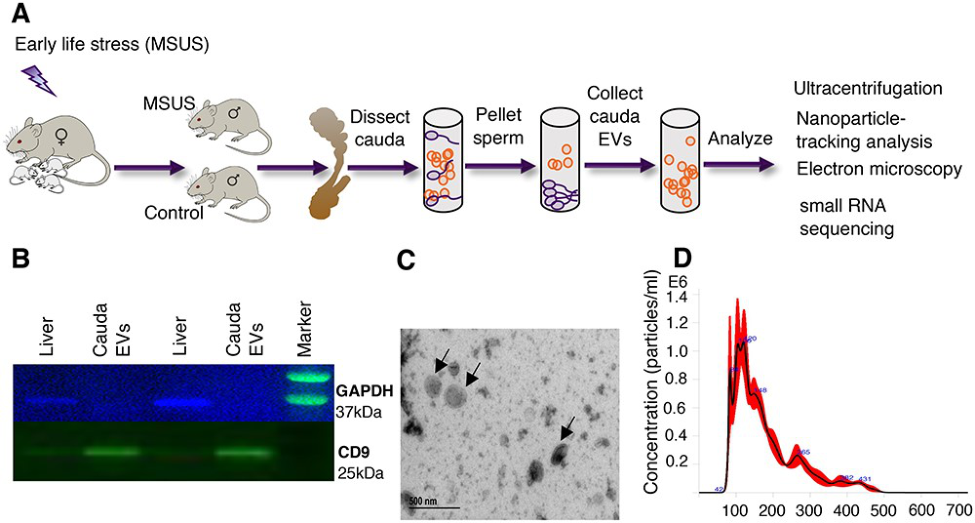
\includegraphics{thesis_files/figure-latex/ef1-1} 

}

\caption[Isolation and characterization of cauda epididymosomes]{\textbf{Isolation and characterization of cauda epididymosomes.} \newline \textbf{A:} Schematic representation of cauda epididymosomes preparation. \newline \textbf{B:} Immunoblot analysis was used to confirm the purity of isolation by staining with epididymosomal marker CD9 and absence of cellular marker GAPDH in the ultracentrifuged pellet. \newline \textbf{C:} Electron microscopy images of the preparations were used to assess the size and heterogeneity of the isolated populations. Arrows indicate cauda epididymosomes. \newline \textbf{D:} Nanoparticle-tracking analysis by dynamic light scattering showed particles of expected size of 50--300 nm.}\label{fig:ef1}
\end{figure}

\begin{figure}[htbp]

{\centering 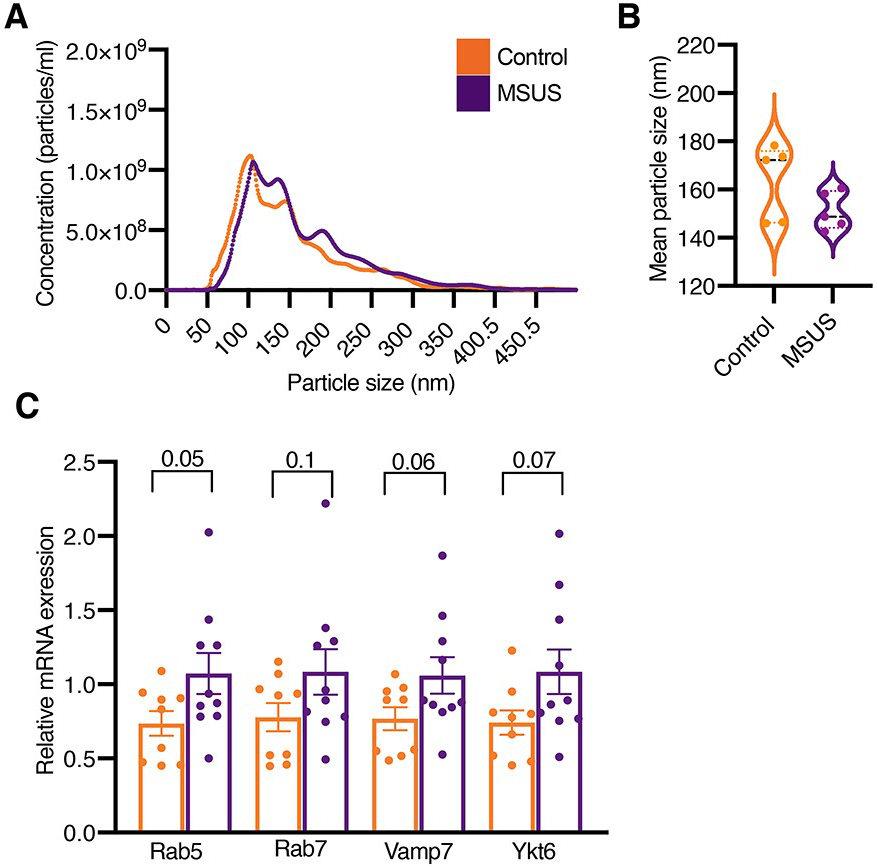
\includegraphics{thesis_files/figure-latex/ef2-1} 

}

\caption[Comparison of epididymosomal number, size, and release machinery in adult MSUS and control males]{\textbf{Comparison of epididymosomal number, size, and release machinery in adult MSUS and control males.} \newline \textbf{A:} Nanoparticle-tracking analysis showed no difference in the number of cauda epididymosomes between MSUS and control males. The plots were generated from average values across replicates (\emph{N} = 5 animals/group). Data are presented as mean ± standard error of the mean (SEM). \emph{P} \textless{} 0.05. \newline \textbf{B:} Quantification of nanoparticle-tracking analysis showed the mean size of cauda epididymosomes was not changed between the two groups (\emph{N} = 5 animals/group). Data are presented as mean ± SEM. \emph{P} \textless{} 0.05. \newline \textbf{C} Expression of genes involved in vesicular secretion in the caput epididymis from adult males measured by qRT-PCR. The experiments were performed in triplicates without pooling (\emph{N} = 8 animals/group). \newline Expression of GAPDH was used as endogenous control to normalize the expression level of the target genes. Data are presented as mean ± SEM. \emph{P} \textless{} 0.05.}\label{fig:ef2}
\end{figure}

\begin{figure}[htbp]

{\centering 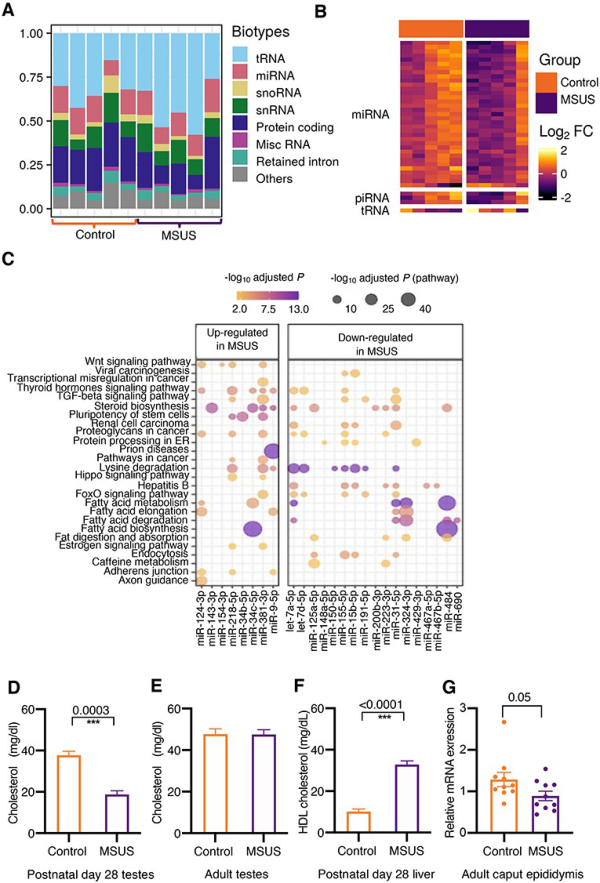
\includegraphics{thesis_files/figure-latex/ef3-1} 

}

\caption[Target pathways of up- and down-regulated miRNAs in adult MSUS cauda epididymosomes and alterations in steroidogenesis in postnatal and adult MSUS males]{\textbf{Target pathways of up- and down-regulated miRNAs in adult MSUS cauda epididymosomes and alterations in steroidogenesis in postnatal and adult MSUS males.} \newline \textbf{A:} Representative distribution of RNA biotypes from cauda epididymosomal sequencing (\emph{N} = 10 animals, 5 animals/group). \newline \textbf{B:} Heatmap of the most abundant small RNAs (\emph{n} = 39). Expression fold-change (log\textsubscript{2} FC) was calculated by subtracting log\textsubscript{2} counts per million of MSUS from controls. Each row depicts a small RNA and each column depicts a sample. Samples and RNAs are ordered by ``PCA'' method using \texttt{seriation} (R package). \newline \textbf{C:} Dot plot of miRNAs and pathways. Color-scale of the dot represents -log\textsubscript{10} adjusted \emph{P} of miRNA in a pathway and size of the dot represents --log\textsubscript{10} adjusted \emph{P} of the pathway. \newline Total cholesterol measurements in whole testes of males at postnatal day 28 (\emph{N} = 4 males/group) \textbf{D} and adulthood (\emph{N} = 10 controls, \emph{N} = 7 MSUS) \textbf{E}. \textbf{F:} HDL cholesterol level in the liver of males at postnatal day 28 (\emph{N} = 6 males/group). \newline \textbf{G:} Relative expression level of the androgen receptor in adult caput epididymis measured by qRT-PCR. qRT-PCR experiments were performed in triplicates, without pooling (\emph{N} = 10 animals/group). \newline \textbf{(D–G)} Data are presented as mean ± SEM. \emph{P} \textless{} 0.05.}\label{fig:ef3}
\end{figure}

\begin{figure}[htbp]

{\centering 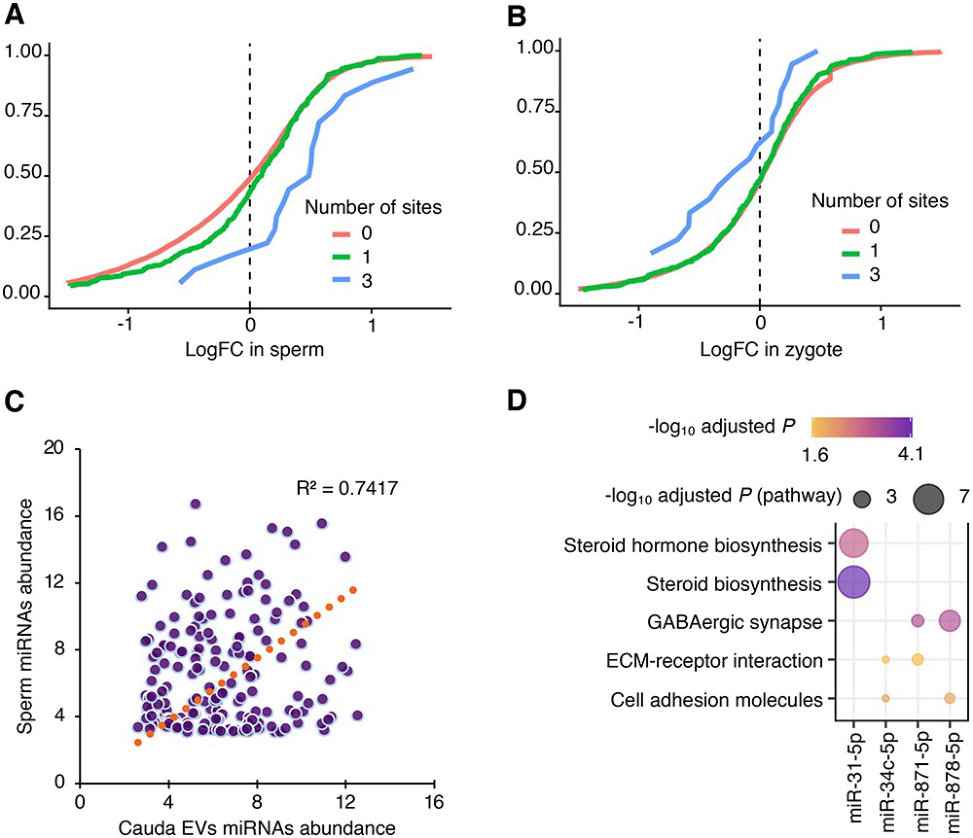
\includegraphics{thesis_files/figure-latex/ef4-1} 

}

\caption{\textbf{Targets of miRNAs from cauda epididymosomes are altered by MSUS in sperm and zygotes.} \newline Cumulative distribution plots of miR-31-5p targets from 5-months old MSUS and control caudal sperm RNA-seq \textbf{A} and from RNA-seq of zygotes originating from 3-months old MSUS and control males \textbf{B}. \newline \textbf{C:} miRNA abundance of sperm plotted against abundance in cauda epididymosomes. Coefficient of determination (\emph{R}\textsuperscript{2}=0.74). \newline \textbf{D:} Dot plot of the top target pathways (adjusted \emph{P} \textless{} 0.05) of miRNAs differentially expressed (adjusted \emph{P} \(\leq\) 0.1) in adult MSUS cauda epididymosomes. Color-scale of the dot represents --log\textsubscript{10} adjusted \emph{P} of miRNA in a pathway and size of the dot represents --log\textsubscript{10} adjusted \emph{P} of the pathway.}\label{fig:ef4}
\end{figure}
\hypertarget{supplementary-figures-1}{%
\section{Supplementary figures}\label{supplementary-figures-1}}


\begin{figure}[htbp]

{\centering 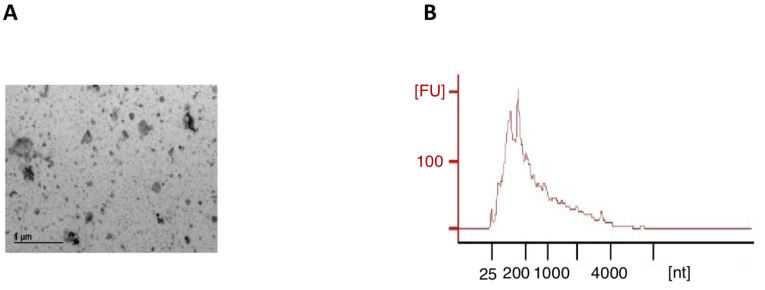
\includegraphics{thesis_files/figure-latex/es1-1} 

}

\caption[Electron microscopy image and electrophoresis]{\textbf{Electron microscopy image and electrophoresis.} \newline \textbf{A:} Electron microscopy image of the preparations were used to access the size and heterogeneity of the isolated populations. \newline \textbf{B:} The RNA amount of epididymosomes preparations was assessed by high-resolution automated electrophoresis.}\label{fig:es1}
\end{figure}

\begin{figure}[htbp]

{\centering 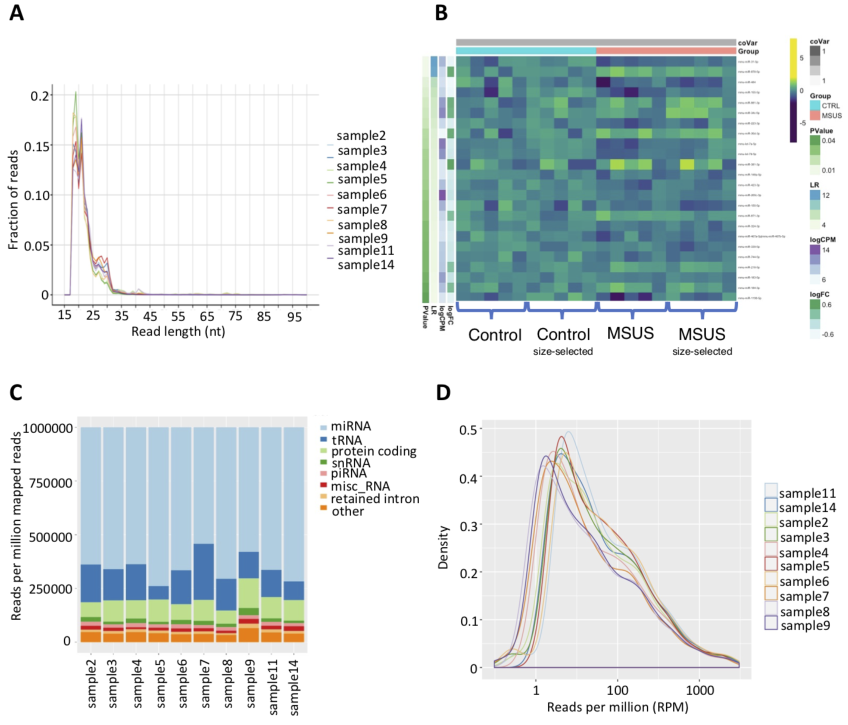
\includegraphics{thesis_files/figure-latex/es2-1} 

}

\caption[Data overview]{\textbf{Data overview.} \newline \textbf{A:} RNA read-length distributions of cauda epididymosomal small RNAs after size-selection. \newline \textbf{B:} Heatmap of top miRNAs of cauda epididymosomal small RNA-seq before and after size-selection. Each row depicts a miRNA and each column depicts a sample. (\emph{N} = 10 Controls, \emph{N} = 10 MSUS). \newline \textbf{C:} Representative distribution of RNA biotypes from cauda epididymosomal small RNA-seq after size-selection. (\emph{N} = 5 Controls, \emph{N} = 5 MSUS). \newline \textbf{D} miRNA abundance distributions plot of cauda epididymosomal small RNA-seq. (\emph{N} = 10 Controls, \emph{N} = 10 MSUS)}\label{fig:es2}
\end{figure}

\begin{figure}[htbp]

{\centering 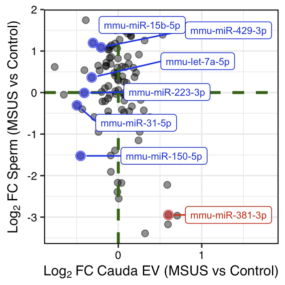
\includegraphics{thesis_files/figure-latex/es3-1} 

}

\caption[Scatterplot of log fold-change of miRNAs in sperm and cauda epididymosomes]{\textbf{Scatterplot of log fold-change of miRNAs in sperm and cauda epididymosomes.} miRNAs down-regulated (blue) and up-regulated (red) in MSUS cauda epididymosomes.}\label{fig:es3}
\end{figure}

\begin{figure}[htbp]

{\centering 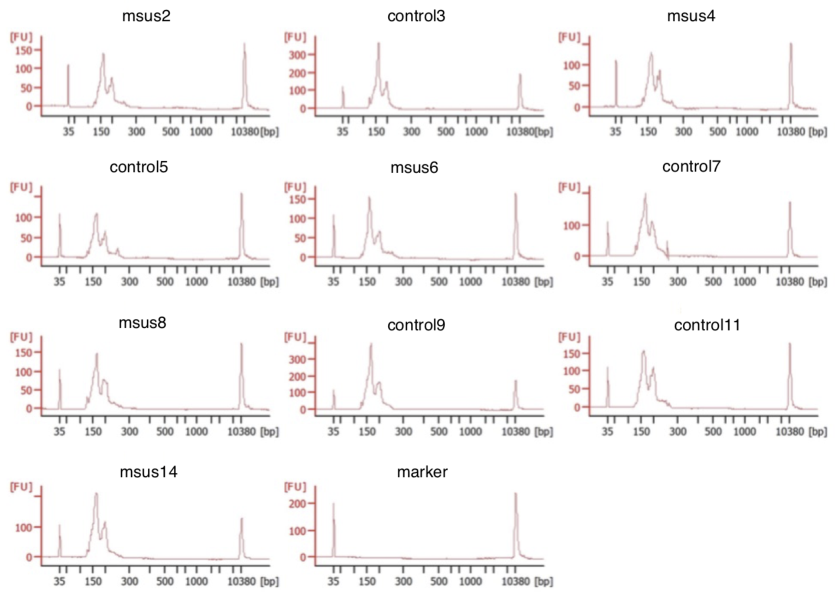
\includegraphics{thesis_files/figure-latex/es4-1} 

}

\caption[Profiles of cauda epididymosomal small RNAs by high-resolution automated electrophoresis]{\textbf{Profiles of cauda epididymosomal small RNAs by high-resolution automated electrophoresis.} (\emph{N} = 10 Controls, \emph{N} = 10 MSUS).}\label{fig:es4}
\end{figure}

\begin{figure}[htbp]

{\centering 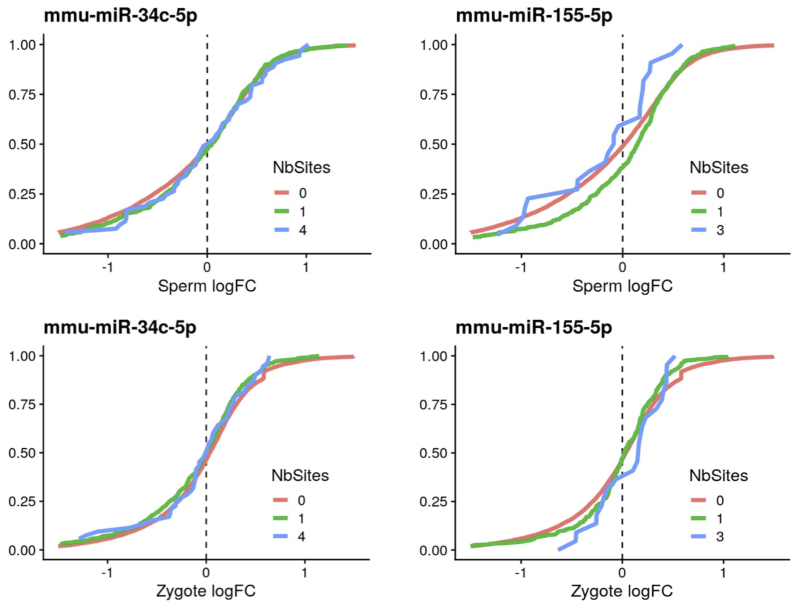
\includegraphics{thesis_files/figure-latex/es5-1} 

}

\caption[Cumulative distribution plots of miRNA targets in differentially expressed genes]{\textbf{Cumulative distribution plots of miR-34c-5p, miR-155-5p targets in differentially expressed genes (P $\le$ 0.05) from MSUS sperm and zygote RNA-sequencing.}}\label{fig:es5}
\end{figure}

\begin{figure}[htbp]

{\centering \includegraphics{thesis_files/figure-latex/es6-1} 

}

\caption[Immunoblot images of cauda epididymosomes and liver cell lysate, stained with cellular marker GAPDH (37kDa) and extracellular vesicle marker CD9 (25kDa)]{\textbf{Immunoblot images of cauda epididymosomes and liver cell lysate, stained with cellular marker GAPDH (37kDa) and extracellular vesicle marker CD9 (25kDa).} Same membrane was incubated and imaged separately.}\label{fig:es6}
\end{figure}
\hypertarget{supplementary-tables}{%
\section{Supplementary Tables}\label{supplementary-tables}}
\begin{table}[H]

\caption{\label{tab:est1}Supplementary table 1}
\centering
\resizebox{\linewidth}{!}{
\begin{tabular}[t]{lrrrrr}
\toprule
microRNA & logFC & logCPM & LR & PValue & FDR\\
\midrule
\cellcolor{gray!6}{mmu-miR-871-3p} & \cellcolor{gray!6}{0.4224445} & \cellcolor{gray!6}{7.865090} & \cellcolor{gray!6}{11.917353} & \cellcolor{gray!6}{0.0005560} & \cellcolor{gray!6}{0.0721259}\\
mmu-miR-31-5p & -0.3876365 & 9.998799 & 11.067851 & 0.0008780 & 0.0721259\\
\cellcolor{gray!6}{mmu-miR-155-5p} & \cellcolor{gray!6}{-0.4509784} & \cellcolor{gray!6}{7.903016} & \cellcolor{gray!6}{10.270414} & \cellcolor{gray!6}{0.0013518} & \cellcolor{gray!6}{0.0721259}\\
mmu-miR-881-3p & 0.2898815 & 11.465624 & 9.947026 & 0.0016111 & 0.0721259\\
\cellcolor{gray!6}{mmu-miR-878-5p} & \cellcolor{gray!6}{0.4517734} & \cellcolor{gray!6}{7.616360} & \cellcolor{gray!6}{9.829572} & \cellcolor{gray!6}{0.0017173} & \cellcolor{gray!6}{0.0721259}\\
\addlinespace
mmu-let-7f-5p & -0.2539420 & 15.094684 & 8.265118 & 0.0040414 & 0.1414491\\
\cellcolor{gray!6}{mmu-let-7a-5p} & \cellcolor{gray!6}{-0.3252566} & \cellcolor{gray!6}{13.378699} & \cellcolor{gray!6}{7.854573} & \cellcolor{gray!6}{0.0050692} & \cellcolor{gray!6}{0.1507945}\\
mmu-miR-34c-5p & 0.3699764 & 12.490816 & 7.628736 & 0.0057446 & 0.1507945\\
\cellcolor{gray!6}{mmu-let-7c-5p} & \cellcolor{gray!6}{-0.2660684} & \cellcolor{gray!6}{14.170724} & \cellcolor{gray!6}{6.590841} & \cellcolor{gray!6}{0.0102505} & \cellcolor{gray!6}{0.2391777}\\
mmu-let-7d-5p & -0.2957245 & 12.060525 & 6.254407 & 0.0123885 & 0.2514734\\
\addlinespace
\cellcolor{gray!6}{mmu-miR-148a-5p} & \cellcolor{gray!6}{-0.3860498} & \cellcolor{gray!6}{6.582776} & \cellcolor{gray!6}{6.099744} & \cellcolor{gray!6}{0.0135201} & \cellcolor{gray!6}{0.2514734}\\
mmu-miR-486a-5p|mmu-miR-486b-5p & 0.4242328 & 9.175211 & 5.992121 & 0.0143699 & 0.2514734\\
\cellcolor{gray!6}{mmu-miR-223-3p} & \cellcolor{gray!6}{-0.3918551} & \cellcolor{gray!6}{7.627599} & \cellcolor{gray!6}{5.758552} & \cellcolor{gray!6}{0.0164086} & \cellcolor{gray!6}{0.2650618}\\
mmu-miR-142a-5p & -0.3388176 & 7.860399 & 5.331804 & 0.0209397 & 0.2995186\\
\cellcolor{gray!6}{mmu-miR-484} & \cellcolor{gray!6}{-0.4464519} & \cellcolor{gray!6}{7.035887} & \cellcolor{gray!6}{5.294393} & \cellcolor{gray!6}{0.0213942} & \cellcolor{gray!6}{0.2995186}\\
\addlinespace
mmu-miR-182-5p & -0.1858805 & 11.537582 & 5.084665 & 0.0241383 & 0.3168156\\
\cellcolor{gray!6}{mmu-miR-183-5p} & \cellcolor{gray!6}{-0.2106265} & \cellcolor{gray!6}{11.356649} & \cellcolor{gray!6}{4.759219} & \cellcolor{gray!6}{0.0291418} & \cellcolor{gray!6}{0.3395679}\\
mmu-let-7g-5p & -0.1769275 & 14.499171 & 4.704360 & 0.0300862 & 0.3395679\\
\cellcolor{gray!6}{mmu-miR-181d-5p} & \cellcolor{gray!6}{0.2729988} & \cellcolor{gray!6}{7.492399} & \cellcolor{gray!6}{4.642132} & \cellcolor{gray!6}{0.0311962} & \cellcolor{gray!6}{0.3395679}\\
mmu-miR-467a-5p|mmu-miR-467b-5p & -0.3391907 & 6.822511 & 4.509472 & 0.0337076 & 0.3395679\\
\bottomrule
\end{tabular}}
\end{table}
\begin{table}[H]

\caption{\label{tab:est2}Supplementary table 2}
\centering
\resizebox{\linewidth}{!}{
\begin{tabular}[t]{lrrlrrrlr}
\toprule
Glul & logFC 1.00 & meanExpr
7.7 & PValue
2.4e-06 & FDR 0.0042 & sites
2 & targetscan .score
-0.60 & ...8 & conserved.sites
1\\
\midrule
\cellcolor{gray!6}{Pik3c2a} & \cellcolor{gray!6}{1.00} & \cellcolor{gray!6}{4.2} & \cellcolor{gray!6}{3.0e-06} & \cellcolor{gray!6}{0.0048} & \cellcolor{gray!6}{2} & \cellcolor{gray!6}{-0.36} & \cellcolor{gray!6}{NA} & \cellcolor{gray!6}{2}\\
Trankl & 0.93 & 4.7 & 6.9e-05 & 0.0240 & 3 & -0.53 & NA & 1\\
\cellcolor{gray!6}{Wdr5} & \cellcolor{gray!6}{1.00} & \cellcolor{gray!6}{1.8} & \cellcolor{gray!6}{2.le-03} & \cellcolor{gray!6}{0.1000} & \cellcolor{gray!6}{2} & \cellcolor{gray!6}{-0.65} & \cellcolor{gray!6}{NA} & \cellcolor{gray!6}{1}\\
Eif5 & 0.93 & 5.2 & 8.4e-05 & 0.0260 & 1 & -0.39 & NA & 1\\
\cellcolor{gray!6}{Bicdl} & \cellcolor{gray!6}{1.10} & \cellcolor{gray!6}{3.7} & \cellcolor{gray!6}{1.le-04} & \cellcolor{gray!6}{0.0280} & \cellcolor{gray!6}{2} & \cellcolor{gray!6}{-0.23} & \cellcolor{gray!6}{NA} & \cellcolor{gray!6}{1}\\
\bottomrule
\end{tabular}}
\end{table}
\begin{table}[H]

\caption{\label{tab:est3}Supplementary table 3}
\centering
\resizebox{\linewidth}{!}{
\begin{tabular}[t]{lrrrrrrlr}
\toprule
Hsf2bp & logFC
-2.30 & meanExpr
-1.60 & PValue 0.0300 & FDR 0.12 & sites
1 & targetscan .score
-0.460 & ...8 & conserved.sites
1\\
\midrule
\cellcolor{gray!6}{Satb2} & \cellcolor{gray!6}{-1.90} & \cellcolor{gray!6}{-1.60} & \cellcolor{gray!6}{0.0110} & \cellcolor{gray!6}{0.12} & \cellcolor{gray!6}{2} & \cellcolor{gray!6}{-0.380} & \cellcolor{gray!6}{NA} & \cellcolor{gray!6}{2}\\
Dpep3 & -2.50 & -2.90 & 0.0029 & 0.12 & 1 & -0.019 & NA & 1\\
\cellcolor{gray!6}{Jazf1} & \cellcolor{gray!6}{-1.20} & \cellcolor{gray!6}{-0.23} & \cellcolor{gray!6}{0.0015} & \cellcolor{gray!6}{0.12} & \cellcolor{gray!6}{2} & \cellcolor{gray!6}{-0.640} & \cellcolor{gray!6}{NA} & \cellcolor{gray!6}{1}\\
Ret & -1.90 & -1.80 & 0.0100 & 0.12 & 2 & -0.250 & NA & 1\\
\cellcolor{gray!6}{Wdr5} & \cellcolor{gray!6}{-0.93} & \cellcolor{gray!6}{2.50} & \cellcolor{gray!6}{0.0360} & \cellcolor{gray!6}{0.12} & \cellcolor{gray!6}{2} & \cellcolor{gray!6}{-0.650} & \cellcolor{gray!6}{NA} & \cellcolor{gray!6}{1}\\
\addlinespace
Snx22 & -1.70 & -1.30 & 0.0067 & 0.12 & 2 & -0.250 & NA & 2\\
\cellcolor{gray!6}{Rab9b} & \cellcolor{gray!6}{-1.20} & \cellcolor{gray!6}{-4.30} & \cellcolor{gray!6}{0.0380} & \cellcolor{gray!6}{0.12} & \cellcolor{gray!6}{2} & \cellcolor{gray!6}{-0.490} & \cellcolor{gray!6}{NA} & \cellcolor{gray!6}{1}\\
Nr5a2 & -1.50 & 1.30 & 0.0140 & 0.12 & 1 & -0.320 & NA & 1\\
\cellcolor{gray!6}{Plinl} & \cellcolor{gray!6}{-2.70} & \cellcolor{gray!6}{-0.62} & \cellcolor{gray!6}{0.0290} & \cellcolor{gray!6}{0.12} & \cellcolor{gray!6}{1} & \cellcolor{gray!6}{-0.210} & \cellcolor{gray!6}{NA} & \cellcolor{gray!6}{0}\\
\bottomrule
\end{tabular}}
\end{table}
\begin{table}[H]

\caption{\label{tab:est4}Supplementary table 4}
\centering
\resizebox{\linewidth}{!}{
\begin{tabular}[t]{lrrrrr}
\toprule
RNA & logFC & logCPM & LR & PValue & FDR\\
\midrule
\cellcolor{gray!6}{Prr15:protein\_coding} & \cellcolor{gray!6}{-0.7873999} & \cellcolor{gray!6}{4.547372} & \cellcolor{gray!6}{30.18055} & \cellcolor{gray!6}{0.0000000} & \cellcolor{gray!6}{0.0001084}\\
Gm15806:processed\_pseudogene & -0.6498672 & 6.510597 & 25.26703 & 0.0000005 & 0.0006874\\
\cellcolor{gray!6}{mmu-miR-34c-5p} & \cellcolor{gray!6}{0.7802879} & \cellcolor{gray!6}{11.007007} & \cellcolor{gray!6}{17.68464} & \cellcolor{gray!6}{0.0000261} & \cellcolor{gray!6}{0.0184327}\\
mmu\_piR\_004086 & 0.9769300 & 6.282539 & 17.63425 & 0.0000268 & 0.0184327\\
\cellcolor{gray!6}{Gm42427:TEC} & \cellcolor{gray!6}{-0.6134632} & \cellcolor{gray!6}{8.603910} & \cellcolor{gray!6}{16.67736} & \cellcolor{gray!6}{0.0000443} & \cellcolor{gray!6}{0.0244041}\\
\addlinespace
Gata3:protein\_coding & -0.4928509 & 6.189582 & 16.11356 & 0.0000597 & 0.0273818\\
\cellcolor{gray!6}{mmu-miR-878-5p} & \cellcolor{gray!6}{0.8891784} & \cellcolor{gray!6}{6.148635} & \cellcolor{gray!6}{15.77038} & \cellcolor{gray!6}{0.0000715} & \cellcolor{gray!6}{0.0281354}\\
Hpgd:protein\_coding & -0.5320409 & 8.066485 & 15.16616 & 0.0000985 & 0.0338922\\
\cellcolor{gray!6}{Ccdc136:protein\_coding} & \cellcolor{gray!6}{0.6987606} & \cellcolor{gray!6}{4.387168} & \cellcolor{gray!6}{14.00494} & \cellcolor{gray!6}{0.0001823} & \cellcolor{gray!6}{0.0472578}\\
mmu-miR-181d-5p & 0.6157888 & 5.694342 & 13.85633 & 0.0001973 & 0.0472578\\
\addlinespace
\cellcolor{gray!6}{Tacc2:protein\_coding} & \cellcolor{gray!6}{-0.5657623} & \cellcolor{gray!6}{4.398129} & \cellcolor{gray!6}{13.69020} & \cellcolor{gray!6}{0.0002156} & \cellcolor{gray!6}{0.0472578}\\
mmu-miR-871-3p & 0.6763168 & 6.446751 & 13.66182 & 0.0002189 & 0.0472578\\
\cellcolor{gray!6}{mmu-miR-9-5p} & \cellcolor{gray!6}{0.7204504} & \cellcolor{gray!6}{6.140215} & \cellcolor{gray!6}{13.49688} & \cellcolor{gray!6}{0.0002390} & \cellcolor{gray!6}{0.0472578}\\
Gm26168:misc\_RNA & 0.6325019 & 4.872739 & 13.22844 & 0.0002757 & 0.0472578\\
\cellcolor{gray!6}{Gm23921:misc\_RNA} & \cellcolor{gray!6}{0.5727151} & \cellcolor{gray!6}{6.650877} & \cellcolor{gray!6}{13.21883} & \cellcolor{gray!6}{0.0002772} & \cellcolor{gray!6}{0.0472578}\\
\addlinespace
Abcg2:nonsense\_mediated\_decay & -0.5214647 & 6.638810 & 13.19591 & 0.0002806 & 0.0472578\\
\cellcolor{gray!6}{Hipk3:protein\_coding} & \cellcolor{gray!6}{-0.4861401} & \cellcolor{gray!6}{4.791792} & \cellcolor{gray!6}{12.68259} & \cellcolor{gray!6}{0.0003691} & \cellcolor{gray!6}{0.0472578}\\
Odf1:protein\_coding & 0.5552237 & 6.042366 & 12.63222 & 0.0003792 & 0.0472578\\
\cellcolor{gray!6}{mmu-miR-881-3p} & \cellcolor{gray!6}{0.8813852} & \cellcolor{gray!6}{10.064670} & \cellcolor{gray!6}{12.60867} & \cellcolor{gray!6}{0.0003840} & \cellcolor{gray!6}{0.0472578}\\
mmu-miR-455-5p & 0.6872305 & 5.255313 & 12.60016 & 0.0003857 & 0.0472578\\
\addlinespace
\cellcolor{gray!6}{Snord88a:snoRNA} & \cellcolor{gray!6}{0.6180176} & \cellcolor{gray!6}{5.030322} & \cellcolor{gray!6}{12.50995} & \cellcolor{gray!6}{0.0004048} & \cellcolor{gray!6}{0.0472578}\\
His & 1.1442782 & 10.636565 & 12.47395 & 0.0004127 & 0.0472578\\
\cellcolor{gray!6}{Rnf2:protein\_coding} & \cellcolor{gray!6}{-0.4823013} & \cellcolor{gray!6}{4.596362} & \cellcolor{gray!6}{12.32996} & \cellcolor{gray!6}{0.0004457} & \cellcolor{gray!6}{0.0472578}\\
Gm10524:TEC & -0.4943310 & 5.296549 & 12.29409 & 0.0004544 & 0.0472578\\
\cellcolor{gray!6}{Ptgr1:protein\_coding} & \cellcolor{gray!6}{-0.4927718} & \cellcolor{gray!6}{6.068551} & \cellcolor{gray!6}{12.28196} & \cellcolor{gray!6}{0.0004574} & \cellcolor{gray!6}{0.0472578}\\
\addlinespace
Abcg2:protein\_coding & -0.5283684 & 7.721448 & 12.26538 & 0.0004614 & 0.0472578\\
\cellcolor{gray!6}{mmu-miR-218-5p} & \cellcolor{gray!6}{0.6591410} & \cellcolor{gray!6}{7.439262} & \cellcolor{gray!6}{12.23378} & \cellcolor{gray!6}{0.0004693} & \cellcolor{gray!6}{0.0472578}\\
iMet & 0.8698821 & 9.497592 & 12.18997 & 0.0004805 & 0.0472578\\
\bottomrule
\end{tabular}}
\end{table}
\hypertarget{chapter3}{%
\chapter{shortRNA}\label{chapter3}}

\begingroup\LARGE

\texttt{shortRNA}: a flexible framework for the analysis of short RNA sequencing data\newline
\begingroup\Large
\normalsize

\textbf{Contributions:} \emph{I worked towards the tool development, data analysis, results interpretation. This has been done together with Pierre-Luc Germain.}

\hypertarget{abstract-2}{%
\section{Abstract}\label{abstract-2}}

Short RNA are important molecules that play key functional roles in the
regulation of the genome. Several classes of short RNAs, such as miRNA,
tRNA and tRNA fragments, and piRNAs have been characterized and have
complex biogenesis. Short RNA sequencing is becoming increasingly
relevant in the research of regulatory mechanisms in a wide range of
biological functions. From an analysis point of view, each type of RNA
has its own features, and hence, specialized methods have been developed
focused on particular types, which not only multiply the work needed for
a comprehensive analysis but potentially create misassignment problems.
In addition, methods are typically divided into genome-based methods
that do not deal adequately with post-transcriptional modifications, and
transcript-based methods that are blind to unannotated features.
Finally, there are several outstanding issues in the analysis of short
RNAs, which are critical in the analysis of some samples. There is,
therefore, a need for an analysis framework that is: sufficiently
tailored to consider the specificities of different classes of short RNA
and their biogenesis, and sufficiently general and exhaustive to perform
global analyses. We developed a user-friendly, highly flexible and
comprehensive \texttt{R} package for a thorough end-to-end analysis of short RNA
sequencing data (planned submission to Bioconductor). Our package is
appropriately adapted to take into account the differences between
different types of short RNA and their biogenesis and is seamlessly
expandable to include additional annotation. We use a customized genome
annotation with artificial chromosomes to account for
post-transcriptional modifications, and a flexible rule-based approach
to assign reads along a tree of hierarchically organized features. This
enables the systematic querying, exploration, and differential
expression analysis of short RNAs at various degrees of granularity,
from specific sequences to RNA classes. We also include various
normalization and experimental-bias correction methods.The \texttt{shortRNA} \texttt{R} package is developed to perform all the steps from within \texttt{R} and is
platform-independent.

\hypertarget{introduction-and-background}{%
\section{Introduction and background}\label{introduction-and-background}}

Previous decades have revealed a number of RNAs that are distinct from
the messenger RNAs. Short-RNAs are non-coding RNA molecules that are
fewer than 200 nucleotides long and play an important role in genome
regulation. Several types of short RNAs, of different lengths, have been
discovered including microRNA (miRNA; 18-24 nt); small interfering RNA
(siRNA; 21-27 nt); small nucleolar RNA (snoRNA; 60-170 nt); small
nuclear RNA (snRNA/ U-RNA; 10-300 nt); Small temporal RNA (stRNA; 18-24
nt); tRNA-derived small RNA (tsRNA), including tRNA halves (tsRNA; 28-36
nt) and tRNA fragments (tRFs; 14-22 nt); small rDNA-derived RNA (srRNA;
18-30 nt); repeat-associated small interfering RNA (rasiRNA; 24-27 nt);
and Piwi-interacting RNA {[}piRNA; 26-31 nt, present in animals in the
germline cells and also in the brain (\protect\hyperlink{ref-zuo2016}{Zuo, Wang, Tan, Chen, \& Luo, 2016}). Some short RNAs, for
instance, miRNA and siRNA, are known to suppress gene expression by
sequence-specific interactions with regulatory regions during
transcription, RNA processing and translation (\protect\hyperlink{ref-zhu2016}{J. Zhu et al., 2016}), and by forming
the core with RNA-induced silencing complex (RISC) (\protect\hyperlink{ref-pratt2009}{Pratt \& MacRae, 2009}). In
addition, short-RNAs have been related to cancer, Parkinson's disease,
Alzheimer's disease, and prion disease (\protect\hyperlink{ref-gong2005}{Gong, Liu, Liu, \& Liang, 2005}), and hence, are used
as biomarkers.

Several methods have been developed for the analyses of short RNA
sequencing data. The development of high-throughput sequencing (HTS)
techniques allows researchers to study short RNAs in diverse tissues or
cells. HTS not only allows for the quantification of known short RNAs
but also for the identification and quantification of novel short RNAs.
The small RNA sequencing (sRNA-Seq) bears challenges and biases that
researchers need to be informed of in order to properly analyze the
data. First, most of the methods concentrate on a specific type of short
RNA, such as \texttt{MINTmap} (\protect\hyperlink{ref-loher2017}{Loher, Telonis, \& Rigoutsos, 2017}) focus on analyzing tRFs, \texttt{TAM\ 2.0}
(\protect\hyperlink{ref-li2018}{J. Li et al., 2018}), \texttt{Prost!} (\protect\hyperlink{ref-desvignes2019}{Desvignes, Batzel, Sydes, Eames, \& Postlethwait, 2019}), \texttt{Chimira} (\protect\hyperlink{ref-vitsios2015}{Vitsios \& Enright, 2015}), and \texttt{mirTools}
2.0 (\protect\hyperlink{ref-wu2013}{J. Wu et al., 2013}) focus on miRNAs. Next, a few tools concentrate on most
types of short RNAs (not all), such as \texttt{ncPRO-seq} (\protect\hyperlink{ref-chen2012}{C.-J. Chen et al., 2012}),
\texttt{sRNAtoolbox} (\protect\hyperlink{ref-rueda2015}{Rueda et al., 2015}), \texttt{SPAR} (\protect\hyperlink{ref-kuksa2018}{Kuksa et al., 2018}), \texttt{Threshold-seq} (\protect\hyperlink{ref-magee2017}{Magee, Loher, Londin, \& Rigoutsos, 2017}),
\texttt{sRNAnalyzer} (\protect\hyperlink{ref-wu2017}{Xiaogang Wu et al., 2017}), \texttt{UEA\ sRNA\ Workbench} (\protect\hyperlink{ref-stocks2012}{Stocks et al., 2012}), \texttt{Sports1}
(\protect\hyperlink{ref-shi2018}{Shi, Ko, Sanders, Chen, \& Zhou, 2018}), and \texttt{Oasis2} (\protect\hyperlink{ref-rahman2018}{Rahman et al., 2018}). Tools that concentrate on many
types of short RNAs, such as \texttt{Oasis2} and \texttt{Sports1}, perform sequential
mapping, for example, they perform sequential mapping by first assigning
the reads to miRNAs, then assigning the leftover to tRNAs, and then the
remaining ones to mRNAs, which can create a misassignment problem as
short reads can map to multiple locations. But this information is lost
because only unmapped reads are aligned against the next annotation. In
addition, althoughthe libraries for sequencing are tailored to short
RNAs, other long RNAs are also often detected in the sequencing data,
and also because short RNAs often overlap with other features,
prioritization between the biotypes is crucial. Further, there are quite
a high number of sequenced reads left that map to the reference genome
but are not assigned to the known features. Moreover, although most of
the tools do not consider assignment rules for reads assignment, few
tools such as Prost! have a set of defined rules for reads assignment.
But, the rules are only for the miRNAs. Furthermore, the multi-mapping
reads are either excluded or randomly assigned to the multi-mapping
positions in the genome. As well as, not all the tools deal with the
post-transcriptional modifications, such as the addition of ``CCA''
towards the 3' end of tRNAs (\protect\hyperlink{ref-barraud2019}{Barraud \& Tisné, 2019}; \protect\hyperlink{ref-hou2010}{Hou, 2010}; \protect\hyperlink{ref-ibba2000}{Ibba \& Soll, 2000}), which
is important for the recognition of tRNA by enzymes and translation
(\protect\hyperlink{ref-green1997}{R. Green \& Noller, 1997}; \protect\hyperlink{ref-sprinzl1979}{Sprinzl \& Cramer, 1979}); and the addition of ``G'' towards the 5' end
in histidine tRNAs (\protect\hyperlink{ref-cooley1982}{Cooley et al., 1982}; \protect\hyperlink{ref-cozen2015}{Cozen et al., 2015}), this is critical for
histidyl-tRNA synthetase (HisRS) recognition (\protect\hyperlink{ref-fromant2000}{Fromant, Plateau, \& Blanquet, 2000}), which is
responsible for the integration of histidine into proteins
(\protect\hyperlink{ref-freist1999}{Freist, Verhey, Rühlmann, Gauss, \& Arnez, 1999}). On top of these limitations, most of the tools are
written in different programming languages, are platform-dependent and
depend on external tools, which can create a barrier for installation
for the user; and the tools are either web-based, which restrict the
user for additional downstream analysis or command-line based, which
creates a restriction for the non-computational researchers. Besides,
the available tools use feature-based counting (number of reads, counts,
associated with each feature), except for \texttt{seqpac} (\protect\hyperlink{ref-skog2021}{Skog et al., 2021}), a recently
published tool, which uses sequence-based counting (number of reads,
counts, associated with each unique sequence). Sequence-based counting
would prevent the same sequence from being annotated multiple times
within and across samples, hence increasing the efficiency for alignment
and reads assignment. Also, it directly enables looking at specific
variations in sequences or their boundaries. However, due to this
complexity, it can be challenging to explore data at the level of
individual sequences, which calls for methods that can afford different
levels of granularity. Hence, specialized tools are required with
specialized pipelines to analyze sRNA-seq data.

We developed \texttt{shortRNA}, an R tool that addresses all of the issues listed
above for processing sRNA-seq data. Our tool is cross-platform (it may
run on any operating system) and built on the Bioconductor framework, in
particular making use of efficient data structures (e.g., \texttt{DataFrame},
\texttt{FactorList}, and \texttt{TreeSummarizedExperiment}) enabling interoperability with
other Bioconducto\texttt{R} packages. Users can use \texttt{shortRNA} to conduct a
thorough analysis of their data, from quality control (trimming, adapter
removal, UMI compressing) and alignment to quantification and downstream
analysis. \texttt{shortRNA} also has a set of customizable criteria for assigning
reads to various types of short RNAs and seamlessly enables querying
features at the level of individual fragments. We have tested our tool
using a published mouse dataset from sperm, simulated data from sperm,
and human data from peripheral blood mononuclear cells (PBMC;
unpublished).

\hypertarget{methods-2}{%
\section{Methods}\label{methods-2}}

\hypertarget{development-and-testing-environment}{%
\subsection{Development and testing environment}\label{development-and-testing-environment}}

The \texttt{shortRNA} package is developed and tested on the Linux (GNU/Linux
4.4.0-210-generic x86\_64) operating system, Ubuntu (version 16.04.7 LTS)
with 16 processors and 124 GB of RAM, using R 3.6.3 and R 4.0.5. As the
\texttt{shortRNA} tool is developed as an \texttt{R} package, it is platform-independent
(can easily be installed and run on other operating systems).

\hypertarget{backbone-data-structures-of-shortrna}{%
\subsection{\texorpdfstring{Backbone data structures of \texttt{shortRNA}}{Backbone data structures of shortRNA}}\label{backbone-data-structures-of-shortrna}}

The \texttt{shortRNA} package is developed around four main data structures from
Bioconductor: phylo, \texttt{FactorList}, \texttt{DataFrame}, and
\texttt{TreeSummarizedExperiment}. These four data structures store the data and
results in the most efficient manner and enable fast computation.

\hypertarget{phylo}{%
\subsubsection{phylo}\label{phylo}}

The phylogenetic tree is a branching diagram used to depict evolutionary
relationships. In R, the phylo class stores the phylogenetic
relationship. In \texttt{shortRNA}, we save the relationship between RNA
biotypes, features, and reads as a phylo object, section \protect\hyperlink{ft}{Features Tree}.

\hypertarget{factorlist}{%
\subsubsection{\texorpdfstring{\texttt{FactorList}}{FactorList}}\label{factorlist}}

In the case of a long vector of repeated characters, R takes more memory
to store them and also the computation could be quite slow. These
repeated character vectors could be stored as factors, where levels are
provided to each unique character in the vector
(\url{https://datascience.stackexchange.com/questions/12018/when-to-choose-character-instead-of-factor-in-r}).
However, when factors are stored in a list, the levels are traditionally
defined for each element of the list, which can be very inefficient
memory-wise. The \texttt{FactorList}, a class from the IRanges Bioconductor
package, instead stores lists of factors as a single factor vector with
added list membership information. In addition, like other AtomicList
objects, it enables list operations without iteration. This is helpful
for efficiently saving the object in R memory and for fast computations.

\hypertarget{dataframe}{%
\subsubsection{\texorpdfstring{\texttt{DataFrame}}{DataFrame}}\label{dataframe}}

Rectangular data can be stored as \texttt{data.frame} class object in R.
\texttt{DataFrame} functions from S4Vectors Bioconducto\texttt{R} package and behaves
similar to \texttt{data.frame} in terms of construction and subsetting. An
advantage of using \texttt{DataFrame} is that it can store any type of object in
a column, for example, a \texttt{FactorList}, or even another \texttt{DataFrame}, while
retaining all the methods and functionalities of traditional
\texttt{data.frame}s.

\hypertarget{treesummarizedexperiment}{%
\subsubsection{\texorpdfstring{\texttt{TreeSummarizedExperiment}}{TreeSummarizedExperiment}}\label{treesummarizedexperiment}}

\texttt{TreeSummarizedExperiment} is a Bioconducto\texttt{R} package extending the
classical \texttt{SummarizedExperiment} (\protect\hyperlink{ref-morgan2020}{Morgan, Obenchain, Hester, \& Pagès, 2020}) and with additional
hierarchy data and operations (\protect\hyperlink{ref-huang2020}{R. Huang et al., 2020}). The \texttt{SummarizedExperiment}
class holds rectangular matrices of experiment data, accompanied by row
and column annotation data. There are two classes in the
SummarizedExperiment package: \texttt{SummarizedExperiment} and
RangedSummarizedExperiment. Instead of a \texttt{DataFrame} of features,
RangedSummarizedExperiment objects represent genomic ranges of interest.
Figure \ref{fig:3f1}A depicts the structure of the \texttt{SummarizedExperiment}. The
rectangular data matrices are stored as assays, rowData stores
annotation for corresponding rows in the assays, colData stores
annotation for corresponding columns in the assays, ranges are described
by a GRanges or a GRangesList object, which are stored as rowRanges, and
metadata can be used to store additional data-related information.

In extension to the \texttt{SummarizedExperiment}, \texttt{TreeSummarizedExperiment} has
rowTree, which stores the hierarchical structure of rows of assays;
colTree, which stores hierarchical structure of columns of the assays;
rowLinks, which stores the link information between the rows of the
assays and rowTree; colLinks, which stores the link information between
the columns of the assays; and referenceSeq, which stores the reference
sequence for the features, depicted in Figure \ref{fig:3f1}B.


\begin{figure}[htbp]

{\centering \includegraphics{thesis_files/figure-latex/3f1-1} 

}

\caption{Schematic of A: \texttt{SummarizedExperiment} (\protect\hyperlink{ref-morgan2020}{Morgan et al., 2020}), B: \texttt{TreeSummarizedExperiment} (\protect\hyperlink{ref-huang2020}{R. Huang et al., 2020})}\label{fig:3f1}
\end{figure}
\hypertarget{pipeline}{%
\subsection{Pipeline}\label{pipeline}}

The \texttt{shortRNA} pipeline includes three major data analysis steps:
preprocessing of data, alignment and reads assignment with the
customisable assignment rules, and statistical analysis and
visualization. Figure \ref{fig:3f2} shows the outline of the pipeline. First, the
data goes through the preprocessing steps that consist of filtering and
alignment of unique sequenced reads. The raw data undergo quality
assessment and then the quality control steps are performed. The data is
then aligned to a custom genome containing, in addition to the reference
genome, extra pseudo-chromosomes for handling post-transcriptional
modifications. Aligned reads are then overlapped with the features
annotation and reads are assigned to the features using customisable
assignment rules, which is an important part of this pipeline, after
that, a features tree is formed. After the reads assignment, the data
goes through the statistical analysis steps that consist of
normalization and differential analysis. The quality controlled data are
normalized and then the test for differential expression of short RNAs
is performed in the user-defined biological groups.


\begin{figure}[htbp]

{\centering \includegraphics{thesis_files/figure-latex/3f2-1} 

}

\caption{Overview of \texttt{shortRNA} pipeline}\label{fig:3f2}
\end{figure}
\hypertarget{quality-control-and-trimming}{%
\subsubsection{Quality control and trimming}\label{quality-control-and-trimming}}

Quality control (QC) and trimming is a vital step in HTS data analysis.
To assess and control the quality of sRNA-Seq data, we adapted the
functionalities from two \texttt{R} packages: \texttt{Rfastp} (\protect\hyperlink{ref-wang2020}{W. Wang \& Carroll, 2020}) and seqTools
(\protect\hyperlink{ref-kaisers2020}{Kaisers, 2020}). \texttt{Rfastp} is used for trimming the low-quality reads and
adapter trimming. Further, with the summary files from \texttt{Rfastp}, the
functions in our tool could be used for making a table of comparison for
before and after QC, plots for duplicated reads, reads quality plot, and
base-content plots. We benchmarked Biostrings (\protect\hyperlink{ref-paguxe8s2020}{Pagès, Aboyoun, Gentleman, \& DebRoy, 2020}), qrqc
(\protect\hyperlink{ref-buffalo2020}{Buffalo, 2020}), ShortRead (\protect\hyperlink{ref-morgan2009}{Morgan et al., 2009}), and seqTools for reading and
storing FASTQ files quality data in \texttt{R}, using an 863 MB FASTQ file.
seqTools outperformed the other three tools in terms of reading and
storing the FASTQ file quality data, as shown in Figure \ref{fig:3f3}. Hence, we
used it for reading the FASTQ files quality data, before and after QC,
to make reads length distribution plots. To summarize, the QC functions
provide information about sequencing depth, reads quality, possible
adapter sequences, duplicated reads, and sequence length distribution,
both before and after QC. The interactive plots provide users with
greater insight into their data. Exemplary plots and tables from the QC
report of a sample are shown in Figure \ref{fig:3f4}.


\begin{figure}[htbp]

{\centering \includegraphics{thesis_files/figure-latex/3f3-1} 

}

\caption{Benchmark of four different Bioconductor tools for reading and storing FASTQ file quality data. Performance of four tools is measured in \textbf{A:} the amount of time they take for reading the file, \textbf{B:} the amount of memory they take to store the data.}\label{fig:3f3}
\end{figure}

\begin{figure}[htbp]

{\centering \includegraphics{thesis_files/figure-latex/3f4-1} 

}

\caption{Exemplary QC report plots of a sperm sample from (\protect\hyperlink{ref-gapp2021}{Katharina Gapp et al., 2021}). \textbf{A:} Quality control table, \textbf{B:} Quality score lines plot at each nucleotide in the sequencing reads, \textbf{C:} Barplot of reads duplication level with the mean GC ratio represented as lines, \textbf{D:} Histogram of reads distribution, before and after quality control}\label{fig:3f4}
\end{figure}
Unique Molecular Identifiers (UMIs) are complex indices of 8-16
nucleotide lengths that are introduced to sequencing libraries before
PCR amplification steps. Researchers can use UMI to evaluate the
efficiency with which they collect input molecules, identify sampling
bias, and, most importantly, identify and compensate for the effects of
PCR amplification bias (\protect\hyperlink{ref-fu2018}{Y. Fu, Wu, Beane, Zamore, \& Weng, 2018}). Preprocessing of data sequenced with
UMIs is required for reads deduplication and correction, as well as the
creation of consensus sequences from each UMI. In \texttt{shortRNA}, we have
adapted the \texttt{UMIc} tool for UMIs collapsing (\protect\hyperlink{ref-tsagiopoulou2021}{Tsagiopoulou et al., 2021}), which
takes into account the frequency and the Phred quality of nucleotides
and the distances between the UMIs and the actual sequences for
collapsing the sequences.

Schematic of quality checks and quality control is shown in Figure \ref{fig:3f5}.


\begin{figure}[htbp]

{\centering \includegraphics{thesis_files/figure-latex/3f5-1} 

}

\caption{Schematic of quality check and quality control of FASTQ files, UMIs collapsing (if present), and collapsing FASTQ files to obtain unique sequences for alignment and making a sequence by samples counts matrix}\label{fig:3f5}
\end{figure}
\hypertarget{sequence-count-matrix}{%
\subsubsection{Sequence count matrix}\label{sequence-count-matrix}}

From the trimmed FASTQ files, we extract the unique reads sequences and
make a sample by sequence count matrix. This matrix represents the
counts of sequences in each sample, keeping only sequences occurring
more than once. This is done by the \texttt{fastq2SeqCountMatrix()} function from
\texttt{shortRNA}. Further, we export these sequences as a fasta file. An
overview of this step is shown in Figure \ref{fig:3f5}. The two main outputs from
this step are sequenceFasta, which would be used for alignment, and
countsMatrix.

\hypertarget{annotation-preparation}{%
\subsubsection{Annotation preparation}\label{annotation-preparation}}

Sequencing generates nucleotide sequences with unknown functions, while
sequence annotation provides descriptive information about sequenced DNA
sequences. Several databases are available for the annotation of the
sequences. In \texttt{shortRNA}, we used miRBase (\protect\hyperlink{ref-griffiths-jones2008}{Griffiths-Jones, Saini, van Dongen, \& Enright, 2008}) for
miRNAs; GtRNADb (\protect\hyperlink{ref-chan2016}{P. P. Chan \& Lowe, 2016}) for tRNAs; mitoRNADb (\protect\hyperlink{ref-juxfchling2009}{Jühling et al., 2009}) for
mitochondrial tRNAs; for mouse, we use piRNA precursors from (\protect\hyperlink{ref-li2013}{X. Z. Li et al., 2013}),
rRNAs from SILVA (\protect\hyperlink{ref-quast2013}{Quast et al., 2013}), and mRNAs and other biotypes from Ensembl
(\protect\hyperlink{ref-howe2021}{Howe et al., 2021}). It is possible for users to have additional databases of
their choice.

The miRBase database is a collection of miRNA sequences and annotations.
In miRBase, miRNAs are named as, for example, org-mir-20a. The first 3
letters signify the organism, ``20'' tell us that it was an
early-discovered family (20th family that was named), ``20a'' tell us that
there is possibly another related miRNA, for example, org-mir-20a. Here,
org-mir-20a is a precursor. The mature miRNA species may be derived from
both the 5' and 3' arms of the precursor duplex, and are called the
miRNA-5p and -3p species, respectively. In this example, it would be
org-mir20a-5p and org-mir20a-3p. All the miRNAs overlapping between
Ensembl and miRBase were removed from Ensembl and the remaining one from
Ensembl, not overlapping, were renamed to match the nomenclature of
miRBase. For example, Mir7679 is renamed to org-miR-7679. Further, if
the length of Ensembl miRNAs were more than 25bp, we labelled them as
precursors.

A miRNA cluster is a group of two or more miRNA hairpins that are
transcribed from miRNA genes that are physically adjacent, transcribed
in the same direction, and are not separated by a transcription unit or
a miRNA in the opposite orientation. There are mostly 2-3 mature miRNAs
in a miRNA cluster, but there is an existence of a bigger miRNA cluster,
which is found in humans on chromosome 13: miR-17 to miR-92, involved in
tumour formation, and development of heart lungs and immune systems
(\protect\hyperlink{ref-lai2013}{Lai \& Vera, 2013}). Researchers group the miRNAs to form a miRNA cluster by the
distance between them. For example, (\protect\hyperlink{ref-baumgart2017}{Baumgart et al., 2017}; \protect\hyperlink{ref-griffiths-jones2008}{Griffiths-Jones et al., 2008}) call a group of miRNA as clusters if miRNAs are within
10kb and (\protect\hyperlink{ref-yuan2009}{Yuan et al., 2009}) used a distance of 50kb. In \texttt{shortRNA}, we use a
distance of 10kb for clustering miRNAs as more than 40\% of
experimentally validated human miRNA cluster genes have been identified
within 10kb (\protect\hyperlink{ref-griffiths-jones2008}{Griffiths-Jones et al., 2008}; \protect\hyperlink{ref-lai2013}{Lai \& Vera, 2013}).

The genomic tRNA database (GtRNADb) is a database of tRNA gene
predictions created by tRNAscan-SE (\protect\hyperlink{ref-chan2021}{P. Chan, Lin, Mak, \& Lowe, 2021}) on whole or almost
complete genomes. In GtRNADb, tRNAs symbols consist of 5 parts,
separated by a ``-'', for example, tRNA-Ala-AGC-9-2. In this example, tRNA
(prefix) represents tRNA genes that are high scoring and not predicted
as pseudogenes. If it was a pseudogene, it would have been represented
as ``tRX''. At the second position, we have three-letter amino acids
(isotype), which stand for tRNA isotype. At the third position, we have
anticodon detected in the gene sequence. At the fourth position, there
is a unique ID (transcript ID) of a tRNA transcript or ``isodecoder'' with
a particular isotype and anticodon. The fifth position represents the
gene locus ID and for tRNA genes with multiple identical copies, this
gene locus ID represents the particular gene copy in the genome. For the
mitochondrial tRNAs, we obtained the sequences from mitotRNAdb
(\protect\hyperlink{ref-juxfchling2009}{Jühling et al., 2009}) using the tRNAdbImport (\protect\hyperlink{ref-gm2018}{GM, 2018}) \texttt{R} package. Further, we
removed all the duplicated sequences and renamed the mitochondrial tRNAs
as per the naming convention of GtRNADb, adding ``mt'' as a prefix. Mature
tRNAs receive a post-transcriptional addition of ``CCA'' (\protect\hyperlink{ref-barraud2019}{Barraud \& Tisné, 2019}),
hence, we added ``CCA'' to all the tRNA/ mt-tRNA sequences at the 3' end.
All histidine tRNAs of known sequence are one nucleotide longer at the
5' end than are other tRNA species(\protect\hyperlink{ref-cozen2015}{Cozen et al., 2015}),hence we added ``G'' at the 5' end of the sequences of Histidine tRNAs/ mt-tRNAs to account for this post-translational modification, as also
done in (\protect\hyperlink{ref-cozen2015}{Cozen et al., 2015}; \protect\hyperlink{ref-shi2018}{Shi et al., 2018}). Because of these post-transcriptional
modifications, we add the sequences of tRNA into the genome FASTA file
as pseudo chromosomes. For example:
\begin{Shaded}
\begin{Highlighting}[]
\NormalTok{\textgreater{}pseudoChr\_tRNA{-}Thr{-}CGT{-}1{-}1}
\NormalTok{GGCGCGGTGGCCAAGTGGTAAGGCGTCGGTCTCGTAAACCGAAGATCACGGGTTCGAACCCCGTCCGTGCCTCCA}

\NormalTok{\textgreater{}pseudoChr\_mt\_tRNA{-}His{-}GTG{-}1{-}1}
\NormalTok{GGTGAATATAGTTTACAAAAAACATTAGACTGTGAATCTGACAACAGGAAATAAACCTCCTTGTTCACCCCA}
\end{Highlighting}
\end{Shaded}
All the tRNAs overlapping between Ensembl and GtRNADb were removed from
Ensembl and the remaining tRNA from Ensembl, not overlapping, were
labelled as pseudo tRNAs.

SILVA is an rRNA database, which provides extensive, quality-checked,
and regularly updated datasets of aligned short (16S/18S, SSU) and large
subunit (23S/28S, LSU) ribosomal RNA sequences. rRNAs are repeated
sequences and are masked in the genomes in the Ensembl database, and are
not listed in the features annotation. Hence, we add them as well as
pseudo chromosomes to the genome FASTA file, similar to tRNAs.

\texttt{getDB()}, Figure \ref{fig:3f6}, function retrieve the databases, account for the
post-translational modifications of tRNAs, alter mitochondrial tRNA
database, and create miRNA clusters and assign miRNAs and miRNA
precursors to miRNA clusters. The output from \texttt{getDB()} is then parsed to
the \texttt{prepareAnnotation()} function, which prepares features annotation as
\texttt{GRanges()}, save the genome and pseudo-genomes and index that for
alignment. Features annotation are then converted to \texttt{FactorList} using
\texttt{featuresAnnoToFL()}. The main three outputs from the annotation
preparation are features as \texttt{GRanges()} and \texttt{FactorList()}, and \texttt{indexed\ customGenome}.


\begin{figure}[htbp]

{\centering \includegraphics{thesis_files/figure-latex/3f6-1} 

}

\caption{Schematic of obtaining database, preparing annotations and custom genome indexes for alignment}\label{fig:3f6}
\end{figure}
\hypertarget{alignment}{%
\subsubsection{Alignment}\label{alignment}}

Alignment is necessary to know where in the genome reads belong. The
alignment of short RNA remains a persistent under-recognized problem. We
align the FASTA file of sequences with the custom genome prepared in the
annotation step. For alignment, we use the \texttt{Rsubread} \texttt{R} package
(\protect\hyperlink{ref-liao2019}{Liao et al., 2019}) with the index of custom genome generated on the genome and
pseudo-chromosomes (\texttt{index\ =\ "customGenome"}), with the GTF from Ensembl
database obtained from \texttt{getDB()} of \texttt{shortRNA} (\texttt{GTF\ =\ exonsBy(db\$ensdb)}),
and allowing to report the maximal number of equally-best mapping
locations (\texttt{nBestLocations\ =\ 16}). Please refer to the schematic in Figure
\ref{fig:3f7}.


\begin{figure}[htbp]

{\centering \includegraphics{thesis_files/figure-latex/3f7-1} 

}

\caption{Schematic of alignment, overlapping features and aligned sequences, and assigning reads to features using assignment rules}\label{fig:3f7}
\end{figure}
\hypertarget{reads-annotation-and-assignment}{%
\subsubsection{Reads annotation and assignment}\label{reads-annotation-and-assignment}}

After alignment, the aligned file (BAM file) is overlapped with the
features annotation (\texttt{featuresGR}) using the \texttt{overlapWithTx2()} function. It
is possible that a read overlaps with multiple features. Next, the
overlaps are parsed with the \texttt{assignReads()} function with the assignment
rules, \texttt{defaultAssignRules()}, for validating the overlap and finding
assignment of multi mapping reads. Please refer to the schematic in
Figure \ref{fig:3f7}.

\hypertarget{assignment-rules}{%
\subsubsection{Assignment rules}\label{assignment-rules}}

A sequence read can be mapped to multiple locations in the genome. It is
critical to ensure that the reads are properly mapped to the feature and
that they are assigned to one or more features. In the \texttt{shortRNA} package,
we defined a set of customizable rules for this purpose. The output of
the function \texttt{defaultAssignRules()} is described below:

We consider reads with at least 50\% overlap to the features to be valid
read assignments.
\begin{Shaded}
\begin{Highlighting}[]
\SpecialCharTok{$}\NormalTok{overlapBy}
\NormalTok{[}\DecValTok{1}\NormalTok{] }\FloatTok{0.5}
\end{Highlighting}
\end{Shaded}
By default, we do not prioritize the assignment based on the size of the
overlap between reads and features (when a read overlaps multiple
features); however this option is available to users.
\begin{Shaded}
\begin{Highlighting}[]
\SpecialCharTok{$}\NormalTok{prioritizeByOverlapSize}
\NormalTok{[}\DecValTok{1}\NormalTok{] }\ConstantTok{FALSE}
\end{Highlighting}
\end{Shaded}
We prioritize overlap in the same strand, but enable overlaps from the
opposite strand if there is no known feature on the same strand.
\begin{Shaded}
\begin{Highlighting}[]
\SpecialCharTok{$}\NormalTok{sameStrand}
\NormalTok{[}\DecValTok{1}\NormalTok{] }\StringTok{"prioritize"}
\end{Highlighting}
\end{Shaded}
We give priority to known features in our assignments.
\begin{Shaded}
\begin{Highlighting}[]
\SpecialCharTok{$}\NormalTok{prioritizeKnown}
\NormalTok{[}\DecValTok{1}\NormalTok{] }\ConstantTok{TRUE}
\end{Highlighting}
\end{Shaded}
Next come validation rules specific to RNA types. For example, in order
to be assigned to primary piRNAs, the read should be 26-32 nucleotides
long, with the first nucleotide being a T.
\begin{Shaded}
\begin{Highlighting}[]
\SpecialCharTok{$}\NormalTok{typeValidation}\SpecialCharTok{$}\NormalTok{primary\_piRNA}
\SpecialCharTok{$}\NormalTok{typeValidation}\SpecialCharTok{$}\NormalTok{primary\_piRNA}\SpecialCharTok{$}\NormalTok{fun}
\ControlFlowTok{function}\NormalTok{(src, }\AttributeTok{allowRevComp=}\ConstantTok{FALSE}\NormalTok{, }\AttributeTok{length=}\DecValTok{26}\SpecialCharTok{:}\DecValTok{32}\NormalTok{)\{}
\NormalTok{  length }\OtherTok{\textless{}{-}} \FunctionTok{as.integer}\NormalTok{(length)}
\NormalTok{  valid }\OtherTok{\textless{}{-}}\NormalTok{ src}\SpecialCharTok{$}\NormalTok{length }\SpecialCharTok{\textgreater{}=} \FunctionTok{min}\NormalTok{(length) }\SpecialCharTok{\&}\NormalTok{ src}\SpecialCharTok{$}\NormalTok{length }\SpecialCharTok{\textless{}=} \FunctionTok{max}\NormalTok{(length)}
  \ControlFlowTok{if}\NormalTok{(}\FunctionTok{length}\NormalTok{(w }\OtherTok{\textless{}{-}} \FunctionTok{which}\NormalTok{(valid))}\SpecialCharTok{==}\DecValTok{0}\NormalTok{) }\FunctionTok{return}\NormalTok{(valid)}
\NormalTok{  seqs }\OtherTok{\textless{}{-}} \FunctionTok{as.character}\NormalTok{(src}\SpecialCharTok{$}\NormalTok{seq[w])}
\NormalTok{  valid[w] }\OtherTok{\textless{}{-}} \FunctionTok{sapply}\NormalTok{(}\FunctionTok{strsplit}\NormalTok{(seqs,}\StringTok{""}\NormalTok{),}\AttributeTok{FUN=}\ControlFlowTok{function}\NormalTok{(x)\{ x[[}\DecValTok{1}\NormalTok{]]}\SpecialCharTok{==}\StringTok{"T"}\NormalTok{ \})}
  \ControlFlowTok{if}\NormalTok{(allowRevComp)\{}
\NormalTok{    revcomp }\OtherTok{\textless{}{-}} \FunctionTok{as.character}\NormalTok{(}\FunctionTok{reverseComplement}\NormalTok{(}\FunctionTok{DNAStringSet}\NormalTok{(seqs)))}
\NormalTok{    valid[w] }\OtherTok{\textless{}{-}}\NormalTok{ valid[w] }\SpecialCharTok{|}
      \FunctionTok{sapply}\NormalTok{(}\FunctionTok{strsplit}\NormalTok{(seqs,}\StringTok{""}\NormalTok{),}\AttributeTok{FUN=}\ControlFlowTok{function}\NormalTok{(x)\{ x[[}\DecValTok{1}\NormalTok{]]}\SpecialCharTok{==}\StringTok{"T"}\NormalTok{ \})}
\NormalTok{  \}}
\NormalTok{  valid}
\NormalTok{\}}
\end{Highlighting}
\end{Shaded}
If the read cannot be identified as a primary piRNA, it is referred to
as a piRNA precursor.
\begin{Shaded}
\begin{Highlighting}[]
\SpecialCharTok{$}\NormalTok{typeValidation}\SpecialCharTok{$}\NormalTok{primary\_piRNA}\SpecialCharTok{$}\NormalTok{fallback}
\NormalTok{[}\DecValTok{1}\NormalTok{] }\StringTok{"piRNA\_precursor"}
\end{Highlighting}
\end{Shaded}
Secondary piRNA sequences should be 26 to 32 nucleotides long, with A in
the 10th position (\protect\hyperlink{ref-brennecke2007}{Brennecke et al., 2007}).
\begin{Shaded}
\begin{Highlighting}[]
\SpecialCharTok{$}\NormalTok{typeValidation}\SpecialCharTok{$}\NormalTok{secondary\_piRNA}
\SpecialCharTok{$}\NormalTok{typeValidation}\SpecialCharTok{$}\NormalTok{secondary\_piRNA}\SpecialCharTok{$}\NormalTok{fun}
\ControlFlowTok{function}\NormalTok{(src, }\AttributeTok{allowRevComp=}\ConstantTok{FALSE}\NormalTok{, }\AttributeTok{length=}\DecValTok{26}\SpecialCharTok{:}\DecValTok{32}\NormalTok{)\{}
\NormalTok{  length }\OtherTok{\textless{}{-}} \FunctionTok{as.integer}\NormalTok{(length)}
\NormalTok{  valid }\OtherTok{\textless{}{-}}\NormalTok{ src}\SpecialCharTok{$}\NormalTok{length }\SpecialCharTok{\textgreater{}=} \FunctionTok{min}\NormalTok{(length) }\SpecialCharTok{\&}\NormalTok{ src}\SpecialCharTok{$}\NormalTok{length }\SpecialCharTok{\textless{}=} \FunctionTok{max}\NormalTok{(length)}
  \ControlFlowTok{if}\NormalTok{(}\FunctionTok{length}\NormalTok{(w }\OtherTok{\textless{}{-}} \FunctionTok{which}\NormalTok{(valid))}\SpecialCharTok{==}\DecValTok{0}\NormalTok{) }\FunctionTok{return}\NormalTok{(valid)}
\NormalTok{  seqs }\OtherTok{\textless{}{-}} \FunctionTok{as.character}\NormalTok{(src}\SpecialCharTok{$}\NormalTok{seq[w])}
\NormalTok{  valid[w] }\OtherTok{\textless{}{-}} \FunctionTok{sapply}\NormalTok{(}\FunctionTok{strsplit}\NormalTok{(seqs,}\StringTok{""}\NormalTok{),}\AttributeTok{FUN=}\ControlFlowTok{function}\NormalTok{(x)\{ x[[}\DecValTok{10}\NormalTok{]]}\SpecialCharTok{==}\StringTok{"A"}\NormalTok{ \})}
  \ControlFlowTok{if}\NormalTok{(allowRevComp)\{}
\NormalTok{    revcomp }\OtherTok{\textless{}{-}} \FunctionTok{as.character}\NormalTok{(}\FunctionTok{reverseComplement}\NormalTok{(}\FunctionTok{DNAStringSet}\NormalTok{(seqs)))}
\NormalTok{    valid[w] }\OtherTok{\textless{}{-}}\NormalTok{ valid[w] }\SpecialCharTok{|}
      \FunctionTok{sapply}\NormalTok{(}\FunctionTok{strsplit}\NormalTok{(seqs,}\StringTok{""}\NormalTok{),}\AttributeTok{FUN=}\ControlFlowTok{function}\NormalTok{(x)\{ x[[}\DecValTok{10}\NormalTok{]]}\SpecialCharTok{==}\StringTok{"A"}\NormalTok{ \})}
\NormalTok{  \}}
\NormalTok{  valid}
\NormalTok{\}}
\end{Highlighting}
\end{Shaded}
If a read cannot be identified as secondary piRNA, it is referred to as
a piRNA precursor.
\begin{Shaded}
\begin{Highlighting}[]
\SpecialCharTok{$}\NormalTok{typeValidation}\SpecialCharTok{$}\NormalTok{secondary\_piRNA}\SpecialCharTok{$}\NormalTok{fallback}
\NormalTok{[}\DecValTok{1}\NormalTok{] }\StringTok{"piRNA\_precursor"}
\end{Highlighting}
\end{Shaded}
For miRNAs, the length should be between 19 and 24 nucleotides, and the
read should overlap the feature by at least 16 bp. The maximum number of
non-overlapping nucleotides allowed is three.
\begin{Shaded}
\begin{Highlighting}[]
\SpecialCharTok{$}\NormalTok{typeValidation}\SpecialCharTok{$}\NormalTok{miRNA}
\SpecialCharTok{$}\NormalTok{typeValidation}\SpecialCharTok{$}\NormalTok{miRNA}\SpecialCharTok{$}\NormalTok{fun}
\ControlFlowTok{function}\NormalTok{ (src, }\AttributeTok{length =} \DecValTok{19}\SpecialCharTok{:}\DecValTok{24}\NormalTok{, }\AttributeTok{minOverlap =}\NormalTok{ 16L, }\AttributeTok{maxNonOverlap =}\NormalTok{ 3L)}
\NormalTok{\{}
\NormalTok{    src}\SpecialCharTok{$}\NormalTok{length }\SpecialCharTok{\%in\%}\NormalTok{ length }\SpecialCharTok{\&}\NormalTok{ src}\SpecialCharTok{$}\NormalTok{overlap }\SpecialCharTok{\textgreater{}=}\NormalTok{ minOverlap }\SpecialCharTok{\&}\NormalTok{ (src}\SpecialCharTok{$}\NormalTok{length }\SpecialCharTok{{-}}
\NormalTok{        src}\SpecialCharTok{$}\NormalTok{overlap) }\SpecialCharTok{\textless{}=}\NormalTok{ maxNonOverlap}
\NormalTok{\}}

\SpecialCharTok{$}\NormalTok{typeValidation}\SpecialCharTok{$}\NormalTok{miRNA}\SpecialCharTok{$}\NormalTok{length}
\NormalTok{[}\DecValTok{1}\NormalTok{] }\DecValTok{19} \DecValTok{20} \DecValTok{21} \DecValTok{22} \DecValTok{23} \DecValTok{24}
\end{Highlighting}
\end{Shaded}
If a read cannot be assigned to a mature miRNA, it is assigned to a
miRNA precursor.
\begin{Shaded}
\begin{Highlighting}[]
\SpecialCharTok{$}\NormalTok{typeValidation}\SpecialCharTok{$}\NormalTok{miRNA}\SpecialCharTok{$}\NormalTok{fallback}
\NormalTok{[}\DecValTok{1}\NormalTok{] }\StringTok{"miRNA\_precursor"}
\end{Highlighting}
\end{Shaded}
Reads that are assigned to tRNAs (or pseudo tRNAs) undergo additional
classification. tRNA 5p fragments are less than 30 bp long and begin in
the feature's 5bp. tRNA 3p fragments are less than 50 bp long, with a
distance to the feature end of 5bp. Starts at +/= 1bp of the feature and
has a length of 30 to 34 nucleotides for 5p half. The 3p half begins at
+/= 1bp of the feature, has a length of 34 to 50 nucleotides, and ends
with CCA.
\begin{Shaded}
\begin{Highlighting}[]
\SpecialCharTok{$}\NormalTok{reclassify}
\SpecialCharTok{$}\NormalTok{reclassify}\SpecialCharTok{$}\NormalTok{tRNA}
\ControlFlowTok{function}\NormalTok{(srcs, }\AttributeTok{rules=}\FunctionTok{list}\NormalTok{(}
  \StringTok{"tRNA\_internal\_fragment"}\OtherTok{=}\ControlFlowTok{function}\NormalTok{(x)\{ }\FunctionTok{rep}\NormalTok{(}\ConstantTok{TRUE}\NormalTok{, }\FunctionTok{nrow}\NormalTok{(x)) \},}
  \StringTok{"tRNA\_5p\_fragment"}\OtherTok{=}\ControlFlowTok{function}\NormalTok{(x)\{ x}\SpecialCharTok{$}\NormalTok{startInFeature }\SpecialCharTok{\textless{}}\NormalTok{ 5L }\SpecialCharTok{\&}\NormalTok{ x}\SpecialCharTok{$}\NormalTok{length }\SpecialCharTok{\textless{}}\NormalTok{ 30L \},}
  \StringTok{"tRNA\_3p\_fragment"}\OtherTok{=}\ControlFlowTok{function}\NormalTok{(x)\{ x}\SpecialCharTok{$}\NormalTok{distanceToFeatureEnd }\SpecialCharTok{\textless{}}\NormalTok{ 5L }\SpecialCharTok{\&}\NormalTok{ x}\SpecialCharTok{$}\NormalTok{length }\SpecialCharTok{\textless{}}\NormalTok{ 50L \},}
  \StringTok{"tRNA\_5p\_half"}\OtherTok{=}\ControlFlowTok{function}\NormalTok{(x)\{ x}\SpecialCharTok{$}\NormalTok{startInFeature }\SpecialCharTok{\%in\%} \SpecialCharTok{{-}}\DecValTok{1}\SpecialCharTok{:}\DecValTok{1} \SpecialCharTok{\&}\NormalTok{ x}\SpecialCharTok{$}\NormalTok{length }\SpecialCharTok{\%in\%} \DecValTok{30}\SpecialCharTok{:}\DecValTok{34}\NormalTok{ \},}
  \StringTok{"tRNA\_3p\_half"}\OtherTok{=}\ControlFlowTok{function}\NormalTok{(x)\{ x}\SpecialCharTok{$}\NormalTok{distanceToFeatureEnd }\SpecialCharTok{\%in\%} \SpecialCharTok{{-}}\DecValTok{1}\SpecialCharTok{:}\DecValTok{1} \SpecialCharTok{\&}\NormalTok{ x}\SpecialCharTok{$}\NormalTok{length }\SpecialCharTok{\textgreater{}=}\NormalTok{ 34L }\SpecialCharTok{\&}
\NormalTok{      x}\SpecialCharTok{$}\NormalTok{length }\SpecialCharTok{\textless{}=}\NormalTok{ 50L }\SpecialCharTok{\&} \FunctionTok{grepl}\NormalTok{(}\StringTok{"CCA$"}\NormalTok{,x}\SpecialCharTok{$}\NormalTok{seq) \}}
\NormalTok{))\{}
\NormalTok{  valids }\OtherTok{\textless{}{-}} \FunctionTok{vapply}\NormalTok{(rules, }\AttributeTok{FUN.VALUE=}\FunctionTok{logical}\NormalTok{(}\FunctionTok{nrow}\NormalTok{(srcs)), }\AttributeTok{FUN=}\ControlFlowTok{function}\NormalTok{(fn)\{}
    \FunctionTok{fn}\NormalTok{(srcs)}
\NormalTok{  \})}
  \ControlFlowTok{if}\NormalTok{(}\FunctionTok{nrow}\NormalTok{(srcs) }\SpecialCharTok{==} \DecValTok{1}\NormalTok{) valids }\OtherTok{\textless{}{-}} \FunctionTok{t}\NormalTok{(valids)}
  \FunctionTok{factor}\NormalTok{(}\FunctionTok{apply}\NormalTok{(valids, }\DecValTok{1}\NormalTok{, }\AttributeTok{FUN=}\ControlFlowTok{function}\NormalTok{(x) }\FunctionTok{max}\NormalTok{(}\FunctionTok{which}\NormalTok{(x))),}
         \FunctionTok{seq\_len}\NormalTok{(}\FunctionTok{ncol}\NormalTok{(valids)), }\FunctionTok{colnames}\NormalTok{(valids))}
\NormalTok{\}}
\end{Highlighting}
\end{Shaded}
We also assign priorities to different types of RNA. Priorities can be
changed by increasing or decreasing the numbers; for example, in the
case of only miRNA sequencing, users can set higher priorities for
miRNAs by changing the number from 1 to 2 or higher.
\begin{Shaded}
\begin{Highlighting}[]
\SpecialCharTok{$}\NormalTok{priorities}
\NormalTok{miRNA           tRNA           tRNAp         Mt\_tRNA          snRNA}
  \DecValTok{1}               \DecValTok{1}              \DecValTok{1}             \DecValTok{1}                \DecValTok{1}
\NormalTok{snoRNA       antisense      primary\_piRNA      secondary\_piRNA        }
  \DecValTok{1}               \DecValTok{1}              \DecValTok{1}                   \DecValTok{1}              
\NormalTok{precursor     long\_RNA         longRNA}
  \SpecialCharTok{{-}}\DecValTok{1}             \SpecialCharTok{{-}}\DecValTok{1}              \SpecialCharTok{{-}}\DecValTok{1}
\end{Highlighting}
\end{Shaded}
\hypertarget{ft}{%
\subsubsection{Features tree}\label{ft}}

We organized the features and reads in the form of a rooted phylogenetic
tree in a hierarchical fashion. This is done by the function
\texttt{assignReadsToTree()} in \texttt{shortRNA}, Figure \ref{fig:3f12}. From the root, we have two
main branches: \texttt{shortRNA} and long RNA, Figure \ref{fig:3f8}C. We keep the features
that are longer than 200 bp in long RNA and the features that are
shorter than 200 bp in short RNA. Each branch is then further divided
into RNA types. The miRNAs and tRNAs are further divided into
sub-branches to account for the multi-mapping problems, Figure \ref{fig:3f9} and
Figure \ref{fig:3f10}. Sequence quality and a follow up trimming, may result in one
nucleotide shorter sequence. Because of the hierarchical organization,
unique reads mapping to a feature are kept in the hierarchy, Figure \ref{fig:3f8}.
If the user would like to include an additional database for short RNAs,
an additional branch can be added to the tree while preparing
annotation, \texttt{prepareAnnotation()}.


\begin{figure}[htbp]

{\centering \includegraphics{thesis_files/figure-latex/3f8-1} 

}

\caption{General framework of feature tree and assignment of sequences to the tree. \textbf{A:} Example of two sequences. \textbf{B:} Alignment of both the sequences to miRNA. \textbf{C:} General outline of the feature tree and assignment of both the sequences to the tree}\label{fig:3f8}
\end{figure}

\begin{figure}[htbp]

{\centering \includegraphics{thesis_files/figure-latex/3f9-1} 

}

\caption{Hierarchical organization of \textbf{A:} tRNA features and \textbf{B:} mitochondrial tRNA features.}\label{fig:3f9}
\end{figure}

\begin{figure}[htbp]

{\centering \includegraphics{thesis_files/figure-latex/3f10-1} 

}

\caption{Hierarchical organization of miRNA features}\label{fig:3f10}
\end{figure}
\hypertarget{reads-assignment-ambiguity}{%
\subsubsection{Reads assignment ambiguity}\label{reads-assignment-ambiguity}}

Reads can align to multiple locations in the genome, and when this is
the case, typical workflows will either randomly align to one location
or not report any alignment. We allow for multi-mapping during
alignment, and address ambiguities when we assign reads to features.
Specifically, we assign it to the parent of all the features to which
the read maps. Figure \ref{fig:3f11}A depicts a read that can be mapped to multiple
tRNAs, Figure \ref{fig:3f11}B. While assigning reads to the features tree, we assign
this read as an ambiguous read to the parent of all the features it is
mapping to; in this case, tRNA-Leu-CAG, Figure \ref{fig:3f11}C.


\begin{figure}[htbp]

{\centering \includegraphics{thesis_files/figure-latex/3f11-1} 

}

\caption{Multiple assignments of a sequence mapping to a tRNA. \textbf{A:} Exemplary sequence. \textbf{B:} Multiple sequence alignment plot of the sequence and the features to which it is mapping. \textbf{C:} Assignment of the reads to the tRNA feature tree}\label{fig:3f11}
\end{figure}
\hypertarget{construction-of-treesummarizedexperiment-object}{%
\subsubsection{\texorpdfstring{Construction of \texttt{TreeSummarizedExperiment} object}{Construction of TreeSummarizedExperiment object}}\label{construction-of-treesummarizedexperiment-object}}

The feature tree and the assigned reads \texttt{DataFrame} is then used for the
construction of the \texttt{TreeSummarizedExperiment} object, which is then used
for all the downstream analysis, including differential analysis. This
is depicted in Figure \ref{fig:3f12}.


\begin{figure}[htbp]

{\centering \includegraphics{thesis_files/figure-latex/3f12-1} 

}

\caption{Schematic of assigning reads to the features tree of features, creation of \texttt{TreeSummarizedExperiment} object, and downstream analysis and plotting}\label{fig:3f12}
\end{figure}
\hypertarget{differential-analysis}{%
\subsubsection{Differential analysis}\label{differential-analysis}}

The hierarchical structure of the features implies that differential
expression analysis could be performed at different levels of the
hierarchy, which would however increase the multiple testing problem.
We, therefore, rely on the method for dynamic testing of hierarchical
hypotheses implemented in \texttt{treeclimbR} (\protect\hyperlink{ref-huang2021}{R. Huang et al., 2021}) for differential
analysis of features.

Following normalization and differential analysis, users can use the
\texttt{TreeHeatmap}, \texttt{ggtree}, and \texttt{castro} \texttt{R} packages for exploratory data analysis
and figure creation. The \texttt{shortRNA} \texttt{makeTracks()} function can be used to
create genomic tracks, as shown in Figures \ref{fig:3f15}, \ref{fig:3f18a}, and \ref{fig:3f18b}. We intend to
expand ou\texttt{R} package by writing wrappers for these packages in order to
generate plots from within \texttt{shortRNA}.

\hypertarget{table-of-important-functions}{%
\subsubsection{Table of important functions}\label{table-of-important-functions}}

Table \ref{tab:sht1} shows some of the most important functions of the \texttt{shortRNA}
package. In the table, the functions are organized in the chronological
order of data analysis.
\begin{table}[H]

\caption{\label{tab:sht1}Important functions from shortRNA}
\centering
\resizebox{\linewidth}{!}{
\begin{tabular}[t]{ll}
\toprule
Function name & Function description\\
\midrule
\cellcolor{gray!6}{generateQCreport} & \cellcolor{gray!6}{Perform quality check,quality control, provide trimmed files and generates an HTML report}\\
fastq2SeqCountMatrix & Generates a sequence by sample count matrix\\
\cellcolor{gray!6}{getDB} & \cellcolor{gray!6}{Obtain databases for annotation of desired genome}\\
prepareAnnotation & Using the databases provided, create a features GRanges object and index the genome\\
\cellcolor{gray!6}{alignShortRNA} & \cellcolor{gray!6}{Align the sequences with custom genome index built using prepareAnnotation}\\
\addlinespace
overlapWithTx2 & Find overlaps between read alignments and a feature annotation\\
\cellcolor{gray!6}{assignReads} & \cellcolor{gray!6}{Assign overlapped reads from overlapWithTx2 as per the assignment rules}\\
defaultAssignRules & Display default  reads assignment rules\\
\cellcolor{gray!6}{featuresAnnoToFL} & \cellcolor{gray!6}{Convert the features GRanges object to a FactorList}\\
addReadsToTree & Assign reads to the FactorList of features as per output of assignReads\\
\addlinespace
\cellcolor{gray!6}{makeTracks} & \cellcolor{gray!6}{Make a genomic track of aligned data for given genomic location}\\
\bottomrule
\end{tabular}}
\end{table}
\hypertarget{results-2}{%
\section{Results}\label{results-2}}

\hypertarget{datasets-used-for-testing-the-pipeline}{%
\subsection{Datasets used for testing the pipeline}\label{datasets-used-for-testing-the-pipeline}}

We used a previously published sperm sRNA-seq dataset from (\protect\hyperlink{ref-gapp2021}{Katharina Gapp et al., 2021})
(GEO accession: GSE162112), in which we additionally spiked simulated
reads. We also used an unpublished PBMC human dataset from the Schratt
Lab (\url{https://schrattlab.ethz.ch/}) at the ETH Zurich, on which qPCR
were additionally performed for 5 miRNAs (miR-30b-5p, miR-30e-5p,
miR-30d-5p, miR-499-5p, and miR-1248). We used these human data to
correlate quantifications from \texttt{shortRNA}, \texttt{seqpac}, \texttt{Sports1}, and \texttt{Oasis2}
with delta Ct values from qPCR. We analyzed both of these datasets with
\texttt{shortRNA}, \texttt{seqpac}, \texttt{Sports1}, and \texttt{Oasis2} tools to compare the
quantification of miRNAs. Further, we used the simulated reads from
miRNAs to test the reads assignment and to assess differential analysis.

For both datasets, we used miRBase (miRNA), GtRNADB (tRNA), MttRNADb
(mitochondrial tRNA), SiLVA (rRNA), and Ensemble. For the sperm dataset
from the mouse, we also used piRNA precursors.

\hypertarget{comparison-of-quantification-and-identification-of-mirnas}{%
\subsection{Comparison of quantification and identification of miRNAs}\label{comparison-of-quantification-and-identification-of-mirnas}}

\hypertarget{shortrna-quantification-is-positively-correlated-with-oasis2-and-sports1}{%
\subsubsection{\texorpdfstring{\texttt{shortRNA} quantification is positively correlated with \texttt{Oasis2} and \texttt{Sports1}}{shortRNA quantification is positively correlated with Oasis2 and Sports1}}\label{shortrna-quantification-is-positively-correlated-with-oasis2-and-sports1}}

We used \texttt{Sports1}, \texttt{seqpac}, \texttt{Oasis2}, and \texttt{shortRNA} with the default
parameters to analyze the sperm dataset. Following the data analysis, we
limited our assessment to miRNAs for comparison across tools. We found
1970 miRNAs using \texttt{Oasis2}, 1137 using \texttt{Sports1}, 1024 using \texttt{seqpac}, and 503
using \texttt{shortRNA}. We began by examining the quantification with all four
tools. Figure \ref{fig:3f13} shows a comparison of the quantification of miRNAs from
\texttt{Sports1}, \texttt{Oasis2}, and \texttt{seqpac} with \texttt{shortRNA}. We discovered that the
quantifications of \texttt{shortRNA} and \texttt{Oasis2}, as well as \texttt{shortRNA} and \texttt{Sports1},
are highly correlated. In contrast, the correlation of quantification
between \texttt{shortRNA} and \texttt{seqpac} was negative. We investigated this
discrepancy and discovered a large number of short reads (length: less
than 15 nucleotides) mapping to miRNAs and assigned by \texttt{seqpac}, but which
were considered invalid overlaps in light of our assignment rules.


\begin{figure}[htbp]

{\centering \includegraphics{thesis_files/figure-latex/3f13-1} 

}

\caption{Comparison of Log2 TMM normalized quantification of miRNAs from \texttt{shortRNA} with \texttt{Oasis2}, \texttt{Sports1}, and \texttt{seqpac}}\label{fig:3f13}
\end{figure}
\hypertarget{shortrna-accurately-identify-mirnas}{%
\subsubsection{\texorpdfstring{\texttt{shortRNA} accurately identify miRNAs}{shortRNA accurately identify miRNAs}}\label{shortrna-accurately-identify-mirnas}}

Following that, we examined the overlaps of identified miRNAs between
four tools. Despite the fact that all of the tools use miRBase, we
discovered that only 44 miRNAs were commonly detected by all of the
tools, Figure \ref{fig:3f14}. One possible explanation is that the miRBase for
mouse genome contains approximately 2000 mature miRNAs and approximately
1300 miRNA precursors, and \texttt{seqpac} and \texttt{Sports1} only use miRNA precursors
in the data analysis pipeline, whereas \texttt{Oasis2} and \texttt{shortRNA} use both
mature and miRNA precursors. Figure \ref{fig:3f14} shows that there were 231 miRNAs
that were commonly detected by \texttt{Oasis2}, \texttt{Sports1}, and \texttt{seqpac}, but not by
\texttt{shortRNA}. Next, we looked into these miRNAs and discovered that three
were removed from the most recent version of miRBase; for the other 228,
we did not find alignment in the genome using \texttt{shortRNA}, despite
accepting mismatches and soft-clipping. Based on our findings, we
believe that these miRNAs are the result of misalignment or sequential
alignment by the other three tools. When we examined the sequences
mapping to these miRNAs according to \texttt{seqpac}, we discovered that all of
the reads mapping to these miRNAs were shorter than 15 bp, and as a
result, are very unlikely to represent functional miRNAs. In conclusion,
we discovered that \texttt{shortRNA} can accurately identify miRNAs.


\begin{figure}[htbp]

{\centering \includegraphics{thesis_files/figure-latex/3f14-1} 

}

\caption{Upset plot of overlaps of detected features between four methods: \texttt{shortRNA}, \texttt{Oasis2}, \texttt{Sports1}, and \texttt{seqpac}}\label{fig:3f14}
\end{figure}
\hypertarget{data-simulation-to-check-the-alignment-and-reads-assignment-by-shortrna}{%
\subsection{\texorpdfstring{Data simulation to check the alignment and reads assignment by \texttt{shortRNA}}{Data simulation to check the alignment and reads assignment by shortRNA}}\label{data-simulation-to-check-the-alignment-and-reads-assignment-by-shortrna}}

We validated the alignment and reads assignment by spiking the reads in
the sperm dataset (\protect\hyperlink{ac}{Appendix C}). In brief, we simulated reads for a miRNA
cluster containing mmu-miR-125a-5p, mmu-miR-99b-5p, mmu-let-7e-5p,
mmu-let-7e-3p, mmu-miR-99b-3p, and mmu-miR-125a-3p, as well as reads
from a miRNA precursor, mmu-miR-144. To test for differential analysis,
the sequences from these miRNAs were spiked while also creating
differences between groups. Three invalid sequences were also simulated
for the precursor to test the accuracy of read assignment and were
properly aligned to miRNA precursors, as shown in Figure \ref{fig:3f15}.


\begin{figure}[htbp]

{\centering \includegraphics{thesis_files/figure-latex/3f15-1} 

}

\caption{Genomic plots of simulated reads from miRNA precursor.}\label{fig:3f15}
\end{figure}
Further, the reads were assigned accurately to miRNAs, Table \ref{tab:sht2}.
\begin{table}[H]

\caption{\label{tab:sht2}Assignment of simulated reads by shortRNA}
\centering
\resizebox{\linewidth}{!}{
\begin{tabular}[t]{lrllrll}
\toprule
Sequence & Overlap & Transcript ID & Transcript type & Transcript length & valid & Valid miRNA\\
\midrule
\cellcolor{gray!6}{AAGTTTGTGATGAGACACTAC} & \cellcolor{gray!6}{21} & \cellcolor{gray!6}{MI0000168} & \cellcolor{gray!6}{miRNA\_precursor} & \cellcolor{gray!6}{66} & \cellcolor{gray!6}{TRUE} & \cellcolor{gray!6}{FALSE}\\
ACAGGTGAGGTTCTTGGGAGCC & 22 & miR-125a-3p & miRNA & 22 & TRUE & TRUE\\
\cellcolor{gray!6}{CAAGCTCGTGTCTGTGGGTCCG} & \cellcolor{gray!6}{22} & \cellcolor{gray!6}{miR-99b-3p} & \cellcolor{gray!6}{miRNA} & \cellcolor{gray!6}{22} & \cellcolor{gray!6}{TRUE} & \cellcolor{gray!6}{TRUE}\\
CACCCGTAGAACCGACCTTGCG & 22 & miR-99b-5p & miRNA & 22 & TRUE & TRUE\\
\cellcolor{gray!6}{CTATACGGCCTCCTAGCTTTCC} & \cellcolor{gray!6}{22} & \cellcolor{gray!6}{let-7e-3p} & \cellcolor{gray!6}{miRNA} & \cellcolor{gray!6}{22} & \cellcolor{gray!6}{TRUE} & \cellcolor{gray!6}{TRUE}\\
\addlinespace
CTGTAAGTTTGTGATGAGAC & 20 & MI0000168 & miRNA\_precursor & 66 & TRUE & FALSE\\
\cellcolor{gray!6}{GGATATCATCATATACTGTAAGT} & \cellcolor{gray!6}{23} & \cellcolor{gray!6}{miR-144-5p} & \cellcolor{gray!6}{miRNA} & \cellcolor{gray!6}{23} & \cellcolor{gray!6}{TRUE} & \cellcolor{gray!6}{TRUE}\\
GGCTGGGATATCATCATATACTGTAAGTTTGTGATGAGACACTACAGTAT & 50 & MI0000168 & miRNA\_precursor & 66 & TRUE & FALSE\\
\cellcolor{gray!6}{TACAGTATAGATGATGTACT} & \cellcolor{gray!6}{20} & \cellcolor{gray!6}{miR-144-3p} & \cellcolor{gray!6}{miRNA} & \cellcolor{gray!6}{20} & \cellcolor{gray!6}{TRUE} & \cellcolor{gray!6}{TRUE}\\
TCCCTGAGACCCTTTAACCTGTGA & 24 & miR-125a-5p & miRNA & 24 & TRUE & TRUE\\
\addlinespace
\cellcolor{gray!6}{TGAGGTAGGAGGTTGTATAGTT} & \cellcolor{gray!6}{22} & \cellcolor{gray!6}{let-7e-5p} & \cellcolor{gray!6}{miRNA} & \cellcolor{gray!6}{22} & \cellcolor{gray!6}{TRUE} & \cellcolor{gray!6}{TRUE}\\
\bottomrule
\end{tabular}}
\end{table}
\hypertarget{differential-expression-analysis}{%
\subsection{Differential expression analysis}\label{differential-expression-analysis}}

We performed differential analysis using the \texttt{treeClimbR} package. Through
differential analysis, candidate proposal, multiple testing correction,
and candidate evaluation, \texttt{treeclimbR} integrates the observations with a
tree that reflects the hierarchical relationship between entities and
finds an appropriate resolution on the tree to interpret the
association. During simulations, we spiked the mature miRNAs miR-99b-5p
and miR-99b-3p to be different. After differential analysis, because
both miR-99b-5p and miR-99b-3p were simulated to be different, we found
that miR-99b was called to be differentially expressed, Figure \ref{fig:3f16}.
Looking at the cluster, miRNAcluster\_17:17830188-17830879, the full
cluster would have been differentially expressed if one read mapping to
miR-125a-5p, in grey, would also have been significantly different.


\begin{figure}[htbp]

{\centering \includegraphics{thesis_files/figure-latex/3f16-1} 

}

\caption{Hierarchical representation of features and assigned reads to them. Differential expression analysis of features from two miRNA clusters. Simulated read nodes are highlighted in orange colour}\label{fig:3f16}
\end{figure}
\hypertarget{validation-using-human-data-and-quantitative-real-time-pcr}{%
\subsection{Validation using human data and quantitative real-time PCR}\label{validation-using-human-data-and-quantitative-real-time-pcr}}

To validate the \texttt{Oasis2}, \texttt{Sports1}, \texttt{seqpac}, and \texttt{shortRNA} quantifications,
we used an unpublished PBMC human dataset and corresponding quantitative
real-time PCR (qPCR) quantifications. The PBMC dataset was analyzed
using the default parameters from \texttt{Oasis2}, \texttt{Sports1}, \texttt{seqpac}, and \texttt{shortRNA}.
Then, we correlated the qPCR quantification of five miRNAs with the
quantification using all four tools, Figure \ref{fig:3f17}. Because \texttt{Sports1} and
\texttt{seqpac} only report miRNA quantification at the level of precursors, the
precursor of mature miRNAs quantification was used for the correlation
of these tools with the qPCR. When we looked at the overall correlation
of miRNAs with qPCR quantifications, we discovered that except \texttt{seqpac}, all tools have a good correlation, Figure \ref{fig:3f17}A. Overall, we found a low correlation of
quantifications between four tools and qPCR. We found that \texttt{Oasis2}
quantification was negatively correlated with qPCR Ct values for miRNAs
miR-30d-5p and miR-30e-5p, as shown in Figure \ref{fig:3f18}B. The quantification of
miRNAs using short RNAs was found to be positively correlated with the
quantification of miRNAs using qPCR. In addition, we performed a visual
inspection of the reads mapping to these miRNAs by creating genomic
tracks, as shown in Figures \ref{fig:3f18a} and \ref{fig:3f18b}. As a result, while \texttt{shortRNA}
quantifications were visually observed to correctly count reads, they
were not substantially correlated with qPCR, but were generally better
correlated with qPCR quantifications than the other methods.


\begin{figure}[htbp]

{\centering \includegraphics{thesis_files/figure-latex/3f17-1} 

}

\caption{Comparison of quantifications of five miRNAs from four different tools with -Delta Ct values from qPCR. \textbf{A:} Overall correlation. \textbf{B:} Correlation at indivisual miRNA}\label{fig:3f17}
\end{figure}
\begin{subfigures}

\begin{figure}[htbp]

{\centering \includegraphics{thesis_files/figure-latex/3f18a-1} 

}

\caption{Genomic plots of validated miRNAs}\label{fig:3f18a}
\end{figure}

\begin{figure}[htbp]

{\centering \includegraphics{thesis_files/figure-latex/3f18b-1} 

}

\caption{Genomic plots of validated miRNAs}\label{fig:3f18b}
\end{figure}
\end{subfigures}
\hypertarget{qualitative-comparison-with-other-tools}{%
\subsection{Qualitative comparison with other tools}\label{qualitative-comparison-with-other-tools}}

There are several tools published for analyzing the sRNA-seq data. In
Table: \href{figures/shortRNA/in/t3.xlsx}{Qualitative comparison}, we made a qualitative comparison of 20 other tools. Table is too big to be displayed here.

\hypertarget{discussion-outlook}{%
\section{Discussion \& Outlook}\label{discussion-outlook}}

Due to the non-unique genomic origin, short length, and numerous
post-transcriptional modifications of short RNA species, data processing
of sRNA-Seq has proven to be difficult. Moreover, from a bioinformatics
point of view, there are several challenges in analyzing data generated
from small RNA sequencing techniques, including alignment, reads
assignment, normalization, and differential analysis. Importantly,
quantifying small RNAs correctly is a computational challenge. To a
large extent, different tools provide varying quantification. This is
startling, and it highlights the need for further research and better
tools in the field.

We present \texttt{shortRNA}, an \texttt{R} package, a novel tool, for analyzing sRNA-seq
data, which can reduce the likelihood of false discoveries from the
sRNA-seq data. \texttt{shortRNA} is available from github.com/mansuylab/\texttt{shortRNA}
and is planned to be submitted to the Bioconductor. The \texttt{shortRNA} R
package is developed around the existing frameworks of Bioconductor:
phylo, \texttt{FactorList}, \texttt{DataFrame}, and \texttt{TreeSummarizedExperiment}. Hence, it is
expected to be able to interact seamlessly with many other tools, such
as \texttt{ggtree}, castor, and \texttt{TreeHeatmap}. \texttt{shortRNA} performs preprocessing,
alignment, and downstream analysis of the sRNA-seq data. Moreover,
\texttt{shortRNA} is able to deal with the sequencing data with UMIs using \texttt{UMIc}.
Further, if an adapter sequence is unknown, it is possible to detect the
adapter sequence using \texttt{shortRNA}.

We tested the package on various human and mouse datasets and
demonstrated it using the mouse sperm dataset, simulated mouse sperm
dataset, and human dataset from PBMCs. We compared the quantifications
of miRNAs from \texttt{shortRNA} to those of three other tools: \texttt{Sports1}, \texttt{Oasis2},
and \texttt{seqpac} and found them to be well correlated with \texttt{Sports1} and \texttt{Oasis2}.
We demonstrated \texttt{shortRNA}'s ability to assign reads to features in a
meaningful way by customisable assignment rules. \texttt{shortRNA} uses a
considerable proportion of reads, multi-mapping reads, that are either
discarded by other methods or aligned randomly. We demonstrated that
\texttt{shortRNA} correctly annotates reads to features using simulated reads
from the sperm dataset. In addition, we demonstrated that \texttt{shortRNA}
correctly identifies differentially expressed reads. Finally, using the
human PBMC data and corresponding qPCR quantifications from five mature
miRNAs, we demonstrated that \texttt{shortRNA} quantification is better
correlated with qPCR data than the other three tools.

In general, however, we observed a very low correlation of all methods
against qPCR in terms of the relative miRNA expression across samples.
There are a number of potential explanations for this discrepancy.
First, the lack of normalization of miRNA quantifications with U6
expression. In several investigations, including in this dataset, RNU6B
(U6) is used to normalize circulating miRNA data (\protect\hyperlink{ref-donati2019}{Donati, Ciuffi, \& Brandi, 2019}). Although
qPCR is used to measure mature miRNA levels, it's great sensitivity
necessitates proper normalization to account for non-biological
variance. This is naturally different from the RNA sequencing analysis,
where the normalization is based on the whole distribution of RNAs. This
discrepancy could therefore be one reason for the low correlations. On
the contrary, it has been advised that U6 should not be utilized for
data normalization of circulating miRNAs (\protect\hyperlink{ref-benz2013}{Benz et al., 2013}; \protect\hyperlink{ref-donati2019}{Donati et al., 2019}). Next,
the lack of UMIs in the data. UMIs make it possible to eliminate PCR
amplification biases(\protect\hyperlink{ref-fu2018}{Y. Fu et al., 2018}). The lack of UMIs in human PBMC data might
have resulted in technical duplication, and hence affecting the
correlation with the qPCR data.

Most tools for the sRNA-seq data analysis, including \texttt{Sports1} and \texttt{Oasis2},
use feature-based counting, whereas \texttt{seqpac} uses sequence-based counting
for sRNA-seq data analysis. The benefit of sequence-based counting is
that it preserves sequence integrity and allows users to BLAST
(\protect\hyperlink{ref-altschul1990}{Altschul, Gish, Miller, Myers, \& Lipman, 1990}) candidate sequences to confirm classification and obtain
additional information. In addition, sequence-based counting allows for
the examination of sequence-specific variations or their boundaries.
Further, when using sequence-based counting, users can choose to remove
sequences that have low evidence and do not replicate across samples in
their data. \texttt{shortRNA}, on the other hand, has the advantage of both
sequence-based and feature-based counting due to the hierarchical
organization of features and mapping sequences. Because of the short
lengths of the reads and their proclivity to originate from higher-copy
number regions of the genome, multi-mapping reads are much more common
in sRNA-seq data. Commonly used sRNA-seq alignment methods for
multi-mapping reads are either very low precision (choosing an alignment
at random and make it difficult to determine their true origins) or
sensibility (ignoring multi-mapping reads, which result in losing a high
proportion of reads). \texttt{shortRNA} allows these reads to be aligned multiple
times and then assign them, using a set of customisable rules, either to
a specific feature or to a position in the feature tree which makes it
usable while preserving knowledge of eventual ambiguities.

\texttt{shortRNA} makes use of miRBase, GtRNADb, MttRNADb, SILVA and Ensembl
databases, but it is possible to manually add databases and extend the
list. We used adaptable assignment rules to identify the correct
assignment of a read. For example, if the data comes only from miRNAs,
the user can set higher priority for mapping the reads with miRNAs by
changing the number from 1 to 2 or higher. Further, we used a
phylogenetic tree structure to organize the features and to assign the
reads to features. If a sequence is overlapped with multiple features,
we assign the read to the parent of both features. This helps in solving
the problem of multi-mapping.

\hypertarget{limitations}{%
\section{Limitations}\label{limitations}}

\texttt{shortRNA} has not been thoroughly tested across multiple platforms.
Although we anticipate that the \texttt{shortRNA} will be platform independent,
it has not yet been tested on other operating systems. We intend to do
so at a later date. In addition, we also intend to extensively benchmark
\texttt{shortRNA} with existing tools and strategies for reads assignment.

Simulations for other types of RNA are necessary to benchmark the read
assignment. We have only simulated reads from miRNAs and miRNA
precursors and demonstrated the proper assignment of reads using
\texttt{shortRNA}. Simulations of reads mapping to tRNAs, reads mapping to piRNAs
and reads mapping to rRNAs will be performed to better assess the reads
assignment.

The ambiguous assignment of multi-mapping reads to the parent of all
mappable features is not always biologically meaningful. If a read is
assigned to multiple tRNAs, Figure \ref{fig:3f11}, it is still meaningful to assign
it to the parent of all mapping tRNAs. In contrast, if a read maps to
both a tRNA and a protein-coding gene, assigning it to the parent of
both protein coding and tRNA provides less biological insight. Hence, we
plan to compare \texttt{shortRNA} to other read assignment strategies for
multi-mapping reads in depth. Other strategies for assigning
multi-mapping reads exist (\protect\hyperlink{ref-handzlik2020}{Handzlik, Tastsoglou, Vlachos, \& Hatzigeorgiou, 2020}; \protect\hyperlink{ref-johnson2016}{Johnson, Yeoh, Coruh, \& Axtell, 2016}), and a benchmark
with simulations would be required to assess the \texttt{shortRNA} assignment of
multi-mapping reads. Instead of assigning reads to the parent of all
mappable features, this would aid in the proper assignment and provide
more biological insight for the reads mapping to multiple biotypes.

The current implementation of \texttt{UMIc} for dealing with sRNA-seq data based
on UMIs is extremely slow. There are several for-loops for running
analysis, as well as a non-parallel implementation of the code by the
authors of \texttt{UMIc}. We intend to optimize the code for speed by
parallelizing it and replacing for-loops with parallel apply functions.

\texttt{shortRNA} has limited user-friendly plotting capabilities. Users can
currently use data visualization packages developed for
\texttt{TreeSummarizedExperiment}, such as \texttt{TreeHeatmap}, directly. However, we
intend to create wrappers for othe\texttt{R} packages in order to facilitate the
visualization of data and results. Also, we will be creating a Shiny app
for exploratory analysis of the data and results.

IsomiRs analysis could be implemented in \texttt{shortRNA}. IsomiRs are miRNAs
that vary slightly in sequence, which result from variations in the
cleavage site during miRNA biogenesis (5'-trimming and 3'-trimming
variants), nucleotide additions to the 3'-end of the mature miRNA
(3'-addition variants) and nucleotide modifications (substitution
variants). While in principle our hierarchical and sequence-based
approach is ideal for their investigation, tailored functions would make
this more straightforward for the users. We plan to extend ou\texttt{R} package
to include isoMiRs analysis by adapting functionalities of the \texttt{isomiR} \texttt{R}
package
(\protect\hyperlink{ref-lorenapantanoautcregeorgiaescaramisautchristosargyropoulosaut2017}{Lorena Pantano {[}Aut, Cre{]}, Georgia Escaramis {[}Aut{]}, ChristosArgyropoulos {[}Aut{]}, 2017}).

\texttt{shortRNA} is developed to work with single-end sRNA-seq data. We plan to
extend our package to work with paired-end sRNA-seq data.

\hypertarget{conclusion}{%
\section{Conclusion}\label{conclusion}}

In conclusion, we developed an \texttt{R} package, platform-independent, for
analysis of the sRNA-seq data.This package provides a great overview of
the quality, performs QC, aligns the data to custom made genome,
performs reads annotation and assignment with adaptable assignment
rules, organizes reads and features as a phylogenetic tree, performs
differential analysis, and provides interactive plots for exploratory
data analysis. \texttt{shortRNA} currently works with single-end sequencing data.

\hypertarget{data-and-code-availibility}{%
\section{Data and code availibility}\label{data-and-code-availibility}}

\texttt{shortRNA} is available from: github.com/mansuylab/\texttt{shortRNA}

No sequencing data were generated during this study. Code for simulating
reads is presented in \protect\hyperlink{ad}{Appendix D}.

Data analysis steps for sRNA-seq data with \texttt{shortRNA} is available in
\protect\hyperlink{ac}{Appendix C}.

\hypertarget{conclusion}{%
\chapter*{Conclusion and outlook}\label{conclusion}}
\addcontentsline{toc}{chapter}{Conclusion and outlook}

\hypertarget{overall-conclusion}{%
\section*{Overall conclusion}\label{overall-conclusion}}
\addcontentsline{toc}{section}{Overall conclusion}

In this Doctoral thesis, first, the work is presented on the development of pipelines for multi-omics high-throughput sequencing data, \protect\hyperlink{methods}{Methods}, and data analysis pipelines have been used to analyze muli-omics data from the lab and literature, \protect\hyperlink{aa}{Appendix A}. Next as summarized in \protect\hyperlink{chapter1}{Chapter 1}, we compare the open chromatin landscape of developing and adult spermatogonial cells to explore the development of spermatogonial cells in postnatal development. We discovered and characterized genomic regions with differential genomic activity in spermatogonial cells by combining the data generated by the host lab with the data available from the literature. After that, as summarized in \protect\hyperlink{chapter2}{Chapter 2}, we studied the impact of early postnatal stress on the transcriptome of epididymal extracellular vesicles. Our findings show that chronic stress in early postnatal life affects miRNAs in adult male reproductive tract extracellular vesicles, with consequences for mature sperm and zygotes. Finally, in \protect\hyperlink{chapter3}{Chapter 3} we created an \texttt{R} package, \texttt{shortRNA}, for analyzing short RNA sequencing data that is platform-independent, provides a good overview of the quality, performs quality control, aligns the data to a custom-made genome, performs read annotation and assignment with adaptable assignment rules, organizes reads and features as a phylogenetic tree, performs differential analysis, and provides interactive plots for exploratory data analysis. However, there are a number of changes or further investigations that might be needed, which we will explore in this section.

\hypertarget{msus-associated-differences}{%
\section*{MSUS-associated differences}\label{msus-associated-differences}}
\addcontentsline{toc}{section}{MSUS-associated differences}

The MSUS model is appropriate for examining epigenetic inheritance owing to environmental perturbations, but low effect sizes make it difficult to discover candidates that passed multiple testing corrections. The costs associated with sample creation and sequencing, makes it challenging to have a higher number of replicates in the experimental designs. After multiple testing correction, obtaining significant p-values requires either appropriate data distribution assumptions or a high number of replicates. Clipper, a new statistical framework for reducing false discovery rates without relying on p-values or specific data distributions, was published recently (Ge et al.~2021). \texttt{Clipper} has been shown to outperform conventional methods for limiting false discoveries, thus pipelines can be updated to implement it.

\hypertarget{rna-sequencing-data-analysis-pipeline}{%
\section*{RNA sequencing data analysis pipeline}\label{rna-sequencing-data-analysis-pipeline}}
\addcontentsline{toc}{section}{RNA sequencing data analysis pipeline}

Data analysis pipelines for RNA sequencing could be adapted. \texttt{Salmon}, a tool for obtaining quantifications from RNA-seq data, is used for pseudo-alignment while accounting for GC biases at the fragment level, sequence-specific biases, and position-specific fragment starts distribution. \texttt{Salmon\ Anomaly\ Detection} (\texttt{SAD}) tool can be incorporated into the RNA sequencing data analysis pipeline in addition to \texttt{Salmon} quantifications. \texttt{SAD} identifies probable misquantifications in \texttt{Salmon}'s RNA-seq transcript expression estimation. However, due to several external dependencies, implementing this tool may be difficult (\url{https://github.com/Kingsford-Group/sad/issues}), and this will almost certainly necessitate containerization from the authors, either via \texttt{conda} or \texttt{Docker}. Also, while evaluating and quantifying lowly-expressed genes and small RNAs with alignment-free pipelines, such as \texttt{Salmon}, potential pitfalls have been recognized, particularly when the small RNAs contain biological variability. As a result, when the analysis isn't limited to simply protein-coding genes, an alignment-based technique like \texttt{Rsubread} or \texttt{STAR} can be used (Wu et al.~2018). Further, for differential transcript usage and isoform switching, we employed \texttt{IsoformSwitchAnalyzeR}. Under the hood, \texttt{IsoformSwitchAnalyzeR} employs \texttt{DEXseq} for differential transcript usage. However, \texttt{DEXseq} has the drawback of not being able to account for blocking variables. \texttt{BANDITS} could also be used instead of \texttt{DEXseq} in the \texttt{IsoformSwitchAnalyzeR} pipeline because it outperforms \texttt{DEXseq} (Tiberi and Robinson 2020).

\hypertarget{atac-sequencing-data-analysis-pipeline}{%
\section*{ATAC sequencing data analysis pipeline}\label{atac-sequencing-data-analysis-pipeline}}
\addcontentsline{toc}{section}{ATAC sequencing data analysis pipeline}

In recent years, ATAC-seq has grown in popularity as a tool for investigating chromatin accessibility. Despite improvements in protocols, bioinformatics analysis tools are still in their development, with no comprehensive analytical pipeline defined. The interpretation of ATAC-seq results is currently hampered by this. The majority of the tools used to analyze ATAC-seq data are from the ChIP-seq or DNA-seq fields. For example, \texttt{MACS2}, the peak caller we used for ATAC-seq, was designed originally for ChIP-seq data. \texttt{HMMRATAC} is a peak calling method for ATAC-seq data that combines the nucleosome-free and nucleosome-enriched signals from a single ATAC-seq dataset to find open chromatin regions (Tarbell and Liu 2019). Our strategy was instead to use the nucleosome-free fragments (which are indicative of TF binding) for peak calling. Because we only looked into nucleosome-free fragments, \texttt{HMMRATAC} was not used. Also, \texttt{HMMRATAC}'s authors advise against using it on ATAC-seq datasets that have undergone physical or computational size selection. But, \texttt{HMMRATC} could be employed for investigating outside the nucleosome-free fragments.

The ATAC-seq pipeline can also be extended to include tools for nucleosome positioning and transcription factor footprinting analysis. However, nucleosome detection is problematic due to an inherent shortcoming of ATAC-seq data, which typically has inadequate read coverage beyond peaks (Yan et al.~2020). Based on empirical and computational estimates, the recommended minimum number of mapped reads for open chromatin detection and differential analysis in mammalian species is 50 million, and 200 million for TF footprinting (Yan et al.~2020). Due to the reduced read coverage outside the open chromatin regions, nucleosome detection in ATAC-seq data was shown to be more difficult than in MNase-seq data (Yan et al.~2020). Because we did not sequence this deep, we did not include TF footprinting in the pipeline, which would necessitate a thorough investigation of tools. These drawbacks necessitate a detailed study of the tools employed in ATAC-seq for normalization, peak calling on NFFs, and TF footprinting.

\hypertarget{updating-manuscript-from-chapter-1-in-light-of-latest-rna-seq-data}{%
\section*{\texorpdfstring{Updating manuscript from \protect\hyperlink{chapter1}{Chapter 1} in light of latest RNA-seq data}{Updating manuscript from Chapter 1 in light of latest RNA-seq data}}\label{updating-manuscript-from-chapter-1-in-light-of-latest-rna-seq-data}}
\addcontentsline{toc}{section}{Updating manuscript from \protect\hyperlink{chapter1}{Chapter 1} in light of latest RNA-seq data}

The datasets used for the study of spermatogonial cell development were not initially designed for that purpose, but to investigate the changes at different developmental stages because of the MSUS paradigm. As a result, the datasets were not ideal for this new purpose: the study originally employed polyA RNA sequencing data from the PNW21 stage, while RNA sequencing data from the stages PND8 and PND15 came from Total RNA sequencing. We, therefore, used data from the literature but determined to re-generate the data from the PNW21 stage in the lab in order to have more impactful research and accurate findings. Because of these changes, the entire downstream analysis, including functional analysis, motif analysis, data integration, and re-creation of the figures, will have to be repeated. Some of these analyses have been completed and are included in \protect\hyperlink{chapter1}{Chapter 1} as an update. In general, however, given the high consistency of the results across the two analyses, we are confident that the main results will remain unchanged.

\hypertarget{low-correlations-of-quantification-between-shortrna-and-qpcr}{%
\section*{\texorpdfstring{Low correlations of quantification between \texttt{shortRNA} and qPCR}{Low correlations of quantification between shortRNA and qPCR}}\label{low-correlations-of-quantification-between-shortrna-and-qpcr}}
\addcontentsline{toc}{section}{Low correlations of quantification between \texttt{shortRNA} and qPCR}

In terms of relative miRNA expression across samples, we found a low correlation between sequencing-based quantifications (with \texttt{shortRNA} as well as with other tools) and qPCR. We covered a variety of possible explanations for this mismatch in \protect\hyperlink{chapter3}{Chapter 3}, including normalizing the data with U6 RNA expression and the lack of UMIs. We don't have an exact explanation for the poor correlations, but we want to look into them further using a variety of techniques, including testing the shortRNA tool with UMI-based data with corresponding qPCR quantifications and creating a more extended simulation dataset.

\hypertarget{aa}{%
\chapter*{Appendix A}\label{aa}}
\addcontentsline{toc}{chapter}{Appendix A}

\markboth{Datasets analyzed during the thesis}{Appendix A}

\noindent

\setlength\parindent{0pt}

\hypertarget{datasets-analyzed-from-labs-msus-model}{%
\section*{Datasets analyzed from lab's MSUS model}\label{datasets-analyzed-from-labs-msus-model}}
\addcontentsline{toc}{section}{Datasets analyzed from lab's MSUS model}
\begin{table}[H]
\centering
\resizebox{\linewidth}{!}{
\begin{tabular}[t]{lllllrrlll}
\toprule
Tissue & Cells & Model/Time/Age & HTS techniques & Generations & CTRL & MSUS & Data availibility & DOI & GitHub\\
\midrule
\cellcolor{gray!6}{Sperm} & \cellcolor{gray!6}{Sperm} & \cellcolor{gray!6}{NA} & \cellcolor{gray!6}{RNA-Seq (Ribo0)} & \cellcolor{gray!6}{F1} & \cellcolor{gray!6}{6} & \cellcolor{gray!6}{7} & \cellcolor{gray!6}{E-MTAB-5834} & \cellcolor{gray!6}{NA} & \cellcolor{gray!6}{mansuylab/sperm\_kathi}\\
Sperm & Sperm & NA & short RNA-Seq & F1 & 4 & 3 & GSE50132 & 10.1038/nn.3695 & dktanwar/sperm\_GSE50132\\
Sperm & Sperm & NA & RNA-Seq (Ribo0) & F1 & 10 & 10 & NA & Not published & mansuylab/sperm\_martin
\cellcolor{gray!6}{mansuylab/omnisperm}\\
Sperm & Sperm & NA & WGBS & F1 & 10 & 10 & NA & Not published & mansuylab/sperm\_WGBS
mansuylab/omnisperm\\
Sperm & Sperm & PPAR injected (24 hours) & RNA-Seq (polyA) & F1 & 4 & 4 & GSE154369 & 10.15252/embj.2020104579 & mansuylab/tesa\_sperm\_1
\cellcolor{gray!6}{mansuylab/gretchen}\\
\addlinespace
Sperm & Sperm & PPAR injected (46 days) & RNA-Seq (Ribo0) & F1 & 7 & 7 & GSE154369 & 10.15252/embj.2020104579 & mansuylab/tesa\_sperm\_2
mansuylab/gretchen\\
Testis & Spermatogonial Cells & PND8 & RNA-Seq (Ribo0) & F1 & 8 & 7 & NA & Not published & mansuylab/SC\_postnatal\_adult
\cellcolor{gray!6}{mansuylab/SC\_longRNA}\\
Testis & Spermatogonial Cells & PND8 & RNA-Seq (Ribo0) & F1 & 6 & NA & NA & Not published & mansuylab/SC\_postnatal\_adult\\
Testis & Spermatogonial Cells & PND15 & RNA-Seq (Ribo0) & F1 & 9 & 8 & NA & Not published & mansuylab/SC\_postnatal\_adult
\cellcolor{gray!6}{mansuylab/SC\_longRNA}\\
Testis & Spermatogonial Cells & PND15 & RNA-Seq (Ribo0) & F1 & 6 & NA & NA & Not published & mansuylab/SC\_postnatal\_adult\\
\addlinespace
Testis & Spermatogonial Cells & PNW21 & RNA-Seq (polyA) & F1 & 6 & 6 & NA & Not published & mansuylab/SC\_postnatal\_adult
\cellcolor{gray!6}{mansuylab/SC\_adult}\\
Testis & Spermatogonial Cells & PNW21 & RNA-Seq (Ribo0) & F1 & 6 & NA & NA & Not published & mansuylab/SC\_postnatal\_adult\\
\cellcolor{gray!6}{Testis} & \cellcolor{gray!6}{Spermatogonial Cells} & \cellcolor{gray!6}{PND8} & \cellcolor{gray!6}{short RNA-Seq} & \cellcolor{gray!6}{F1} & \cellcolor{gray!6}{8} & \cellcolor{gray!6}{7} & \cellcolor{gray!6}{NA} & \cellcolor{gray!6}{Not published} & \cellcolor{gray!6}{mansuylab/SC\_postnatal\_adult}\\
Testis & Spermatogonial Cells & PND15 & short RNA-Seq & F1 & 6 & 6 & NA & Not published & mansuylab/SC\_postnatal\_adult\\
Testis & Spermatogonial Cells & PND8 & RRBS & F1 & 6 & 5 & NA & Not published & mansuylab/SC\_postnatal\_adult
\cellcolor{gray!6}{mansuylab/ssc\_pnd8\_RRBS}\\
\addlinespace
Testis & Spermatogonial Cells & PND15 & ATAC-Seq & F1 & 6 & 6 & NA & Not published & mansuylab/SC\_postnatal\_adult
\cellcolor{gray!6}{mansuylab/SC\_atac}\\
Testis & Spermatogonial Cells & PNW21 & ATAC-Seq & F1 & 5 & 5 & NA & Not published & mansuylab/SC\_postnatal\_adult
mansuylab/SC\_atac\\
Testis & Sertoli & NA & RNA-Seq (Ribo0) & F1 & 6 & 7 & NA & Not published & NA\\
\cellcolor{gray!6}{Testis} & \cellcolor{gray!6}{Testis} & \cellcolor{gray!6}{NA} & \cellcolor{gray!6}{RNA-Seq (polyA)} & \cellcolor{gray!6}{F1} & \cellcolor{gray!6}{5} & \cellcolor{gray!6}{5} & \cellcolor{gray!6}{NA} & \cellcolor{gray!6}{Not published} & \cellcolor{gray!6}{mansuylab/MSUS23\_tissue\_RNASeq}\\
Testis & Testis & NA & RNA-Seq (polyA) & F3 & 5 & 6 & NA & Not published & mansuylab/MSUS23\_tissue\_RNASeq\\
\addlinespace
\cellcolor{gray!6}{Liver} & \cellcolor{gray!6}{Liver} & \cellcolor{gray!6}{NA} & \cellcolor{gray!6}{RNA-Seq (polyA)} & \cellcolor{gray!6}{F1} & \cellcolor{gray!6}{5} & \cellcolor{gray!6}{5} & \cellcolor{gray!6}{NA} & \cellcolor{gray!6}{Not published} & \cellcolor{gray!6}{mansuylab/MSUS23\_tissue\_RNASeq}\\
Liver & Liver & NA & RNA-Seq (polyA) & F3 & 5 & 6 & NA & Not published & mansuylab/MSUS23\_tissue\_RNASeq\\
\cellcolor{gray!6}{Brain} & \cellcolor{gray!6}{Hippocampus} & \cellcolor{gray!6}{NA} & \cellcolor{gray!6}{RNA-Seq (polyA)} & \cellcolor{gray!6}{F1} & \cellcolor{gray!6}{5} & \cellcolor{gray!6}{5} & \cellcolor{gray!6}{NA} & \cellcolor{gray!6}{Not published} & \cellcolor{gray!6}{mansuylab/MSUS23\_tissue\_RNASeq}\\
Brain & Hippocampus & NA & RNA-Seq (polyA) & F3 & 5 & 6 & NA & Not published & mansuylab/MSUS23\_tissue\_RNASeq\\
\cellcolor{gray!6}{Brain} & \cellcolor{gray!6}{Hypothalamus} & \cellcolor{gray!6}{NA} & \cellcolor{gray!6}{RNA-Seq (polyA)} & \cellcolor{gray!6}{F1} & \cellcolor{gray!6}{17} & \cellcolor{gray!6}{7} & \cellcolor{gray!6}{NA} & \cellcolor{gray!6}{Not published} & \cellcolor{gray!6}{NA}\\
\addlinespace
Zygote & Zygote & NA & RNA-Seq (Ribo0) & F1 & 4 & 4 & E-MTAB-6589 & 10.1038/s41380-018-0271-6 & mansuylab/zygote\_kathi\\
\cellcolor{gray!6}{Embryo} & \cellcolor{gray!6}{Embryo} & \cellcolor{gray!6}{4,6,8 cell} & \cellcolor{gray!6}{RNA-Seq (polyA)} & \cellcolor{gray!6}{F1} & \cellcolor{gray!6}{41} & \cellcolor{gray!6}{36} & \cellcolor{gray!6}{NA} & \cellcolor{gray!6}{Not published} & \cellcolor{gray!6}{mansuylab/embryos\_martin}\\
Ovum & Ovum & NA & short RNA-Seq & F1 & 7 & 8 & NA & Not published & mansuylab/anastasiia\_oocyte\_shortRNA\\
\cellcolor{gray!6}{Cauda} & \cellcolor{gray!6}{Epididymosomes} & \cellcolor{gray!6}{NA} & \cellcolor{gray!6}{short RNA-Seq} & \cellcolor{gray!6}{F1} & \cellcolor{gray!6}{5} & \cellcolor{gray!6}{5} & \cellcolor{gray!6}{GSE175976} & \cellcolor{gray!6}{10.1093/biolre/ioab156} & \cellcolor{gray!6}{mansuylab/alshanbayeva\_et\_al\_2021}\\
HSC & HSC & NA & RNA-Seq (Ribo0) & F1 & 4 & 5 & NA & Not published & mansuylab/HSC\_RNA-Seq\\
\addlinespace
\cellcolor{gray!6}{Uterosomes} & \cellcolor{gray!6}{Uterosomes} & \cellcolor{gray!6}{NA} & \cellcolor{gray!6}{short RNA-Seq} & \cellcolor{gray!6}{F1} & \cellcolor{gray!6}{6} & \cellcolor{gray!6}{6} & \cellcolor{gray!6}{NA} & \cellcolor{gray!6}{Not published} & \cellcolor{gray!6}{mansuylab/uterosomes}\\
\bottomrule
\end{tabular}}
\end{table}
\hypertarget{human-dataset-from-the-schratt-lab}{%
\section*{Human dataset from the Schratt lab}\label{human-dataset-from-the-schratt-lab}}
\addcontentsline{toc}{section}{Human dataset from the Schratt lab}
\begin{table}[H]
\centering
\resizebox{\linewidth}{!}{
\begin{tabular}[t]{llllll}
\toprule
Tissue & Cells & HTS techniques & Data availibility & Source & GitHub\\
\midrule
Blood & PBMC & short RNA-Seq & Not published & Schratt Lab
\cellcolor{gray!6}{(INS, ETHZ)} & \cellcolor{gray!6}{ETHZ-INS/schratt\_PBMC}\\
\bottomrule
\end{tabular}}
\end{table}
\hypertarget{mouse-datasets-analyzed-from-literature}{%
\section*{Mouse datasets analyzed from literature}\label{mouse-datasets-analyzed-from-literature}}
\addcontentsline{toc}{section}{Mouse datasets analyzed from literature}
\begin{table}[H]
\centering
\resizebox{\linewidth}{!}{
\begin{tabular}[t]{llllllrllll}
\toprule
Tissue & Cells & Age/Time & HTS techniques & Generations & Group & nsamples & Data availibility & DOI & Source & GitHub\\
\midrule
\cellcolor{gray!6}{Brain} & \cellcolor{gray!6}{mPFC} & \cellcolor{gray!6}{NA} & \cellcolor{gray!6}{RNA-Seq (Ribo0)} & \cellcolor{gray!6}{F1} & \cellcolor{gray!6}{Control} & \cellcolor{gray!6}{3} & \cellcolor{gray!6}{From author} & \cellcolor{gray!6}{10.1038/s41386-020-0727-7} & \cellcolor{gray!6}{Literature} & \cellcolor{gray!6}{dktanwar/mPFC\_MSUS}\\
Brain & mPFC & NA & RNA-Seq (Ribo0) & F1 & MSUS & 3 & From author & 10.1038/s41386-020-0727-7 & Literature & dktanwar/mPFC\_MSUS\\
\cellcolor{gray!6}{Sperm} & \cellcolor{gray!6}{Sperm} & \cellcolor{gray!6}{NA} & \cellcolor{gray!6}{short RNA-Seq} & \cellcolor{gray!6}{F1} & \cellcolor{gray!6}{Control} & \cellcolor{gray!6}{8} & \cellcolor{gray!6}{GSE162112} & \cellcolor{gray!6}{10.1016/j.isci.2021.102870} & \cellcolor{gray!6}{Literature} & \cellcolor{gray!6}{dktanwar/sperm\_GSE162112}\\
Testis & Spermatogonial Cells & PND7 & RNA-Seq (Ribo0) & F1 & Control & 2 & GSE62355 & 10.1101/gad.261925.115 & Literature & mansuylab/SC\_postnatal\_adult\\
\cellcolor{gray!6}{Testis} & \cellcolor{gray!6}{Spermatogonial Cells} & \cellcolor{gray!6}{PND14} & \cellcolor{gray!6}{RNA-Seq (Ribo0)} & \cellcolor{gray!6}{F1} & \cellcolor{gray!6}{Control} & \cellcolor{gray!6}{1} & \cellcolor{gray!6}{GSM1525703} & \cellcolor{gray!6}{10.1101/gad.261925.115} & \cellcolor{gray!6}{Literature} & \cellcolor{gray!6}{mansuylab/SC\_postnatal\_adult}\\
\addlinespace
Testis & Spermatogonial Cells & PNW8 & RNA-Seq (Ribo0) & F1 & Control & 1 & GSM1415671 & 10.1016/j.stem.2014.04.006 & Literature & mansuylab/SC\_postnatal\_adult\\
\cellcolor{gray!6}{Testis} & \cellcolor{gray!6}{Spermatogonial Cells} & \cellcolor{gray!6}{PND7} & \cellcolor{gray!6}{WGBS} & \cellcolor{gray!6}{F1} & \cellcolor{gray!6}{Control} & \cellcolor{gray!6}{1} & \cellcolor{gray!6}{GSE49623} & \cellcolor{gray!6}{10.1016/j.stem.2014.04.006} & \cellcolor{gray!6}{Literature} & \cellcolor{gray!6}{mansuylab/SC\_postnatal\_adult}\\
Testis & Spermatogonial Cells & PND14 & WGBS & F1 & Control & 1 & GSE49623 & 10.1016/j.stem.2014.04.006 & Literature & mansuylab/SC\_postnatal\_adult\\
\cellcolor{gray!6}{Testis} & \cellcolor{gray!6}{Spermatogonial Cells} & \cellcolor{gray!6}{PNW8} & \cellcolor{gray!6}{WGBS} & \cellcolor{gray!6}{F1} & \cellcolor{gray!6}{Control} & \cellcolor{gray!6}{7} & \cellcolor{gray!6}{GSE49623} & \cellcolor{gray!6}{10.1016/j.stem.2014.04.006} & \cellcolor{gray!6}{Literature} & \cellcolor{gray!6}{mansuylab/SC\_postnatal\_adult}\\
Testis & Spermatogonial Cells & PNW8 & ChIP-Seq (H3K4me3) & F1 & Control & 1 & GSM1202705 & 10.1016/j.stem.2014.04.006 & Literature & mansuylab/SC\_postnatal\_adult\\
\addlinespace
\cellcolor{gray!6}{Testis} & \cellcolor{gray!6}{Spermatogonial Cells} & \cellcolor{gray!6}{PNW8} & \cellcolor{gray!6}{ChIP-Seq (H3K27me3)} & \cellcolor{gray!6}{F1} & \cellcolor{gray!6}{Control} & \cellcolor{gray!6}{1} & \cellcolor{gray!6}{GSM1202708} & \cellcolor{gray!6}{10.1016/j.stem.2014.04.006} & \cellcolor{gray!6}{Literature} & \cellcolor{gray!6}{mansuylab/SC\_postnatal\_adult}\\
Testis & Spermatogonial Cells & PNW8 & ChIP-Seq (H3K27ac) & F1 & Control & 1 & GSM1202713 & 10.1016/j.stem.2014.04.006 & Literature & mansuylab/SC\_postnatal\_adult\\
\cellcolor{gray!6}{Sperm} & \cellcolor{gray!6}{Sperm} & \cellcolor{gray!6}{PNW 10-13} & \cellcolor{gray!6}{WGBS} & \cellcolor{gray!6}{F1} & \cellcolor{gray!6}{Control} & \cellcolor{gray!6}{6} & \cellcolor{gray!6}{GSE75323} & \cellcolor{gray!6}{10.1016/j.devcel.2015.11.024} & \cellcolor{gray!6}{Literature} & \cellcolor{gray!6}{dktanwar/GSE75323\_reanalysis}\\
Sperm & Sperm & PNW 10-13 & WGBS & F1 & Low protein & 5 & GSE75323 & 10.1016/j.devcel.2015.11.024 & Literature & dktanwar/GSE75323\_reanalysis\\
\cellcolor{gray!6}{Sperm} & \cellcolor{gray!6}{Sperm} & \cellcolor{gray!6}{PNW 10-13} & \cellcolor{gray!6}{WGBS} & \cellcolor{gray!6}{F1} & \cellcolor{gray!6}{High-fat} & \cellcolor{gray!6}{5} & \cellcolor{gray!6}{GSE75323} & \cellcolor{gray!6}{10.1016/j.devcel.2015.11.024} & \cellcolor{gray!6}{Literature} & \cellcolor{gray!6}{dktanwar/GSE75323\_reanalysis}\\
\addlinespace
Testis & Spermatogonial Cells & PND6 & ATAC-seq & F1 & ID4-eGFP-Bright & 3 & GSE131657 & 10.1016/j.isci.2020.101596 & Literature & mansuylab/SC\_postnatal\_adult\\
\cellcolor{gray!6}{Testis} & \cellcolor{gray!6}{Spermatogonial Cells} & \cellcolor{gray!6}{PND6} & \cellcolor{gray!6}{ATAC-seq} & \cellcolor{gray!6}{F1} & \cellcolor{gray!6}{ID4-eGFP-Dim} & \cellcolor{gray!6}{3} & \cellcolor{gray!6}{GSE131657} & \cellcolor{gray!6}{10.1016/j.isci.2020.101596} & \cellcolor{gray!6}{Literature} & \cellcolor{gray!6}{mansuylab/SC\_postnatal\_adult}\\
\bottomrule
\end{tabular}}
\end{table}
\hypertarget{ab}{%
\chapter*{Appendix B}\label{ab}}
\addcontentsline{toc}{chapter}{Appendix B}

\markboth{Other publications or manuscripts}{Appendix B}

\noindent

\setlength\parindent{0pt}

\hypertarget{other-publications-and-manuscripts-during-doctoral-thesis-work}{%
\section*{Other publications and manuscripts during doctoral thesis work}\label{other-publications-and-manuscripts-during-doctoral-thesis-work}}
\addcontentsline{toc}{section}{Other publications and manuscripts during doctoral thesis work}

\hypertarget{involvement-of-circulating-factors-in-the-transmission-of-paternal-experiences-through-the-germline}{%
\subsection*{Involvement of circulating factors in the transmission of paternal experiences through the germline}\label{involvement-of-circulating-factors-in-the-transmission-of-paternal-experiences-through-the-germline}}
\addcontentsline{toc}{subsection}{Involvement of circulating factors in the transmission of paternal experiences through the germline}

Gretchen van Steenwyk\textsuperscript{$\dagger$}, Katharina Gapp\textsuperscript{$\dagger$}, Ali Jawaid, Pierre-Luc Germain, Francesca Manuella, \textbf{Deepak K Tanwar}, Nicola Zamboni, Niharika Gaur, Anastasiia Efimova, Kristina M Thumfart, Eric A Miska, Isabelle Mansuy\textsuperscript{\#} \newline 

\textsuperscript{$\dagger$}Equal contributions \newline 
\textsuperscript{\#}Corresponding author \newline 

\textbf{Journal:} \emph{The EMBO Journal} \newline 
\textbf{DOI:} \href{https://doi.org/10.15252/embj.2020104579}{10.15252/embj.2020104579}\newline 

\textbf{Contributions:} \emph{Analysis of RNA-seq data.}

\hypertarget{symposium-summary-epigenetic-inheritance-impact-for-biology-and-society-2628-august-2019-zurich-switzerland}{%
\subsection*{Symposium summary: Epigenetic inheritance-impact for biology and society 26--28 August 2019, Zurich, Switzerland}\label{symposium-summary-epigenetic-inheritance-impact-for-biology-and-society-2628-august-2019-zurich-switzerland}}
\addcontentsline{toc}{subsection}{Symposium summary: Epigenetic inheritance-impact for biology and society 26--28 August 2019, Zurich, Switzerland}

Irina Lazar-Contes, Martin Roszkowski, \textbf{Deepak K Tanwar} and Isabelle M Mansuy\textsuperscript{\#}

\textsuperscript{\#}Corresponding author \newline 

\textbf{Journal:} \emph{Environmental Epigenetics} \newline 
\textbf{DOI:} \href{https://doi.org/10.15252/embj.2020104579}{10.15252/embj.2020104579}\newline 

\textbf{Contributions:} \emph{Writing manuscript.}

\hypertarget{omnisperm-multiomic-analyses-of-sperm-and-offspring-production-from-a-single-male}{%
\subsection*{OmniSperm: Multiomic analyses of sperm and offspring production from a single male}\label{omnisperm-multiomic-analyses-of-sperm-and-offspring-production-from-a-single-male}}
\addcontentsline{toc}{subsection}{OmniSperm: Multiomic analyses of sperm and offspring production from a single male}

Martin Roszkowski, Irina Lazar-Contes, Pierre-Luc Germain, \textbf{Deepak K Tanwar}, Anara Alshanbayeva, Niharika Obrist, Ali Jawaid, Gretchen van Steenwyk, Eloise Kremer, Dalila Korkmaz, Mark Ormiston, Francesca Manuella, Johannes vom Berg, Jorg Tost, Johannes Bohacek, Isabelle M Mansuy\textsuperscript{\#}

\textsuperscript{\#}Corresponding author \newline 

\textbf{DOI:} \href{https://doi.org/10.3929/ethz-b-000489446}{10.3929/ethz-b-000489446} (Doctoral thesis, Chapter 2)\newline 

\textbf{Contributions:} \emph{Analysis of RNA-seq from sperm and embryos, and WGBS data from sperm.}

\hypertarget{early-life-stress-alters-chromatin-accessibility-landscape-and-transcript-usage-in-spermatogonial-cells-during-postnatal-testis-maturation}{%
\subsection*{Early life stress alters chromatin accessibility landscape and transcript usage in spermatogonial cells during postnatal testis maturation}\label{early-life-stress-alters-chromatin-accessibility-landscape-and-transcript-usage-in-spermatogonial-cells-during-postnatal-testis-maturation}}
\addcontentsline{toc}{subsection}{Early life stress alters chromatin accessibility landscape and transcript usage in spermatogonial cells during postnatal testis maturation}

Irina Lazar-Contes, Gretchen van Steenwyk, \textbf{Deepak K Tanwar}, Pierre-Luc Germain, Francesca Manuella, Martin Roszkowski, Niharika Gaur, Isabelle M Mansuyy\textsuperscript{\#}

\textsuperscript{\#}Corresponding author \newline 

\textbf{DOI:} \href{https://doi.org/10.1101/2020.08.20.259374}{10.1101/2020.08.20.259374} (Doctoral thesis, Chapter 3)\newline 

\textbf{Contributions:} \emph{Analysis of RNA-seq and ATAC-seq data, and figure generation.}

\hypertarget{ac}{%
\chapter*{Appendix C}\label{ac}}
\addcontentsline{toc}{chapter}{Appendix C}

\markboth{shortRNA analysis steps}{Appendix C}

\noindent

\setlength\parindent{0pt}

\hypertarget{shortrna-analysis-steps-in-r-a-short-vignette}{%
\section*{shortRNA analysis steps in R (a short vignette)}\label{shortrna-analysis-steps-in-r-a-short-vignette}}
\addcontentsline{toc}{section}{shortRNA analysis steps in R (a short vignette)}

\hypertarget{package-installation}{%
\subsection*{Package installation}\label{package-installation}}
\addcontentsline{toc}{subsection}{Package installation}
\begin{Shaded}
\begin{Highlighting}[]
\NormalTok{BiocManager}\SpecialCharTok{::}\FunctionTok{install}\NormalTok{(}\StringTok{"mansuylab/shortRNA"}\NormalTok{)}
\FunctionTok{library}\NormalTok{(shortRNA)}
\end{Highlighting}
\end{Shaded}
\hypertarget{quality-check-and-trimming}{%
\subsection*{Quality check and trimming}\label{quality-check-and-trimming}}
\addcontentsline{toc}{subsection}{Quality check and trimming}
\begin{Shaded}
\begin{Highlighting}[]
\FunctionTok{qc\_SE}\NormalTok{(}\AttributeTok{file =}\NormalTok{ fq\_files, }\AttributeTok{outdir =} \StringTok{"output/"}\NormalTok{, }\AttributeTok{ad1 =}\NormalTok{ adapter\_sequence)}
\end{Highlighting}
\end{Shaded}
\hypertarget{fastq-files-to-sequence-by-counts-matrix}{%
\subsection*{FastQ files to sequence by counts matrix}\label{fastq-files-to-sequence-by-counts-matrix}}
\addcontentsline{toc}{subsection}{FastQ files to sequence by counts matrix}
\begin{Shaded}
\begin{Highlighting}[]
\NormalTok{m }\OtherTok{\textless{}{-}} \FunctionTok{fastq2SeqCountMatrix}\NormalTok{(}\AttributeTok{files =}\NormalTok{ trimmed\_fastq\_files)}
\end{Highlighting}
\end{Shaded}
\hypertarget{unique-sequences-for-alignment}{%
\subsection*{Unique sequences for alignment}\label{unique-sequences-for-alignment}}
\addcontentsline{toc}{subsection}{Unique sequences for alignment}
\begin{Shaded}
\begin{Highlighting}[]
\NormalTok{fa }\OtherTok{\textless{}{-}} \FunctionTok{DNAStringSet}\NormalTok{(}\FunctionTok{row.names}\NormalTok{(m))}
\FunctionTok{names}\NormalTok{(fa) }\OtherTok{\textless{}{-}} \FunctionTok{paste0}\NormalTok{(}\StringTok{"S"}\NormalTok{, }\DecValTok{1}\SpecialCharTok{:}\FunctionTok{length}\NormalTok{(fa))}
\FunctionTok{writeXStringSet}\NormalTok{(fa, fasta\_file)}
\end{Highlighting}
\end{Shaded}
\hypertarget{obtaining-databases-for-analysis}{%
\subsection*{Obtaining databases for analysis}\label{obtaining-databases-for-analysis}}
\addcontentsline{toc}{subsection}{Obtaining databases for analysis}
\begin{Shaded}
\begin{Highlighting}[]
\NormalTok{db }\OtherTok{\textless{}{-}} \FunctionTok{getDB}\NormalTok{()}
\end{Highlighting}
\end{Shaded}
\hypertarget{annotation-preparation-and-genome-index-generation-for-alignment}{%
\subsection*{Annotation preparation and genome index generation for alignment}\label{annotation-preparation-and-genome-index-generation-for-alignment}}
\addcontentsline{toc}{subsection}{Annotation preparation and genome index generation for alignment}
\begin{Shaded}
\begin{Highlighting}[]
\NormalTok{a }\OtherTok{\textless{}{-}} \FunctionTok{prepareAnnotation}\NormalTok{(}
  \AttributeTok{ensdb =}\NormalTok{ db}\SpecialCharTok{$}\NormalTok{ensdb,}
  \AttributeTok{output\_dir =}\NormalTok{ genomeDir,}
  \AttributeTok{extra.gr =} \FunctionTok{list}\NormalTok{(}\AttributeTok{piRNA =}\NormalTok{ db}\SpecialCharTok{$}\NormalTok{piRNA\_GR, }\AttributeTok{miRNA =}\NormalTok{ db}\SpecialCharTok{$}\NormalTok{miRNA\_GR),}
  \AttributeTok{extra.seqs =} \FunctionTok{list}\NormalTok{(}\AttributeTok{rRNA =}\NormalTok{ db}\SpecialCharTok{$}\NormalTok{rRNA\_fa, }\AttributeTok{tRNA =}\NormalTok{ db}\SpecialCharTok{$}\NormalTok{tRNA\_fa),}
  \AttributeTok{resolveSplicing =} \ConstantTok{NULL}\NormalTok{,}
  \AttributeTok{rules =} \FunctionTok{defaultAssignRules}\NormalTok{(),}
  \AttributeTok{tRNAEnsembleRemove =} \ConstantTok{FALSE}\NormalTok{,}
  \AttributeTok{clusterMiRNA =} \ConstantTok{TRUE}
\NormalTok{)}
\end{Highlighting}
\end{Shaded}
\hypertarget{alignment-1}{%
\subsection*{Alignment}\label{alignment-1}}
\addcontentsline{toc}{subsection}{Alignment}
\begin{Shaded}
\begin{Highlighting}[]
\FunctionTok{alignShortRNA}\NormalTok{(}
  \AttributeTok{fastq =} \StringTok{"unique.fasta"}\NormalTok{,}
  \AttributeTok{index =} \StringTok{"genomeDir/customGenome"}\NormalTok{,}
  \AttributeTok{outDir =} \StringTok{"align"}\NormalTok{, }\AttributeTok{GTF =} \FunctionTok{exonsBy}\NormalTok{(db}\SpecialCharTok{$}\NormalTok{ensdb),}
  \AttributeTok{GTF.featureType =} \StringTok{"exon"}\NormalTok{, }\AttributeTok{GTF.attrType =} \StringTok{"gene\_id"}
\NormalTok{)}
\end{Highlighting}
\end{Shaded}
\hypertarget{overlapping-aligned-data-with-annotations}{%
\subsection*{Overlapping aligned data with annotations}\label{overlapping-aligned-data-with-annotations}}
\addcontentsline{toc}{subsection}{Overlapping aligned data with annotations}
\begin{Shaded}
\begin{Highlighting}[]
\NormalTok{o }\OtherTok{\textless{}{-}} \FunctionTok{overlapWithTx2}\NormalTok{(}
  \AttributeTok{bamFile =}\NormalTok{ align\_file, }\AttributeTok{annotation =}\NormalTok{ a,}
  \AttributeTok{ignoreStrand =} \ConstantTok{TRUE}\NormalTok{, }\AttributeTok{nbthreads =} \DecValTok{16}
\NormalTok{)}
\end{Highlighting}
\end{Shaded}
\hypertarget{assignment-of-overlapping-reads-to-features-with-assignment-rules}{%
\subsection*{Assignment of overlapping reads to features with assignment rules}\label{assignment-of-overlapping-reads-to-features-with-assignment-rules}}
\addcontentsline{toc}{subsection}{Assignment of overlapping reads to features with assignment rules}
\begin{Shaded}
\begin{Highlighting}[]
\NormalTok{ar }\OtherTok{\textless{}{-}} \FunctionTok{assignReads}\NormalTok{(}\AttributeTok{sources =}\NormalTok{ o, }\AttributeTok{rules =} \FunctionTok{defaultAssignRules}\NormalTok{())}
\end{Highlighting}
\end{Shaded}
\hypertarget{converting-features-to-factorlist}{%
\subsection*{Converting features to FactorList}\label{converting-features-to-factorlist}}
\addcontentsline{toc}{subsection}{Converting features to FactorList}
\begin{Shaded}
\begin{Highlighting}[]
\NormalTok{fl }\OtherTok{\textless{}{-}} \FunctionTok{featuresAnnoToFL}\NormalTok{(a)}
\FunctionTok{names}\NormalTok{(fl) }\OtherTok{\textless{}{-}} \FunctionTok{lapply}\NormalTok{(fl, }\ControlFlowTok{function}\NormalTok{(x) }\FunctionTok{as.character}\NormalTok{(x[}\FunctionTok{length}\NormalTok{(x)]))}
\end{Highlighting}
\end{Shaded}
\hypertarget{assignment-of-reads-to-the-features-tree}{%
\subsection*{Assignment of reads to the features tree}\label{assignment-of-reads-to-the-features-tree}}
\addcontentsline{toc}{subsection}{Assignment of reads to the features tree}
\begin{Shaded}
\begin{Highlighting}[]
\NormalTok{mappedFeaturesDF }\OtherTok{\textless{}{-}}\NormalTok{ ar}
\NormalTok{mappedFeaturesDF}\SpecialCharTok{$}\NormalTok{seq }\OtherTok{\textless{}{-}} \FunctionTok{rownames}\NormalTok{(mappedFeaturesDF)}
\NormalTok{ar\_tree }\OtherTok{\textless{}{-}} \FunctionTok{addReadsToTree}\NormalTok{(}
  \AttributeTok{fL =}\NormalTok{ fl,}
  \AttributeTok{mappedFeaturesDF =}\NormalTok{ mappedFeaturesDF,}
  \AttributeTok{unassigned =} \ConstantTok{FALSE}\NormalTok{,}
  \AttributeTok{extraTreeBranch =} \ConstantTok{NULL}
\NormalTok{)}
\end{Highlighting}
\end{Shaded}
\hypertarget{creation-of-treesummarizedexperiment-object}{%
\subsection*{Creation of TreeSummarizedExperiment object}\label{creation-of-treesummarizedexperiment-object}}
\addcontentsline{toc}{subsection}{Creation of TreeSummarizedExperiment object}
\begin{Shaded}
\begin{Highlighting}[]
\FunctionTok{library}\NormalTok{(TreeSummarizedExperiment)}

\NormalTok{rt }\OtherTok{\textless{}{-}}\NormalTok{ ar\_tree}
\NormalTok{as }\OtherTok{\textless{}{-}} \FunctionTok{list}\NormalTok{(}\AttributeTok{counts =}\NormalTok{ m)}
\NormalTok{cd }\OtherTok{\textless{}{-}} \FunctionTok{DataFrame}\NormalTok{(}\AttributeTok{samples =} \FunctionTok{c}\NormalTok{(s1, s2), group }\SpecialCharTok{{-}} \FunctionTok{c}\NormalTok{(}\StringTok{"group1"}\NormalTok{, }\StringTok{"group2"}\NormalTok{))}

\NormalTok{tse }\OtherTok{\textless{}{-}} \FunctionTok{TreeSummarizedExperiment}\NormalTok{(}
  \AttributeTok{assays =}\NormalTok{ as,}
  \AttributeTok{rowTree =}\NormalTok{ rt,}
  \AttributeTok{colData =}\NormalTok{ cd,}
  \AttributeTok{rowData =}\NormalTok{ ar[}\FunctionTok{row.names}\NormalTok{(m), ],}
  \AttributeTok{metadata =} \FunctionTok{list}\NormalTok{(}
    \AttributeTok{assignedReads =}\NormalTok{ ar,}
    \AttributeTok{counts =}\NormalTok{ m,}
    \AttributeTok{notAligned =} \FunctionTok{getReadsFromBam}\NormalTok{(}
      \AttributeTok{bam =}\NormalTok{ align\_file}
\NormalTok{    )}
\NormalTok{  )}
\NormalTok{)}
\end{Highlighting}
\end{Shaded}
\hypertarget{differential-analysis-1}{%
\subsection*{Differential analysis}\label{differential-analysis-1}}
\addcontentsline{toc}{subsection}{Differential analysis}
\begin{Shaded}
\begin{Highlighting}[]
\FunctionTok{library}\NormalTok{(treeClimbR)}
\NormalTok{dea }\OtherTok{\textless{}{-}} \FunctionTok{runDA}\NormalTok{(}\AttributeTok{TSE =}\NormalTok{ tse, }\AttributeTok{filter\_min\_count =} \DecValTok{20}\NormalTok{)}
\NormalTok{out }\OtherTok{\textless{}{-}} \FunctionTok{nodeResult}\NormalTok{(}\AttributeTok{object =}\NormalTok{ dea, }\AttributeTok{n =} \ConstantTok{Inf}\NormalTok{)}

\NormalTok{cand }\OtherTok{\textless{}{-}} \FunctionTok{getCand}\NormalTok{(}
  \AttributeTok{tree =}\NormalTok{ dea}\SpecialCharTok{$}\NormalTok{tree,}
  \AttributeTok{score\_data =}\NormalTok{ out, }\AttributeTok{node\_column =} \StringTok{"node"}\NormalTok{,}
  \AttributeTok{p\_column =} \StringTok{"PValue"}\NormalTok{, }\AttributeTok{sign\_column =} \StringTok{"logFC"}\NormalTok{,}
  \AttributeTok{message =} \ConstantTok{FALSE}\NormalTok{, }\AttributeTok{threshold =} \FloatTok{0.05}
\NormalTok{)}

\NormalTok{candB }\OtherTok{\textless{}{-}} \FunctionTok{evalCand}\NormalTok{(}
  \AttributeTok{tree =}\NormalTok{ dea}\SpecialCharTok{$}\NormalTok{tree,}
  \AttributeTok{levels =}\NormalTok{ cand}\SpecialCharTok{$}\NormalTok{candidate\_list,}
  \AttributeTok{score\_data =}\NormalTok{ out, }\AttributeTok{node\_column =} \StringTok{"node"}\NormalTok{,}
  \AttributeTok{p\_column =} \StringTok{"PValue"}\NormalTok{, }\AttributeTok{sign\_column =} \StringTok{"logFC"}\NormalTok{,}
  \AttributeTok{method =} \StringTok{"BH"}\NormalTok{, }\AttributeTok{limit\_rej =} \FloatTok{0.05}\NormalTok{,}
  \AttributeTok{use\_pseudo\_leaf =} \ConstantTok{FALSE}\NormalTok{,}
  \AttributeTok{message =} \ConstantTok{FALSE}
\NormalTok{)}

\NormalTok{result }\OtherTok{\textless{}{-}} \FunctionTok{topNodes}\NormalTok{(}\AttributeTok{object =}\NormalTok{ candB, }\AttributeTok{n =} \ConstantTok{Inf}\NormalTok{, }\AttributeTok{p\_value =} \FloatTok{0.05}\NormalTok{)}
\end{Highlighting}
\end{Shaded}
\hypertarget{ad}{%
\chapter*{Appendix D}\label{ad}}
\addcontentsline{toc}{chapter}{Appendix D}

\markboth{Simulated reads for testing shortRNA}{Appendix D}

\noindent

\setlength\parindent{0pt}

\hypertarget{simulated-reads-for-testing-shortrna}{%
\section*{Simulated reads for testing shortRNA}\label{simulated-reads-for-testing-shortrna}}
\addcontentsline{toc}{section}{Simulated reads for testing shortRNA}

\hypertarget{libraries}{%
\subsection*{Libraries}\label{libraries}}
\addcontentsline{toc}{subsection}{Libraries}
\begin{Shaded}
\begin{Highlighting}[]
\FunctionTok{library}\NormalTok{(Biostrings)}
\FunctionTok{library}\NormalTok{(rtracklayer)}
\end{Highlighting}
\end{Shaded}
\hypertarget{mirnas}{%
\subsection*{miRNAs}\label{mirnas}}
\addcontentsline{toc}{subsection}{miRNAs}
\begin{Shaded}
\begin{Highlighting}[]
\NormalTok{fa }\OtherTok{\textless{}{-}} \FunctionTok{readRNAStringSet}\NormalTok{(}\StringTok{"https://www.mirbase.org/ftp/CURRENT/mature.fa.gz"}\NormalTok{)}
\NormalTok{fa }\OtherTok{\textless{}{-}} \FunctionTok{DNAStringSet}\NormalTok{(fa)}
\FunctionTok{names}\NormalTok{(fa) }\OtherTok{\textless{}{-}} \FunctionTok{gsub}\NormalTok{(}\StringTok{" .+"}\NormalTok{, }\StringTok{""}\NormalTok{, }\FunctionTok{names}\NormalTok{(fa))}
\NormalTok{fa }\OtherTok{\textless{}{-}}\NormalTok{ fa[}\FunctionTok{grep}\NormalTok{(}\AttributeTok{pattern =} \StringTok{"mmu"}\NormalTok{, }\AttributeTok{x =} \FunctionTok{names}\NormalTok{(fa))]}
\end{Highlighting}
\end{Shaded}
\hypertarget{cluster-chr1717830188-17830879}{%
\subsection*{cluster chr17:17830188-17830879}\label{cluster-chr1717830188-17830879}}
\addcontentsline{toc}{subsection}{cluster chr17:17830188-17830879}
\begin{Shaded}
\begin{Highlighting}[]
\NormalTok{clusterMirs }\OtherTok{\textless{}{-}} \FunctionTok{c}\NormalTok{(}
  \StringTok{"mmu{-}miR{-}125a{-}5p"}\NormalTok{, }\StringTok{"mmu{-}miR{-}99b{-}5p"}\NormalTok{, }\StringTok{"mmu{-}let{-}7e{-}5p"}\NormalTok{,}
  \StringTok{"mmu{-}let{-}7e{-}3p"}\NormalTok{, }\StringTok{"mmu{-}miR{-}99b{-}3p"}\NormalTok{, }\StringTok{"mmu{-}miR{-}125a{-}3p"}
\NormalTok{)}
\NormalTok{clusterMirs }\OtherTok{\textless{}{-}}\NormalTok{ fa[clusterMirs]}
\end{Highlighting}
\end{Shaded}
\hypertarget{imputing-differences-for-differential-analysis}{%
\subsection*{Imputing differences for differential analysis}\label{imputing-differences-for-differential-analysis}}
\addcontentsline{toc}{subsection}{Imputing differences for differential analysis}
\begin{Shaded}
\begin{Highlighting}[]
\NormalTok{sizefacts }\OtherTok{\textless{}{-}} \FunctionTok{c}\NormalTok{(}
  \AttributeTok{SRR13129036 =} \FloatTok{1.2}\NormalTok{, }\AttributeTok{SRR13129037 =} \FloatTok{0.99}\NormalTok{, }\AttributeTok{SRR13129038 =} \FloatTok{1.01}\NormalTok{,}
  \AttributeTok{SRR13129039 =} \FloatTok{1.01}\NormalTok{, }\AttributeTok{SRR13129040 =} \FloatTok{1.07}\NormalTok{, }\AttributeTok{SRR13129041 =} \FloatTok{0.56}\NormalTok{,}
  \AttributeTok{SRR13129042 =} \FloatTok{0.72}\NormalTok{, }\AttributeTok{SRR13129043 =} \FloatTok{0.51}
\NormalTok{)}
\end{Highlighting}
\end{Shaded}
\hypertarget{read-counts}{%
\subsection*{Read counts}\label{read-counts}}
\addcontentsline{toc}{subsection}{Read counts}
\begin{Shaded}
\begin{Highlighting}[]
\FunctionTok{set.seed}\NormalTok{(}\DecValTok{123}\NormalTok{)}
\NormalTok{clusterMirsCounts }\OtherTok{\textless{}{-}} \FunctionTok{t}\NormalTok{(}\FunctionTok{sapply}\NormalTok{(}\FunctionTok{rgamma}\NormalTok{(}\FunctionTok{length}\NormalTok{(clusterMirs),}
  \AttributeTok{shape =} \DecValTok{3}
\NormalTok{), }\ControlFlowTok{function}\NormalTok{(x) \{}
\NormalTok{  sizefacts }\SpecialCharTok{*}
    \FunctionTok{exp}\NormalTok{(}\DecValTok{1} \SpecialCharTok{+}\NormalTok{ x) }\SpecialCharTok{*}
    \FunctionTok{rnorm}\NormalTok{(}\DecValTok{8}\NormalTok{, }\AttributeTok{mean =} \FunctionTok{rep}\NormalTok{(}\FunctionTok{c}\NormalTok{(}\DecValTok{1}\NormalTok{, }\FunctionTok{rnorm}\NormalTok{(}\DecValTok{1}\NormalTok{, }\DecValTok{2}\NormalTok{, }\AttributeTok{sd =} \FloatTok{0.1}\NormalTok{)), }\AttributeTok{each =} \DecValTok{4}\NormalTok{), }\AttributeTok{sd =} \FloatTok{0.4}\NormalTok{)}
\NormalTok{\}))}
\FunctionTok{row.names}\NormalTok{(clusterMirsCounts) }\OtherTok{\textless{}{-}} \FunctionTok{names}\NormalTok{(clusterMirs)}
\NormalTok{clusterMirsCounts }\OtherTok{\textless{}{-}} \FunctionTok{matrix}\NormalTok{(}\FunctionTok{rpois}\NormalTok{(}\FunctionTok{length}\NormalTok{(clusterMirsCounts),}
  \AttributeTok{lambda =}\NormalTok{ clusterMirsCounts}
\NormalTok{),}
\AttributeTok{nrow =} \FunctionTok{nrow}\NormalTok{(clusterMirsCounts), }\AttributeTok{dimnames =} \FunctionTok{dimnames}\NormalTok{(clusterMirsCounts)}
\NormalTok{)}
\NormalTok{clusterMirsCounts}
\FunctionTok{row.names}\NormalTok{(clusterMirsCounts) }\OtherTok{\textless{}{-}} \FunctionTok{as.character}\NormalTok{(clusterMirs)}
\end{Highlighting}
\end{Shaded}
\hypertarget{mirna-precursor}{%
\subsection*{miRNA precursor}\label{mirna-precursor}}
\addcontentsline{toc}{subsection}{miRNA precursor}
\begin{Shaded}
\begin{Highlighting}[]
\NormalTok{mir144prec }\OtherTok{\textless{}{-}} \FunctionTok{DNAStringSet}\NormalTok{(}\FunctionTok{c}\NormalTok{(}\AttributeTok{mir144precursor =} \FunctionTok{substr}\NormalTok{(}
  \StringTok{"GGCTGGGATATCATCATATACTGTAAGTTTGTGATGAGACACTACAGTATAGATGATGTACTAGTC"}\NormalTok{,}
  \DecValTok{1}\NormalTok{, }\DecValTok{50}
\NormalTok{)))}
\NormalTok{mir144 }\OtherTok{\textless{}{-}} \FunctionTok{c}\NormalTok{(}
\NormalTok{  mir144prec, fa[}\StringTok{"mmu{-}miR{-}144{-}3p"}\NormalTok{], fa[}\StringTok{"mmu{-}miR{-}144{-}5p"}\NormalTok{],}
  \FunctionTok{DNAStringSet}\NormalTok{(}\FunctionTok{c}\NormalTok{(}
    \AttributeTok{mir144\_invalid1 =} \StringTok{"AAGTTTGTGATGAGACACTAC"}\NormalTok{,}
    \AttributeTok{mir144\_invalid2 =} \StringTok{"CTGTAAGTTTGTGATGAGAC"}\NormalTok{,}
    \AttributeTok{mir144\_invalid3 =} \StringTok{"ATGTACTAGTCTGGGTA"}
\NormalTok{  ))}
\NormalTok{)}

\FunctionTok{set.seed}\NormalTok{(}\DecValTok{123}\NormalTok{)}
\NormalTok{mu }\OtherTok{\textless{}{-}} \FunctionTok{rbind}\NormalTok{(}
  \FunctionTok{abs}\NormalTok{(}\FunctionTok{rnorm}\NormalTok{(}\DecValTok{8}\NormalTok{, }\DecValTok{1}\NormalTok{)),}
  \FunctionTok{abs}\NormalTok{(}\FunctionTok{rnorm}\NormalTok{(}\DecValTok{8}\NormalTok{, }\FunctionTok{rep}\NormalTok{(}\DecValTok{2}\SpecialCharTok{:}\DecValTok{1}\NormalTok{, }\AttributeTok{each =} \DecValTok{4}\NormalTok{), }\FloatTok{0.3}\NormalTok{)),}
  \FunctionTok{abs}\NormalTok{(}\FunctionTok{rnorm}\NormalTok{(}\DecValTok{8}\NormalTok{, }\FunctionTok{rep}\NormalTok{(}\DecValTok{2}\SpecialCharTok{:}\DecValTok{1}\NormalTok{, }\AttributeTok{each =} \DecValTok{4}\NormalTok{), }\FloatTok{0.3}\NormalTok{)),}
  \FunctionTok{abs}\NormalTok{(}\FunctionTok{rnorm}\NormalTok{(}\DecValTok{8}\NormalTok{, }\DecValTok{1}\NormalTok{)), }\FunctionTok{abs}\NormalTok{(}\FunctionTok{rnorm}\NormalTok{(}\DecValTok{8}\NormalTok{, }\DecValTok{1}\NormalTok{)), }\FunctionTok{abs}\NormalTok{(}\FunctionTok{rnorm}\NormalTok{(}\DecValTok{8}\NormalTok{, }\DecValTok{1}\NormalTok{))}
\NormalTok{)}
\NormalTok{mu }\OtherTok{\textless{}{-}} \DecValTok{300} \SpecialCharTok{*} \FunctionTok{t}\NormalTok{(}\FunctionTok{t}\NormalTok{(mu) }\SpecialCharTok{*}\NormalTok{ sizefacts)}
\NormalTok{mir144Counts }\OtherTok{\textless{}{-}} \FunctionTok{matrix}\NormalTok{(}\FunctionTok{rpois}\NormalTok{(}\FunctionTok{length}\NormalTok{(mu), }\AttributeTok{lambda =}\NormalTok{ mu),}
  \AttributeTok{nrow =} \FunctionTok{nrow}\NormalTok{(mu),}
  \AttributeTok{dimnames =} \FunctionTok{list}\NormalTok{(}\FunctionTok{names}\NormalTok{(mir144), }\FunctionTok{names}\NormalTok{(sizefacts))}
\NormalTok{)}
\FunctionTok{row.names}\NormalTok{(mir144Counts) }\OtherTok{\textless{}{-}} \FunctionTok{as.character}\NormalTok{(mir144)}
\end{Highlighting}
\end{Shaded}
\hypertarget{data-to-be-simulated}{%
\subsection*{Data to be simulated}\label{data-to-be-simulated}}
\addcontentsline{toc}{subsection}{Data to be simulated}
\begin{Shaded}
\begin{Highlighting}[]
\NormalTok{e }\OtherTok{\textless{}{-}} \FunctionTok{rbind}\NormalTok{(clusterMirsCounts, mir144Counts)}
\NormalTok{e}
\end{Highlighting}
\end{Shaded}
\hypertarget{ae}{%
\chapter*{Appendix E}\label{ae}}
\addcontentsline{toc}{chapter}{Appendix E}

Curriculum Vitae of the doctoral student.

\setcounter{secnumdepth}{-1}
\includepdf[pages=-,addtotoc={1, section, 1, CV, CV}]{data/Deepak_Tanwar.pdf}

\backmatter

\hypertarget{references}{%
\chapter*{References}\label{references}}
\addcontentsline{toc}{chapter}{References}

\markboth{References}{References}

\noindent

\setlength{\parindent}{-0.20in}

\hypertarget{refs}{}
\begin{CSLReferences}{1}{0}
\leavevmode\vadjust pre{\hypertarget{ref-abels2016}{}}%
Abels, E. R., \& Breakefield, X. O. (2016). Introduction to extracellular vesicles: Biogenesis, RNA cargo selection, content, release, and uptake. \emph{Cellular and Molecular Neurobiology}, \emph{36}(3), 301--312. http://doi.org/\href{https://doi.org/10.1007/s10571-016-0366-z}{10.1007/s10571-016-0366-z}

\leavevmode\vadjust pre{\hypertarget{ref-agarwal_2015}{}}%
Agarwal, V., Bell, G. W., Nam, J.-W., \& Bartel, D. P. (2015). Predicting effective {microRNA} target sites in mammalian {mRNAs}. \emph{eLife}, \emph{4}. http://doi.org/\href{https://doi.org/10.7554/\%7BeLife\%7D.05005}{10.7554/\{eLife\}.05005}

\leavevmode\vadjust pre{\hypertarget{ref-alshanbayeva2021}{}}%
Alshanbayeva, A., Tanwar, D. K., Roszkowski, M., Manuella, F., \& Mansuy, I. M. (2021). Early life stress affects the miRNA cargo of epididymal extracellular vesicles in mouse{\textdagger}. \emph{Biology of Reproduction}, \emph{105}(3), 593602. http://doi.org/\href{https://doi.org/10.1093/biolre/ioab156}{10.1093/biolre/ioab156}

\leavevmode\vadjust pre{\hypertarget{ref-altschul1990}{}}%
Altschul, S. F., Gish, W., Miller, W., Myers, E. W., \& Lipman, D. J. (1990). Basic local alignment search tool. \emph{Journal of Molecular Biology}, \emph{215}(3), 403--410. http://doi.org/\href{https://doi.org/10.1016/s0022-2836(05)80360-2}{10.1016/s0022-2836(05)80360-2}

\leavevmode\vadjust pre{\hypertarget{ref-amezquita2018}{}}%
Amezquita, R. A. (2018). Marge: An API for analysis of motifs using HOMER in r. http://doi.org/\href{https://doi.org/10.1101/249268}{10.1101/249268}

\leavevmode\vadjust pre{\hypertarget{ref-andersson2014}{}}%
Andersson, R., Gebhard, C., Miguel-Escalada, I., Hoof, I., Bornholdt, J., Boyd, M., \ldots{} Sandelin, A. (2014). An atlas of active enhancers across human cell types and tissues. \emph{Nature}, \emph{507}(7493), 455--461. http://doi.org/\href{https://doi.org/10.1038/nature12787}{10.1038/nature12787}

\leavevmode\vadjust pre{\hypertarget{ref-andrews2012}{}}%
Andrews, S., Krueger, F., Segonds-Pichon, A., Biggins, L., Krueger, C., \& Wingett, S. (2012). FastQC.

\leavevmode\vadjust pre{\hypertarget{ref-argelaguet2020}{}}%
Argelaguet, R., Arnol, D., Bredikhin, D., Deloro, Y., Velten, B., Marioni, J. C., \& Stegle, O. (2020). MOFA+: A statistical framework for comprehensive integration of multi-modal single-cell data. \emph{Genome Biology}, \emph{21}(1), 111. http://doi.org/\href{https://doi.org/10.1186/s13059-020-02015-1}{10.1186/s13059-020-02015-1}

\leavevmode\vadjust pre{\hypertarget{ref-argelaguet2018}{}}%
Argelaguet, R., Velten, B., Arnol, D., Dietrich, S., Zenz, T., Marioni, J. C., \ldots{} Stegle, O. (2018). Multi-omics factor analysis-a framework for unsupervised integration of multi-omics data sets. \emph{Molecular Systems Biology}, \emph{14}(6), e8124. http://doi.org/\href{https://doi.org/10.15252/msb.20178124}{10.15252/msb.20178124}

\leavevmode\vadjust pre{\hypertarget{ref-bachiller_1991}{}}%
Bachiller, D., Schellander, K., Peli, J., \& Rüther, U. (1991). Liposome-mediated {DNA} uptake by sperm cells. \emph{Molecular Reproduction and Development}, \emph{30}(3), 194--200. http://doi.org/\href{https://doi.org/10.1002/mrd.1080300305}{10.1002/mrd.1080300305}

\leavevmode\vadjust pre{\hypertarget{ref-barraud2019}{}}%
Barraud, P., \& Tisné, C. (2019). To be or not to be modified: Miscellaneous aspects influencing nucleotide modifications in tRNAs. \emph{IUBMB Life}, \emph{71}(8), 1126--1140. http://doi.org/\href{https://doi.org/10.1002/iub.2041}{10.1002/iub.2041}

\leavevmode\vadjust pre{\hypertarget{ref-barrios2010}{}}%
Barrios, F., Filipponi, D., Pellegrini, M., Paronetto, M. P., Di Siena, S., Geremia, R., \ldots{} Dolci, S. (2010). Opposing effects of retinoic acid and FGF9 onNanos2expression and meiotic entry of mouse germ cells. \emph{Journal of Cell Science}, \emph{123}(6), 871--880. http://doi.org/\href{https://doi.org/10.1242/jcs.057968}{10.1242/jcs.057968}

\leavevmode\vadjust pre{\hypertarget{ref-barth2010}{}}%
Barth, T. K., \& Imhof, A. (2010). Fast signals and slow marks: The dynamics of histone modifications. \emph{Trends in Biochemical Sciences}, \emph{35}(11), 618--626. http://doi.org/\href{https://doi.org/10.1016/j.tibs.2010.05.006}{10.1016/j.tibs.2010.05.006}

\leavevmode\vadjust pre{\hypertarget{ref-baumgart2017}{}}%
Baumgart, M., Barth, E., Savino, A., Groth, M., Koch, P., Petzold, A., \ldots{} Cellerino, A. (2017). A miRNA catalogue and ncRNA annotation of the short-living fish Nothobranchius furzeri. \emph{BMC Genomics}, \emph{18}(1). http://doi.org/\href{https://doi.org/10.1186/s12864-017-3951-8}{10.1186/s12864-017-3951-8}

\leavevmode\vadjust pre{\hypertarget{ref-beacon2021}{}}%
Beacon, T. H., Delcuve, G. P., López, C., Nardocci, G., Kovalchuk, I., van Wijnen, A. J., \& Davie, J. R. (2021). The dynamic broad epigenetic (H3K4me3, H3K27ac) domain as a mark of essential genes. \emph{Clinical Epigenetics}, \emph{13}(1), 138. http://doi.org/\href{https://doi.org/10.1186/s13148-021-01126-1}{10.1186/s13148-021-01126-1}

\leavevmode\vadjust pre{\hypertarget{ref-ausers2011}{}}%
Becker, P. B. (Ed.). (2011). A User's Guide to the Encyclopedia of DNA Elements (ENCODE). \emph{PLoS Biology}, \emph{9}(4), e1001046. http://doi.org/\href{https://doi.org/10.1371/journal.pbio.1001046}{10.1371/journal.pbio.1001046}

\leavevmode\vadjust pre{\hypertarget{ref-belleanne_2013a}{}}%
Belleannée, C., Calvo, É., Caballero, J., \& Sullivan, R. (2013). Epididymosomes convey different repertoires of {microRNAs} throughout the bovine epididymis. \emph{Biology of Reproduction}, \emph{89}(2), 30. http://doi.org/\href{https://doi.org/10.1095/biolreprod.113.110486}{10.1095/biolreprod.113.110486}

\leavevmode\vadjust pre{\hypertarget{ref-belleanne_2013}{}}%
Belleannée, C., Légaré, C., Calvo, E., Thimon, V., \& Sullivan, R. (2013). {microRNA} signature is altered in both human epididymis and seminal microvesicles following vasectomy. \emph{Human Reproduction}, \emph{28}(6), 1455--1467. http://doi.org/\href{https://doi.org/10.1093/humrep/det088}{10.1093/humrep/det088}

\leavevmode\vadjust pre{\hypertarget{ref-benz2013}{}}%
Benz, F., Roderburg, C., Vargas Cardenas, D., Vucur, M., Gautheron, J., Koch, A., \ldots{} Luedde, T. (2013). U6 is unsuitable for normalization of serum miRNA levels in patients with sepsis or liver fibrosis. \emph{Experimental \& Molecular Medicine}, \emph{45}, e42. http://doi.org/\href{https://doi.org/10.1038/emm.2013.81}{10.1038/emm.2013.81}

\leavevmode\vadjust pre{\hypertarget{ref-berest2019}{}}%
Berest, I., Arnold, C., Reyes-Palomares, A., Palla, G., Rasmussen, K. D., Giles, H., \ldots{} Zaugg, J. B. (2019). Quantification of differential transcription factor activity and multiomics-based classification into activators and repressors: diffTF. \emph{Cell Reports}, \emph{29}(10), 3147--3159.e12. http://doi.org/\href{https://doi.org/10.1016/j.celrep.2019.10.106}{10.1016/j.celrep.2019.10.106}

\leavevmode\vadjust pre{\hypertarget{ref-bergmann2015}{}}%
Bergmann, J. H., Li, J., Eckersley-Maslin, M. A., Rigo, F., Freier, S. M., \& Spector, D. L. (2015). Regulation of the ESC transcriptome by nuclear long noncoding RNAs. \emph{Genome Research}, \emph{25}(9), 1336--1346. http://doi.org/\href{https://doi.org/10.1101/gr.189027.114}{10.1101/gr.189027.114}

\leavevmode\vadjust pre{\hypertarget{ref-biliska_2006}{}}%
Bilińska, B., Wiszniewska, B., Kosiniak-Kamysz, K., Kotula-Balak, M., Gancarczyk, M., Hejmej, A., \ldots{} Wenda-Rózewicka, L. (2006). Hormonal status of male reproductive system: Androgens and estrogens in the testis and epididymis. In vivo and in vitro approaches. \emph{Reproductive Biology}, \emph{6 Suppl 1}, 43--58. Retrieved from \url{https://www.ncbi.nlm.nih.gov/pubmed/16967089}

\leavevmode\vadjust pre{\hypertarget{ref-bird2002}{}}%
Bird, A. (2002). DNA methylation patterns and epigenetic memory. \emph{Genes \& Development}, \emph{16}(1), 6--21. http://doi.org/\href{https://doi.org/10.1101/gad.947102}{10.1101/gad.947102}

\leavevmode\vadjust pre{\hypertarget{ref-bogenhagen2012}{}}%
Bogenhagen, D. F. (2012). Mitochondrial DNA nucleoid structure. \emph{Biochimica Et Biophysica Acta}, \emph{1819}(9-10), 914--920. http://doi.org/\href{https://doi.org/10.1016/j.bbagrm.2011.11.005}{10.1016/j.bbagrm.2011.11.005}

\leavevmode\vadjust pre{\hypertarget{ref-bogliotti2012}{}}%
Bogliotti, Y. S., \& Ross, P. J. (2012). Mechanisms of histone H3 lysine 27 trimethylation remodeling during early mammalian development. \emph{Epigenetics}, \emph{7}(9), 976--981. http://doi.org/\href{https://doi.org/10.4161/epi.21615}{10.4161/epi.21615}

\leavevmode\vadjust pre{\hypertarget{ref-bohacek2015}{}}%
Bohacek, J., \& Mansuy, I. M. (2015). Molecular insights into transgenerational non-genetic inheritance of acquired behaviours. \emph{Nature Reviews. Genetics}, \emph{16}(11), 641--652. http://doi.org/\href{https://doi.org/10.1038/nrg3964}{10.1038/nrg3964}

\leavevmode\vadjust pre{\hypertarget{ref-bonsergent2021}{}}%
Bonsergent, E., Grisard, E., Buchrieser, J., Schwartz, O., Théry, C., \& Lavieu, G. (2021). Quantitative characterization of extracellular vesicle uptake and content delivery within mammalian cells. \emph{Nature Communications}, \emph{12}(1), 1864. http://doi.org/\href{https://doi.org/10.1038/s41467-021-22126-y}{10.1038/s41467-021-22126-y}

\leavevmode\vadjust pre{\hypertarget{ref-bouckenheimer2018}{}}%
Bouckenheimer, J., Fauque, P., Lecellier, C.-H., Bruno, C., Commes, T., Lemaître, J.-M., \ldots{} Assou, S. (2018). Differential long non-coding RNA expression profiles in human oocytes and cumulus cells. \emph{Scientific Reports}, \emph{8}(1). http://doi.org/\href{https://doi.org/10.1038/s41598-018-20727-0}{10.1038/s41598-018-20727-0}

\leavevmode\vadjust pre{\hypertarget{ref-bray2016}{}}%
Bray, N. L., Pimentel, H., Melsted, P., \& Pachter, L. (2016). Near-optimal probabilistic RNA-seq quantification. \emph{Nature Biotechnology}, \emph{34}(5), 525--527. http://doi.org/\href{https://doi.org/10.1038/nbt.3519}{10.1038/nbt.3519}

\leavevmode\vadjust pre{\hypertarget{ref-brennecke2007}{}}%
Brennecke, J., Aravin, A. A., Stark, A., Dus, M., Kellis, M., Sachidanandam, R., \& Hannon, G. J. (2007). Discrete small RNA-generating loci as master regulators of transposon activity in drosophila. \emph{Cell}, \emph{128}(6), 1089--1103. http://doi.org/\href{https://doi.org/10.1016/j.cell.2007.01.043}{10.1016/j.cell.2007.01.043}

\leavevmode\vadjust pre{\hypertarget{ref-brown2018}{}}%
Brown, J. (2018). Git-fat. Retrieved from \url{https://github.com/jedbrown/git-fat}

\leavevmode\vadjust pre{\hypertarget{ref-bruning2016}{}}%
Bruning, O., Rodenburg, W., Wackers, P. F. K., van Oostrom, C., Jonker, M. J., Dekker, R. J., \ldots{} Breit, T. M. (2016). Confounding factors in the transcriptome analysis of an in-vivo exposure experiment. \emph{Plos One}, \emph{11}(1), e0145252. http://doi.org/\href{https://doi.org/10.1371/journal.pone.0145252}{10.1371/journal.pone.0145252}

\leavevmode\vadjust pre{\hypertarget{ref-brunner2014}{}}%
Brunner, A. M., Nanni, P., \& Mansuy, I. M. (2014). Epigenetic marking of sperm by post-translational modification of histones and protamines. \emph{Epigenetics \& Chromatin}, \emph{7}(1), 2. http://doi.org/\href{https://doi.org/10.1186/1756-8935-7-2}{10.1186/1756-8935-7-2}

\leavevmode\vadjust pre{\hypertarget{ref-buenrostro2013}{}}%
Buenrostro, J. D., Giresi, P. G., Zaba, L. C., Chang, H. Y., \& Greenleaf, W. J. (2013). Transposition of native chromatin for fast and sensitive epigenomic profiling of open chromatin, DNA-binding proteins and nucleosome position. \emph{Nature Methods}, \emph{10}(12), 1213--1218. http://doi.org/\href{https://doi.org/10.1038/nmeth.2688}{10.1038/nmeth.2688}

\leavevmode\vadjust pre{\hypertarget{ref-buenrostro2015}{}}%
Buenrostro, J. D., Wu, B., Chang, H. Y., \& Greenleaf, W. J. (2015). ATAC-seq: A method for assaying chromatin accessibility genome-wide. \emph{Current Protocols in Molecular Biology}, \emph{109}, 21.29.1--21.29.9. http://doi.org/\href{https://doi.org/10.1002/0471142727.mb2129s109}{10.1002/0471142727.mb2129s109}

\leavevmode\vadjust pre{\hypertarget{ref-buffalo2020}{}}%
Buffalo, V. (2020). Qrqc: Quick read quality control. Retrieved from \url{http://github.com/vsbuffalo/qrqc}

\leavevmode\vadjust pre{\hypertarget{ref-caballero_2013}{}}%
Caballero, J. N., Frenette, G., Belleannée, C., \& Sullivan, R. (2013). {CD9}-positive microvesicles mediate the transfer of molecules to bovine spermatozoa during epididymal maturation. \emph{Plos One}, \emph{8}(6), e65364. http://doi.org/\href{https://doi.org/10.1371/journal.pone.0065364}{10.1371/journal.pone.0065364}

\leavevmode\vadjust pre{\hypertarget{ref-canovas2016}{}}%
Canovas, S., \& Ross, P. J. (2016). Epigenetics in preimplantation mammalian development. \emph{Theriogenology}, \emph{86}(1), 69--79. http://doi.org/\href{https://doi.org/10.1016/j.theriogenology.2016.04.020}{10.1016/j.theriogenology.2016.04.020}

\leavevmode\vadjust pre{\hypertarget{ref-casas2014}{}}%
Casas, E., \& Vavouri, T. (2014). Sperm epigenomics: Challenges and opportunities. \emph{Frontiers in Genetics}, \emph{5}, 330. http://doi.org/\href{https://doi.org/10.3389/fgene.2014.00330}{10.3389/fgene.2014.00330}

\leavevmode\vadjust pre{\hypertarget{ref-casas2020}{}}%
Casas, E., \& Vavouri, T. (2020). Mechanisms of epigenetic inheritance of variable traits through the germline. \emph{Reproduction}, \emph{159}(6), R251--R263. http://doi.org/\href{https://doi.org/10.1530/REP-19-0340}{10.1530/REP-19-0340}

\leavevmode\vadjust pre{\hypertarget{ref-chacon2021}{}}%
Chacon, S., \& Straub, B. (2021). \emph{Pro git}. Retrieved from \url{https://git-scm.com/book/en/v2}

\leavevmode\vadjust pre{\hypertarget{ref-chan2014}{}}%
Chan, F., Oatley, M. J., Kaucher, A. V., Yang, Q. E., Bieberich, C. J., Shashikant, C. S., \& Oatley, J. M. (2014). Functional and molecular features of the Id4+ germline stem cell population in mouse testes. \emph{Genes and Development}, \emph{28}(12), 1351--1362. http://doi.org/\href{https://doi.org/10.1101/gad.240465.114}{10.1101/gad.240465.114}

\leavevmode\vadjust pre{\hypertarget{ref-chan_2020}{}}%
Chan, J. C., Morgan, C. P., Adrian Leu, N., Shetty, A., Cisse, Y. M., Nugent, B. M., \ldots{} Bale, T. L. (2020). Reproductive tract extracellular vesicles are sufficient to transmit intergenerational stress and program neurodevelopment. \emph{Nature Communications}, \emph{11}(1), 1499. http://doi.org/\href{https://doi.org/10.1038/s41467-020-15305-w}{10.1038/s41467-020-15305-w}

\leavevmode\vadjust pre{\hypertarget{ref-chan2016}{}}%
Chan, P. P., \& Lowe, T. M. (2016). GtRNAdb 2.0: An expanded database of transfer RNA genes identified in complete and draft genomes. \emph{Nucleic Acids Research}, \emph{44}(D1), D184--9. http://doi.org/\href{https://doi.org/10.1093/nar/gkv1309}{10.1093/nar/gkv1309}

\leavevmode\vadjust pre{\hypertarget{ref-chan2021}{}}%
Chan, P., Lin, B., Mak, A., \& Lowe, T. (2021). tRNAscan-SE 2.0: improved detection and functional classification of transfer RNA genes. \emph{Nucleic Acids Research}, \emph{49}(16), 9077--9096. http://doi.org/\href{https://doi.org/10.1093/nar/gkab688}{10.1093/nar/gkab688}

\leavevmode\vadjust pre{\hypertarget{ref-chen2012}{}}%
Chen, C.-J., Servant, N., Toedling, J., Sarazin, A., Marchais, A., Duvernois-Berthet, E., \ldots{} Barillot, E. (2012). ncPRO-seq: A tool for annotation and profiling of ncRNAs in sRNA-seq data. \emph{Bioinformatics}, \emph{28}(23), 3147--3149. http://doi.org/\href{https://doi.org/10.1093/bioinformatics/bts587}{10.1093/bioinformatics/bts587}

\leavevmode\vadjust pre{\hypertarget{ref-chen2020}{}}%
Chen, W., Zhang, Z., Chang, C., Yang, Z., Wang, P., Fu, H., \ldots{} Wang, Y. (2020). A bioenergetic shift is required for spermatogonial differentiation. \emph{Cell Discovery}, \emph{6}(1). http://doi.org/\href{https://doi.org/10.1038/s41421-020-0183-x}{10.1038/s41421-020-0183-x}

\leavevmode\vadjust pre{\hypertarget{ref-chen2011}{}}%
Chen, Z., \& Riggs, A. D. (2011). DNA methylation and demethylation in mammals. \emph{The Journal of Biological Chemistry}, \emph{286}(21), 18347--18353. http://doi.org/\href{https://doi.org/10.1074/jbc.R110.205286}{10.1074/jbc.R110.205286}

\leavevmode\vadjust pre{\hypertarget{ref-cheng2020}{}}%
Cheng, K., Chen, I.-C., Cheng, C.-H. E., Mutoji, K., Hale, B. J., Hermann, B. P., \ldots{} McCarrey, J. R. (2020). Unique epigenetic programming distinguishes regenerative spermatogonial stem cells in the developing mouse testis. \emph{iScience}, \emph{23}(10), 101596. http://doi.org/\href{https://doi.org/10.1016/j.isci.2020.101596}{10.1016/j.isci.2020.101596}

\leavevmode\vadjust pre{\hypertarget{ref-choi_2017}{}}%
Choi, H., \& Mun, J. Y. (2017). Structural analysis of exosomes using different types of electron microscopy. \emph{Applied Microscopy}, \emph{47}(3), 171--175. http://doi.org/\href{https://doi.org/10.9729/\%7BAM\%7D.2017.47.3.171}{10.9729/\{AM\}.2017.47.3.171}

\leavevmode\vadjust pre{\hypertarget{ref-conine_2018}{}}%
Conine, C. C., Sun, F., Song, L., Rivera-Pérez, J. A., \& Rando, O. J. (2018). Small {RNAs} gained during epididymal transit of sperm are essential for embryonic development in mice. \emph{Developmental Cell}, \emph{46}(4), 470--480.e3. http://doi.org/\href{https://doi.org/10.1016/j.devcel.2018.06.024}{10.1016/j.devcel.2018.06.024}

\leavevmode\vadjust pre{\hypertarget{ref-consortium2021}{}}%
Consortium, G. O. (2021). The gene ontology resource: Enriching a GOld mine. \emph{Nucleic Acids Research}, \emph{49}(D1), D325--D334. http://doi.org/\href{https://doi.org/10.1093/nar/gkaa1113}{10.1093/nar/gkaa1113}

\leavevmode\vadjust pre{\hypertarget{ref-cooley1982}{}}%
Cooley, L., Appel, B., \& Soll, D. (1982). Post-transcriptional nucleotide addition is responsible for the formation of the 5' terminus of histidine tRNA. \emph{Proceedings of the National Academy of Sciences}, \emph{79}(21), 6475--6479. http://doi.org/\href{https://doi.org/10.1073/pnas.79.21.6475}{10.1073/pnas.79.21.6475}

\leavevmode\vadjust pre{\hypertarget{ref-corces2017}{}}%
Corces, M. R., Trevino, A. E., Hamilton, E. G., Greenside, P. G., Sinnott-Armstrong, N. A., Vesuna, S., \ldots{} Chang, H. Y. (2017). An improved ATAC-seq protocol reduces background and enables interrogation of frozen tissues. \emph{Nature Methods}, \emph{14}(10), 959--962. http://doi.org/\href{https://doi.org/10.1038/nmeth.4396}{10.1038/nmeth.4396}

\leavevmode\vadjust pre{\hypertarget{ref-costoya2004}{}}%
Costoya, J. A., Hobbs, R. M., Barna, M., Cattoretti, G., Manova, K., Sukhwani, M., \ldots{} Pandolfi, P. P. (2004). Essential role of plzf in maintenance of spermatogonial stem cells. \emph{Nature Genetics}, \emph{36}(6), 653--659. http://doi.org/\href{https://doi.org/10.1038/ng1367}{10.1038/ng1367}

\leavevmode\vadjust pre{\hypertarget{ref-cozen2015}{}}%
Cozen, A. E., Quartley, E., Holmes, A. D., Hrabeta-Robinson, E., Phizicky, E. M., \& Lowe, T. M. (2015). ARM-seq: AlkB-facilitated RNA methylation sequencing reveals a complex landscape of modified tRNA fragments. \emph{Nature Methods}, \emph{12}(9), 879--884. http://doi.org/\href{https://doi.org/10.1038/nmeth.3508}{10.1038/nmeth.3508}

\leavevmode\vadjust pre{\hypertarget{ref-dann2008}{}}%
Dann, C. T., Alvarado, A. L., Molyneux, L. A., Denard, B. S., Garbers, D. L., \& Porteus, M. H. (2008). Spermatogonial stem cell self-renewal requires OCT4, a factor downregulated during retinoic acid-induced differentiation. \emph{Stem Cells}, \emph{26}(11), 2928--2937. http://doi.org/\href{https://doi.org/10.1634/stemcells.2008-0134}{10.1634/stemcells.2008-0134}

\leavevmode\vadjust pre{\hypertarget{ref-darwin1871}{}}%
Darwin, C. (1871). Pangenesis. \emph{Nature}, \emph{3}(78), 502--503. http://doi.org/\href{https://doi.org/10.1038/003502a0}{10.1038/003502a0}

\leavevmode\vadjust pre{\hypertarget{ref-davis2017}{}}%
Davis, M. P., Carrieri, C., Saini, H. K., Dongen, S., Leonardi, T., Bussotti, G., \ldots{} Enright, A. J. (2017). Transposon{-}driven transcription is a conserved feature of vertebrate spermatogenesis and transcript evolution. \emph{EMBO Reports}, \emph{18}(7), 1231--1247. http://doi.org/\href{https://doi.org/10.15252/embr.201744059}{10.15252/embr.201744059}

\leavevmode\vadjust pre{\hypertarget{ref-deaton2011}{}}%
Deaton, A. M., \& Bird, A. (2011). CpG islands and the regulation of transcription. \emph{Genes \& Development}, \emph{25}(10), 1010--1022. http://doi.org/\href{https://doi.org/10.1101/gad.2037511}{10.1101/gad.2037511}

\leavevmode\vadjust pre{\hypertarget{ref-defalco2015}{}}%
DeFalco, T., Potter, Sarah~J., Williams, Alyna~V., Waller, B., Kan, Matthew~J., \& Capel, B. (2015). Macrophages Contribute to the Spermatogonial Niche in the Adult Testis. \emph{Cell Reports}, \emph{12}(7), 1107--1119. http://doi.org/\href{https://doi.org/10.1016/j.celrep.2015.07.015}{10.1016/j.celrep.2015.07.015}

\leavevmode\vadjust pre{\hypertarget{ref-deniz2019}{}}%
Deniz, Ö., Frost, J. M., \& Branco, M. R. (2019). Regulation of transposable elements by DNA modifications. \emph{Nature Reviews. Genetics}, \emph{20}(7), 417--431. http://doi.org/\href{https://doi.org/10.1038/s41576-019-0106-6}{10.1038/s41576-019-0106-6}

\leavevmode\vadjust pre{\hypertarget{ref-desvignes2019}{}}%
Desvignes, T., Batzel, P., Sydes, J., Eames, B. F., \& Postlethwait, J. H. (2019). miRNA analysis with prost! Reveals evolutionary conservation of organ-enriched expression and post-transcriptional modifications in three-spined stickleback and zebrafish. \emph{Scientific Reports}, \emph{9}(1), 3913. http://doi.org/\href{https://doi.org/10.1038/s41598-019-40361-8}{10.1038/s41598-019-40361-8}

\leavevmode\vadjust pre{\hypertarget{ref-dobin_2013}{}}%
Dobin, A., Davis, C. A., Schlesinger, F., Drenkow, J., Zaleski, C., Jha, S., \ldots{} Gingeras, T. R. (2013). {STAR}: Ultrafast universal {RNA}-seq aligner. \emph{Bioinformatics}, \emph{29}(1), 15--21. http://doi.org/\href{https://doi.org/10.1093/bioinformatics/bts635}{10.1093/bioinformatics/bts635}

\leavevmode\vadjust pre{\hypertarget{ref-donati2019}{}}%
Donati, S., Ciuffi, S., \& Brandi, M. L. (2019). Human circulating miRNAs real-time qRT-PCR-based analysis: An overview of endogenous reference genes used for data normalization. \emph{International Journal of Molecular Sciences}, \emph{20}(18). http://doi.org/\href{https://doi.org/10.3390/ijms20184353}{10.3390/ijms20184353}

\leavevmode\vadjust pre{\hypertarget{ref-dragovic_2011}{}}%
Dragovic, R. A., Gardiner, C., Brooks, A. S., Tannetta, D. S., Ferguson, D. J. P., Hole, P., \ldots{} Sargent, I. L. (2011). Sizing and phenotyping of cellular vesicles using nanoparticle tracking analysis. \emph{Nanomedicine : Nanotechnology, Biology, and Medicine}, \emph{7}(6), 780--788. http://doi.org/\href{https://doi.org/10.1016/j.nano.2011.04.003}{10.1016/j.nano.2011.04.003}

\leavevmode\vadjust pre{\hypertarget{ref-erkek2013}{}}%
Erkek, S., Hisano, M., Liang, C.-Y., Gill, M., Murr, R., Dieker, J., \ldots{} Peters, A. H. F. M. (2013). Molecular determinants of nucleosome retention at CpG-rich sequences in mouse spermatozoa. \emph{Nature Structural \& Molecular Biology}, \emph{20}(7), 868--875. http://doi.org/\href{https://doi.org/10.1038/nsmb.2599}{10.1038/nsmb.2599}

\leavevmode\vadjust pre{\hypertarget{ref-ewels2016}{}}%
Ewels, P., Magnusson, M., Lundin, S., \& Käller, M. (2016). MultiQC: Summarize analysis results for multiple tools and samples in a single report. \emph{Bioinformatics}, \emph{32}(19), 3047--3048. http://doi.org/\href{https://doi.org/10.1093/bioinformatics/btw354}{10.1093/bioinformatics/btw354}

\leavevmode\vadjust pre{\hypertarget{ref-ewing1998}{}}%
Ewing, B., \& Green, P. (1998). Base-calling of automated sequencer traces using phred. II. Error probabilities. \emph{Genome Research}, \emph{8}(3), 186--194. Retrieved from \url{https://www.ncbi.nlm.nih.gov/pubmed/9521922}

\leavevmode\vadjust pre{\hypertarget{ref-faisal2019}{}}%
Faisal, I., Cisneros-Montalvo, S., Hamer, G., Tuominen, M. M., Laurila, P.-P., Tumiati, M., \ldots{} Kauppi, L. (2019). Transcription factor USF1 is required for maintenance of germline stem cells in male mice. \emph{Endocrinology}, \emph{160}(5), 1119--1136. http://doi.org/\href{https://doi.org/10.1210/en.2018-01088}{10.1210/en.2018-01088}

\leavevmode\vadjust pre{\hypertarget{ref-flickinger1967}{}}%
Flickinger, C. J. (1967). The postnatal development of the Sertoli cells of the mouse. \emph{Zeitschrift f?r Zellforschung Und Mikroskopische Anatomie}, \emph{78}(1), 92--113. http://doi.org/\href{https://doi.org/10.1007/bf00344405}{10.1007/bf00344405}

\leavevmode\vadjust pre{\hypertarget{ref-fort2014}{}}%
Fort, A., Hashimoto, K., Yamada, D., Salimullah, M., Keya, C. A., Saxena, A., \ldots{} Carninci, P. (2014). Deep transcriptome profiling of mammalian stem cells supports a regulatory role for retrotransposons in pluripotency maintenance. \emph{Nature Genetics}, \emph{46}(6), 558--566. http://doi.org/\href{https://doi.org/10.1038/ng.2965}{10.1038/ng.2965}

\leavevmode\vadjust pre{\hypertarget{ref-franklin_2010}{}}%
Franklin, T. B., Russig, H., Weiss, I. C., Gräff, J., Linder, N., Michalon, A., \ldots{} Mansuy, I. M. (2010b). Epigenetic transmission of the impact of early stress across generations. \emph{Biological Psychiatry}, \emph{68}(5), 408--415. http://doi.org/\href{https://doi.org/10.1016/j.biopsych.2010.05.036}{10.1016/j.biopsych.2010.05.036}

\leavevmode\vadjust pre{\hypertarget{ref-franklin2010}{}}%
Franklin, T. B., Russig, H., Weiss, I. C., Gräff, J., Linder, N., Michalon, A., \ldots{} Mansuy, I. M. (2010a). Epigenetic transmission of the impact of early stress across generations. \emph{Biological Psychiatry}, \emph{68}(5), 408415. http://doi.org/\href{https://doi.org/10.1016/j.biopsych.2010.05.036}{10.1016/j.biopsych.2010.05.036}

\leavevmode\vadjust pre{\hypertarget{ref-freist1999}{}}%
Freist, W., Verhey, J. F., Rühlmann, A., Gauss, D. H., \& Arnez, J. G. (1999). Histidyl-tRNA synthetase. \emph{Biological Chemistry}, \emph{380}(6), 623--646. http://doi.org/\href{https://doi.org/10.1515/BC.1999.079}{10.1515/BC.1999.079}

\leavevmode\vadjust pre{\hypertarget{ref-frenette_2005}{}}%
Frenette, G., Légaré, C., Saez, F., \& Sullivan, R. (2005). Macrophage migration inhibitory factor in the human epididymis and semen. \emph{Molecular Human Reproduction}, \emph{11}(8), 575--582. http://doi.org/\href{https://doi.org/10.1093/molehr/gah197}{10.1093/molehr/gah197}

\leavevmode\vadjust pre{\hypertarget{ref-fromant2000}{}}%
Fromant, M., Plateau, P., \& Blanquet, S. (2000). Function of the Extra 5{`}-Phosphate Carried by Histidine tRNA. \emph{Biochemistry}, \emph{39}(14), 4062--4067. http://doi.org/\href{https://doi.org/10.1021/bi9923297}{10.1021/bi9923297}

\leavevmode\vadjust pre{\hypertarget{ref-frommer1992}{}}%
Frommer, M., McDonald, L. E., Millar, D. S., Collis, C. M., Watt, F., Grigg, G. W., \ldots{} Paul, C. L. (1992). A genomic sequencing protocol that yields a positive display of 5-methylcytosine residues in individual DNA strands. \emph{Proceedings of the National Academy of Sciences of the United States of America}, \emph{89}(5), 1827--1831. http://doi.org/\href{https://doi.org/10.1073/pnas.89.5.1827}{10.1073/pnas.89.5.1827}

\leavevmode\vadjust pre{\hypertarget{ref-fu2019}{}}%
Fu, L., \& Zhang, L. (2019). Serotonylation: A novel histone H3 marker. \emph{Signal Transduction and Targeted Therapy}, \emph{4}, 15. http://doi.org/\href{https://doi.org/10.1038/s41392-019-0048-7}{10.1038/s41392-019-0048-7}

\leavevmode\vadjust pre{\hypertarget{ref-fu2018}{}}%
Fu, Y., Wu, P.-H., Beane, T., Zamore, P. D., \& Weng, Z. (2018). Elimination of PCR duplicates in RNA-seq and small RNA-seq using unique molecular identifiers. \emph{BMC Genomics}, \emph{19}(1), 531. http://doi.org/\href{https://doi.org/10.1186/s12864-018-4933-1}{10.1186/s12864-018-4933-1}

\leavevmode\vadjust pre{\hypertarget{ref-fukuda2005}{}}%
Fukuda, N., \& Touhara, K. (2005). Developmental expression patterns of testicular olfactory receptor genes during mouse spermatogenesis. \emph{Genes to Cells}, \emph{11}(1), 71--81. http://doi.org/\href{https://doi.org/10.1111/j.1365-2443.2005.00915.x}{10.1111/j.1365-2443.2005.00915.x}

\leavevmode\vadjust pre{\hypertarget{ref-fushan2015}{}}%
Fushan, A. A., Turanov, A. A., Lee, S.-G., Kim, E. B., Lobanov, A. V., Yim, S. H., \ldots{} Gladyshev, V. N. (2015). Gene expression defines natural changes in mammalian lifespan. \emph{Aging Cell}, \emph{14}(3), 352--365. http://doi.org/\href{https://doi.org/10.1111/acel.12283}{10.1111/acel.12283}

\leavevmode\vadjust pre{\hypertarget{ref-gapp2018}{}}%
Gapp, K., \& Bohacek, J. (2018). Epigenetic germline inheritance in mammals: Looking to the past to understand the future. \emph{Genes, Brain, and Behavior}, \emph{17}(3), e12407. http://doi.org/\href{https://doi.org/10.1111/gbb.12407}{10.1111/gbb.12407}

\leavevmode\vadjust pre{\hypertarget{ref-gapp_2014}{}}%
Gapp, Katharina, Jawaid, A., Sarkies, P., Bohacek, J., Pelczar, P., Prados, J., \ldots{} Mansuy, I. M. (2014). Implication of sperm {RNAs} in transgenerational inheritance of the effects of early trauma in mice. \emph{Nature Neuroscience}, \emph{17}(5), 667--669. http://doi.org/\href{https://doi.org/10.1038/nn.3695}{10.1038/nn.3695}

\leavevmode\vadjust pre{\hypertarget{ref-gapp2021}{}}%
Gapp, Katharina, Parada, G. E., Gross, F., Corcoba, A., Kaur, J., Grau, E., \ldots{} Miska, E. A. (2021). Single paternal dexamethasone challenge programs offspring metabolism and reveals multiple candidates in RNA-mediated inheritance. \emph{iScience}, \emph{24}(8), 102870. http://doi.org/\href{https://doi.org/10.1016/j.isci.2021.102870}{10.1016/j.isci.2021.102870}

\leavevmode\vadjust pre{\hypertarget{ref-gapp_2020}{}}%
Gapp, K., Steenwyk, G. van, Germain, P. L., Matsushima, W., Rudolph, K. L. M., Manuella, F., \ldots{} Miska, E. A. (2020). Alterations in sperm long {RNA} contribute to the epigenetic inheritance of the effects of postnatal trauma. \emph{Molecular Psychiatry}, \emph{25}(9), 2162--2174. http://doi.org/\href{https://doi.org/10.1038/s41380-018-0271-6}{10.1038/s41380-018-0271-6}

\leavevmode\vadjust pre{\hypertarget{ref-gapp2020}{}}%
Gapp, K., van Steenwyk, G., Germain, P. L., Matsushima, W., Rudolph, K. L. M., Manuella, F., \ldots{} Miska, E. A. (2020). Alterations in sperm long RNA contribute to the epigenetic inheritance of the effects of postnatal trauma. \emph{Molecular Psychiatry}, \emph{25}(9), 21622174. http://doi.org/\href{https://doi.org/10.1038/s41380-018-0271-6}{10.1038/s41380-018-0271-6}

\leavevmode\vadjust pre{\hypertarget{ref-garbuzov2018}{}}%
Garbuzov, A., Pech, M. F., Hasegawa, K., Sukhwani, M., Zhang, R. J., Orwig, K. E., \& Artandi, S. E. (2018). Purification of GFR?1+ and GFR?1{\textendash} Spermatogonial Stem Cells Reveals a~Niche-Dependent Mechanism for Fate Determination. \emph{Stem Cell Reports}, \emph{10}(2), 553--567. http://doi.org/\href{https://doi.org/10.1016/j.stemcr.2017.12.009}{10.1016/j.stemcr.2017.12.009}

\leavevmode\vadjust pre{\hypertarget{ref-gerber2021}{}}%
Gerber, S., Schratt, G., \& Germain, P.-L. (2021). Streamlining differential exon and 3' UTR usage with diffUTR. \emph{BioRxiv}. http://doi.org/\href{https://doi.org/10.1101/2021.02.12.430963}{10.1101/2021.02.12.430963}

\leavevmode\vadjust pre{\hypertarget{ref-germain2020}{}}%
Germain, P.-L., Sonrel, A., \& Robinson, M. D. (2020). pipeComp, a general framework for the evaluation of computational pipelines, reveals performant single cell RNA-seq preprocessing tools. \emph{Genome Biology}, \emph{21}(1), 227. http://doi.org/\href{https://doi.org/10.1186/s13059-020-02136-7}{10.1186/s13059-020-02136-7}

\leavevmode\vadjust pre{\hypertarget{ref-gm2018}{}}%
GM, F. (2018). tRNAdbImport. http://doi.org/\href{https://doi.org/10.18129/B9.BIOC.TRNADBIMPORT}{10.18129/B9.BIOC.TRNADBIMPORT}

\leavevmode\vadjust pre{\hypertarget{ref-goertz2011}{}}%
Goertz, M. J., Wu, Z., Gallardo, T. D., Hamra, F. K., \& Castrillon, D. H. (2011). Foxo1 is required in mouse spermatogonial stem cells for their maintenance and the initiation of spermatogenesis. \emph{Journal of Clinical Investigation}, \emph{121}(9), 3456--3466. http://doi.org/\href{https://doi.org/10.1172/JCI57984}{10.1172/JCI57984}

\leavevmode\vadjust pre{\hypertarget{ref-gong2005}{}}%
Gong, H., Liu, C.-M., Liu, D.-P., \& Liang, C.-C. (2005). The role of small RNAs in human diseases: Potential troublemaker and therapeutic tools. \emph{Medicinal Research Reviews}, \emph{25}(3), 361--381. http://doi.org/\href{https://doi.org/10.1002/med.20023}{10.1002/med.20023}

\leavevmode\vadjust pre{\hypertarget{ref-gontarz2020}{}}%
Gontarz, P., Fu, S., Xing, X., Liu, S., Miao, B., Bazylianska, V., \ldots{} Zhang, B. (2020). Comparison of differential accessibility analysis strategies for ATAC-seq data. \emph{Scientific Reports}, \emph{10}(1), 10150. http://doi.org/\href{https://doi.org/10.1038/s41598-020-66998-4}{10.1038/s41598-020-66998-4}

\leavevmode\vadjust pre{\hypertarget{ref-goodnight2019}{}}%
Goodnight, A. V., Kremsky, I., Khampang, S., Jung, Y. H., Billingsley, J. M., Bosinger, S. E., \ldots{} Chan, A. W. S. (2019). Chromatin accessibility and transcription dynamics during in vitro astrocyte differentiation of huntington's disease monkey pluripotent stem cells. \emph{Epigenetics \& Chromatin}, \emph{12}(1), 67. http://doi.org/\href{https://doi.org/10.1186/s13072-019-0313-6}{10.1186/s13072-019-0313-6}

\leavevmode\vadjust pre{\hypertarget{ref-green2018}{}}%
Green, C. D., Ma, Q., Manske, G. L., Shami, A. N., Zheng, X., Marini, S., \ldots{} Hammoud, S. S. (2018). A comprehensive roadmap of murine spermatogenesis defined by single-cell RNA-seq. \emph{Developmental Cell}, \emph{46}(5), 651--667.e10. http://doi.org/\href{https://doi.org/10.1016/j.devcel.2018.07.025}{10.1016/j.devcel.2018.07.025}

\leavevmode\vadjust pre{\hypertarget{ref-green1997}{}}%
Green, R., \& Noller, H. F. (1997). Ribosomes and translation. \emph{Annual Review of Biochemistry}, \emph{66}, 679--716. http://doi.org/\href{https://doi.org/10.1146/annurev.biochem.66.1.679}{10.1146/annurev.biochem.66.1.679}

\leavevmode\vadjust pre{\hypertarget{ref-griffiths-jones2008}{}}%
Griffiths-Jones, S., Saini, H. K., van Dongen, S., \& Enright, A. J. (2008). miRBase: Tools for microRNA genomics. \emph{Nucleic Acids Research}, \emph{36}(Database issue), D154--8. http://doi.org/\href{https://doi.org/10.1093/nar/gkm952}{10.1093/nar/gkm952}

\leavevmode\vadjust pre{\hypertarget{ref-grive2019}{}}%
Grive, K. J., Hu, Y., Shu, E., Grimson, A., Elemento, O., Grenier, J. K., \& Cohen, P. E. (2019). Dynamic transcriptome profiles within spermatogonial and spermatocyte populations during postnatal testis maturation revealed by single-cell sequencing. \emph{PLOS Genetics}, \emph{15}(3), e1007810. http://doi.org/\href{https://doi.org/10.1371/journal.pgen.1007810}{10.1371/journal.pgen.1007810}

\leavevmode\vadjust pre{\hypertarget{ref-gu2021}{}}%
Gu, Z. (2021). \emph{rGREAT: Client for GREAT analysis}.

\leavevmode\vadjust pre{\hypertarget{ref-gu_2016}{}}%
Gu, Z., Eils, R., \& Schlesner, M. (2016b). Complex heatmaps reveal patterns and correlations in multidimensional genomic data. \emph{Bioinformatics}, \emph{32}(18), 2847--2849. http://doi.org/\href{https://doi.org/10.1093/bioinformatics/btw313}{10.1093/bioinformatics/btw313}

\leavevmode\vadjust pre{\hypertarget{ref-gu2016}{}}%
Gu, Z., Eils, R., \& Schlesner, M. (2016a). Complex heatmaps reveal patterns and correlations in multidimensional genomic data. \emph{Bioinformatics}, \emph{32}(18), 28472849. http://doi.org/\href{https://doi.org/10.1093/bioinformatics/btw313}{10.1093/bioinformatics/btw313}

\leavevmode\vadjust pre{\hypertarget{ref-gu2018}{}}%
Gu, Z., Eils, R., Schlesner, M., \& Ishaque, N. (2018). EnrichedHeatmap: An r/bioconductor package for comprehensive visualization of genomic signal associations. \emph{BMC Genomics}, \emph{19}(1), 234. http://doi.org/\href{https://doi.org/10.1186/s12864-018-4625-x}{10.1186/s12864-018-4625-x}

\leavevmode\vadjust pre{\hypertarget{ref-guo2017}{}}%
Guo, J., Grow, E. J., Yi, C., Mlcochova, H., Maher, G. J., Lindskog, C., \ldots{} Cairns, B. R. (2017). Chromatin and single-cell RNA-seq profiling reveal dynamic signaling and metabolic transitions during human spermatogonial stem cell development. \emph{Cell Stem Cell}, \emph{21}(4), 533--546.e6. http://doi.org/\href{https://doi.org/10.1016/j.stem.2017.09.003}{10.1016/j.stem.2017.09.003}

\leavevmode\vadjust pre{\hypertarget{ref-hammoud2014}{}}%
Hammoud, S. S., Low, D. H. P., Yi, C., Carrell, D. T., Guccione, E., \& Cairns, B. R. (2014). Chromatin and transcription transitions of mammalian adult germline stem cells and spermatogenesis. \emph{Cell Stem Cell}, \emph{15}(2), 239--253. http://doi.org/\href{https://doi.org/10.1016/j.stem.2014.04.006}{10.1016/j.stem.2014.04.006}

\leavevmode\vadjust pre{\hypertarget{ref-hammoud2015}{}}%
Hammoud, S. S., Low, D. H. P., Yi, C., Lee, C. L., Oatley, J. M., Payne, C. J., \ldots{} Cairns, B. R. (2015). Transcription and imprinting dynamics in developing postnatal male germline stem cells. http://doi.org/\href{https://doi.org/10.1101/gad.261925}{10.1101/gad.261925}

\leavevmode\vadjust pre{\hypertarget{ref-handzlik2020}{}}%
Handzlik, J. E., Tastsoglou, S., Vlachos, I. S., \& Hatzigeorgiou, A. G. (2020). Manatee: Detection and quantification of small non-coding RNAs from next-generation sequencing data. \emph{Scientific Reports}, \emph{10}(1), 705. http://doi.org/\href{https://doi.org/10.1038/s41598-020-57495-9}{10.1038/s41598-020-57495-9}

\leavevmode\vadjust pre{\hypertarget{ref-hanson2016}{}}%
Hanson, M. A., \& Skinner, M. K. (2016). Developmental origins of epigenetic transgenerational inheritance. \emph{Environmental Epigenetics}, \emph{2}(1). http://doi.org/\href{https://doi.org/10.1093/eep/dvw002}{10.1093/eep/dvw002}

\leavevmode\vadjust pre{\hypertarget{ref-harrow2012}{}}%
Harrow, J., Frankish, A., Gonzalez, J. M., Tapanari, E., Diekhans, M., Kokocinski, F., \ldots{} Hubbard, T. J. (2012). GENCODE: The reference human genome annotation for the ENCODE project. \emph{Genome Research}, \emph{22}(9), 1760--1774. http://doi.org/\href{https://doi.org/10.1101/gr.135350.111}{10.1101/gr.135350.111}

\leavevmode\vadjust pre{\hypertarget{ref-hasegawa2014}{}}%
Hasegawa, K., \& Saga, Y. (2014). FGF8-FGFR1 signaling acts as a niche factor for maintaining undifferentiated spermatogonia in the Mouse1. \emph{Biology of Reproduction}, \emph{91}(6), 145--146. http://doi.org/\href{https://doi.org/10.1095/biolreprod.114.121012}{10.1095/biolreprod.114.121012}

\leavevmode\vadjust pre{\hypertarget{ref-he2008}{}}%
He, Z., Jiang, J., Kokkinaki, M., Golestaneh, N., Hofmann, M.-C., \& Dym, M. (2008). Gdnf upregulates c-fos transcription via the ras/Erk1/2 pathway to promote mouse spermatogonial stem cell proliferation. \emph{Stem Cells}, \emph{26}(1), 266--278. http://doi.org/\href{https://doi.org/10.1634/stemcells.2007-0436}{10.1634/stemcells.2007-0436}

\leavevmode\vadjust pre{\hypertarget{ref-heard2014}{}}%
Heard, E., \& Martienssen, R. A. (2014). Transgenerational epigenetic inheritance: Myths and mechanisms. \emph{Cell}, \emph{157}(1), 95--109. http://doi.org/\href{https://doi.org/10.1016/j.cell.2014.02.045}{10.1016/j.cell.2014.02.045}

\leavevmode\vadjust pre{\hypertarget{ref-heinz2010}{}}%
Heinz, S., Benner, C., Spann, N., Bertolino, E., Lin, Y. C., Laslo, P., \ldots{} Glass, C. K. (2010). Simple combinations of lineage-determining transcription factors prime cis-regulatory elements required for macrophage and b cell identities. \emph{Molecular Cell}, \emph{38}(4), 576--589. http://doi.org/\href{https://doi.org/10.1016/j.molcel.2010.05.004}{10.1016/j.molcel.2010.05.004}

\leavevmode\vadjust pre{\hypertarget{ref-hermann2018}{}}%
Hermann, B. P., Cheng, K., Singh, A., Cruz, L. R.-D. L., Mutoji, K. N., Chen, I. C., \ldots{} McCarrey, J. R. (2018). The mammalian spermatogenesis single-cell transcriptome, from spermatogonial stem cells to spermatids. \emph{Cell Reports}, \emph{25}(6), 1650--1667.e8. http://doi.org/\href{https://doi.org/10.1016/j.celrep.2018.10.026}{10.1016/j.celrep.2018.10.026}

\leavevmode\vadjust pre{\hypertarget{ref-hou2010}{}}%
Hou, Y.-M. (2010). CCA addition to tRNA: Implications for tRNA quality control. \emph{IUBMB Life}, \emph{62}(4), 251--260. http://doi.org/\href{https://doi.org/10.1002/iub.301}{10.1002/iub.301}

\leavevmode\vadjust pre{\hypertarget{ref-howe2021}{}}%
Howe, K. L., Achuthan, P., Allen, J., Allen, J., Alvarez-Jarreta, J., Amode, M. R., \ldots{} Flicek, P. (2021). Ensembl 2021. \emph{Nucleic Acids Research}, \emph{49}(D1), D884--D891. http://doi.org/\href{https://doi.org/10.1093/nar/gkaa942}{10.1093/nar/gkaa942}

\leavevmode\vadjust pre{\hypertarget{ref-huang2013}{}}%
Huang, C., Xu, M., \& Zhu, B. (2013). Epigenetic inheritance mediated by histone lysine methylation: Maintaining transcriptional states without the precise restoration of marks? \emph{Philosophical Transactions of the Royal Society of London. Series B, Biological Sciences}, \emph{368}(1609), 20110332. http://doi.org/\href{https://doi.org/10.1098/rstb.2011.0332}{10.1098/rstb.2011.0332}

\leavevmode\vadjust pre{\hypertarget{ref-huang2020}{}}%
Huang, R., Soneson, C., Ernst, F. G. M., Rue-Albrecht, K. C., Yu, G., Hicks, S. C., \& Robinson, M. D. (2020). TreeSummarizedExperiment: A S4 class for data with hierarchical structure. \emph{F1000Research}, \emph{9}, 1246. http://doi.org/\href{https://doi.org/10.12688/f1000research.26669.1}{10.12688/f1000research.26669.1}

\leavevmode\vadjust pre{\hypertarget{ref-huang2021}{}}%
Huang, R., Soneson, C., Germain, P.-L., Schmidt, T. S. B., Mering, C. V., \& Robinson, M. D. (2021). treeclimbR pinpoints the data-dependent resolution of hierarchical hypotheses. \emph{Genome Biology}, \emph{22}(1). http://doi.org/\href{https://doi.org/10.1186/s13059-021-02368-1}{10.1186/s13059-021-02368-1}

\leavevmode\vadjust pre{\hypertarget{ref-huang2017}{}}%
Huang, S., Chaudhary, K., \& Garmire, L. X. (2017). More is better: Recent progress in multi-omics data integration methods. \emph{Frontiers in Genetics}, \emph{8}, 84. http://doi.org/\href{https://doi.org/10.3389/fgene.2017.00084}{10.3389/fgene.2017.00084}

\leavevmode\vadjust pre{\hypertarget{ref-huber2015}{}}%
Huber, W., Carey, V. J., Gentleman, R., Anders, S., Carlson, M., Carvalho, B. S., \ldots{} Morgan, M. (2015). Orchestrating high-throughput genomic analysis with bioconductor. \emph{Nature Methods}, \emph{12}(2), 115--121. http://doi.org/\href{https://doi.org/10.1038/nmeth.3252}{10.1038/nmeth.3252}

\leavevmode\vadjust pre{\hypertarget{ref-ibba2000}{}}%
Ibba, M., \& Soll, D. (2000). Aminoacyl-tRNA synthesis. \emph{Annual Review of Biochemistry}, \emph{69}, 617--650. http://doi.org/\href{https://doi.org/10.1146/annurev.biochem.69.1.617}{10.1146/annurev.biochem.69.1.617}

\leavevmode\vadjust pre{\hypertarget{ref-iwasaki2013}{}}%
Iwasaki, W., Miya, Y., Horikoshi, N., Osakabe, A., Taguchi, H., Tachiwana, H., \ldots{} Kurumizaka, H. (2013). Contribution of histone n-terminal tails to the structure and stability of nucleosomes. \emph{FEBS Open Bio}, \emph{3}, 363--369. http://doi.org/\href{https://doi.org/10.1016/j.fob.2013.08.007}{10.1016/j.fob.2013.08.007}

\leavevmode\vadjust pre{\hypertarget{ref-jassal2020}{}}%
Jassal, B., Matthews, L., Viteri, G., Gong, C., Lorente, P., Fabregat, A., \ldots{} D'Eustachio, P. (2020). The reactome pathway knowledgebase. \emph{Nucleic Acids Research}, \emph{48}(D1), D498--D503. http://doi.org/\href{https://doi.org/10.1093/nar/gkz1031}{10.1093/nar/gkz1031}

\leavevmode\vadjust pre{\hypertarget{ref-jawaid2021}{}}%
Jawaid, A., Jehle, K.-L., \& Mansuy, I. M. (2021). Impact of parental exposure on offspring health in humans. \emph{Trends in Genetics}, \emph{37}(4), 373--388. http://doi.org/\href{https://doi.org/10.1016/j.tig.2020.10.006}{10.1016/j.tig.2020.10.006}

\leavevmode\vadjust pre{\hypertarget{ref-jawaid2019}{}}%
Jawaid, A., \& Mansuy, I. M. (2019). Inter- and transgenerational inheritance of behavioral phenotypes. \emph{Current Opinion in Behavioral Sciences}, \emph{25}, 96--101. http://doi.org/\href{https://doi.org/10.1016/j.cobeha.2018.12.004}{10.1016/j.cobeha.2018.12.004}

\leavevmode\vadjust pre{\hypertarget{ref-johnson2016}{}}%
Johnson, N. R., Yeoh, J. M., Coruh, C., \& Axtell, M. J. (2016). Improved placement of multi-mapping small RNAs. \emph{G3 (Bethesda, Md.)}, \emph{6}(7), 2103--2111. http://doi.org/\href{https://doi.org/10.1534/g3.116.030452}{10.1534/g3.116.030452}

\leavevmode\vadjust pre{\hypertarget{ref-jones2001}{}}%
Jones, P. A., \& Takai, D. (2001). The role of DNA methylation in mammalian epigenetics. \emph{Science}, \emph{293}(5532), 1068--1070. http://doi.org/\href{https://doi.org/10.1126/science.1063852}{10.1126/science.1063852}

\leavevmode\vadjust pre{\hypertarget{ref-juxfchling2009}{}}%
Jühling, F., Mörl, M., Hartmann, R. K., Sprinzl, M., Stadler, P. F., \& Pütz, J. (2009). tRNAdb 2009: Compilation of tRNA sequences and tRNA genes. \emph{Nucleic Acids Research}, \emph{37}(Database issue), D159--62. http://doi.org/\href{https://doi.org/10.1093/nar/gkn772}{10.1093/nar/gkn772}

\leavevmode\vadjust pre{\hypertarget{ref-jung2020}{}}%
Jung, Y. H., Bixler, B. J., Ruiz, D., Wang, H.-L. V., Linsenbaum, H., Xiang, J.-F., \ldots{} Corces, V. G. (2020). Transgenerational inheritance of BPA-induced obesity correlates with transmission of new CTCF sites in the fto gene. \emph{BioRxiv}. http://doi.org/\href{https://doi.org/10.1101/2020.11.20.391672}{10.1101/2020.11.20.391672}

\leavevmode\vadjust pre{\hypertarget{ref-jung2019}{}}%
Jung, Y. H., Kremsky, I., Gold, H. B., Rowley, M. J., Punyawai, K., Buonanotte, A., \ldots{} Corces, V. G. (2019). Maintenance of CTCF- and transcription factor-mediated interactions from the gametes to the early mouse embryo. \emph{Molecular Cell}, \emph{75}(1), 154--171.e5. http://doi.org/\href{https://doi.org/10.1016/j.molcel.2019.04.014}{10.1016/j.molcel.2019.04.014}

\leavevmode\vadjust pre{\hypertarget{ref-jung2017}{}}%
Jung, Y. H., Sauria, M. E. G., Lyu, X., Cheema, M. S., Ausio, J., Taylor, J., \& Corces, V. G. (2017). Chromatin states in mouse sperm correlate with embryonic and adult regulatory landscapes. \emph{Cell Reports}, \emph{18}(6), 1366--1382. http://doi.org/\href{https://doi.org/10.1016/j.celrep.2017.01.034}{10.1016/j.celrep.2017.01.034}

\leavevmode\vadjust pre{\hypertarget{ref-kaisers2020}{}}%
Kaisers, W. (2020). seqTools: Analysis of nucleotide, sequence and quality content on fastqfiles. Retrieved from \url{https://bioconductor.org/packages/release/bioc/html/seqTools.html}

\leavevmode\vadjust pre{\hypertarget{ref-kanatsu-shinohara2016}{}}%
Kanatsu-Shinohara, M., Tanaka, T., Ogonuki, N., Ogura, A., Morimoto, H., Cheng, P. F., \ldots{} Shinohara, T. (2016). Myc/Mycn-mediated glycolysis enhances mouse spermatogonial stem cell self-renewal. \emph{Genes \& Development}, \emph{30}(23), 2637--2648. http://doi.org/\href{https://doi.org/10.1101/gad.287045.116}{10.1101/gad.287045.116}

\leavevmode\vadjust pre{\hypertarget{ref-kanehisa2021}{}}%
Kanehisa, M., Furumichi, M., Sato, Y., Ishiguro-Watanabe, M., \& Tanabe, M. (2021). KEGG: Integrating viruses and cellular organisms. \emph{Nucleic Acids Research}, \emph{49}(D1), D545--D551. http://doi.org/\href{https://doi.org/10.1093/nar/gkaa970}{10.1093/nar/gkaa970}

\leavevmode\vadjust pre{\hypertarget{ref-kia2017}{}}%
Kia, A., Gloeckner, C., Osothprarop, T., Gormley, N., Bomati, E., Stephenson, M., \ldots{} He, M. M. (2017). Improved genome sequencing using an engineered transposase. \emph{BMC Biotechnology}, \emph{17}(1), 6. http://doi.org/\href{https://doi.org/10.1186/s12896-016-0326-1}{10.1186/s12896-016-0326-1}

\leavevmode\vadjust pre{\hypertarget{ref-kolasa2012}{}}%
Kolasa, A., Misiakiewicz, K., Marchlewicz, M., \& Wiszniewska, B. (2012). The generation of spermatogonial stem cells and spermatogonia in mammals. \emph{Reproductive Biology}, \emph{12}(1), 5--23. http://doi.org/\href{https://doi.org/10.1016/S1642-431X(12)60074-6}{10.1016/S1642-431X(12)60074-6}

\leavevmode\vadjust pre{\hypertarget{ref-kuxf6nig2010}{}}%
König, J., Zarnack, K., Rot, G., Curk, T., Kayikci, M., Zupan, B., \ldots{} Ule, J. (2010). iCLIP reveals the function of hnRNP particles in splicing at individual nucleotide resolution. \emph{Nature Structural \& Molecular Biology}, \emph{17}(7), 909--915. http://doi.org/\href{https://doi.org/10.1038/nsmb.1838}{10.1038/nsmb.1838}

\leavevmode\vadjust pre{\hypertarget{ref-korotkevich2016}{}}%
Korotkevich, G., Sukhov, V., Budin, N., Shpak, B., Artyomov, M. N., \& Sergushichev, A. (2016). Fast gene set enrichment analysis. \emph{BioRxiv}. http://doi.org/\href{https://doi.org/10.1101/060012}{10.1101/060012}

\leavevmode\vadjust pre{\hypertarget{ref-kouzarides2007}{}}%
Kouzarides, T. (2007). Chromatin modifications and their function. \emph{Cell}, \emph{128}(4), 693--705. http://doi.org/\href{https://doi.org/10.1016/j.cell.2007.02.005}{10.1016/j.cell.2007.02.005}

\leavevmode\vadjust pre{\hypertarget{ref-kremsky2020}{}}%
Kremsky, I., \& Corces, V. G. (2020). Protection from DNA re-methylation by transcription factors in primordial germ cells and pre-implantation embryos can explain trans-generational epigenetic inheritance. \emph{Genome Biology}, \emph{21}(1), 118. http://doi.org/\href{https://doi.org/10.1186/s13059-020-02036-w}{10.1186/s13059-020-02036-w}

\leavevmode\vadjust pre{\hypertarget{ref-krueger2015}{}}%
Krueger, F. (2015). Trim galore. A wrapper tool around cutadapt and FastQC to consistently apply quality and adapter trimming to FastQ files, www.bioinformatics.babraham.ac.uk/projects/trim{\_}galore/.

\leavevmode\vadjust pre{\hypertarget{ref-krueger2011}{}}%
Krueger, F., \& Andrews, S. R. (2011). Bismark: A flexible aligner and methylation caller for bisulfite-seq applications. \emph{Bioinformatics}, \emph{27}(11), 1571--1572. http://doi.org/\href{https://doi.org/10.1093/bioinformatics/btr167}{10.1093/bioinformatics/btr167}

\leavevmode\vadjust pre{\hypertarget{ref-kubota2004a}{}}%
Kubota, H., Avarbock, M. R., \& Brinster, R. L. (2004a). Culture Conditions and Single Growth Factors Affect Fate Determination of Mouse Spermatogonial Stem Cells1. \emph{Biology of Reproduction}, \emph{71}(3), 722--731. http://doi.org/\href{https://doi.org/10.1095/biolreprod.104.029207}{10.1095/biolreprod.104.029207}

\leavevmode\vadjust pre{\hypertarget{ref-kubota2004}{}}%
Kubota, H., Avarbock, M. R., \& Brinster, R. L. (2004b). Growth factors essential for self-renewal and expansion of mouse spermatogonial stem cells. \emph{Proceedings of the National Academy of Sciences of the United States of America}, \emph{101}(47), 16489--94. http://doi.org/\href{https://doi.org/10.1073/pnas.0407063101}{10.1073/pnas.0407063101}

\leavevmode\vadjust pre{\hypertarget{ref-kubota2018}{}}%
Kubota, H., \& Brinster, R. L. (2018). Spermatogonial stem cells. \emph{Biology of Reproduction}, \emph{99}(1), 52--74. http://doi.org/\href{https://doi.org/10.1093/biolre/ioy077}{10.1093/biolre/ioy077}

\leavevmode\vadjust pre{\hypertarget{ref-kuksa2018}{}}%
Kuksa, P. P., Amlie-Wolf, A., Katanic, Ž., Valladares, O., Wang, L.-S., \& Leung, Y. Y. (2018). SPAR: Small RNA-seq portal for analysis of sequencing experiments. \emph{Nucleic Acids Research}, \emph{46}(W1), W36--W42. http://doi.org/\href{https://doi.org/10.1093/nar/gky330}{10.1093/nar/gky330}

\leavevmode\vadjust pre{\hypertarget{ref-lai2013}{}}%
Lai, X., \& Vera, J. (2013). MicroRNA clusters (pp. 1310--1314). Springer New York. http://doi.org/\href{https://doi.org/10.1007/978-1-4419-9863-7_1121}{10.1007/978-1-4419-9863-7\_1121}

\leavevmode\vadjust pre{\hypertarget{ref-langmead2012}{}}%
Langmead, B., \& Salzberg, S. L. (2012). Fast gapped-read alignment with bowtie 2. \emph{Nature Methods}, \emph{9}(4), 357--359. http://doi.org/\href{https://doi.org/10.1038/nmeth.1923}{10.1038/nmeth.1923}

\leavevmode\vadjust pre{\hypertarget{ref-law2014}{}}%
Law, C. W., Chen, Y., Shi, W., \& Smyth, G. K. (2014). Voom: Precision weights unlock linear model analysis tools for RNA-seq read counts. \emph{Genome Biology}, \emph{15}(2), R29. http://doi.org/\href{https://doi.org/10.1186/gb-2014-15-2-r29}{10.1186/gb-2014-15-2-r29}

\leavevmode\vadjust pre{\hypertarget{ref-law2019}{}}%
Law, N. C., Oatley, M. J., \& Oatley, J. M. (2019). Developmental kinetics and transcriptome dynamics of stem cell specification in the spermatogenic lineage. \emph{Nature Communications}, \emph{10}(1), 2787. http://doi.org/\href{https://doi.org/10.1038/s41467-019-10596-0}{10.1038/s41467-019-10596-0}

\leavevmode\vadjust pre{\hypertarget{ref-lawrence2016}{}}%
Lawrence, M., Daujat, S., \& Schneider, R. (2016). Lateral thinking: How histone modifications regulate gene expression. \emph{Trends in Genetics}, \emph{32}(1), 42--56. http://doi.org/\href{https://doi.org/10.1016/j.tig.2015.10.007}{10.1016/j.tig.2015.10.007}

\leavevmode\vadjust pre{\hypertarget{ref-lazarcontes_2020}{}}%
Lazar-Contes, I., Tanwar, D. K., Germain, P.-L., Gaur, N., \& Mansuy, I. M. (2020). Transcriptome and epigenome characterization of mouse spermatogonial cells reveals distinct chromatin regulatory landscapes in postnatal and adult testis. \emph{BioRxiv}. http://doi.org/\href{https://doi.org/10.1101/2020.08.20.259374}{10.1101/2020.08.20.259374}

\leavevmode\vadjust pre{\hypertarget{ref-luxeacao2011}{}}%
Lê Cao, K.-A., Boitard, S., \& Besse, P. (2011). Sparse PLS discriminant analysis: biologically relevant feature selection and graphical displays for multiclass problems. \emph{BMC Bioinformatics}, \emph{12}(1). http://doi.org/\href{https://doi.org/10.1186/1471-2105-12-253}{10.1186/1471-2105-12-253}

\leavevmode\vadjust pre{\hypertarget{ref-leek_2014}{}}%
Leek, J. T. (2014). Svaseq: Removing batch effects and other unwanted noise from sequencing data. \emph{Nucleic Acids Research}, \emph{42}(21). http://doi.org/\href{https://doi.org/10.1093/nar/gku864}{10.1093/nar/gku864}

\leavevmode\vadjust pre{\hypertarget{ref-li2009}{}}%
Li, H., Handsaker, B., Wysoker, A., Fennell, T., Ruan, J., Homer, N., \ldots{} Subgroup, 1000. G. P. D. P. (2009). The sequence alignment/map format and SAMtools. \emph{Bioinformatics}, \emph{25}(16), 2078--2079. http://doi.org/\href{https://doi.org/10.1093/bioinformatics/btp352}{10.1093/bioinformatics/btp352}

\leavevmode\vadjust pre{\hypertarget{ref-li2018}{}}%
Li, J., Han, X., Wan, Y., Zhang, S., Zhao, Y., Fan, R., \ldots{} Zhou, Y. (2018). TAM 2.0: Tool for MicroRNA set analysis. \emph{Nucleic Acids Research}, \emph{46}(W1), W180--W185. http://doi.org/\href{https://doi.org/10.1093/nar/gky509}{10.1093/nar/gky509}

\leavevmode\vadjust pre{\hypertarget{ref-li2013}{}}%
Li, X. Z., Roy, C. K., Dong, X., Bolcun-Filas, E., Wang, J., Han, B. W., \ldots{} Zamore, P. D. (2013). An ancient transcription factor initiates the burst of piRNA production during early meiosis in mouse testes. \emph{Molecular Cell}, \emph{50}(1), 67--81. http://doi.org/\href{https://doi.org/10.1016/j.molcel.2013.02.016}{10.1016/j.molcel.2013.02.016}

\leavevmode\vadjust pre{\hypertarget{ref-li2012}{}}%
Li, Z., Ender, C., Meister, G., Moore, P. S., Chang, Y., \& John, B. (2012). Extensive terminal and asymmetric processing of small RNAs from rRNAs, snoRNAs, snRNAs, and tRNAs. \emph{Nucleic Acids Research}, \emph{40}(14), 6787--6799. http://doi.org/\href{https://doi.org/10.1093/nar/gks307}{10.1093/nar/gks307}

\leavevmode\vadjust pre{\hypertarget{ref-liao2019}{}}%
Liao, Y., Smyth, G. K., \& Shi, W. (2019). The r package rsubread is easier, faster, cheaper and better for alignment and quantification of RNA sequencing reads. \emph{Nucleic Acids Research}, \emph{47}(8), e47e47. http://doi.org/\href{https://doi.org/10.1093/nar/gkz114}{10.1093/nar/gkz114}

\leavevmode\vadjust pre{\hypertarget{ref-locicero2015}{}}%
Lo Cicero, A., Stahl, P. D., \& Raposo, G. (2015). Extracellular vesicles shuffling intercellular messages: For good or for bad. \emph{Current Opinion in Cell Biology}, \emph{35}, 69--77. http://doi.org/\href{https://doi.org/10.1016/j.ceb.2015.04.013}{10.1016/j.ceb.2015.04.013}

\leavevmode\vadjust pre{\hypertarget{ref-loher2017}{}}%
Loher, P., Telonis, A. G., \& Rigoutsos, I. (2017). MINTmap: Fast and exhaustive profiling of nuclear and mitochondrial tRNA fragments from short RNA-seq data. \emph{Scientific Reports}, \emph{7}, 41184. http://doi.org/\href{https://doi.org/10.1038/srep41184}{10.1038/srep41184}

\leavevmode\vadjust pre{\hypertarget{ref-lord2018}{}}%
Lord, T., Oatley, M. J., \& Oatley, J. M. (2018). Testicular architecture is critical for mediation of retinoic acid responsiveness by undifferentiated spermatogonial subtypes in the mouse. \emph{Stem Cell Reports}, \emph{10}(2), 538--552. http://doi.org/\href{https://doi.org/10.1016/j.stemcr.2018.01.003}{10.1016/j.stemcr.2018.01.003}

\leavevmode\vadjust pre{\hypertarget{ref-lorenapantanoautcregeorgiaescaramisautchristosargyropoulosaut2017}{}}%
Lorena Pantano {[}Aut, Cre{]}, Georgia Escaramis {[}Aut{]}, ChristosArgyropoulos {[}Aut{]}. (2017). isomiRs. http://doi.org/\href{https://doi.org/10.18129/B9.BIOC.ISOMIRS}{10.18129/B9.BIOC.ISOMIRS}

\leavevmode\vadjust pre{\hypertarget{ref-lu2020}{}}%
Lu, J. Y., Shao, W., Chang, L., Yin, Y., Li, T., Zhang, H., \ldots{} Shen, X. (2020). Genomic repeats categorize genes with distinct functions for orchestrated regulation. \emph{Cell Reports}, \emph{30}(10), 3296--3311.e5. http://doi.org/\href{https://doi.org/10.1016/j.celrep.2020.02.048}{10.1016/j.celrep.2020.02.048}

\leavevmode\vadjust pre{\hypertarget{ref-lun2015}{}}%
Lun, A. T. L., \& Smyth, G. K. (2015). Csaw: A bioconductor package for differential binding analysis of ChIP-seq data using sliding windows. \emph{Nucleic Acids Research}, \emph{44}(5), e45. http://doi.org/\href{https://doi.org/10.1093/nar/gkv1191}{10.1093/nar/gkv1191}

\leavevmode\vadjust pre{\hypertarget{ref-luo2018}{}}%
Luo, C., Hajkova, P., \& Ecker, J. R. (2018). Dynamic DNA methylation: In the right place at the right time. \emph{Science}, \emph{361}(6409), 1336--1340. http://doi.org/\href{https://doi.org/10.1126/science.aat6806}{10.1126/science.aat6806}

\leavevmode\vadjust pre{\hypertarget{ref-magee2017}{}}%
Magee, R., Loher, P., Londin, E., \& Rigoutsos, I. (2017). Threshold-seq: A tool for determining the threshold in short RNA-seq datasets. \emph{Bioinformatics}, \emph{33}(13), 2034--2036. http://doi.org/\href{https://doi.org/10.1093/bioinformatics/btx073}{10.1093/bioinformatics/btx073}

\leavevmode\vadjust pre{\hypertarget{ref-mao2017}{}}%
Mao, S., Li, Y., Liu, B., \& Chi, T. (2017). Mouse models of epigenetic inheritance: Classification, mechanisms, and experimental strategies (pp. 231--243). Elsevier. http://doi.org/\href{https://doi.org/10.1016/B978-0-12-805388-1.00015-8}{10.1016/B978-0-12-805388-1.00015-8}

\leavevmode\vadjust pre{\hypertarget{ref-marmorstein2009}{}}%
Marmorstein, R., \& Trievel, R. C. (2009). Histone modifying enzymes: Structures, mechanisms, and specificities. \emph{Biochimica Et Biophysica Acta}, \emph{1789}(1), 58--68. http://doi.org/\href{https://doi.org/10.1016/j.bbagrm.2008.07.009}{10.1016/j.bbagrm.2008.07.009}

\leavevmode\vadjust pre{\hypertarget{ref-martuxednez-zamudio2020}{}}%
Martínez-Zamudio, R. I., Roux, P. F., Freitas, J. A. N. L. F. de, Robinson, L., Doré, G., Sun, B., \ldots{} Bischof, O. (2020). AP-1 imprints a reversible transcriptional programme of senescent cells. \emph{Nature Cell Biology}, \emph{22}(7), 842--855. http://doi.org/\href{https://doi.org/10.1038/s41556-020-0529-5}{10.1038/s41556-020-0529-5}

\leavevmode\vadjust pre{\hypertarget{ref-mayr2019}{}}%
Mayr, C. (2019). What are 3' utrs doing? \emph{Cold Spring Harbor Perspectives in Biology}, \emph{11}(10). http://doi.org/\href{https://doi.org/10.1101/cshperspect.a034728}{10.1101/cshperspect.a034728}

\leavevmode\vadjust pre{\hypertarget{ref-mccarthy2009}{}}%
McCarthy, D. J., \& Smyth, G. K. (2009). Testing significance relative to a fold-change threshold is a TREAT. \emph{Bioinformatics}, \emph{25}(6), 765--771. http://doi.org/\href{https://doi.org/10.1093/bioinformatics/btp053}{10.1093/bioinformatics/btp053}

\leavevmode\vadjust pre{\hypertarget{ref-mclean2010}{}}%
McLean, C. Y., Bristor, D., Hiller, M., Clarke, S. L., Schaar, B. T., Lowe, C. B., \ldots{} Bejerano, G. (2010). GREAT improves functional interpretation of cis-regulatory regions. \emph{Nature Biotechnology}, \emph{28}(5), 495--501. http://doi.org/\href{https://doi.org/10.1038/nbt.1630}{10.1038/nbt.1630}

\leavevmode\vadjust pre{\hypertarget{ref-meissner2005}{}}%
Meissner, A., Gnirke, A., Bell, G. W., Ramsahoye, B., Lander, E. S., \& Jaenisch, R. (2005). Reduced representation bisulfite sequencing for comparative high-resolution DNA methylation analysis. \emph{Nucleic Acids Research}, \emph{33}(18), 5868--5877. http://doi.org/\href{https://doi.org/10.1093/nar/gki901}{10.1093/nar/gki901}

\leavevmode\vadjust pre{\hypertarget{ref-morgan2009}{}}%
Morgan, M., Anders, S., Lawrence, M., Aboyoun, P., Pagès, H., \& Gentleman, R. (2009). ShortRead: A bioconductor package for input, quality assessment and exploration of high-throughput sequence data. \emph{Bioinformatics}, \emph{25}(19), 2607--2608. http://doi.org/\href{https://doi.org/10.1093/bioinformatics/btp450}{10.1093/bioinformatics/btp450}

\leavevmode\vadjust pre{\hypertarget{ref-morgan2020}{}}%
Morgan, M., Obenchain, V., Hester, J., \& Pagès, H. (2020). SummarizedExperiment: SummarizedExperiment container. Retrieved from \url{https://bioconductor.org/packages/SummarizedExperiment}

\leavevmode\vadjust pre{\hypertarget{ref-mutoji2016}{}}%
Mutoji, K., Singh, A., Nguyen, T., Gildersleeve, H., Kaucher, A. V., Oatley, M. J., \ldots{} Hermann, B. P. (2016). TSPAN8 expression distinguishes spermatogonial stem cells in the prepubertal mouse testis. \emph{Biology of Reproduction}, \emph{95}(6), 117. http://doi.org/\href{https://doi.org/10.1095/biolreprod.116.144220}{10.1095/biolreprod.116.144220}

\leavevmode\vadjust pre{\hypertarget{ref-nagy2015}{}}%
Nagy, C., \& Turecki, G. (2015). Transgenerational epigenetic inheritance: An open discussion. \emph{Epigenomics}, \emph{7}(5), 781--790. http://doi.org/\href{https://doi.org/10.2217/epi.15.46}{10.2217/epi.15.46}

\leavevmode\vadjust pre{\hypertarget{ref-niu2011}{}}%
Niu, Z., Goodyear, S. M., Rao, S., Wu, X., Tobias, J. W., Avarbock, M. R., \& Brinster, R. L. (2011). MicroRNA-21 regulates the self-renewal of mouse spermatogonial stem cells. \emph{Proceedings of the National Academy of Sciences}. http://doi.org/\href{https://doi.org/10.1073/pnas.1109987108}{10.1073/pnas.1109987108}

\leavevmode\vadjust pre{\hypertarget{ref-nixon_2015}{}}%
Nixon, B., Stanger, S. J., Mihalas, B. P., Reilly, J. N., Anderson, A. L., Tyagi, S., \ldots{} McLaughlin, E. A. (2015). The {microRNA} signature of mouse spermatozoa is substantially modified during epididymal maturation. \emph{Biology of Reproduction}, \emph{93}(4), 91. http://doi.org/\href{https://doi.org/10.1095/biolreprod.115.132209}{10.1095/biolreprod.115.132209}

\leavevmode\vadjust pre{\hypertarget{ref-obrien2020}{}}%
O'Brien, K., Breyne, K., Ughetto, S., Laurent, L. C., \& Breakefield, X. O. (2020). RNA delivery by extracellular vesicles in mammalian cells and its applications. \emph{Nature Reviews. Molecular Cell Biology}, \emph{21}(10), 585--606. http://doi.org/\href{https://doi.org/10.1038/s41580-020-0251-y}{10.1038/s41580-020-0251-y}

\leavevmode\vadjust pre{\hypertarget{ref-thebiol2017}{}}%
Oatley, J. M., \& Griswold, M. D. (Eds.). (2017). \emph{The biology of mammalian spermatogonia}. Springer New York. http://doi.org/\href{https://doi.org/10.1007/978-1-4939-7505-1}{10.1007/978-1-4939-7505-1}

\leavevmode\vadjust pre{\hypertarget{ref-oldfield2014}{}}%
Oldfield, A. J., Yang, P., Conway, A. E., Cinghu, S., Freudenberg, J. M., Yellaboina, S., \& Jothi, R. (2014). Histone-fold domain protein NF-y promotes chromatin accessibility for cell type-specific master transcription factors. \emph{Molecular Cell}, \emph{55}(5), 708--722. http://doi.org/\href{https://doi.org/10.1016/j.molcel.2014.07.005}{10.1016/j.molcel.2014.07.005}

\leavevmode\vadjust pre{\hypertarget{ref-paguxe8s2020}{}}%
Pagès, H., Aboyoun, P., Gentleman, R., \& DebRoy, S. (2020). Biostrings: Efficient manipulation of biological strings. Retrieved from \url{https://bioconductor.org/packages/Biostrings}

\leavevmode\vadjust pre{\hypertarget{ref-park2009}{}}%
Park, P. J. (2009). ChIP-seq: Advantages and challenges of a maturing technology. \emph{Nature Reviews. Genetics}, \emph{10}(10), 669--680. http://doi.org/\href{https://doi.org/10.1038/nrg2641}{10.1038/nrg2641}

\leavevmode\vadjust pre{\hypertarget{ref-patro2017}{}}%
Patro, R., Duggal, G., Love, M. I., Irizarry, R. A., \& Kingsford, C. (2017). Salmon provides fast and bias-aware quantification of transcript expression. \emph{Nature Methods}, \emph{14}(4), 417--419. http://doi.org/\href{https://doi.org/10.1038/nmeth.4197}{10.1038/nmeth.4197}

\leavevmode\vadjust pre{\hypertarget{ref-pisco2016}{}}%
Pisco, A. O., Fouquier d'Herouel, A., \& Huang, S. (2016). Conceptual confusion: The case of epigenetics. \emph{BioRxiv}. http://doi.org/\href{https://doi.org/10.1101/053009}{10.1101/053009}

\leavevmode\vadjust pre{\hypertarget{ref-pratt2009}{}}%
Pratt, A. J., \& MacRae, I. J. (2009). The RNA-induced silencing complex: A versatile gene-silencing machine. \emph{The Journal of Biological Chemistry}, \emph{284}(27), 17897--17901. http://doi.org/\href{https://doi.org/10.1074/jbc.R900012200}{10.1074/jbc.R900012200}

\leavevmode\vadjust pre{\hypertarget{ref-quast2013}{}}%
Quast, C., Pruesse, E., Yilmaz, P., Gerken, J., Schweer, T., Yarza, P., \ldots{} Glöckner, F. O. (2013). The SILVA ribosomal RNA gene database project: Improved data processing and web-based tools. \emph{Nucleic Acids Research}, \emph{41}(Database issue), D590--6. http://doi.org/\href{https://doi.org/10.1093/nar/gks1219}{10.1093/nar/gks1219}

\leavevmode\vadjust pre{\hypertarget{ref-rcoreteam2019}{}}%
R Core Team. (2019). \emph{R: A language and environment for statistical computing}. Vienna, Austria: R Foundation for Statistical Computing. Retrieved from \url{https://www.R-project.org}

\leavevmode\vadjust pre{\hypertarget{ref-rahman2018}{}}%
Rahman, R.-U., Gautam, A., Bethune, J., Sattar, A., Fiosins, M., Magruder, D. S., \ldots{} Bonn, S. (2018). Oasis 2: Improved online analysis of small RNA-seq data. \emph{BMC Bioinformatics}, \emph{19}(1), 54. http://doi.org/\href{https://doi.org/10.1186/s12859-018-2047-z}{10.1186/s12859-018-2047-z}

\leavevmode\vadjust pre{\hypertarget{ref-ramirez2016}{}}%
Ramirez, F., Ryan, D. P., Grüning, B., Bhardwaj, V., Kilpert, F., Richter, A. S., \ldots{} Manke, T. (2016). deepTools2: A next generation web server for deep-sequencing data analysis. \emph{Nucleic Acids Research}, \emph{44}(W1), W160W165. http://doi.org/\href{https://doi.org/10.1093/nar/gkw257}{10.1093/nar/gkw257}

\leavevmode\vadjust pre{\hypertarget{ref-rando2016}{}}%
Rando, O. J. (2016). Intergenerational transfer of epigenetic information in sperm. \emph{Cold Spring Harbor Perspectives in Medicine}, \emph{6}(5). http://doi.org/\href{https://doi.org/10.1101/cshperspect.a022988}{10.1101/cshperspect.a022988}

\leavevmode\vadjust pre{\hypertarget{ref-reik2001}{}}%
Reik, W., Dean, W., \& Walter, J. (2001). Epigenetic Reprogramming in Mammalian Development. \emph{Science}, \emph{293}(5532), 1089--1093. http://doi.org/\href{https://doi.org/10.1126/science.1063443}{10.1126/science.1063443}

\leavevmode\vadjust pre{\hypertarget{ref-reilly_2016}{}}%
Reilly, J. N., McLaughlin, E. A., Stanger, S. J., Anderson, A. L., Hutcheon, K., Church, K., \ldots{} Nixon, B. (2016). Characterisation of mouse epididymosomes reveals a complex profile of {microRNAs} and a potential mechanism for modification of the sperm epigenome. \emph{Scientific Reports}, \emph{6}, 31794. http://doi.org/\href{https://doi.org/10.1038/srep31794}{10.1038/srep31794}

\leavevmode\vadjust pre{\hypertarget{ref-rejraji_2006}{}}%
Rejraji, H., Sion, B., Prensier, G., Carreras, M., Motta, C., Frenoux, J.-M., \ldots{} Drevet, J. R. (2006). Lipid remodeling of murine epididymosomes and spermatozoa during epididymal maturation. \emph{Biology of Reproduction}, \emph{74}(6), 1104--1113. http://doi.org/\href{https://doi.org/10.1095/biolreprod.105.049304}{10.1095/biolreprod.105.049304}

\leavevmode\vadjust pre{\hypertarget{ref-reza_2019}{}}%
Reza, A. M. M. T., Choi, Y.-J., Han, S. G., Song, H., Park, C., Hong, K., \& Kim, J.-H. (2019). Roles of {microRNAs} in mammalian reproduction: From the commitment of germ cells to peri-implantation embryos. \emph{Biological Reviews of the Cambridge Philosophical Society}, \emph{94}(2), 415--438. http://doi.org/\href{https://doi.org/10.1111/brv.12459}{10.1111/brv.12459}

\leavevmode\vadjust pre{\hypertarget{ref-ritchie2015}{}}%
Ritchie, M. E., Phipson, B., Wu, D., Hu, Y., Law, C. W., Shi, W., \& Smyth, G. K. (2015). Limma powers differential expression analyses for RNA-sequencing and microarray studies. \emph{Nucleic Acids Research}, \emph{43}(7), e47. http://doi.org/\href{https://doi.org/10.1093/nar/gkv007}{10.1093/nar/gkv007}

\leavevmode\vadjust pre{\hypertarget{ref-robaire_2011}{}}%
Robaire, B., \& Hamzeh, M. (2011). Androgen action in the epididymis. \emph{Journal of Andrology}, \emph{32}(6), 592--599. http://doi.org/\href{https://doi.org/10.2164/jandrol.111.014266}{10.2164/jandrol.111.014266}

\leavevmode\vadjust pre{\hypertarget{ref-na_2002}{}}%
Robaire, B., Hinton, B., \& Orgebin-Crist, M.-C. (Eds.). (2002). \emph{The epididymis: From molecules to clinical practice: From molecules to clinical practice : A comprehensive survey of the efferent ducts, the epididymis and the vas deferens} (illustrated). Springer Science \& Business Media.

\leavevmode\vadjust pre{\hypertarget{ref-robinson_2010a}{}}%
Robinson, M. D., McCarthy, D. J., \& Smyth, G. K. (2010b). {edgeR}: A bioconductor package for differential expression analysis of digital gene expression data. \emph{Bioinformatics}, \emph{26}(1), 139--140. http://doi.org/\href{https://doi.org/10.1093/bioinformatics/btp616}{10.1093/bioinformatics/btp616}

\leavevmode\vadjust pre{\hypertarget{ref-robinson2010}{}}%
Robinson, M. D., McCarthy, D. J., \& Smyth, G. K. (2010a). edgeR: A bioconductor package for differential expression analysis of digital gene expression data. \emph{Bioinformatics}, \emph{26}(1), 139140. http://doi.org/\href{https://doi.org/10.1093/bioinformatics/btp616}{10.1093/bioinformatics/btp616}

\leavevmode\vadjust pre{\hypertarget{ref-robinson2010a}{}}%
Robinson, M. D., \& Oshlack, A. (2010a). A scaling normalization method for differential expression analysis of RNA-seq data. \emph{Genome Biology}, \emph{11}(3), R25. http://doi.org/\href{https://doi.org/10.1186/gb-2010-11-3-r25}{10.1186/gb-2010-11-3-r25}

\leavevmode\vadjust pre{\hypertarget{ref-robinson_2010}{}}%
Robinson, M. D., \& Oshlack, A. (2010b). A scaling normalization method for differential expression analysis of {RNA}-seq data. \emph{Genome Biology}, \emph{11}(3), R25. http://doi.org/\href{https://doi.org/10.1186/gb-2010-11-3-r25}{10.1186/gb-2010-11-3-r25}

\leavevmode\vadjust pre{\hypertarget{ref-robles2019}{}}%
Robles, V., Valcarce, D. G., \& Riesco, M. F. (2019). Non-coding RNA regulation in reproduction: Their potential use as biomarkers. \emph{Non-Coding RNA Research}, \emph{4}(2), 54--62. http://doi.org/\href{https://doi.org/10.1016/j.ncrna.2019.04.001}{10.1016/j.ncrna.2019.04.001}

\leavevmode\vadjust pre{\hypertarget{ref-rohart2017}{}}%
Rohart, F., Gautier, B., Singh, A., \& Lê Cao, K.-A. (2017). mixOmics: An r package for 'omics feature selection and multiple data integration. \emph{PLoS Computational Biology}, \emph{13}(11), e1005752. http://doi.org/\href{https://doi.org/10.1371/journal.pcbi.1005752}{10.1371/journal.pcbi.1005752}

\leavevmode\vadjust pre{\hypertarget{ref-rooij2017}{}}%
Rooij, D. G. de. (2017). The nature and dynamics of spermatogonial stem cells. \emph{Development}, \emph{144}(17), 3022--3030. http://doi.org/\href{https://doi.org/10.1242/DEV.146571}{10.1242/DEV.146571}

\leavevmode\vadjust pre{\hypertarget{ref-royo2016}{}}%
Royo, H., Stadler, M. B., \& Peters, A. H. F. M. (2016). Alternative computational analysis shows no evidence for nucleosome enrichment at repetitive sequences in mammalian spermatozoa. \emph{Developmental Cell}, \emph{37}(1), 98--104. http://doi.org/\href{https://doi.org/10.1016/j.devcel.2016.03.010}{10.1016/j.devcel.2016.03.010}

\leavevmode\vadjust pre{\hypertarget{ref-rozowsky_2019}{}}%
Rozowsky, J., Kitchen, R. R., Park, J. J., Galeev, T. R., Diao, J., Warrell, J., \ldots{} Gerstein, M. (2019b). {exceRpt}: A comprehensive analytic platform for extracellular {RNA} profiling. \emph{Cell Systems}, \emph{8}(4), 352--357.e3. http://doi.org/\href{https://doi.org/10.1016/j.cels.2019.03.004}{10.1016/j.cels.2019.03.004}

\leavevmode\vadjust pre{\hypertarget{ref-rozowsky2019}{}}%
Rozowsky, J., Kitchen, R. R., Park, J. J., Galeev, T. R., Diao, J., Warrell, J., \ldots{} Gerstein, M. (2019a). exceRpt: A comprehensive analytic platform for extracellular RNA profiling. \emph{Cell Systems}, \emph{8}(4), 352357.e3. http://doi.org/\href{https://doi.org/10.1016/j.cels.2019.03.004}{10.1016/j.cels.2019.03.004}

\leavevmode\vadjust pre{\hypertarget{ref-rueda2015}{}}%
Rueda, A., Barturen, G., Lebrón, R., Gómez-Martín, C., Alganza, Á., Oliver, J. L., \& Hackenberg, M. (2015). sRNAtoolbox: An integrated collection of small RNA research tools. \emph{Nucleic Acids Research}, \emph{43}(W1), W467--73. http://doi.org/\href{https://doi.org/10.1093/nar/gkv555}{10.1093/nar/gkv555}

\leavevmode\vadjust pre{\hypertarget{ref-sada2009}{}}%
Sada, A., Suzuki, A., Suzuki, H., \& Saga, Y. (2009). The RNA-Binding Protein NANOS2 Is Required to Maintain Murine Spermatogonial Stem Cells. \emph{Science}, \emph{325}(5946), 1394--1398. http://doi.org/\href{https://doi.org/10.1126/science.1172645}{10.1126/science.1172645}

\leavevmode\vadjust pre{\hypertarget{ref-sakashita2020}{}}%
Sakashita, A., Maezawa, S., Takahashi, K., Alavattam, K. G., Yukawa, M., Hu, Y.-C., \ldots{} Namekawa, S. H. (2020). Endogenous retroviruses drive species-specific germline transcriptomes in mammals. \emph{Nature Structural \& Molecular Biology}, \emph{27}(10), 967--977. http://doi.org/\href{https://doi.org/10.1038/s41594-020-0487-4}{10.1038/s41594-020-0487-4}

\leavevmode\vadjust pre{\hypertarget{ref-saxton2019}{}}%
Saxton, D. S., \& Rine, J. (2019). Epigenetic memory independent of symmetric histone inheritance. \emph{eLife}, \emph{8}. http://doi.org/\href{https://doi.org/10.7554/eLife.51421}{10.7554/eLife.51421}

\leavevmode\vadjust pre{\hypertarget{ref-sayols2016}{}}%
Sayols, S., Scherzinger, D., \& Klein, H. (2016). dupRadar: A bioconductor package for the assessment of PCR artifacts in RNA-seq data. \emph{BMC Bioinformatics}, \emph{17}(1), 428. http://doi.org/\href{https://doi.org/10.1186/s12859-016-1276-2}{10.1186/s12859-016-1276-2}

\leavevmode\vadjust pre{\hypertarget{ref-schaefer2015}{}}%
Schaefer, S., \& Nadeau, J. H. (2015). The genetics of epigenetic inheritance: Modes, molecules, and mechanisms. \emph{The Quarterly Review of Biology}, \emph{90}(4), 381--415. http://doi.org/\href{https://doi.org/10.1086/683699}{10.1086/683699}

\leavevmode\vadjust pre{\hypertarget{ref-sellem_2020}{}}%
Sellem, E., Marthey, S., Rau, A., Jouneau, L., Bonnet, A., Perrier, J.-P., \ldots{} Schibler, L. (2020). A comprehensive overview of bull sperm-borne small non-coding {RNAs} and their diversity across breeds. \emph{Epigenetics \& Chromatin}, \emph{13}(1), 19. http://doi.org/\href{https://doi.org/10.1186/s13072-020-00340-0}{10.1186/s13072-020-00340-0}

\leavevmode\vadjust pre{\hypertarget{ref-shao_2017}{}}%
Shao, Y., Li, C., Xu, W., Zhang, P., Zhang, W., \& Zhao, X. (2017). {miR}-31 links lipid metabolism and cell apoptosis in bacteria-challenged apostichopus japonicus via targeting {CTRP9}. \emph{Frontiers in Immunology}, \emph{8}, 263. http://doi.org/\href{https://doi.org/10.3389/fimmu.2017.00263}{10.3389/fimmu.2017.00263}

\leavevmode\vadjust pre{\hypertarget{ref-sharma_2016}{}}%
Sharma, U., Conine, C. C., Shea, J. M., Boskovic, A., Derr, A. G., Bing, X. Y., \ldots{} Rando, O. J. (2016). Biogenesis and function of {tRNA} fragments during sperm maturation and fertilization in mammals. \emph{Science}, \emph{351}(6271), 391--396. http://doi.org/\href{https://doi.org/10.1126/science.aad6780}{10.1126/science.aad6780}

\leavevmode\vadjust pre{\hypertarget{ref-shaulian2002}{}}%
Shaulian, E., \& Karin, M. (2002). AP-1 as a regulator of cell life and death. \emph{Nature Cell Biology}, \emph{4}(5), E131--E136. http://doi.org/\href{https://doi.org/10.1038/ncb0502-e131}{10.1038/ncb0502-e131}

\leavevmode\vadjust pre{\hypertarget{ref-shavlakadze2019}{}}%
Shavlakadze, T., Morris, M., Fang, J., Wang, S. X., Zhu, J., Zhou, W., \ldots{} Glass, D. J. (2019). Age-Related Gene Expression Signature in Rats Demonstrate Early, Late, and Linear Transcriptional Changes from Multiple Tissues. \emph{Cell Reports}, \emph{28}(12), 3263--3273.e3. http://doi.org/\href{https://doi.org/10.1016/j.celrep.2019.08.043}{10.1016/j.celrep.2019.08.043}

\leavevmode\vadjust pre{\hypertarget{ref-shi2018}{}}%
Shi, J., Ko, E.-A., Sanders, K. M., Chen, Q., \& Zhou, T. (2018). SPORTS1.0: A tool for annotating and profiling non-coding RNAs optimized for rRNA- and tRNA-derived small RNAs. \emph{Genomics, Proteomics \& Bioinformatics / Beijing Genomics Institute}, \emph{16}(2), 144--151. http://doi.org/\href{https://doi.org/10.1016/j.gpb.2018.04.004}{10.1016/j.gpb.2018.04.004}

\leavevmode\vadjust pre{\hypertarget{ref-shinohara2001}{}}%
Shinohara, T., Orwig, K. E., Avarbock, M. R., \& Brinster, R. L. (2001). Remodeling of the postnatal mouse testis is accompanied by dramatic changes in stem cell number and niche accessibility. \emph{Proceedings of the National Academy of Sciences}, \emph{98}(11), 6186--6191. http://doi.org/\href{https://doi.org/10.1073/pnas.111158198}{10.1073/pnas.111158198}

\leavevmode\vadjust pre{\hypertarget{ref-siklenka2015}{}}%
Siklenka, K., Erkek, S., Godmann, M., Lambrot, R., McGraw, S., Lafleur, C., \ldots{} Kimmins, S. (2015). Disruption of histone methylation in developing sperm impairs offspring health transgenerationally. \emph{Science}, \emph{350}(6261), aab2006. http://doi.org/\href{https://doi.org/10.1126/science.aab2006}{10.1126/science.aab2006}

\leavevmode\vadjust pre{\hypertarget{ref-sims2006}{}}%
Sims, J. K., Houston, S. I., Magazinnik, T., \& Rice, J. C. (2006). A trans-tail histone code defined by monomethylated H4 lys-20 and H3 lys-9 demarcates distinct regions of silent chromatin. \emph{The Journal of Biological Chemistry}, \emph{281}(18), 12760--12766. http://doi.org/\href{https://doi.org/10.1074/jbc.M513462200}{10.1074/jbc.M513462200}

\leavevmode\vadjust pre{\hypertarget{ref-skerget_2015}{}}%
Skerget, S., Rosenow, M. A., Petritis, K., \& Karr, T. L. (2015). Sperm proteome maturation in the mouse epididymis. \emph{Plos One}, \emph{10}(11), e0140650. http://doi.org/\href{https://doi.org/10.1371/journal.pone.0140650}{10.1371/journal.pone.0140650}

\leavevmode\vadjust pre{\hypertarget{ref-skog2021}{}}%
Skog, S., Örkenby, L., Kugelberg, U., Tariq, K., Farrants, A.-K. Ö., Öst, A., \& Nätt, D. (2021). Seqpac: A new framework for small RNA analysis in r using sequence-based counts. \emph{BioRxiv}. http://doi.org/\href{https://doi.org/10.1101/2021.03.19.436151}{10.1101/2021.03.19.436151}

\leavevmode\vadjust pre{\hypertarget{ref-smallwood2012}{}}%
Smallwood, S. A., \& Kelsey, G. (2012). De novo DNA methylation: a germ cell perspective. \emph{Trends in Genetics}, \emph{28}(1), 33--42. http://doi.org/\href{https://doi.org/10.1016/j.tig.2011.09.004}{10.1016/j.tig.2011.09.004}

\leavevmode\vadjust pre{\hypertarget{ref-smith2013}{}}%
Smith, Z. D., \& Meissner, A. (2013). DNA methylation: Roles in mammalian development. \emph{Nature Reviews. Genetics}, \emph{14}(3), 204--220. http://doi.org/\href{https://doi.org/10.1038/nrg3354}{10.1038/nrg3354}

\leavevmode\vadjust pre{\hypertarget{ref-sprinzl1979}{}}%
Sprinzl, M., \& Cramer, F. (1979). The -c-c-a end of tRNA and its role in protein biosynthesis (pp. 1--69). Elsevier. http://doi.org/\href{https://doi.org/10.1016/s0079-6603(08)60798-9}{10.1016/s0079-6603(08)60798-9}

\leavevmode\vadjust pre{\hypertarget{ref-starks2019}{}}%
Starks, R. R., Biswas, A., Jain, A., \& Tuteja, G. (2019). Combined analysis of dissimilar promoter accessibility and gene expression profiles identifies tissue-specific genes and actively repressed networks. \emph{Epigenetics and Chromatin}, \emph{12}(1). http://doi.org/\href{https://doi.org/10.1186/s13072-019-0260-2}{10.1186/s13072-019-0260-2}

\leavevmode\vadjust pre{\hypertarget{ref-vansteenwyk_2020}{}}%
Steenwyk, G. van, Gapp, K., Jawaid, A., Germain, P.-L., Manuella, F., Tanwar, D. K., \ldots{} Mansuy, I. M. (2020). Involvement of circulating factors in the transmission of paternal experiences through the germline. \emph{The {EMBO} Journal}, \emph{39}(23), e104579. http://doi.org/\href{https://doi.org/10.15252/embj.2020104579}{10.15252/embj.2020104579}

\leavevmode\vadjust pre{\hypertarget{ref-stocks2012}{}}%
Stocks, M. B., Moxon, S., Mapleson, D., Woolfenden, H. C., Mohorianu, I., Folkes, L., \ldots{} Moulton, V. (2012). The UEA sRNA workbench: A suite of tools for analysing and visualizing next generation sequencing microRNA and small RNA datasets. \emph{Bioinformatics}, \emph{28}(15), 2059--2061. http://doi.org/\href{https://doi.org/10.1093/bioinformatics/bts311}{10.1093/bioinformatics/bts311}

\leavevmode\vadjust pre{\hypertarget{ref-subramanian2005}{}}%
Subramanian, A., Tamayo, P., Mootha, V. K., Mukherjee, S., Ebert, B. L., Gillette, M. A., \ldots{} Mesirov, J. P. (2005). Gene set enrichment analysis: A knowledge-based approach for interpreting genome-wide expression profiles. \emph{Proceedings of the National Academy of Sciences of the United States of America}, \emph{102}(43), 15545--15550. http://doi.org/\href{https://doi.org/10.1073/pnas.0506580102}{10.1073/pnas.0506580102}

\leavevmode\vadjust pre{\hypertarget{ref-suganuma_2005}{}}%
Suganuma, R., Yanagimachi, R., \& Meistrich, M. L. (2005). Decline in fertility of mouse sperm with abnormal chromatin during epididymal passage as revealed by {ICSI}. \emph{Human Reproduction}, \emph{20}(11), 3101--3108. http://doi.org/\href{https://doi.org/10.1093/humrep/dei169}{10.1093/humrep/dei169}

\leavevmode\vadjust pre{\hypertarget{ref-sullivan_2015}{}}%
Sullivan, R. (2015). Epididymosomes: A heterogeneous population of microvesicles with multiple functions in sperm maturation and storage. \emph{Asian Journal of Andrology}, \emph{17}(5), 726--729. http://doi.org/\href{https://doi.org/10.4103/1008-\%7B682X\%7D.155255}{10.4103/1008-\{682X\}.155255}

\leavevmode\vadjust pre{\hypertarget{ref-sullivan2016}{}}%
Sullivan, R. (2016). Epididymosomes Role of extracellular microvesicles in sperm maturation. \emph{Frontiers in Bioscience}, \emph{8}(1), 106--114. http://doi.org/\href{https://doi.org/10.2741/s450}{10.2741/s450}

\leavevmode\vadjust pre{\hypertarget{ref-sun2018}{}}%
Sun, Z., Zhu, M., Lv, P., Cheng, L., Wang, Q., Tian, P., \ldots{} Wen, B. (2018). The long noncoding RNA Lncenc1 maintains naive states of mouse ESCs by promoting the glycolysis pathway. \emph{Stem Cell Reports}, \emph{11}(3), 741--755. http://doi.org/\href{https://doi.org/10.1016/j.stemcr.2018.08.001}{10.1016/j.stemcr.2018.08.001}

\leavevmode\vadjust pre{\hypertarget{ref-sundaram2014}{}}%
Sundaram, V., Cheng, Y., Ma, Z., Li, D., Xing, X., Edge, P., \ldots{} Wang, T. (2014). Widespread contribution of transposable elements to the innovation of gene regulatory networks. \emph{Genome Research}, \emph{24}(12), 1963--1976. http://doi.org/\href{https://doi.org/10.1101/gr.168872.113}{10.1101/gr.168872.113}

\leavevmode\vadjust pre{\hypertarget{ref-sundaram2020}{}}%
Sundaram, V., \& Wysocka, J. (2020). Transposable elements as a potent source of diverse cis-regulatory sequences in mammalian genomes. \emph{Philosophical Transactions of the Royal Society of London. Series B, Biological Sciences}, \emph{375}(1795), 20190347. http://doi.org/\href{https://doi.org/10.1098/rstb.2019.0347}{10.1098/rstb.2019.0347}

\leavevmode\vadjust pre{\hypertarget{ref-supek2011}{}}%
Supek, F., Bošnjak, M., Škunca, N., \& Šmuc, T. (2011). REVIGO Summarizes and Visualizes Long Lists of Gene Ontology Terms. \emph{PLoS ONE}, \emph{6}(7), e21800. http://doi.org/\href{https://doi.org/10.1371/journal.pone.0021800}{10.1371/journal.pone.0021800}

\leavevmode\vadjust pre{\hypertarget{ref-surani2007}{}}%
Surani, M. A., Hayashi, K., \& Hajkova, P. (2007). Genetic and epigenetic regulators of pluripotency. \emph{Cell}, \emph{128}(4), 747--762. http://doi.org/\href{https://doi.org/10.1016/j.cell.2007.02.010}{10.1016/j.cell.2007.02.010}

\leavevmode\vadjust pre{\hypertarget{ref-susiarjo2016}{}}%
Susiarjo, M. (2016). Introduction to epigenetic mechanisms (pp. 49--62). Elsevier. http://doi.org/\href{https://doi.org/10.1016/B978-0-12-801383-0.00004-9}{10.1016/B978-0-12-801383-0.00004-9}

\leavevmode\vadjust pre{\hypertarget{ref-talevich2016}{}}%
Talevich, E., Shain, A. H., Botton, T., \& Bastian, B. C. (2016). CNVkit: Genome-wide copy number detection and visualization from targeted DNA sequencing. \emph{PLoS Computational Biology}, \emph{12}(4), e1004873. http://doi.org/\href{https://doi.org/10.1371/journal.pcbi.1004873}{10.1371/journal.pcbi.1004873}

\leavevmode\vadjust pre{\hypertarget{ref-tamessar_2021}{}}%
Tamessar, C. T., Trigg, N. A., Nixon, B., Skerrett-Byrne, D. A., Sharkey, D. J., Robertson, S. A., \ldots{} Schjenken, J. E. (2021). Roles of male reproductive tract extracellular vesicles in reproduction. \emph{American Journal of Reproductive Immunology}, \emph{85}(2), e13338. http://doi.org/\href{https://doi.org/10.1111/aji.13338}{10.1111/aji.13338}

\leavevmode\vadjust pre{\hypertarget{ref-tarasov2015}{}}%
Tarasov, A., Vilella, A. J., Cuppen, E., Nijman, I. J., \& Prins, P. (2015). Sambamba: Fast processing of NGS alignment formats. \emph{Bioinformatics}, \emph{31}(12), 2032--2034. http://doi.org/\href{https://doi.org/10.1093/bioinformatics/btv098}{10.1093/bioinformatics/btv098}

\leavevmode\vadjust pre{\hypertarget{ref-tenenhaus2014}{}}%
Tenenhaus, A., Philippe, C., Guillemot, V., Le Cao, K.-A., Grill, J., \& Frouin, V. (2014). Variable selection for generalized canonical correlation analysis. \emph{Biostatistics}, \emph{15}(3), 569--583. http://doi.org/\href{https://doi.org/10.1093/biostatistics/kxu001}{10.1093/biostatistics/kxu001}

\leavevmode\vadjust pre{\hypertarget{ref-thimon_2008}{}}%
Thimon, V., Frenette, G., Saez, F., Thabet, M., \& Sullivan, R. (2008). Protein composition of human epididymosomes collected during surgical vasectomy reversal: A proteomic and genomic approach. \emph{Human Reproduction}, \emph{23}(8), 1698--1707. http://doi.org/\href{https://doi.org/10.1093/humrep/den181}{10.1093/humrep/den181}

\leavevmode\vadjust pre{\hypertarget{ref-thompson2016}{}}%
Thompson, Peter~J., Macfarlan, Todd~S., \& Lorincz, Matthew~C. (2016). Long Terminal Repeats: From Parasitic Elements to Building Blocks of the Transcriptional Regulatory Repertoire. \emph{Molecular Cell}, \emph{62}(5), 766--776. http://doi.org/\href{https://doi.org/10.1016/j.molcel.2016.03.029}{10.1016/j.molcel.2016.03.029}

\leavevmode\vadjust pre{\hypertarget{ref-thurman2012}{}}%
Thurman, R. E., Rynes, E., Humbert, R., Vierstra, J., Maurano, M. T., Haugen, E., \ldots{} Stamatoyannopoulos, J. A. (2012). The accessible chromatin landscape of the human genome. \emph{Nature}, \emph{489}(7414), 75--82. http://doi.org/\href{https://doi.org/10.1038/nature11232}{10.1038/nature11232}

\leavevmode\vadjust pre{\hypertarget{ref-tsagiopoulou2021}{}}%
Tsagiopoulou, M., Maniou, M. C., Pechlivanis, N., Togkousidis, A., Kotrová, M., Hutzenlaub, T., \ldots{} Psomopoulos, F. (2021). UMIc: A preprocessing method for UMI deduplication and reads correction. \emph{Frontiers in Genetics}, \emph{12}. http://doi.org/\href{https://doi.org/10.3389/fgene.2021.660366}{10.3389/fgene.2021.660366}

\leavevmode\vadjust pre{\hypertarget{ref-vakoc2006}{}}%
Vakoc, C. R., Sachdeva, M. M., Wang, H., \& Blobel, G. A. (2006). Profile of histone lysine methylation across transcribed mammalian chromatin. \emph{Molecular and Cellular Biology}, \emph{26}(24), 9185--9195. http://doi.org/\href{https://doi.org/10.1128/MCB.01529-06}{10.1128/MCB.01529-06}

\leavevmode\vadjust pre{\hypertarget{ref-vansteenwyk2020}{}}%
van Steenwyk, G., Gapp, K., Jawaid, A., Germain, P.-L., Manuella, F., Tanwar, D. K., \ldots{} Mansuy, I. M. (2020). Involvement of circulating factors in the transmission of paternal experiences through the germline. \emph{The EMBO Journal}, \emph{39}(23), e104579. http://doi.org/\href{https://doi.org/10.15252/embj.2020104579}{10.15252/embj.2020104579}

\leavevmode\vadjust pre{\hypertarget{ref-vansteenwyk2018}{}}%
van Steenwyk, G., Roszkowski, M., Manuella, F., Franklin, T. B., \& Mansuy, I. M. (2018). Transgenerational inheritance of behavioral and metabolic effects of paternal exposure to traumatic stress in early postnatal life: Evidence in the 4th generation. \emph{Environmental Epigenetics}, \emph{4}(2), dvy023. http://doi.org/\href{https://doi.org/10.1093/eep/dvy023}{10.1093/eep/dvy023}

\leavevmode\vadjust pre{\hypertarget{ref-vanderhaeghen1997}{}}%
Vanderhaeghen, P., Schurmans, S., Vassart, G., \& Parmentier, M. (1997). Specific Repertoire of Olfactory Receptor Genes in the Male Germ Cells of Several Mammalian Species. \emph{Genomics}, \emph{39}(3), 239--246. http://doi.org/\href{https://doi.org/10.1006/geno.1996.4490}{10.1006/geno.1996.4490}

\leavevmode\vadjust pre{\hypertarget{ref-veselovska2015}{}}%
Veselovska, L., Smallwood, S. A., Saadeh, H., Stewart, K. R., Krueger, F., Maupetit-Méhouas, S., \ldots{} Kelsey, G. (2015). Deep sequencing and de novo assembly of the mouse oocyte transcriptome define the contribution of transcription to the DNA methylation landscape. \emph{Genome Biology}, \emph{16}, 209. http://doi.org/\href{https://doi.org/10.1186/s13059-015-0769-z}{10.1186/s13059-015-0769-z}

\leavevmode\vadjust pre{\hypertarget{ref-vitsios2015}{}}%
Vitsios, D. M., \& Enright, A. J. (2015). Chimira: Analysis of small RNA sequencing data and microRNA modifications. \emph{Bioinformatics}, \emph{31}(20), 3365--3367. http://doi.org/\href{https://doi.org/10.1093/bioinformatics/btv380}{10.1093/bioinformatics/btv380}

\leavevmode\vadjust pre{\hypertarget{ref-vitting-seerup2017}{}}%
Vitting-Seerup, K., \& Sandelin, A. (2017). The landscape of isoform switches in human cancers. \emph{Molecular Cancer Research}, \emph{15}(9), 1206--1220. http://doi.org/\href{https://doi.org/10.1158/1541-7786.MCR-16-0459}{10.1158/1541-7786.MCR-16-0459}

\leavevmode\vadjust pre{\hypertarget{ref-vitting-seerup2019}{}}%
Vitting-Seerup, K., \& Sandelin, A. (2019). IsoformSwitchAnalyzeR: Analysis of changes in genome-wide patterns of alternative splicing and its functional consequences. \emph{Bioinformatics}, \emph{35}(21), 4469--4471. http://doi.org/\href{https://doi.org/10.1093/bioinformatics/btz247}{10.1093/bioinformatics/btz247}

\leavevmode\vadjust pre{\hypertarget{ref-vlachos_2017}{}}%
Vlachos, I. S., \& Hatzigeorgiou, A. G. (2017). Functional analysis of {miRNAs} using the {DIANA} tools online suite. \emph{Methods in Molecular Biology}, \emph{1517}, 25--50. http://doi.org/\href{https://doi.org/10.1007/978-1-4939-6563-2/_2}{10.1007/978-1-4939-6563-2\textbackslash\_2}

\leavevmode\vadjust pre{\hypertarget{ref-waddington_1942}{}}%
Waddington, C. H. (1942). The epigenotype. \emph{Endeavour}, \emph{1}(18).

\leavevmode\vadjust pre{\hypertarget{ref-wang2018}{}}%
Wang, M., Liu, X., Chang, G., Chen, Y., An, G., Yan, L., \ldots{} Qiao, J. (2018). Single-cell RNA sequencing analysis reveals sequential cell fate transition during human spermatogenesis. \emph{Cell Stem Cell}, \emph{23}(4), 599--614.e4. http://doi.org/\href{https://doi.org/10.1016/j.stem.2018.08.007}{10.1016/j.stem.2018.08.007}

\leavevmode\vadjust pre{\hypertarget{ref-wang2020}{}}%
Wang, W., \& Carroll, T. (2020). Rfastp: An ultra-fast and all-in-one fastq preprocessor (QualityControl, adapter, low quality and polyX trimming) and UMISequence parsing). Retrieved from \url{http://www.bioconductor.org/packages/release/bioc/html/Rfastp.html}

\leavevmode\vadjust pre{\hypertarget{ref-wang_2021}{}}%
Wang, Y., Chen, Z.-P., Hu, H., Lei, J., Zhou, Z., Yao, B., \ldots{} Chen, X. (2021). Sperm {microRNAs} confer depression susceptibility to offspring. \emph{Science Advances}, \emph{7}(7). http://doi.org/\href{https://doi.org/10.1126/sciadv.abd7605}{10.1126/sciadv.abd7605}

\leavevmode\vadjust pre{\hypertarget{ref-weismann1893}{}}%
Weismann, A. (1893). \emph{The germ-plasm: A theory of heredity. Translated by w. Newton parker and harriet rönnfeldt.} New York: Scribner. http://doi.org/\href{https://doi.org/10.5962/bhl.title.25196}{10.5962/bhl.title.25196}

\leavevmode\vadjust pre{\hypertarget{ref-wickham2016}{}}%
Wickham, H. (2016a). \emph{ggplot2: Elegant graphics for data analysis}. Springer-Verlag New York. Retrieved from \url{https://ggplot2.tidyverse.org}

\leavevmode\vadjust pre{\hypertarget{ref-wickham_2016}{}}%
Wickham, H. (2016b). \emph{ggplot2: Elegant graphics for data analysis (use r!)} (2nd ed., p. 276). Cham: Springer.

\leavevmode\vadjust pre{\hypertarget{ref-wu2018}{}}%
Wu, D. C., Yao, J., Ho, K. S., Lambowitz, A. M., \& Wilke, C. O. (2018). Limitations of alignment-free tools in total RNA-seq quantification. \emph{BMC Genomics}, \emph{19}(1), 510. http://doi.org/\href{https://doi.org/10.1186/s12864-018-4869-5}{10.1186/s12864-018-4869-5}

\leavevmode\vadjust pre{\hypertarget{ref-wu2010}{}}%
Wu, D., Lim, E., Vaillant, F., Asselin-Labat, M.-L., Visvader, J. E., \& Smyth, G. K. (2010). ROAST: Rotation gene set tests for complex microarray experiments. \emph{Bioinformatics}, \emph{26}(17), 2176--2182. http://doi.org/\href{https://doi.org/10.1093/bioinformatics/btq401}{10.1093/bioinformatics/btq401}

\leavevmode\vadjust pre{\hypertarget{ref-wu2012}{}}%
Wu, D., \& Smyth, G. K. (2012). Camera: A competitive gene set test accounting for inter-gene correlation. \emph{Nucleic Acids Research}, \emph{40}(17), e133. http://doi.org/\href{https://doi.org/10.1093/nar/gks461}{10.1093/nar/gks461}

\leavevmode\vadjust pre{\hypertarget{ref-wu2013}{}}%
Wu, J., Liu, Q., Wang, X., Zheng, J., Wang, T., You, M., \ldots{} Shi, Q. (2013). mirTools 2.0 for non-coding RNA discovery, profiling, and functional annotation based on high-throughput sequencing. \emph{RNA Biology}, \emph{10}(7), 1087--1092. http://doi.org/\href{https://doi.org/10.4161/rna.25193}{10.4161/rna.25193}

\leavevmode\vadjust pre{\hypertarget{ref-wu2017}{}}%
Wu, Xiaogang, Kim, T.-K., Baxter, D., Scherler, K., Gordon, A., Fong, O., \ldots{} Wang, K. (2017). sRNAnalyzer-a flexible and customizable small RNA sequencing data analysis pipeline. \emph{Nucleic Acids Research}, \emph{45}(21), 12140--12151. http://doi.org/\href{https://doi.org/10.1093/nar/gkx999}{10.1093/nar/gkx999}

\leavevmode\vadjust pre{\hypertarget{ref-wu2010a}{}}%
Wu, Xin, Oatley, J. M., Oatley, M. J., Kaucher, A. V., Avarbock, M. R., \& Brinster, R. L. (2010). The POU Domain Transcription Factor POU3F1 Is an Important Intrinsic Regulator of GDNF-Induced Survival and Self-Renewal of Mouse Spermatogonial Stem Cells1. \emph{Biology of Reproduction}, \emph{82}(6), 1103--1111. http://doi.org/\href{https://doi.org/10.1095/biolreprod.109.083097}{10.1095/biolreprod.109.083097}

\leavevmode\vadjust pre{\hypertarget{ref-yang2013}{}}%
Yang, Q.-E., Racicot, K. E., Kaucher, A. V., Oatley, M. J., \& Oatley, J. M. (2013). MicroRNAs 221 and 222 regulate the undifferentiated state in mammalian male germ cells. \emph{Development}, \emph{140}(2), 280--290. http://doi.org/\href{https://doi.org/10.1242/dev.087403}{10.1242/dev.087403}

\leavevmode\vadjust pre{\hypertarget{ref-yi2018}{}}%
Yi, L., Liu, L., Melsted, P., \& Pachter, L. (2018). A direct comparison of genome alignment and transcriptome pseudoalignment. \emph{BioRxiv}. http://doi.org/\href{https://doi.org/10.1101/444620}{10.1101/444620}

\leavevmode\vadjust pre{\hypertarget{ref-young2010}{}}%
Young, M. D., Wakefield, M. J., Smyth, G. K., \& Oshlack, A. (2010). Gene ontology analysis for RNA-seq: Accounting for selection bias. \emph{Genome Biology}, \emph{11}(2), R14. http://doi.org/\href{https://doi.org/10.1186/gb-2010-11-2-r14}{10.1186/gb-2010-11-2-r14}

\leavevmode\vadjust pre{\hypertarget{ref-yuan2009}{}}%
Yuan, X., Liu, C., Yang, P., He, S., Liao, Q., Kang, S., \& Zhao, Y. (2009). Clustered microRNAs' coordination in regulating protein-protein interaction network. \emph{BMC Systems Biology}, \emph{3}, 65. http://doi.org/\href{https://doi.org/10.1186/1752-0509-3-65}{10.1186/1752-0509-3-65}

\leavevmode\vadjust pre{\hypertarget{ref-zhang2020}{}}%
Zhang, T., Zhang, Z., Dong, Q., Xiong, J., \& Zhu, B. (2020). Histone H3K27 acetylation is dispensable for enhancer activity in mouse embryonic stem cells. \emph{Genome Biology}, \emph{21}(1), 45. http://doi.org/\href{https://doi.org/10.1186/s13059-020-01957-w}{10.1186/s13059-020-01957-w}

\leavevmode\vadjust pre{\hypertarget{ref-zhang2008}{}}%
Zhang, Yong, Liu, T., Meyer, C. A., Eeckhoute, J., Johnson, D. S., Bernstein, B. E., \ldots{} Liu, X. S. (2008). Model-based analysis of ChIP-seq (MACS). \emph{Genome Biology}, \emph{9}(9), R137. http://doi.org/\href{https://doi.org/10.1186/gb-2008-9-9-r137}{10.1186/gb-2008-9-9-r137}

\leavevmode\vadjust pre{\hypertarget{ref-zhang_2018}{}}%
Zhang, Yunfang, Zhang, X., Shi, J., Tuorto, F., Li, X., Liu, Y., \ldots{} Chen, Q. (2018). Dnmt2 mediates intergenerational transmission of paternally acquired metabolic disorders through sperm small non-coding {RNAs}. \emph{Nature Cell Biology}, \emph{20}(5), 535--540. http://doi.org/\href{https://doi.org/10.1038/s41556-018-0087-2}{10.1038/s41556-018-0087-2}

\leavevmode\vadjust pre{\hypertarget{ref-zhao_2018}{}}%
Zhao, S., Zhang, Y., Gamini, R., Zhang, B., \& Schack, D. von. (2018). Evaluation of two main {RNA}-seq approaches for gene quantification in clinical {RNA} sequencing: {polyA}+ selection versus {rRNA} depletion. \emph{Scientific Reports}, \emph{8}(1), 4781. http://doi.org/\href{https://doi.org/10.1038/s41598-018-23226-4}{10.1038/s41598-018-23226-4}

\leavevmode\vadjust pre{\hypertarget{ref-zhou_2019}{}}%
Zhou, W., Stanger, S. J., Anderson, A. L., Bernstein, I. R., De Iuliis, G. N., McCluskey, A., \ldots{} Nixon, B. (2019). Mechanisms of tethering and cargo transfer during epididymosome-sperm interactions. \emph{{BMC} Biology}, \emph{17}(1), 35. http://doi.org/\href{https://doi.org/10.1186/s12915-019-0653-5}{10.1186/s12915-019-0653-5}

\leavevmode\vadjust pre{\hypertarget{ref-zhu2016a}{}}%
Zhu, H., Wang, G., \& Qian, J. (2016). Transcription factors as readers and effectors of DNA methylation. \emph{Nature Reviews Genetics}, \emph{17}(9), 551--565. http://doi.org/\href{https://doi.org/10.1038/nrg.2016.83}{10.1038/nrg.2016.83}

\leavevmode\vadjust pre{\hypertarget{ref-zhu2016}{}}%
Zhu, J., Chen, G., Zhu, S., Li, S., Wen, Z., Bin Li, \ldots{} Shi, L. (2016). Identification of tissue-specific protein-coding and noncoding transcripts across 14 human tissues using RNA-seq. \emph{Scientific Reports}, \emph{6}, 28400. http://doi.org/\href{https://doi.org/10.1038/srep28400}{10.1038/srep28400}

\leavevmode\vadjust pre{\hypertarget{ref-zhu_2000}{}}%
Zhu, L. J., Hardy, M. P., Inigo, I. V., Huhtaniemi, I., Bardin, C. W., \& Moo-Young, A. J. (2000). Effects of androgen on androgen receptor expression in rat testicular and epididymal cells: A quantitative immunohistochemical study. \emph{Biology of Reproduction}, \emph{63}(2), 368--376. http://doi.org/\href{https://doi.org/10.1095/biolreprod63.2.368}{10.1095/biolreprod63.2.368}

\leavevmode\vadjust pre{\hypertarget{ref-zuo2016}{}}%
Zuo, L., Wang, Z., Tan, Y., Chen, X., \& Luo, X. (2016). piRNAs and Their Functions in the Brain. \emph{International Journal of Human Genetics}, \emph{16}(1-2), 53--60. http://doi.org/\href{https://doi.org/10.1080/09723757.2016.11886278}{10.1080/09723757.2016.11886278}

\end{CSLReferences}

% Index?

\end{document}
\newpage

Dedicated to
